\documentclass[9pt]{beamer}

\usetheme{metropolis}

\usepackage{adjustbox}
\usepackage{amssymb}
\usepackage{float}
\usepackage{hyperref}
\usepackage{pgfplots}
\usepackage{pgfplotstable}
%\usepackage{showframe}
\usepackage{subcaption}
\usepackage{tikz}
\usepackage{transparent}
\usepackage{xcolor}

\pgfplotsset{compat=1.18}

\usepgfplotslibrary{fillbetween}
\usepgfplotslibrary{groupplots}

\usetikzlibrary{arrows.meta}
\usetikzlibrary{calc}
\usetikzlibrary{decorations}
\usetikzlibrary{matrix}

\hypersetup{
}

\pgfplotsset{compat=1.18}

\def\logoheight{1.2cm}
\def\logosep{0.5cm}

\date{07.09.23}
\title{Brain age as a marker of overall brain health}
\subtitle{Molecular foundations, associations and causal relationships}
\author{James M. Roe}

\definecolor{headerbackground}{HTML}{23373b}
\definecolor{headerforeground}{HTML}{F4F4F4}
\setbeamercolor{footer}{bg=headerbackground, fg=headerforeground}

\defbeamertemplate*{footline}{deep}{%
  \leavevmode%
  \hbox{%
  \begin{beamercolorbox}[wd=\paperwidth,ht=2.25ex,dp=1ex,center]{footer}%
	\href{https://10.1016/j.neuroimage.2022.119210}{Deep neural networks learn general and clinically relevant representations of the ageing brain, \textit{NeuroImage}, 2022}
  \end{beamercolorbox}%
  }%
  \vskip0pt%
}

\defbeamertemplate*{footline}{genetic}{%
  \leavevmode%
  \hbox{%
  \begin{beamercolorbox}[wd=\paperwidth,ht=2.25ex,dp=1ex,center]{footer}%
	\href{https://doi.org/10.1038/s41380-023-02087-y}{Genetic architecture of brain age and its causal relations with brain and mental disorders, \textit{Mol. Psych.}, 2023}
  \end{beamercolorbox}%
  }%
  \vskip0pt%
}

\defbeamertemplate*{footline}{madde}{%
  \leavevmode%
  \hbox{%
  \begin{beamercolorbox}[wd=\paperwidth,ht=2.25ex,dp=1ex,center]{footer}%
	\href{https://doi.org/10.1016/j.dcn.2023.101220}{Linking brain maturation and puberty during early adolescence using longitudinal brain age prediction in the ABCD cohort, \textit{Dev. Cogn. Neurosci.}, 2023}
  \end{beamercolorbox}%
  }%
  \vskip0pt%
}

\defbeamertemplate*{footline}{didac}{%
  \leavevmode%
  \hbox{%
  \begin{beamercolorbox}[wd=\paperwidth,ht=2.25ex,dp=1ex,center]{footer}%
	\href{https://doi.org/10.1016/j.dcn.2023.101220}{Individual variations in ‘brain age’ relate to early-life factors more than to longitudinal brain change, \textit{eLife}, 2021}
  \end{beamercolorbox}%
  }%
  \vskip0pt%
}

\defbeamertemplate*{footline}{max}{%
  \leavevmode%
  \hbox{%
  \begin{beamercolorbox}[wd=\paperwidth,ht=2.25ex,dp=1ex,center]{footer}%
	\href{https://doi.org/10.1002/brb3.3219}{Considerations on brain age predictions from repeatedly sampled data across time}, \textit{Brain and Behavior}, 2023
  \end{beamercolorbox}%
  }%
  \vskip0pt%
}

\defbeamertemplate*{footline}{explainable}{%
  \leavevmode%
  \hbox{%
  \begin{beamercolorbox}[wd=\paperwidth,ht=2.25ex,dp=1ex,center]{footer}%
	Disentangling patterns of abnormal brain aging in neurological and mental disorders with explainable artificial intelligence, \textit{in prep.}
  \end{beamercolorbox}%
  }%
  \vskip0pt%
}

\titlegraphic{
	\centering
	\vspace{7.5cm}
	
\includegraphics[height=\logoheight]{data/norment.png}
	\hspace{\logosep}
	
\includegraphics[height=\logoheight]{data/lifescience.png}
	\hspace{\logosep}
	
\includegraphics[height=\logoheight]{data/lcbc.png}
	\hspace{\logosep}
}
\definecolor{hbn-clr}{RGB}{255, 0, 40}
\definecolor{adhd200-clr}{RGB}{255, 27, 0}
\definecolor{ping-clr}{RGB}{255, 96, 0}
\definecolor{ds000119-clr}{RGB}{255, 165, 0}
\definecolor{abide-clr}{RGB}{255, 234, 0}
\definecolor{slim-clr}{RGB}{206, 255, 0}
\definecolor{abide2-clr}{RGB}{137, 255, 0}
\definecolor{beijing-clr}{RGB}{68, 255, 0}
\definecolor{aomic-clr}{RGB}{0, 255, 0}
\definecolor{corr-clr}{RGB}{0, 255, 68}
\definecolor{mpi-clr}{RGB}{0, 255, 137}
\definecolor{hcp-clr}{RGB}{0, 255, 205}
\definecolor{fcon-clr}{RGB}{0, 235, 255}
\definecolor{nki-clr}{RGB}{0, 166, 255}
\definecolor{sald-clr}{RGB}{0, 97, 255}
\definecolor{ds000222-clr}{RGB}{0, 27, 255}
\definecolor{dlbs-clr}{RGB}{41, 0, 255}
\definecolor{camcan-clr}{RGB}{110, 0, 255}
\definecolor{ukb-clr}{RGB}{180, 0, 255}
\definecolor{oasis-clr}{RGB}{249, 0, 255}
\definecolor{ds000202-clr}{RGB}{255, 0, 191}

\definecolor{conv-clr}{HTML}{FCFF99}
\definecolor{bn-clr}{HTML}{AAFF99}
\definecolor{relu-clr}{HTML}{70F3FF}
\definecolor{pool-clr}{HTML}{A899FF}
\definecolor{conv1x1-clr}{HTML}{FFCC99}
\definecolor{avgpool-clr}{HTML}{FFADFF}
\definecolor{dropout-clr}{HTML}{FF8585}

\definecolor{dataset}{HTML}{AAFF99}
\definecolor{process}{HTML}{70F3FF}
\definecolor{application}{HTML}{A899FF}

\definecolor{delta}{HTML}{FF8585}
\definecolor{model}{rgb}{0.77, 0.84, 0.84}
\definecolor{nodes}{HTML}{AAFF99}
\definecolor{prediction}{HTML}{85B4FF}

\definecolor{base}{HTML}{AAFF99}
\definecolor{lasso}{HTML}{A899FF}
\definecolor{features}{HTML}{FF8585}

\definecolor{ds002424}{HTML}{FF0028}
\definecolor{HBN}{HTML}{FF000E}
\definecolor{ABCD}{HTML}{FF0C00}
\definecolor{QTAB}{HTML}{FF2D00}
\definecolor{PING}{HTML}{FF4800}
\definecolor{ADHD200}{HTML}{FF6800}
\definecolor{PNC}{HTML}{FF8300}
\definecolor{ABIDE II}{HTML}{FFA400}
\definecolor{ds000119}{HTML}{FFBF00}
\definecolor{ABIDE I}{HTML}{FFDF00}
\definecolor{BRAINMINT}{HTML}{FFFA00}
\definecolor{SLIM}{HTML}{E8FF00}
\definecolor{QTIM}{HTML}{C7FF00}
\definecolor{Beijing}{HTML}{ACFF00}
\definecolor{AOMIC-PIOP2}{HTML}{8CFF00}
\definecolor{ds000202}{HTML}{71FF00}
\definecolor{AOMIC-PIOP1}{HTML}{51FF00}
\definecolor{AOMIC-ID1000}{HTML}{36FF00}
\definecolor{CoRR}{HTML}{15FF00}
\definecolor{HCP}{HTML}{00FF05}
\definecolor{FCON1000}{HTML}{00FF20}
\definecolor{ds000171}{HTML}{00FF40}
\definecolor{TOP}{HTML}{00FF5B}
\definecolor{SCZ-Z}{HTML}{00FF7B}
\definecolor{NIMH}{HTML}{00FF96}
\definecolor{NKI-RS}{HTML}{00FFB6}
\definecolor{MPI-LEMON}{HTML}{00FFD1}
\definecolor{ds003592}{HTML}{00FFF1}
\definecolor{ds004302}{HTML}{00F1FF}
\definecolor{ds000222}{HTML}{00D5FF}
\definecolor{SALD}{HTML}{00B5FF}
\definecolor{IXI}{HTML}{009AFF}
\definecolor{DLBS}{HTML}{0079FF}
\definecolor{Cam-CAN}{HTML}{005EFF}
\definecolor{StrokeMRI}{HTML}{003DFF}
\definecolor{PPMI}{HTML}{0022FF}
\definecolor{UKBB}{HTML}{0001FF}
\definecolor{Tao-Wu}{HTML}{1900FF}
\definecolor{ds000245}{HTML}{3400FF}
\definecolor{OASIS3}{HTML}{5500FF}
\definecolor{Demgen}{HTML}{7000FF}
\definecolor{NEUROCON}{HTML}{9000FF}
\definecolor{MIRIAD}{HTML}{AC00FF}
\definecolor{ds004392}{HTML}{CC00FF}
\definecolor{AIBL}{HTML}{E700FF}
\definecolor{ANM}{HTML}{FF00F5}
\definecolor{ADNI}{HTML}{FF00DA}

\definecolor{ADHD}{HTML}{FF0028}
\definecolor{ANX}{HTML}{FF6E00}
\definecolor{ASD}{HTML}{F8FF00}
\definecolor{BIP}{HTML}{5BFF00}
\definecolor{DEM}{HTML}{00FF3B}
\definecolor{MCI}{HTML}{00FFD7}
\definecolor{MDD}{HTML}{008FFF}
\definecolor{MS}{HTML}{0E00FF}
\definecolor{PARK}{HTML}{A600FF}
\definecolor{SCZ}{HTML}{FF00BF}
\definecolor{HC}{HTML}{7F7F7F}

\definecolor{pwas}{HTML}{70F3FF}
\definecolor{neg}{HTML}{AAFF99}
\definecolor{pos}{HTML}{FF8585}
\definecolor{bars}{HTML}{A899FF}

\pgfplotstableread[col sep=comma]{data/paper1/disorders/MS/baseline_roc.csv}\MSbaselineroc
\pgfplotstableread[col sep=comma]{data/paper1/disorders/MS/delta_roc.csv}\MSdeltaroc
\pgfplotstableread[col sep=comma]{data/paper1/disorders/MS/features_roc.csv}\MSfeaturesroc
\pgfplotstableread[col sep=comma]{data/paper1/disorders/MS/nn_roc.csv}\MSnnroc

\pgfplotstableread[col sep=comma]{data/paper1/disorders/AD/baseline_roc.csv}\ADbaselineroc
\pgfplotstableread[col sep=comma]{data/paper1/disorders/AD/delta_roc.csv}\ADdeltaroc
\pgfplotstableread[col sep=comma]{data/paper1/disorders/AD/features_roc.csv}\ADfeaturesroc
\pgfplotstableread[col sep=comma]{data/paper1/disorders/AD/nn_roc.csv}\ADnnroc

\pgfplotstableread[col sep=comma]{data/paper1/disorders/MCI/baseline_roc.csv}\MCIbaselineroc
\pgfplotstableread[col sep=comma]{data/paper1/disorders/MCI/delta_roc.csv}\MCIdeltaroc
\pgfplotstableread[col sep=comma]{data/paper1/disorders/MCI/features_roc.csv}\MCIfeaturesroc
\pgfplotstableread[col sep=comma]{data/paper1/disorders/MCI/nn_roc.csv}\MCInnroc

\pgfplotstableread[col sep=comma]{data/paper1/disorders/SCZ/baseline_roc.csv}\SCZbaselineroc
\pgfplotstableread[col sep=comma]{data/paper1/disorders/SCZ/delta_roc.csv}\SCZdeltaroc
\pgfplotstableread[col sep=comma]{data/paper1/disorders/SCZ/features_roc.csv}\SCZfeaturesroc
\pgfplotstableread[col sep=comma]{data/paper1/disorders/SCZ/nn_roc.csv}\SCZnnroc

\pgfplotstableread[col sep=comma]{data/paper1/disorders/BD/baseline_roc.csv}\BDbaselineroc
\pgfplotstableread[col sep=comma]{data/paper1/disorders/BD/delta_roc.csv}\BDdeltaroc
\pgfplotstableread[col sep=comma]{data/paper1/disorders/BD/features_roc.csv}\BDfeaturesroc
\pgfplotstableread[col sep=comma]{data/paper1/disorders/BD/nn_roc.csv}\BDnnroc


\pgfplotstableread[col sep=comma]{data/paper1/disorders/PSY/baseline_roc.csv}\PSYbaselineroc
\pgfplotstableread[col sep=comma]{data/paper1/disorders/PSY/delta_roc.csv}\PSYdeltaroc
\pgfplotstableread[col sep=comma]{data/paper1/disorders/PSY/features_roc.csv}\PSYfeaturesroc
\pgfplotstableread[col sep=comma]{data/paper1/disorders/PSY/nn_roc.csv}\PSYnnroc


\pgfplotstableread[col sep=comma]{data/paper1/disorders/DEP/baseline_roc.csv}\DEPbaselineroc
\pgfplotstableread[col sep=comma]{data/paper1/disorders/DEP/delta_roc.csv}\DEPdeltaroc
\pgfplotstableread[col sep=comma]{data/paper1/disorders/DEP/features_roc.csv}\DEPfeaturesroc
\pgfplotstableread[col sep=comma]{data/paper1/disorders/DEP/nn_roc.csv}\DEPnnroc

\pgfplotstableread[col sep=comma]{data/paper1/disorders/MOOD/baseline_roc.csv}\MOODbaselineroc
\pgfplotstableread[col sep=comma]{data/paper1/disorders/MOOD/delta_roc.csv}\MOODdeltaroc
\pgfplotstableread[col sep=comma]{data/paper1/disorders/MOOD/features_roc.csv}\MOODfeaturesroc
\pgfplotstableread[col sep=comma]{data/paper1/disorders/MOOD/nn_roc.csv}\MOODnnroc

\pgfplotstableread[col sep=comma]{data/paper1/supplementary/AD/delta_distributions.csv}\ADdelta
\pgfplotstableread[col sep=comma]{data/paper1/supplementary/MS/delta_distributions.csv}\MSdelta
\pgfplotstableread[col sep=comma]{data/paper1/supplementary/MCI/delta_distributions.csv}\MCIdelta
\pgfplotstableread[col sep=comma]{data/paper1/supplementary/SCZ/delta_distributions.csv}\SCZdelta
\pgfplotstableread[col sep=comma]{data/paper1/supplementary/PSY/delta_distributions.csv}\PSYdelta
\pgfplotstableread[col sep=comma]{data/paper1/supplementary/MOOD/delta_distributions.csv}\MOODdelta

\pgfplotstableread[col sep=comma]{data/pwas.csv}\pwas

\begin{document}

	\setbeamertemplate{footline}[default]
	\begin{frame}
	 	\maketitle
	\end{frame}

	\setbeamertemplate{footline}[deep]
	\begin{frame}{Brain age: Dataset}
		\centering
		\vfill
		\begin{tikzpicture}
			\begin{axis}[
				width=0.9\textwidth,
				height=0.65\textwidth,
				xmin=0,
				xmax=100,
				ymin=-1200,
				ymax=1200,
				yticklabels={,,},
				ytick=\empty,
				xtick pos=bottom,
				y dir=reverse,
				axis x line=middle,
				axis y line=none,
				xtick={0,10,20,30,40,50,60,70,80}
			]
				\addplot [draw=none, name path=zero] coordinates {
					(0, 0)
					(100, 0)
				};

				\addplot [draw=none, name path=hbn] table [col sep=comma, x=age,y=hbn] {data/paper1/dataset/M.csv};
				\addplot [hbn-clr] fill between [of=zero and hbn];
				\addplot [draw=none, name path=adhd200] table [col sep=comma, x=age,y=adhd200-hc] {data/paper1/dataset/M.csv};
				\addplot [adhd200-clr] fill between [of=hbn and adhd200];\label{trace:adhd200}
				\addplot [draw=none, name path=ping] table [col sep=comma, x=age,y=ping] {data/paper1/dataset/M.csv};
				\addplot [ping-clr] fill between [of=adhd200 and ping];\label{trace:ping}

				\addplot [draw=none, name path=ds000119] table [col sep=comma, x=age,y=ds000119] {data/paper1/dataset/M.csv};
				\addplot [ds000119-clr] fill between [of=ping and ds000119];\label{trace:ds000119}
				\addplot [draw=none, name path=abide] table [col sep=comma, x=age,y=abide-hc] {data/paper1/dataset/M.csv};
				\addplot [abide-clr] fill between [of=ds000119 and abide];\label{trace:abide}
				\addplot [draw=none, name path=slim] table [col sep=comma, x=age,y=slim] {data/paper1/dataset/M.csv};
				\addplot [slim-clr] fill between [of=abide and slim];\label{trace:slim}
				\addplot [draw=none, name path=abide2] table [col sep=comma, x=age,y=abide2-hc] {data/paper1/dataset/M.csv};
				\addplot [abide2-clr] fill between [of=slim and abide2];\label{trace:abide2}
				\addplot [draw=none, name path=beijing] table [col sep=comma, x=age,y=beijing-enhanced] {data/paper1/dataset/M.csv};
				\addplot [beijing-clr] fill between [of=slim and beijing];\label{trace:beijing}
				\addplot [draw=none, name path=aomic] table [col sep=comma, x=age,y=aomic-id1000] {data/paper1/dataset/M.csv};
				\addplot [aomic-clr] fill between [of=beijing and aomic];\label{trace:aomic}
				\addplot [draw=none, name path=corr] table [col sep=comma, x=age,y=corr] {data/paper1/dataset/M.csv};
				\addplot [corr-clr] fill between [of=aomic and corr];\label{trace:corr}
				\addplot [draw=none, name path=mpi] table [col sep=comma, x=age,y=mpi-lemon] {data/paper1/dataset/M.csv};
				\addplot [mpi-clr] fill between [of=corr and mpi];\label{trace:mpi}
				\addplot [draw=none, name path=hcp] table [col sep=comma, x=age,y=hcp] {data/paper1/dataset/M.csv};
				\addplot [hcp-clr] fill between [of=mpi and hcp];\label{trace:hcp}
				\addplot [draw=none, name path=fcon] table [col sep=comma, x=age,y=fcon1000] {data/paper1/dataset/M.csv};
				\addplot [fcon-clr] fill between [of=hcp and fcon];\label{trace:fcon}
				\addplot [draw=none, name path=nki] table [col sep=comma, x=age,y=nki-rockland] {data/paper1/dataset/M.csv};
				\addplot [nki-clr] fill between [of=fcon and nki];\label{trace:nki}
				\addplot [draw=none, name path=sald] table [col sep=comma, x=age,y=sald] {data/paper1/dataset/M.csv};
				\addplot [sald-clr] fill between [of=nki and sald];\label{trace:sald}
				\addplot [draw=none, name path=ds000222] table [col sep=comma, x=age,y=ds000222] {data/paper1/dataset/M.csv};
				\addplot [ds000222-clr] fill between [of=sald and ds000222];\label{trace:ds000222}
				\addplot [draw=none, name path=dlbs] table [col sep=comma, x=age,y=dlbs] {data/paper1/dataset/M.csv};
				\addplot [dlbs-clr] fill between [of=ds000222 and dlbs];\label{trace:dlbs}
				\addplot [draw=none, name path=camcan] table [col sep=comma, x=age,y=camcan] {data/paper1/dataset/M.csv};
				\addplot [camcan-clr] fill between [of=dlbs and camcan];\label{trace:camcan}
				\addplot [draw=none, name path=ukb] table [col sep=comma, x=age,y=ukb] {data/paper1/dataset/M.csv};
				\addplot [ukb-clr] fill between [of=camcan and ukb];\label{trace:ukb}
				\addplot [draw=black, name path=oasis] table [col sep=comma, x=age,y=oasis3-hc] {data/paper1/dataset/M.csv};
				\addplot [oasis-clr] fill between [of=ukb and oasis];\label{trace:oasis}

				\addplot [draw=none, name path=hbn] table [col sep=comma, x=age,y expr=\thisrow{hbn}*-1] {data/paper1/dataset/F.csv};
				\addplot [hbn-clr] fill between [of=zero and hbn];\label{trace:hbn}
				\addplot [draw=none, name path=adhd200] table [col sep=comma, x=age,y=,y expr=\thisrow{adhd200-hc}*-1] {data/paper1/dataset/F.csv};
				\addplot [adhd200-clr] fill between [of=hbn and adhd200];
				\addplot [draw=none, name path=ping] table [col sep=comma, x=age,y expr=\thisrow{ping}*-1] {data/paper1/dataset/F.csv};
				\addplot [ping-clr] fill between [of=adhd200 and ping];
				\addplot [draw=none, name path=abide] table [col sep=comma, x=age,y expr=\thisrow{abide-hc}*-1] {data/paper1/dataset/F.csv};
				\addplot [abide-clr] fill between [of=ping and abide];
				\addplot [draw=none, name path=abide2] table [col sep=comma, x=age,y expr=\thisrow{abide2-hc}*-1] {data/paper1/dataset/F.csv};
				\addplot [abide2-clr] fill between [of=abide and abide2];
				\addplot [draw=none, name path=ds000119] table [col sep=comma, x=age,y=,y expr=\thisrow{ds000119}*-1] {data/paper1/dataset/F.csv};
				\addplot [ds000119-clr] fill between [of=abide2 and ds000119];
				\addplot [draw=none, name path=slim] table [col sep=comma, x=age,y expr=\thisrow{slim}*-1] {data/paper1/dataset/F.csv};
				\addplot [slim-clr] fill between [of=ds000119 and slim];
				\addplot [draw=none, name path=beijing] table [col sep=comma, x=age,y expr=\thisrow{beijing-enhanced}*-1] {data/paper1/dataset/F.csv};
				\addplot [beijing-clr] fill between [of=slim and beijing];
				\addplot [draw=none, name path=ds000202] table [col sep=comma, x=age,y expr=\thisrow{ds000202}*-1] {data/paper1/dataset/F.csv};
				\addplot [ds000202-clr] fill between [of=beijing and ds000202];\label{trace:ds000202}
				\addplot [draw=none, name path=aomic] table [col sep=comma, x=age,y expr=\thisrow{aomic-id1000}*-1] {data/paper1/dataset/F.csv};
				\addplot [aomic-clr] fill between [of=beijing and aomic];
				\addplot [draw=none, name path=mpi] table [col sep=comma, x=age,y expr=\thisrow{mpi-lemon}*-1] {data/paper1/dataset/F.csv};
				\addplot [mpi-clr] fill between [of=aomic and mpi];
				\addplot [draw=none, name path=corr] table [col sep=comma, x=age,y expr=\thisrow{corr}*-1] {data/paper1/dataset/F.csv};
				\addplot [corr-clr] fill between [of=mpi and corr];
				\addplot [draw=none, name path=fcon] table [col sep=comma, x=age,y expr=\thisrow{fcon1000}*-1] {data/paper1/dataset/F.csv};
				\addplot [fcon-clr] fill between [of=corr and fcon];
				\addplot [draw=none, name path=hcp] table [col sep=comma, x=age, y expr=\thisrow{hcp}*-1] {data/paper1/dataset/F.csv};
				\addplot [hcp-clr] fill between [of=fcon and hcp];
				\addplot [draw=none, name path=nki] table [col sep=comma, x=age,y expr=\thisrow{nki-rockland}*-1] {data/paper1/dataset/F.csv};
				\addplot [nki-clr] fill between [of=hcp and nki];
				\addplot [draw=none, name path=ds000222] table [col sep=comma, x=age,y expr=\thisrow{ds000222}*-1] {data/paper1/dataset/F.csv};
				\addplot [ds000222-clr] fill between [of=nki and ds000222];
				\addplot [draw=none, name path=sald] table [col sep=comma, x=age,y expr=\thisrow{sald}*-1] {data/paper1/dataset/F.csv};
				\addplot [sald-clr] fill between [of=ds000222 and sald];
				\addplot [draw=none, name path=camcan] table [col sep=comma, x=age,y expr=\thisrow{camcan}*-1] {data/paper1/dataset/F.csv};
				\addplot [camcan-clr] fill between [of=sald and camcan];
				\addplot [draw=none, name path=dlbs] table [col sep=comma, x=age,y expr=\thisrow{dlbs}*-1] {data/paper1/dataset/F.csv};
				\addplot [dlbs-clr] fill between [of=camcan and dlbs];

				\addplot [draw=none, name path=ukb] table [col sep=comma, x=age,y expr=\thisrow{ukb}*-1] {data/paper1/dataset/F.csv};
				\addplot [ukb-clr] fill between [of=dlbs and ukb];
				\addplot [draw=black, name path=oasis] table [col sep=comma, x=age,y expr=\thisrow{oasis3-hc}*-1] {data/paper1/dataset/F.csv};
				\addplot [oasis-clr] fill between [of=ukb and oasis];

				\addplot [] coordinates {
					(0, 0)
					(100, 0)
				};
				\coordinate (male) at (axis cs:100,35) {};
				\coordinate (female) at (axis cs:100,-35) {};

				\node[] at (50,1056) {\textbf{\footnotesize{n=53542}}};
			\end{axis}
			\matrix [
				draw=none,
				matrix of nodes,
				anchor=north west,
				row sep=-0.1cm,
				font=\footnotesize,
				column 1/.style={anchor=base west}
			] at (8.2, 6.31) {
				\ref{trace:hbn} HBN \\
				\ref{trace:adhd200} ADHD200 \\
				\ref{trace:ping} PING \\
				\ref{trace:ds000119} ds000119 \\
				\ref{trace:abide} ABIDE \\
				\ref{trace:slim} SLIM \\
				\ref{trace:abide2} ABIDE2 \\
				\ref{trace:beijing} Beijing \\
				\ref{trace:aomic} AOMIC \\
				\ref{trace:corr} CoRR \\
				\ref{trace:mpi} MPI-Lemon \\
				\ref{trace:hcp} HCP \\
				\ref{trace:fcon} FCON1000 \\
				\ref{trace:nki} NKI Rockland \\
				\ref{trace:sald} SALD \\
				\ref{trace:ds000222} ds000222 \\
				\ref{trace:dlbs} DLBS \\
				\ref{trace:camcan} CamCAN \\
				\ref{trace:ukb} UKB \\
				\ref{trace:oasis} OASIS3 \\
				\ref{trace:ds000202} ds000202 \\
			};
			\node [anchor=north east] at (male) {\footnotesize{MALE}};
			\node [anchor=south east] at (female) {\footnotesize{FEMALE}};
		\end{tikzpicture}
		\vfill
        21 sources, 53542 subjects, 3-95 years old
	\end{frame}

	\begin{frame}{Brain age: Model}
        \centering
        \vfill
		\begin{tikzpicture}
			% \begin{axis}[
			% 	axis line style={draw=none},
			% 	xmin=-18.5,
			% 	xmax=62,
			% 	ymin=-8,
			% 	ymax=12,
			% 	width=1.125\textwidth,
			% 	height=0.395\textwidth,
			% 	ticks=none
			% ]

			% 	\coordinate (start) at (axis cs: -4.75,3.9);
			% 	\coordinate (input) at (axis cs: -1,3.9);

			% 	\addplot[fill=conv-clr] coordinates {(0,0) (-1,0) (-1,6) (2,7.8) (3,7.8) (0,6) (0,0)};
			% 	\addplot[fill=bn-clr] coordinates {(1,0) (0,0) (0,6) (3,7.8) (4,7.8) (1,6) (1,0)};
			% 	\addplot[fill=relu-clr] coordinates {(2,0) (1,0) (1,6) (4,7.8) (5,7.8) (2,6) (2,0)};
			% 	\addplot[fill=pool-clr] coordinates {(3,0) (2,0) (2,6) (5,7.8) (6,7.8) (3,6) (3,0)};
			% 	\addplot[fill=pool-clr] coordinates {(3,0) (3,6) (6,7.8) (6,1.8) (3,0)};

			% 	\draw [] (axis cs: 4.5,3.9) -- (axis cs: 8,3.9);

			% 	\addplot[fill=conv-clr] coordinates {(8,0.65) (7,0.65) (7,5.65) (9.5,7.15) (10.5,7.15) (8,5.65) (8,0.65)};
			% 	\addplot[fill=bn-clr] coordinates {(9,0.65) (8,0.65)  (8,5.65) (10.5,7.15) (11.5,7.15) (9,5.65) (9,0.65)};
			% 	\addplot[fill=relu-clr] coordinates {(10,0.65) (9,0.65) (9,5.65) (11.5,7.15) (12.5,7.15) (10,5.65) (10,0.65)};
			% 	\addplot[fill=pool-clr] coordinates {(11,0.65) (10,0.65) (10,5.65) (12.5,7.15) (13.5,7.15) (11,5.65) (11,0.65)};
			% 	\addplot[fill=pool-clr] coordinates {(11,0.65) (11,5.65) (13.5,7.15) (13.5,2.15) (11,0.65)};

			% 	\draw [] (axis cs: 12.25,3.9) -- (axis cs: 15.5,3.9);

			% 	\addplot[fill=conv-clr] coordinates {(15.5,1.3) (14.5,1.3) (14.5,5.3) (16.5,6.5) (17.5,6.5) (15.5,5.3) (15.5,1.3)};
			% 	\addplot[fill=bn-clr] coordinates {(16.5,1.3) (15.5,1.3) (15.5,5.3) (17.5,6.5) (18.5,6.5) (16.5,5.3) (16.5,1.3)};
			% 	\addplot[fill=relu-clr] coordinates {(17.5,1.3) (16.5,1.3) (16.5,5.3) (18.5,6.5) (19.5,6.5) (17.5,5.3) (17.5,1.3)};
			% 	\addplot[fill=pool-clr] coordinates {(18.5,1.3) (17.5,1.3) (17.5,5.3) (19.5,6.5) (20.5,6.5) (18.5,5.3) (18.5,1.3)};
			% 	\addplot[fill=pool-clr] coordinates {(18.5,1.3) (18.5,5.3) (20.5,6.5) (20.5,2.5) (18.5,1.3)};

			% 	\draw [] (axis cs: 19.5,3.9) -- (axis cs: 22.5,3.9);

			% 	\addplot[fill=conv-clr] coordinates {(22.5,1.95) (21.5,1.95) (21.5,4.95) (23,5.85) (24,5.85) (22.5,4.95) (22.5,1.95)};
			% 	\addplot[fill=bn-clr] coordinates {(23.5,1.95) (22.5,1.95) (22.5,4.95) (24,5.85) (25,5.85) (23.5,4.95) (23.5,1.95)};
			% 	\addplot[fill=relu-clr] coordinates {(24.5,1.95) (23.5,1.95) (23.5,4.95) (25,5.85) (26,5.85) (24.5,4.95) (24.5,1.95)};
			% 	\addplot[fill=pool-clr] coordinates {(25.5,1.95) (24.5,1.95) (24.5,4.95) (26,5.85) (27,5.85) (25.5,4.95) (25.5,1.95)};
			% 	\addplot[fill=pool-clr] coordinates {(25.5,1.95) (25.5,4.95) (27,5.85) (27,2.85) (25.5,1.95)};

			% 	\draw [] (axis cs: 26.25,3.9) -- (axis cs: 29,3.9);

			% 	\addplot[fill=conv-clr] coordinates {(29,2.6) (28,2.6) (28,4.6) (29,5.2) (30,5.2) (29,4.6) (29,2.6)};
			% 	\addplot[fill=bn-clr] coordinates {(30,2.6) (29,2.6) (29,4.6) (30,5.2) (31,5.2) (30,4.6) (30,2.6)};
			% 	\addplot[fill=relu-clr] coordinates {(31,2.6) (30,2.6) (30,4.6) (31,5.2) (32,5.2) (31,4.6) (31,2.6)};
			% 	\addplot[fill=pool-clr] coordinates {(32,2.6) (31,2.6) (31,4.6) (32,5.2) (33,5.2) (32,4.6) (32,2.6)};
			% 	\addplot[fill=pool-clr] coordinates {(32,2.6) (32,4.6) (33,5.2) (33,3.2) (32,2.6)};

			% 	\draw [] (axis cs: 32.5,3.9) -- (axis cs: 35,3.9);

			% 	\addplot[fill=conv1x1-clr] coordinates {(35,3.25) (34,3.25) (34,4.25) (34.5,4.55) (35.5,4.55) (35,4.25) (35,3.25)};
			% 	\addplot[fill=bn-clr] coordinates {(36,3.25) (35,3.25) (35,4.25) (35.5,4.55) (36.5,4.55) (36,4.25) (36,3.25)};
			% 	\addplot[fill=relu-clr] coordinates {(37,3.25) (36,3.25) (36,4.25) (36.5,4.55) (37.5,4.55) (37,4.25) (37,3.25)};
			% 	\addplot[fill=avgpool-clr] coordinates {(38,3.25) (37,3.25) (37,4.25) (37.5,4.55) (38.5,4.55) (38,4.25) (38,3.25)};
			% 	\addplot[fill=dropout-clr] coordinates {(39,3.25) (38,3.25) (38,4.25) (38.5,4.55) (39.5,4.55) (39,4.25) (39,3.25)};
			% 	\addplot[fill=dropout-clr] coordinates {(39,3.25) (39,4.25) (39.5,4.55) (39.5,3.55) (39,3.25)};

			% 	\addplot[mark=square*,draw=black,fill=conv-clr,only marks] coordinates {(4,4)};\label{trace:conv}
			% 	\addplot[mark=square*,draw=black,fill=bn-clr,only marks] coordinates {(4,4)};\label{trace:bn}
			% 	\addplot[mark=square*,draw=black,fill=relu-clr,only marks] coordinates {(4,4)};\label{trace:relu}
			% 	\addplot[mark=square*,draw=black,fill=pool-clr,only marks] coordinates {(4,4)};\label{trace:pool}
			% 	\addplot[mark=square*,draw=black,fill=conv1x1-clr,only marks] coordinates {(4,4)};\label{trace:conv1}
			% 	\addplot[mark=square*,draw=black,fill=avgpool-clr,only marks] coordinates {(4,4)};\label{trace:avgpool}
			% 	\addplot[mark=square*,draw=black,fill=dropout-clr,only marks] coordinates {(4,4)};\label{trace:dropout}
			% 	\addplot[mark=square*,draw=pool-clr,fill=pool-clr,only marks,mark size=0.1cm] coordinates {(4,4)};

			% 	\coordinate (end) at (axis cs: 39.25,3.9);
			% 	\node[draw=none,anchor=west,minimum height=0.3cm,minimum width=2.4cm,align=left, text depth=0] (regression) at (axis cs: 42.5,3.9) {\footnotesize{Predicted brain age}};

			% 	\draw[dashed] (axis cs: -2,8.8) -- (axis cs: 40.5,8.8) -- (axis cs: 40.5,-1) -- (axis cs: -2,-1) -- (axis cs: -2,8.8) ;
			% 	\node [anchor=south] at (axis cs: 19.25,9.3) {\footnotesize{SFCN backbone}};

			% 	\path [draw=black,->] (end) -- (regression.west) {};

			% 	\path [draw=black,-] (start) -- (input) {};

			% 	\node [] at (axis cs: -9,4.5) {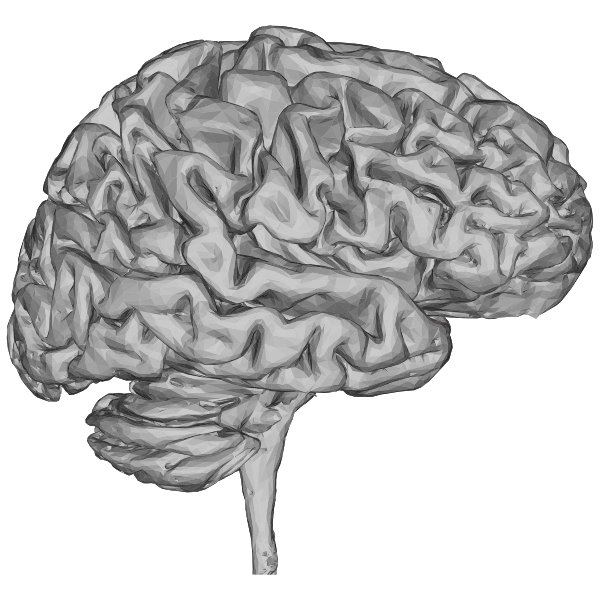
\includegraphics[scale=0.3]{data/brain.png}};
			% \end{axis}
            \newcommand{\mrivsep}{0.52}
                \newcommand{\mrihsep}{0.44}
                \def\plotwidth{11.68}

                \newcommand{\nodesize}{11pt}
                \newcommand{\hsep}{28pt}
                \newcommand{\vsep}{14pt}

                \newcommand{\arrowwidth}{0.05cm}
                \newcommand{\innerarrow}{{Latex[length=0.1cm, width=0.15cm]}}
                \newcommand{\outerarrow}{{Latex[length=0.2cm, width=0.3cm]}}

                \definecolor{cb-green}{HTML}{4dac93}
                \definecolor{cb-blue}{HTML}{3594d6}
                \definecolor{outercolor}{RGB}{128, 128, 128}
                \colorlet{train-fill}{cb-blue}

                \newcommand{\patientlocation}[1]{($ (1, -1.6) + ####1 $)}
                \newcommand{\controllocation}[1]{($ (1, -2.8) + ####1 $)}
                \newcommand{\modellocation}[1]{($ (0.5 * \plotwidth, -2.2) + ####1 $)}

                \node[draw=none, outer sep=0pt, inner sep=1pt] (input) at \modellocation{(-5 * \hsep, 0)} {
                    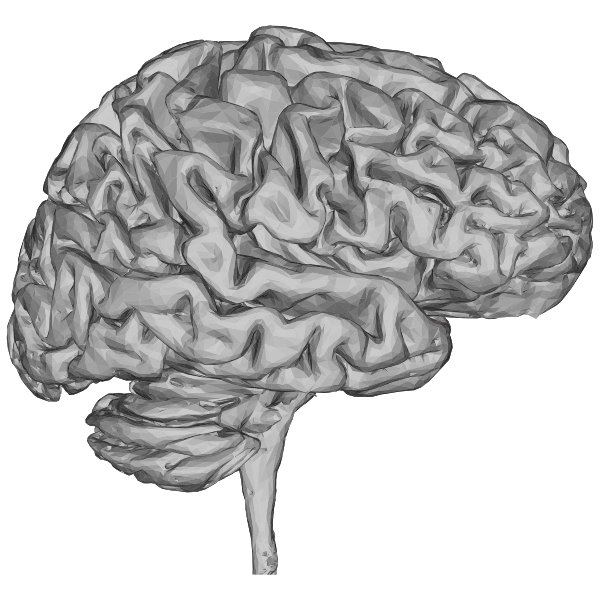
\includegraphics[width=1.5cm] {
                        data/brain.png
                    }
                };

                \newcommand{\padding}{0.2}

                \draw[] (input.north west) -- ($ (input.north east) - (\padding, 0) $)
                        -- ($ (input.south east) - (\padding, -\padding) $)
                        -- ($ (input.south west) - (0, -\padding) $)
                        -- (input.north west);

                        \node[draw=none, outer sep=0pt, inner sep=1pt] (input) at \modellocation{(-5 * \hsep, 0)} {
                            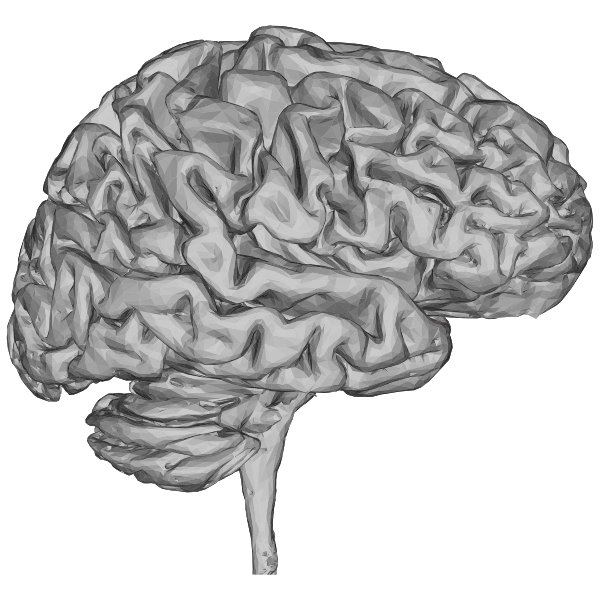
\includegraphics[width=1.5cm] {
                                data/brain.png
                            }
                        };

                \draw[] ($ (input.north west) - (-\padding, \padding) $) -- ($ (input.north east) - (0, \padding) $)
                        -- ($ (input.south east) - (0, 0) $)
                        -- ($ (input.south west) - (-\padding, 0) $)
                        -- ($ (input.north west) - (-\padding, \padding) $);

                \draw[] (input.north west) -- ($ (input.north west) - (-\padding, \padding) $);
                \draw[] ($ (input.south west) - (0, -\padding) $) -- ($ (input.south west) - (-\padding, 0) $);
                \draw[] ($ (input.north east) - (\padding, 0) $) -- ($ (input.north east) - (0, \padding) $);
                \draw[] ($ (input.south east) - (\padding, -\padding) $) -- ($ (input.south east) - (0, 0) $);

                \node[circle, inner sep=0pt, fill=none, outer sep=0pt, line width=0pt, draw=none] (n00) at \modellocation{(-3 * \hsep, 0)} {};

                \node[circle, minimum size=\nodesize, inner sep=0pt, fill=train-fill!35, outer sep=0pt, line width=0pt, draw=train-fill!35] (n10) at \modellocation{(-2 * \hsep, 2 * \vsep)} {};
                \node[circle, minimum size=\nodesize, inner sep=0pt, fill=train-fill, outer sep=0pt, line width=0pt, draw=train-fill] (n11) at \modellocation{(-2 * \hsep, 1 * \vsep)} {};
                \node[circle, minimum size=\nodesize, inner sep=0pt, fill=train-fill!15, outer sep=0pt, line width=0pt, draw=train-fill!15] (n12) at \modellocation{(-2 * \hsep, 0)} {};
                \node[circle, minimum size=\nodesize, inner sep=0pt, fill=train-fill!85, outer sep=0pt, line width=0pt, draw=train-fill!85] (n13) at \modellocation{(-2 * \hsep, -1 * \vsep)} {};
                \node[circle, minimum size=\nodesize, inner sep=0pt, fill=train-fill!90, outer sep=0pt, line width=0pt, draw=train-fill!90] (n14) at \modellocation{(-2 * \hsep, -2 * \vsep)} {};

                \node[circle, minimum size=\nodesize, inner sep=0pt, fill=train-fill!55, outer sep=0pt, line width=0pt, draw=train-fill!55] (n20) at \modellocation{(-1 * \hsep, 1.5 * \vsep)} {};
                \node[circle, minimum size=\nodesize, inner sep=0pt, fill=train-fill!20, outer sep=0pt, line width=0pt, draw=train-fill!20] (n21) at \modellocation{(-1 * \hsep, 0.5 * \vsep)} {};
                \node[circle, minimum size=\nodesize, inner sep=0pt, fill=train-fill!90, outer sep=0pt, line width=0pt, draw=train-fill!50] (n22) at \modellocation{(-1 * \hsep, -0.5 * \vsep)} {};
                \node[circle, minimum size=\nodesize, inner sep=0pt, fill=train-fill!35, outer sep=0pt, line width=0pt, draw=train-fill!35] (n23) at \modellocation{(-1 * \hsep, -1.5 * \vsep)} {};

                \node[circle, minimum size=\nodesize, inner sep=0pt, fill=train-fill!95, outer sep=0pt, line width=0pt, draw=train-fill!65] (n30) at \modellocation{(0 * \hsep, 1.5 * \vsep)} {};
                \node[circle, minimum size=\nodesize, inner sep=0pt, fill=train-fill!20, outer sep=0pt, line width=0pt, draw=train-fill!20] (n31) at \modellocation{(0 * \hsep, 0.5 * \vsep)} {};
                \node[circle, minimum size=\nodesize, inner sep=0pt, fill=train-fill!90, outer sep=0pt, line width=0pt, draw=train-fill!90] (n32) at \modellocation{(0 * \hsep, -0.5 * \vsep)} {};
                \node[circle, minimum size=\nodesize, inner sep=0pt, fill=train-fill!80, outer sep=0pt, line width=0pt, draw=train-fill!80] (n33) at \modellocation{(0 * \hsep, -1.5 * \vsep)} {};

                \node[circle, minimum size=\nodesize, inner sep=0pt, fill=train-fill!50, outer sep=0pt, line width=0pt, draw=train-fill!50] (n40) at \modellocation{(1 * \hsep, 1*\vsep)} {};
                \node[circle, minimum size=\nodesize, inner sep=0pt, fill=train-fill!90, outer sep=0pt, line width=0pt, draw=train-fill!70] (n41) at \modellocation{(1 * \hsep, 0*\vsep)} {};
                \node[circle, minimum size=\nodesize, inner sep=0pt, fill=train-fill!70, outer sep=0pt, line width=0pt, draw=train-fill!30] (n42) at \modellocation{(1 * \hsep, -1*\vsep)} {};

                \node[circle, minimum size=\nodesize, inner sep=0pt, fill=train-fill, outer sep=0pt, line width=0pt, draw=train-fill] (n50) at \modellocation{(2 * \hsep, 1*\vsep)} {};
                \node[circle, minimum size=\nodesize, inner sep=0pt, fill=train-fill!70, outer sep=0pt, line width=0pt, draw=train-fill!70] (n51) at \modellocation{(2 * \hsep, 0*\vsep)} {};
                \node[circle, minimum size=\nodesize, inner sep=0pt, fill=train-fill!30, outer sep=0pt, line width=0pt, draw=train-fill!30] (n52) at \modellocation{(2 * \hsep, -1*\vsep)} {};

                \node[circle, minimum size=\nodesize, inner sep=0pt, fill=train-fill!80, outer sep=0pt, line width=0pt, draw=train-fill!65] (n60) at \modellocation{(3 * \hsep, 0)} {};

                \node[align=center, font=\scriptsize\linespread{0.8}\selectfont] (loss) at (0.5+2*4.85, -2.2) {Predicted\\brain age};

                \draw[
                    color=train-fill!35,
                    -\innerarrow,
                    line width=\arrowwidth
                ] (n00) to [out=20,in=200] (n10) {};
                \draw[
                    color=train-fill,
                    -\innerarrow,
                    line width=\arrowwidth
                ] (n00) to [out=10,in=190] (n11) {};
                \draw[
                    color=train-fill!15,
                    -\innerarrow,
                    line width=\arrowwidth
                ] (n00) to [out=0,in=180] (n12) {};
                \draw[
                    color=train-fill!85,
                    -\innerarrow,
                    line width=\arrowwidth
                ] (n00) to [out=-10,in=170] (n13) {};
                \draw[
                    color=train-fill!90,
                    -\innerarrow,
                    line width=\arrowwidth
                ] (n00) to [out=-20,in=160] (n14) {};

                \draw[
                    color=train-fill!35,
                    -\innerarrow,
                    line width=\arrowwidth
                ] (n10) to [out=-5,in=175] (n20) {};
                \draw[
                    color=train-fill!10,
                    -\innerarrow,
                    line width=\arrowwidth
                ] (n10) to [out=-15,in=165] (n21) {};
                \draw[
                    color=train-fill!70,
                    -\innerarrow,
                    line width=\arrowwidth
                ] (n10) to [out=-25,in=155] (n22) {};
                \draw[
                    color=train-fill!50,
                    -\innerarrow,
                    line width=\arrowwidth
                ] (n10) to [out=-35,in=145] (n23) {};

                \draw[
                    color=train-fill!30,
                    -\innerarrow,
                    line width=\arrowwidth
                ] (n11) to [out=5,in=185] (n20) {};
                \draw[
                    color=train-fill!25,
                    -\innerarrow,
                    line width=\arrowwidth
                ] (n11) to [out=-5,in=175] (n21) {};
                \draw[
                    color=train-fill!95,
                    -\innerarrow,
                    line width=\arrowwidth
                ] (n11) to [out=-15,in=165] (n22) {};
                \draw[
                    color=train-fill!35,
                    -\innerarrow,
                    line width=\arrowwidth
                ] (n11) to [out=-25,in=155] (n23) {};

                \draw[
                    color=train-fill!70,
                    -\innerarrow,
                    line width=\arrowwidth
                ] (n12) to [out=15,in=195] (n20) {};
                \draw[
                    color=train-fill!20,
                    -\innerarrow,
                    line width=\arrowwidth
                ] (n12) to [out=5,in=185] (n21) {};
                \draw[
                    color=train-fill!80,
                    -\innerarrow,
                    line width=\arrowwidth
                ] (n12) to [out=-5,in=175] (n22) {};
                \draw[
                    color=train-fill,
                    -\innerarrow,
                    line width=\arrowwidth
                ] (n12) to [out=-15,in=165] (n23) {};

                \draw[
                    color=train-fill!40,
                    -\innerarrow,
                    line width=\arrowwidth
                ] (n13) to [out=25,in=205] (n20) {};
                \draw[
                    color=train-fill!35,
                    -\innerarrow,
                    line width=\arrowwidth
                ] (n13) to [out=15,in=195] (n21) {};
                \draw[
                    color=train-fill!20,
                    -\innerarrow,
                    line width=\arrowwidth
                ] (n13) to [out=5,in=185] (n22) {};
                \draw[
                    color=white,
                    -\innerarrow,
                    line width=\arrowwidth
                ] (n13) to [out=-5,in=175] (n23) {};

                \draw[
                    color=train-fill!40,
                    -\innerarrow,
                    line width=\arrowwidth
                ] (n14) to [out=35,in=215] (n20) {};
                \draw[
                    color=train-fill!85,
                    -\innerarrow,
                    line width=\arrowwidth
                ] (n14) to [out=25,in=205] (n21) {};
                \draw[
                    color=train-fill!35,
                    -\innerarrow,
                    line width=\arrowwidth
                ] (n14) to [out=15,in=195] (n22) {};
                \draw[
                    color=train-fill,
                    -\innerarrow,
                    line width=\arrowwidth
                ] (n14) to [out=5,in=185] (n23) {};

                \draw[
                    color=train-fill!85,
                    -\innerarrow,
                    line width=\arrowwidth
                ] (n20) to [out=0,in=180] (n30) {};
                \draw[
                    color=train-fill!50,
                    -\innerarrow,
                    line width=\arrowwidth
                ] (n20) to [out=-10,in=170] (n31) {};
                \draw[
                    color=train-fill!75,
                    -\innerarrow,
                    line width=\arrowwidth
                ] (n20) to [out=-20,in=160] (n32) {};
                \draw[
                    color=white,
                    -\innerarrow,
                    line width=\arrowwidth
                ] (n20) to [out=-30,in=150] (n33) {};

                \draw[
                    color=train-fill,
                    -\innerarrow,
                    line width=\arrowwidth
                ] (n21) to [out=10,in=190] (n30) {};
                \draw[
                    color=train-fill!30,
                    -\innerarrow,
                    line width=\arrowwidth
                ] (n21) to [out=0,in=180] (n31) {};
                \draw[
                    color=train-fill!25,
                    -\innerarrow,
                    line width=\arrowwidth
                ] (n21) to [out=-10,in=170] (n32) {};
                \draw[
                    color=white,
                    -\innerarrow,
                    line width=\arrowwidth
                ] (n21) to [out=-20,in=160] (n33) {};

                \draw[
                    color=train-fill!35,
                    -\innerarrow,
                    line width=\arrowwidth
                ] (n22) to [out=20,in=200] (n30) {};
                \draw[
                    color=train-fill!95,
                    -\innerarrow,
                    line width=\arrowwidth
                ] (n22) to [out=10,in=190] (n31) {};
                \draw[
                    color=train-fill!80,
                    -\innerarrow,
                    line width=\arrowwidth
                ] (n22) to [out=0,in=180] (n32) {};
                \draw[
                    color=white,
                    -\innerarrow,
                    line width=\arrowwidth
                ] (n22) to [out=-10,in=170] (n33) {};

                \draw[
                    color=train-fill!45,
                    -\innerarrow,
                    line width=\arrowwidth
                ] (n23) to [out=30,in=210] (n30) {};
                \draw[
                    color=train-fill!70,
                    -\innerarrow,
                    line width=\arrowwidth
                ] (n23) to [out=20,in=200] (n31) {};
                \draw[
                    color=train-fill!10,
                    -\innerarrow,
                    line width=\arrowwidth
                ] (n23) to [out=10,in=190] (n32) {};
                \draw[
                    color=train-fill!20,
                    -\innerarrow,
                    line width=\arrowwidth
                ] (n23) to [out=0,in=180] (n33) {};

                \draw[
                    color=train-fill!50,
                    -\innerarrow,
                    line width=\arrowwidth
                ] (n30) to [out=-5,in=175] (n40) {};
                \draw[
                    color=train-fill!30,
                    -\innerarrow,
                    line width=\arrowwidth
                ] (n30) to [out=-15,in=165] (n41) {};
                \draw[
                    color=train-fill,
                    -\innerarrow,
                    line width=\arrowwidth
                ] (n30) to [out=-25,in=155] (n42) {};

                \draw[
                    color=train-fill!45,
                    -\innerarrow,
                    line width=\arrowwidth
                ] (n31) to [out=5,in=185] (n40) {};
                \draw[
                    color=train-fill!90,
                    -\innerarrow,
                    line width=\arrowwidth
                ] (n31) to [out=-5,in=175] (n41) {};
                \draw[
                    color=train-fill!45,
                    -\innerarrow,
                    line width=\arrowwidth
                ] (n31) to [out=-15,in=165] (n42) {};

                \draw[
                    color=train-fill!15,
                    -\innerarrow,
                    line width=\arrowwidth
                ] (n32) to [out=15,in=195] (n40) {};
                \draw[
                    color=train-fill!70,
                    -\innerarrow,
                    line width=\arrowwidth
                ] (n32) to [out=5,in=185] (n41) {};
                \draw[
                    color=train-fill!50,
                    -\innerarrow,
                    line width=\arrowwidth
                ] (n32) to [out=-5,in=175] (n42) {};

                \draw[
                    color=train-fill!40,
                    -\innerarrow,
                    line width=\arrowwidth
                ] (n33) to [out=25,in=205] (n40) {};
                \draw[
                    color=train-fill!20,
                    -\innerarrow,
                    line width=\arrowwidth
                ] (n33) to [out=15,in=195] (n41) {};
                \draw[
                    color=train-fill!90,
                    -\innerarrow,
                    line width=\arrowwidth
                ] (n33) to [out=5,in=185] (n42) {};

                \draw[
                    color=train-fill!25,
                    -\innerarrow,
                    line width=\arrowwidth
                ] (n40) to [out=0,in=180] (n50) {};
                \draw[
                    color=train-fill!15,
                    -\innerarrow,
                    line width=\arrowwidth
                ] (n40) to [out=-10,in=170] (n51) {};
                \draw[
                    color=train-fill,
                    -\innerarrow,
                    line width=\arrowwidth
                ] (n40) to [out=-20,in=160] (n52) {};

                \draw[
                    color=train-fill!35,
                    -\innerarrow,
                    line width=\arrowwidth
                ] (n41) to [out=10,in=190] (n50) {};
                \draw[
                    color=train-fill!10,
                    -\innerarrow,
                    line width=\arrowwidth
                ] (n41) to [out=0,in=180] (n51) {};
                \draw[
                    color=train-fill!90,
                    -\innerarrow,
                    line width=\arrowwidth
                ] (n41) to [out=-10,in=170] (n52) {};

                \draw[
                    color=train-fill!50,
                    -\innerarrow,
                    line width=\arrowwidth
                ] (n42) to [out=20,in=200] (n50) {};
                \draw[
                    color=train-fill!40,
                    -\innerarrow,
                    line width=\arrowwidth
                ] (n42) to [out=10,in=190] (n51) {};
                \draw[
                    color=train-fill!20,
                    -\innerarrow,
                    line width=\arrowwidth
                ] (n42) to [out=0,in=180] (n52) {};

                \draw[
                    color=train-fill!80,
                    -\innerarrow,
                    line width=\arrowwidth,
                ] (n50) to [out=-10,in=170] (n60) {};
                \draw[
                    color=train-fill!90,
                    -\innerarrow,
                    line width=\arrowwidth,
                ] (n51) to [out=0,in=180] (n60) {};
                \draw[
                    color=train-fill!30,
                    -\innerarrow,
                    line width=\arrowwidth,
                ] (n52) to [out=10,in=190] (n60) {};

                \draw[black] (n00.center) --
                             ($ (n00) + (0, 2*\vsep+0.5*\nodesize+2pt) $) --
                             ($ (n00) + (6*\hsep+0.5*\nodesize+2pt, 2*\vsep+0.5*\nodesize+2pt) $) --
                             ($ (n00) + (6*\hsep+0.5*\nodesize+2pt, -2*\vsep-0.5*\nodesize-2pt) $) --
                             ($ (n00) + (0, -2*\vsep-0.5*\nodesize-2pt) $) --
                             (n00.center);

                \node[] at ($ (n30) + (0, \vsep+0.5*\nodesize) $) {\scriptsize{Convolutional Neural Network}};

                \draw[
                    color=outercolor,
                    -\outerarrow,
                    line width=0.1cm
                ] ($ (n00.west) - (1, 0) $) to [out=0,in=180] (n00) {};
                \draw[
                    color=outercolor,
                    -\outerarrow,
                    line width=0.1cm
                ] (n60) to [out=0,in=180] (loss) {};
		\end{tikzpicture}
        \vfill
        CNN with $\sim$3m parameters predicting brain age from raw imaging data
	\end{frame}

	\begin{frame}{Brain age: Predictions}
		\def\N{1}
		\centering
		\vfill
		\begin{tikzpicture}
			\begin{groupplot}[
				group style={
					group size=2 by 1,
					horizontal sep=1.2cm,
					vertical sep=0.8cm
				},
				width=0.5\linewidth,
				height=0.5\linewidth
			]

			   \nextgroupplot[
				  xmin=0,
				  xmax=100,
				  ymin=0,
				  ymax=100,
				  xtick pos=bottom,
				  ytick pos=left,
				  ticklabel style = {font=\footnotesize},
				  xlabel=\footnotesize{Chronological age},
				  ylabel=\footnotesize{Predicted brain age},
				  title={Test set}
			  ]
				  \addplot [red] coordinates {(0,0) (100,100)};
				  \addplot [
					  only marks,
					  mark size=1.5pt,
					  color=black,
					  opacity=0.35
				  ] table [
					  x=regression,
					  y=age,
					  each nth point={\N},
					  col sep=comma
				  ] {data/paper1/prediction/test_predictions.csv};
				  \node [anchor=south east,inner sep=0pt,outer sep=0pt] (outofsample) at (rel axis cs:0.92,0.08) {\footnotesize{\textcolor{red}{MAE=2.47}}};

			  \nextgroupplot[
				  xmin=0,
				  xmax=100,
				  ymin=0,
				  ymax=100,
				  xtick pos=bottom,
				  ytick pos=left,
				  ticklabel style = {font=\footnotesize},
				  title={External test set}
			  ]
				  \addplot [red] coordinates {(0,0) (100,100)};
				  \addplot [
					  only marks,
					  mark size=1.5pt,
					  color=black,
					  opacity=0.35
				  ] table [
					  x=regression,
					  y=age,
					  each nth point={\N},
					  col sep=comma
				  ] {data/paper1/prediction/external_predictions.csv};
				  \node [anchor=south east,inner sep=0pt,outer sep=0pt] (outofsample) at (rel axis cs:0.92,0.08) {\footnotesize{\textcolor{red}{MAE=3.90}}};
		\end{groupplot}
	  \end{tikzpicture}
	  \vfill
      Mean absolute error of 3.9 years in data from unseen scanners
	\end{frame}

	\begin{frame}{Brain age: Associations}
        \centering
        \vfill

  \begin{columns}[T] % T aligns the top of the columns
    \column{0.6\textwidth} % Adjust the width of the first column
		\begin{tikzpicture}
            \begin{axis}[
                    width=1.15\textwidth,
                    height=\textwidth,
                    ylabel=$-\mathrm{log}_{10}(p)$,
                    y label style={at={(-0.06, 0.5)}},
                    ymin=0,
                    ymax=11.5,
                    xmin=-1,
                    xmax=395,
                    ytick={2,4,6,8,10},
                    yticklabels={-2,-4,-6,-8,-10},
                    axis x line*=bottom,
                    axis y line=left,
                    xtick={32.5,102.5,149.5,177.5,208.5,
                           233,254.5,275.5,301.5,334.5,
                           358,372,388},
                    xticklabels={1,2,3,4,5,6,7,8,9,10,
                                 11,12,13},
                    tick label style={font=\scriptsize},
                    clip=false
                ]
                \addplot[draw=black, only marks, mark size=1.5pt, fill=pwas] table [x=x,y=y] {\pwas};
                \addplot[draw=black,dashed] coordinates {(-1, 3.896) (395, 3.896)};
                \addplot[draw=black,dotted] coordinates {(65,0) (65,11.5)};
                \addplot[draw=black,dotted] coordinates {(140,0) (140,11.5)};
                \addplot[draw=black,dotted] coordinates {(159,0) (159,11.5)};
                \addplot[draw=black,dotted] coordinates {(196,0) (196,11.5)};
                \addplot[draw=black,dotted] coordinates {(221,0) (221,11.5)};
                \addplot[draw=black,dotted] coordinates {(245,0) (245,11.5)};
                \addplot[draw=black,dotted] coordinates {(264,0) (264,11.5)};
                \addplot[draw=black,dotted] coordinates {(287,0) (287,11.5)};
                \addplot[draw=black,dotted] coordinates {(316,0) (316,11.5)};
                \addplot[draw=black,dotted] coordinates {(353,0) (353,11.5)};
                \addplot[draw=black,dotted] coordinates {(363,0) (363,11.5)};
                \addplot[draw=black,dotted] coordinates {(381,0) (381,11.5)};
                \addplot[draw=black,dotted] coordinates {(395,0) (395,11.5)};
                \node[anchor=south] at (axis cs:12,6.09) {\tiny{HbA1c}};
                \node[anchor=south] at (axis cs:18,10.49) {\tiny{Glucose}};
                \node[anchor=north] at (axis cs:26,10.23) {\tiny{IGF-1}};
                \node[anchor=south] at (axis cs:49,4.47) {\tiny{Corpuscular volume}};
                \node[anchor=south, align=center] at (axis cs:65,6.72) {\tiny{Vascular/heart}\\[-1.5ex] \tiny{problem}};
                \node[anchor=south, align=center] at (axis cs:89,9.93) {\tiny{Blood pressure}\\[-1.5ex] \tiny{medication}};
                %\node[anchor=north] at (axis cs:107,6.33) {\tiny{Diabetes related eye disease}};
                \node[anchor=south] at (axis cs:128,6.64) {\tiny{Diabetes}};
                %\node[anchor=south] at (axis cs:141,4.22) {\tiny{Other group activity}};
                %\node[anchor=east] at (axis cs:204,5.48) {\tiny{SBP}};
                %\node[anchor=west] at (axis cs:208,5.59) {\tiny{DBP}};
                %\node[anchor=south] at (axis cs:232,6.11) {\tiny{Cereal intake}};
                %\node[anchor=south] at (axis cs:245,3.95) {\tiny{Alcohol intake frequency}};
                \node[anchor=south] at (axis cs:254,6.94) {\tiny{Weekly beer/cider intake}};
                %\node[anchor=north, align=center] at (axis cs:287,4.11) {\tiny{Age}\\[-1.5ex] \tiny{stopped}\\[-1.5ex] \tiny{smoking}};
                \node[anchor=south, align=center] at (axis cs:303,4.61) {\tiny{Total cigarette}\\[-1.5ex] \tiny{packs}};
                %\node[anchor=north] at (axis cs:330,4.06) {\tiny{Pack years}};
                %\node[anchor=south] at (axis cs:354,4.08) {\tiny{Number in household}};
                \node[anchor=south, align=center] at (axis cs:376,5.33) {\tiny{Non-UK country}\\[-1.5ex] \tiny{of birth}};
            \end{axis}
        \end{tikzpicture}

    \column{0.4\textwidth} % Adjust the width of the second column
        \vspace*{-0.17cm}
        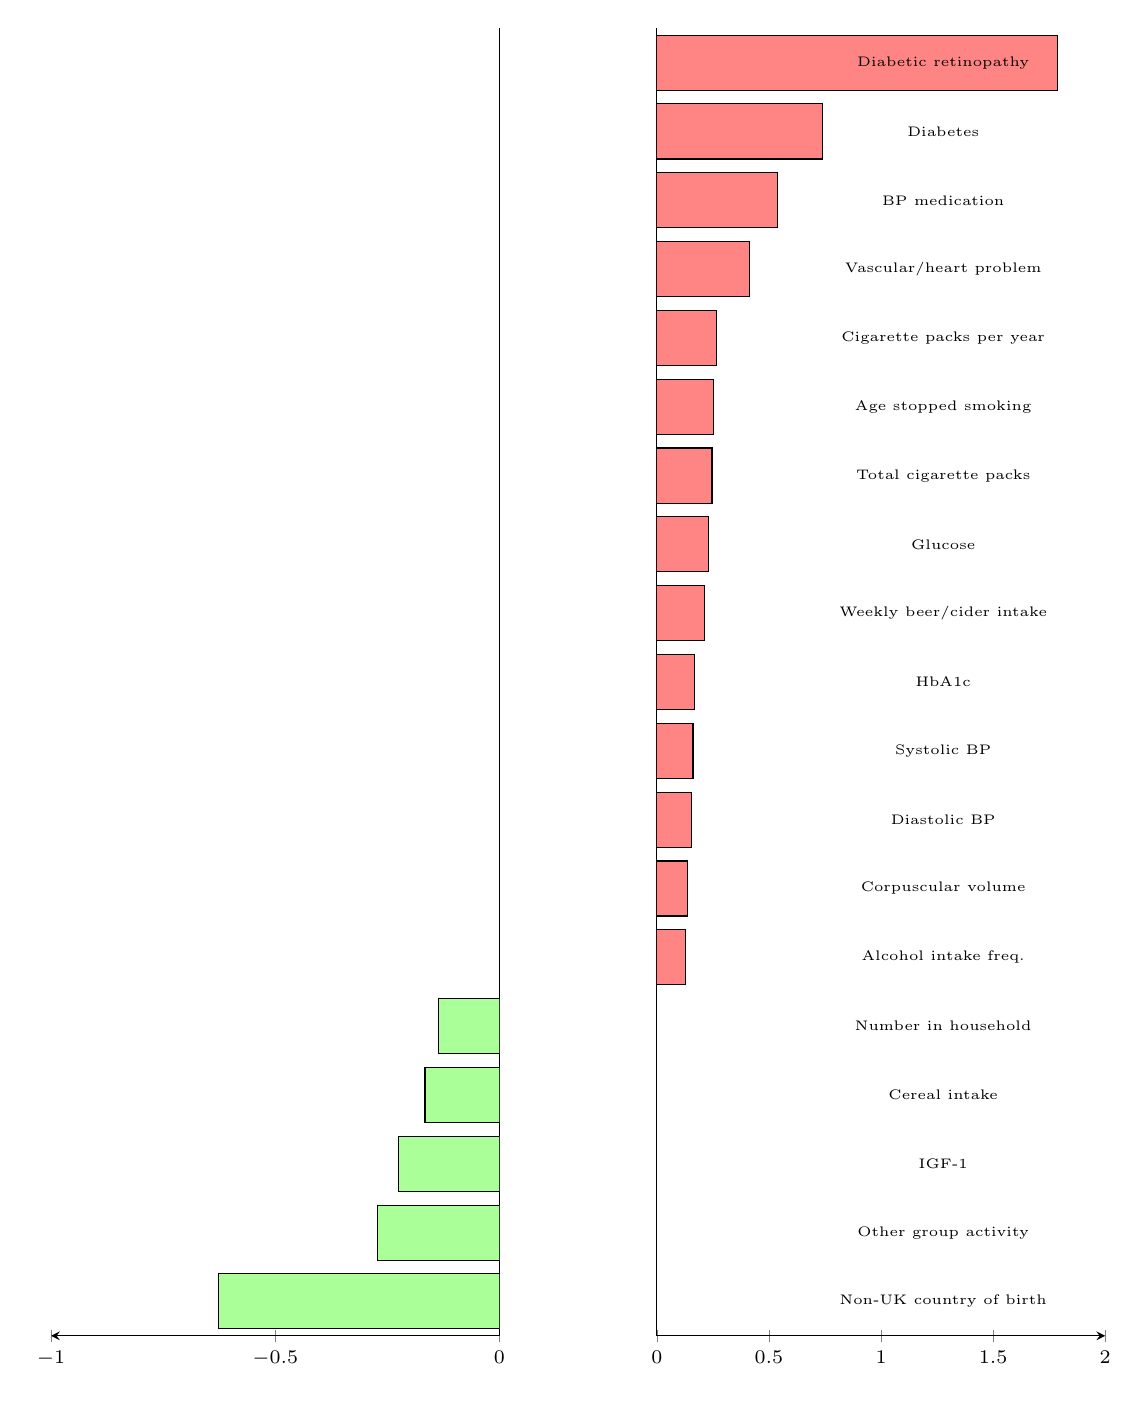
\begin{tikzpicture}
            \begin{groupplot}[
                group style={
                              group size=2 by 1,
                              horizontal sep=2cm
                          },
                          width=0.6\textwidth,
                          height=1.5\textwidth,
                  ]
                \nextgroupplot[
                    yticklabels={,,},
                    xmin=-1,
                    xmax=0,
                    xtick={0, -0.5, -1},
                    ymin=0,
                    ymax=19,
                    axis x line=bottom,
                    axis y line*=right,
                    x axis line style={stealth-},
                    ymajorticks=false,
                    tick label style={font=\scriptsize}
                ]
                    \addplot[fill=neg] coordinates {
                        (0,0.1)
                        (0,0.9)
                        (-0.627,0.9)
                        (-0.627,0.1)
                        (0,0.1)
                    };

                    \addplot[fill=neg] coordinates {
                        (0,1.1)
                        (0,1.9)
                        (-0.272,1.9)
                        (-0.272,1.1)
                        (0,1.1)
                    };

                    \addplot[fill=neg] coordinates {
                        (0,2.1)
                        (0,2.9)
                        (-0.225,2.9)
                        (-0.225,2.1)
                        (0,2.1)
                    };

                    \addplot[fill=neg] coordinates {
                        (0,3.1)
                        (0,3.9)
                        (-0.166,3.9)
                        (-0.166,3.1)
                        (0,3.1)
                    };

                    \addplot[fill=neg] coordinates {
                        (0,4.1)
                        (0,4.9)
                        (-0.136,4.9)
                        (-0.136,4.1)
                        (0,4.1)
                    };

                    \coordinate (1) at (axis cs: 0.99,0.5) {};
                    \coordinate (2) at (axis cs: 0.99,1.5) {};
                    \coordinate (3) at (axis cs: 0.99,2.5) {};
                    \coordinate (4) at (axis cs: 0.99,3.5) {};
                    \coordinate (5) at (axis cs: 0.99,4.5) {};
                    \coordinate (6) at (axis cs: 0.99,5.5) {};
                    \coordinate (7) at (axis cs: 0.99,6.5) {};
                    \coordinate (8) at (axis cs: 0.99,7.5) {};
                    \coordinate (9) at (axis cs: 0.99,8.5) {};
                    \coordinate (10) at (axis cs: 0.99,9.5) {};
                    \coordinate (11) at (axis cs: 0.99,10.5) {};
                    \coordinate (12) at (axis cs: 0.99,11.5) {};
                    \coordinate (13) at (axis cs: 0.99,12.5) {};
                    \coordinate (14) at (axis cs: 0.99,13.5) {};
                    \coordinate (15) at (axis cs: 0.99,14.5) {};
                    \coordinate (16) at (axis cs: 0.99,15.5) {};
                    \coordinate (17) at (axis cs: 0.99,16.5) {};
                    \coordinate (18) at (axis cs: 0.99,17.5) {};
                    \coordinate (19) at (axis cs: 0.99,18.5) {};
                \nextgroupplot[
                    yticklabels={,,},
                    xmin=0,
                    xmax=2,
                    ymin=0,
                    ymax=19,
                    axis x line=bottom,
                    axis y line*=left,
                    ymajorticks=false,,
                    tick label style={font=\scriptsize}
                ]

                    \addplot[fill=pos] coordinates {
                            (0,5.1)
                            (0,5.9)
                            (0.127,5.9)
                            (0.127,5.1)
                            (0,5.1)
                        };

                        \addplot[fill=pos] coordinates {
                            (0,6.1)
                            (0,6.9)
                            (0.137,6.9)
                            (0.137,6.1)
                            (0,6.1)
                        };

                        \addplot[fill=pos] coordinates {
                            (0,7.1)
                            (0,7.9)
                            (0.156,7.9)
                            (0.156,7.1)
                            (0,7.1)
                        };

                        \addplot[fill=pos] coordinates {
                            (0,8.1)
                            (0,8.9)
                            (0.161,8.9)
                            (0.161,8.1)
                            (0,8.1)
                        };

                        \addplot[fill=pos] coordinates {
                            (0,9.1)
                            (0,9.9)
                            (0.169,9.9)
                            (0.169,9.1)
                            (0,9.1)
                        };

                        \addplot[fill=pos] coordinates {
                            (0,10.1)
                            (0,10.9)
                            (0.211,10.9)
                            (0.211,10.1)
                            (0,10.1)
                        };

                        \addplot[fill=pos] coordinates {
                            (0,11.1)
                            (0,11.9)
                            (0.230,11.9)
                            (0.230,11.1)
                            (0,11.1)
                        };

                        \addplot[fill=pos] coordinates {
                            (0,12.1)
                            (0,12.9)
                            (0.246,12.9)
                            (0.246,12.1)
                            (0,12.1)
                        };

                        \addplot[fill=pos] coordinates {
                            (0,13.1)
                            (0,13.9)
                            (0.251,13.9)
                            (0.251,13.1)
                            (0,13.1)
                        };

                        \addplot[fill=pos] coordinates {
                            (0,14.1)
                            (0,14.9)
                            (0.265,14.9)
                            (0.265,14.1)
                            (0,14.1)
                        };

                        \addplot[fill=pos] coordinates {
                            (0,15.1)
                            (0,15.9)
                            (0.415,15.9)
                            (0.415,15.1)
                            (0,15.1)
                        };

                        \addplot[fill=pos] coordinates {
                            (0,16.1)
                            (0,16.9)
                            (0.540,16.9)
                            (0.540,16.1)
                            (0,16.1)
                        };

                        \addplot[fill=pos] coordinates {
                            (0,17.1)
                            (0,17.9)
                            (0.74,17.9)
                            (0.74,17.1)
                            (0,17.1)
                        };

                        \addplot[fill=pos] coordinates {
                            (0,18.1)
                            (0,18.9)
                            (1.786,18.9)
                            (1.786,18.1)
                            (0,18.1)
                        };

        \end{groupplot}
        \node [align=center,font=\tiny\linespread{0.8}\selectfont] at (1) {Non-UK country of birth};
        \node [align=center,font=\tiny\linespread{0.8}\selectfont] at (2) {Other group activity};
        \node [align=center,font=\tiny\linespread{0.8}\selectfont] at (3) {IGF-1};
        \node [align=center,font=\tiny\linespread{0.8}\selectfont] at (4) {Cereal intake};
        \node [align=center,font=\tiny\linespread{0.8}\selectfont] at (5) {Number in household};
        \node [align=center,font=\tiny\linespread{0.8}\selectfont] at (6) {Alcohol intake freq.};
        \node [align=center,font=\tiny\linespread{0.8}\selectfont] at (7) {Corpuscular volume};
        \node [align=center,font=\tiny\linespread{0.8}\selectfont] at (8) {Diastolic BP};
        \node [align=center,font=\tiny\linespread{0.8}\selectfont] at (9) {Systolic BP};
        \node [align=center,font=\tiny\linespread{0.8}\selectfont] at (10) {HbA1c};
        \node [align=center,font=\tiny\linespread{0.8}\selectfont] at (11) {Weekly beer/cider intake};
        \node [align=center,font=\tiny\linespread{0.8}\selectfont] at (12) {Glucose};
        \node [align=center,font=\tiny\linespread{0.8}\selectfont] at (13) {Total cigarette packs};
        \node [align=center,font=\tiny\linespread{0.8}\selectfont] at (14) {Age stopped smoking};
        \node [align=center,font=\tiny\linespread{0.8}\selectfont] at (15) {Cigarette packs per year};
        \node [align=center,font=\tiny\linespread{0.8}\selectfont] at (16) {Vascular/heart problem};
        \node [align=center,font=\tiny\linespread{0.8}\selectfont] at (17) {BP medication};
        \node [align=center,font=\tiny\linespread{0.8}\selectfont] at (18) {Diabetes};
        \node [align=center,font=\tiny\linespread{0.8}\selectfont] at (19) {Diabetic retinopathy};
        \end{tikzpicture}
    \end{columns}
    \vfill
    Higher brain age associated with diabetes, vascular disease, smoking, alcohol
	\end{frame}

	\begin{frame}{Brain age: Patient cohorts}
        \centering
        \vfill
		\begin{figure}
			\begin{center}
				\begin{tikzpicture}
					\begin{axis}[
						height=0.7\textwidth,
						width=\textwidth,
						axis x line=bottom,
						hide y axis,
						xmin=-19,
						xmax=19,
						ymin=-0.1,
						ymax=6.6,
						xlabel=Brain age delta,
						axis line style={latex-latex}
					]
						\addplot [black, dashed] coordinates {(0,-0.3) (0,9)};

						\addplot [blue,very thick,name path=MScontrols] table [x=x,y expr=\thisrow{control} + 5.5] {\MSdelta};
						\addplot [red,very thick,name path=MSpatients] table [x=x,y expr=\thisrow{patient} + 5.5] {\MSdelta};
						\addplot [draw=none,name path=MSbaseline] coordinates {(-20,5.5) (20,5.5)};
						\addplot [blue,fill opacity=0.3] fill between [of=MScontrols and MSbaseline];
						\addplot [red,fill opacity=0.3] fill between [of=MSpatients and MSbaseline];
						\coordinate (MS) at (axis cs:11.8,6.7) {};
						\addplot [blue,very thick,name path=ADcontrols] table [x=x,y expr=\thisrow{control} + 4.4] {\ADdelta};
						\addplot [red,very thick,name path=ADpatients] table [x=x,y expr=\thisrow{patient} + 4.4] {\ADdelta};
						\addplot [draw=none,name path=ADbaseline] coordinates {(-20,4.4) (20,4.4)};
						\addplot [blue,fill opacity=0.3] fill between [of=ADcontrols and ADbaseline];
						\addplot [red,fill opacity=0.3] fill between [of=ADpatients and ADbaseline];
						\coordinate (AD) at (axis cs:11.8,5.6) {};
						\addplot [blue,very thick,name path=MCIcontrols] table [x=x,y expr=\thisrow{control} + 3.3] {\MCIdelta};
						\addplot [red,very thick,name path=MCIpatients] table [x=x,y expr=\thisrow{patient} + 3.3] {\MCIdelta};
						\addplot [draw=none,name path=MCIbaseline] coordinates {(-20,3.3) (20,3.3)};
						\addplot [blue,fill opacity=0.3] fill between [of=MCIcontrols and MCIbaseline];
						\addplot [red,fill opacity=0.3] fill between [of=MCIpatients and MCIbaseline];
						\coordinate (MCI) at (axis cs:11.8,4.5) {};
						\addplot [blue,very thick,name path=SCZcontrols] table [x=x,y expr=\thisrow{control} + 2.2] {\SCZdelta};
						\addplot [red,very thick,name path=SCZpatients] table [x=x,y expr=\thisrow{patient} + 2.2] {\SCZdelta};
						\addplot [draw=none,name path=SCZbaseline] coordinates {(-20,2.2) (20,2.2)};
						\addplot [blue,fill opacity=0.3] fill between [of=SCZcontrols and SCZbaseline];
						\addplot [red,fill opacity=0.3] fill between [of=SCZpatients and SCZbaseline];
						\coordinate (SCZ) at (axis cs:11.8,3.4) {};
						\addplot [blue,very thick,name path=PSYcontrols] table [x=x,y expr=\thisrow{control} + 1.1] {\PSYdelta};
						\addplot [red,very thick,name path=PSYpatients] table [x=x,y expr=\thisrow{patient} + 1.1] {\PSYdelta};
						\addplot [draw=none,name path=PSYbaseline] coordinates {(-20,1.1) (20,1.1)};
						\addplot [blue,fill opacity=0.3] fill between [of=PSYcontrols and PSYbaseline];
						\addplot [red,fill opacity=0.3] fill between [of=PSYpatients and PSYbaseline];
						\coordinate (PSY) at (axis cs:11.8,2.3) {};
						\addplot [blue,very thick,name path=MOODcontrols] table [x=x,y expr=\thisrow{control}] {\MOODdelta};
						\addplot [red,very thick,name path=MOODpatients] table [x=x,y expr=\thisrow{patient}] {\MOODdelta};
						\addplot [draw=none,name path=MOODbaseline] coordinates {(-20,0) (20,0)};
						\addplot [blue,fill opacity=0.3] fill between [of=MOODcontrols and MOODbaseline];
						\addplot [red,fill opacity=0.3] fill between [of=MOODpatients and MOODbaseline];
						\coordinate (MOOD) at (axis cs:11.8,1.2) {};
					\end{axis}
					\matrix [
						matrix of nodes,
						draw=none,
						row sep=-0.18cm,
						anchor=north west,
						column 1/.style={anchor=base west, nodes={font=\tiny}}
					] at (MS) {
						\textbf{MS} \\
						$\Delta=4.42$\\
						$p=1.71*10^{-22}$\\
						$d=0.87$\\
					};
					\matrix [
						matrix of nodes,
						draw=none,
						row sep=-0.18cm,
						anchor=north west,
						column 1/.style={anchor=base west, nodes={font=\tiny}}
					] at (AD) {
						\textbf{AD} \\
						$\Delta=2.81$\\
						$p=4.27*10^{-20}$\\
						$d=0.58$\\
					};
					\matrix [
						matrix of nodes,
						draw=none,
						row sep=-0.18cm,
						anchor=north west,
						column 1/.style={anchor=base west, nodes={font=\tiny}}
					] at (MCI) {
						\textbf{MCI} \\
						$\Delta=2.13$\\
						$p=1.25*10^{-15}$\\
						$d=0.46$\\
					};
					\matrix [
						matrix of nodes,
						draw=none,
						row sep=-0.18cm,
						anchor=north west,
						column 1/.style={anchor=base west, nodes={font=\tiny}}
					] at (SCZ) {
						\textbf{SCZ} \\
						$\Delta=1.40$\\
						$p=4.29*10^{-5}$\\
						$d=0.34$\\
					};
					\matrix [
						matrix of nodes,
						draw=none,
						row sep=-0.18cm,
						anchor=north west,
						column 1/.style={anchor=base west, nodes={font=\tiny}}
					] at (PSY) {
						\textbf{PSY} \\
						$\Delta=0.74$\\
						$p=0.15$\textcolor{white}{$5^2$}\\
						$d=0.20$\\
					};
					\matrix [
						matrix of nodes,
						draw=none,
						row sep=-0.18cm,
						anchor=north west,
						column 1/.style={anchor=base west, nodes={font=\tiny}}
					] at (MOOD) {
						\textbf{MOOD} \\
						$\Delta=0.64$\\
						$p=0.04$\textcolor{white}{$5^2$}\\
						$d=0.17$\\
					};

				\end{tikzpicture}
			\end{center}
		\end{figure}
        \vfill
        Significantly higher brain age in patients with MS, AD, MCI, SCZ
	\end{frame}

	\begin{frame}{Brain age: Code}
		\centering
		\vfill
		\begin{tikzpicture}
			\node[inner sep=1pt, fill=white, draw=black] {
				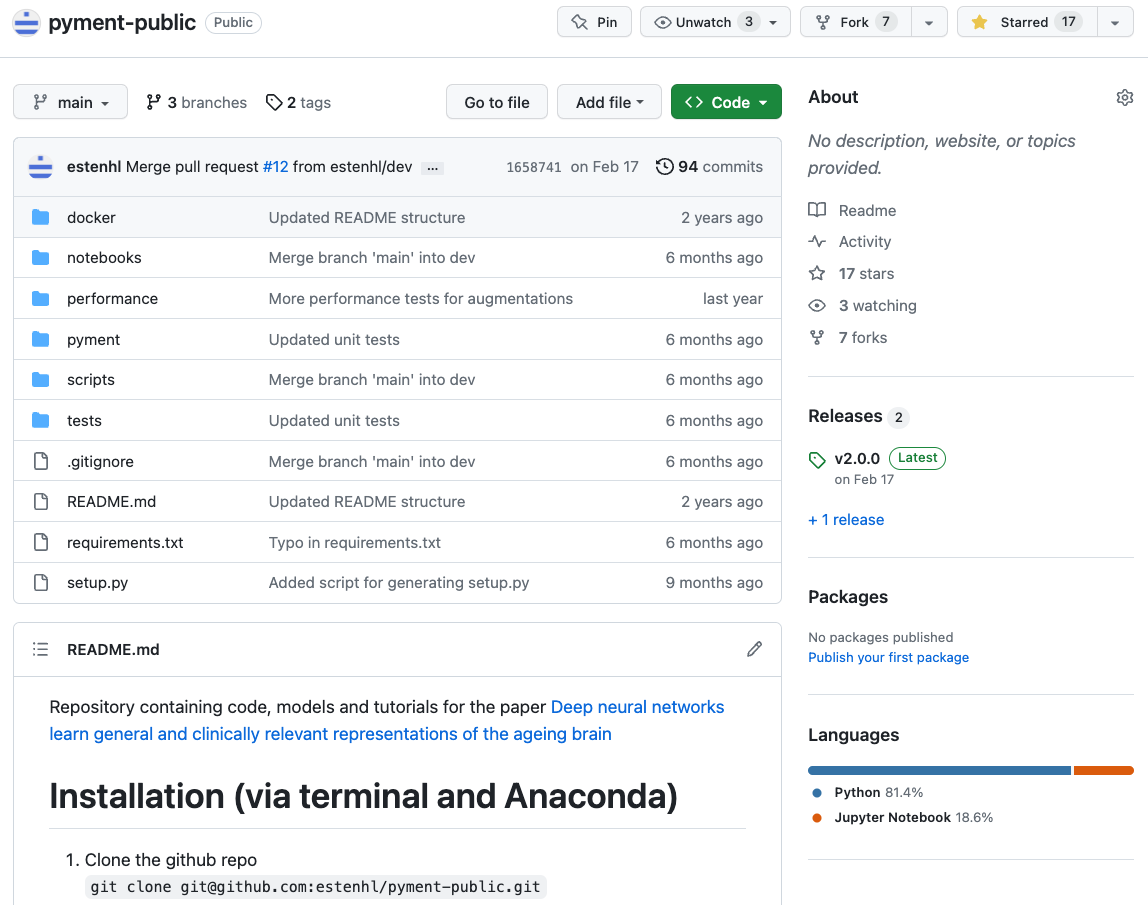
\includegraphics[width=7cm]{data/github.png}
			};
		\end{tikzpicture}
		\vfill
        Model freely available online
	\end{frame}

	\setbeamertemplate{footline}[genetic]
	\begin{frame}{Brain age: Associated SNPs}
		\centering
		\vfill
		\begin{tikzpicture}
			\node[inner sep=1pt, fill=white, draw=black] {
				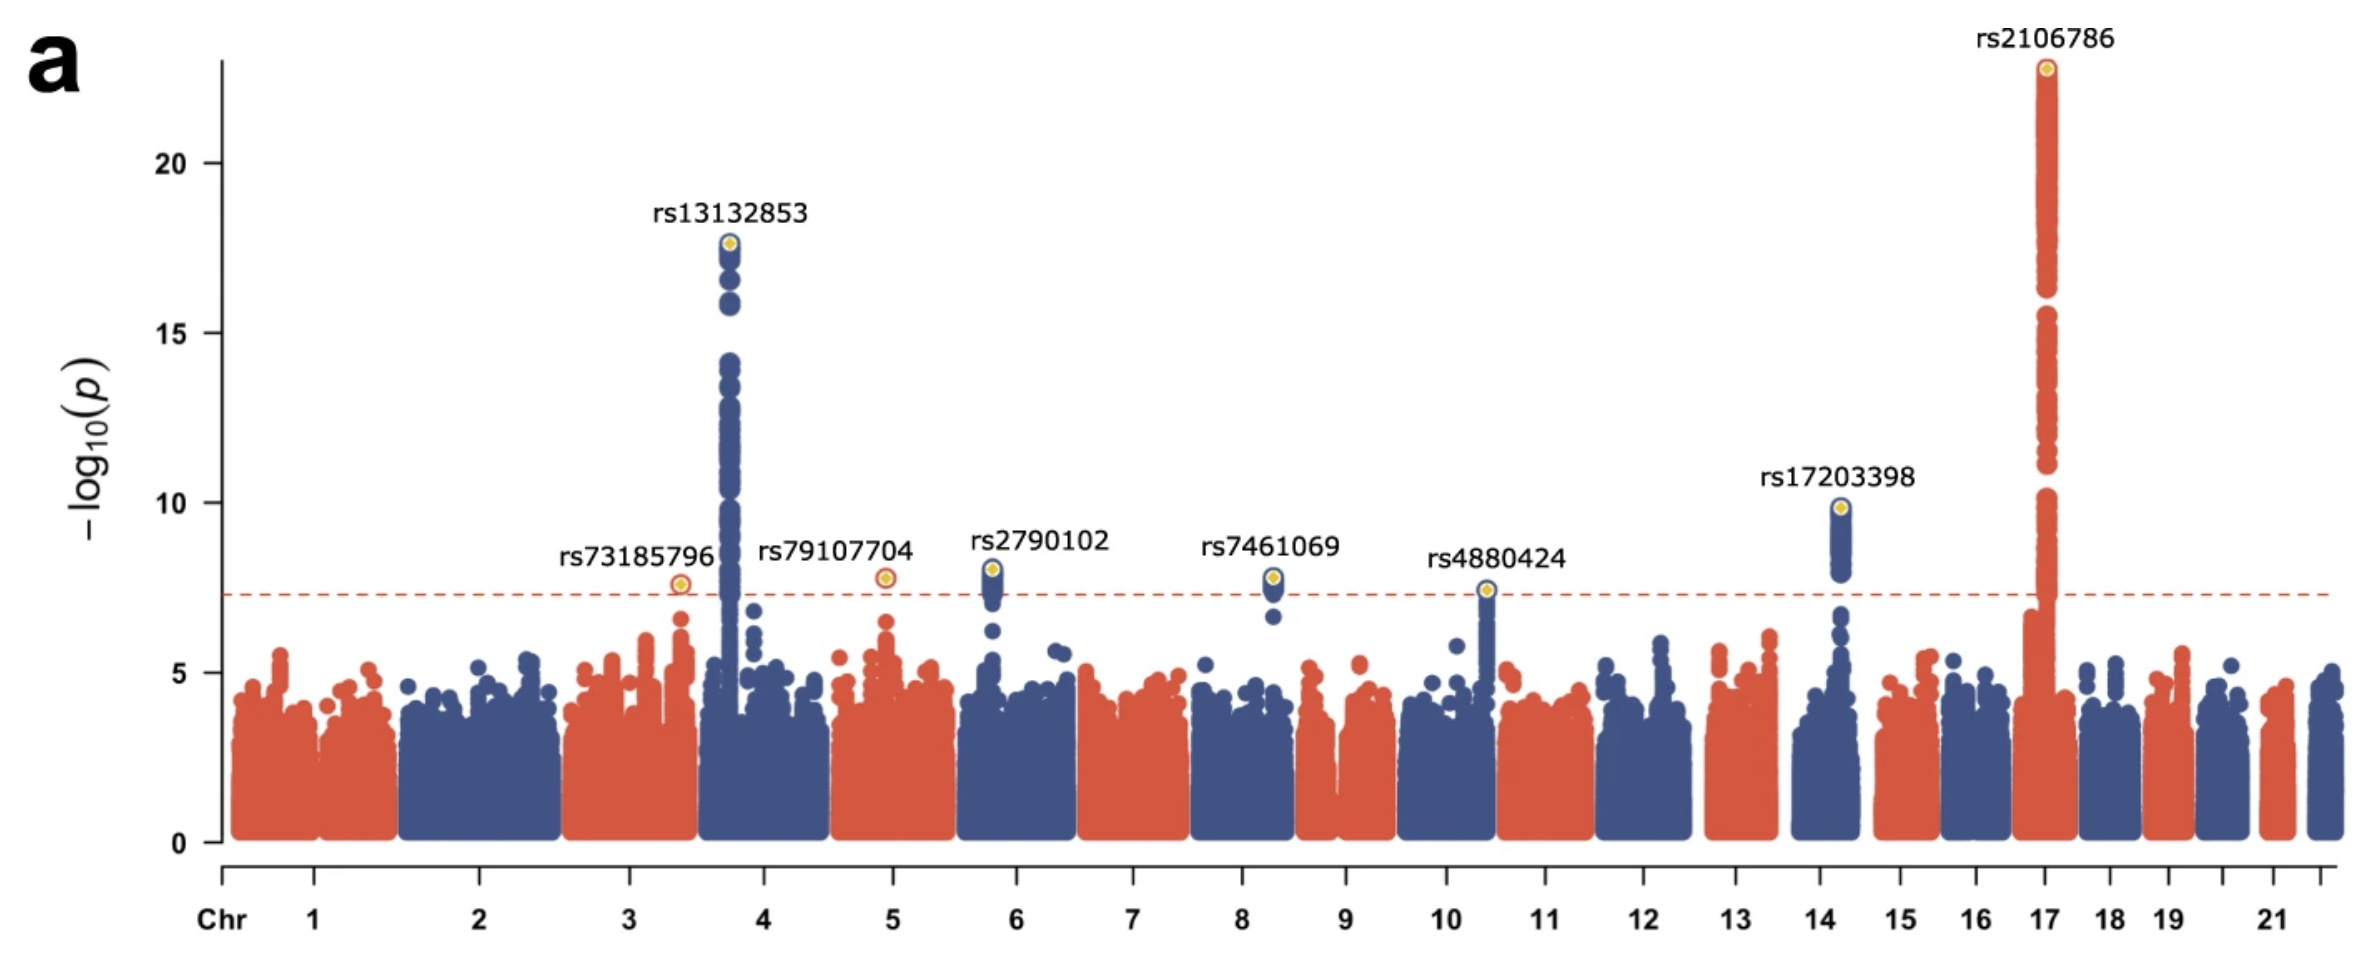
\includegraphics[width=10cm]{data/gwas.png}
			};
		\end{tikzpicture}
		\vfill
        8 SNPs significantly associated with differences in BAG, 7 novel
	\end{frame}

	\begin{frame}{Brain age: Associated genes}
		\centering
		\vfill
		\begin{tikzpicture}
			\node[inner sep=1pt, fill=white, draw=black] {
				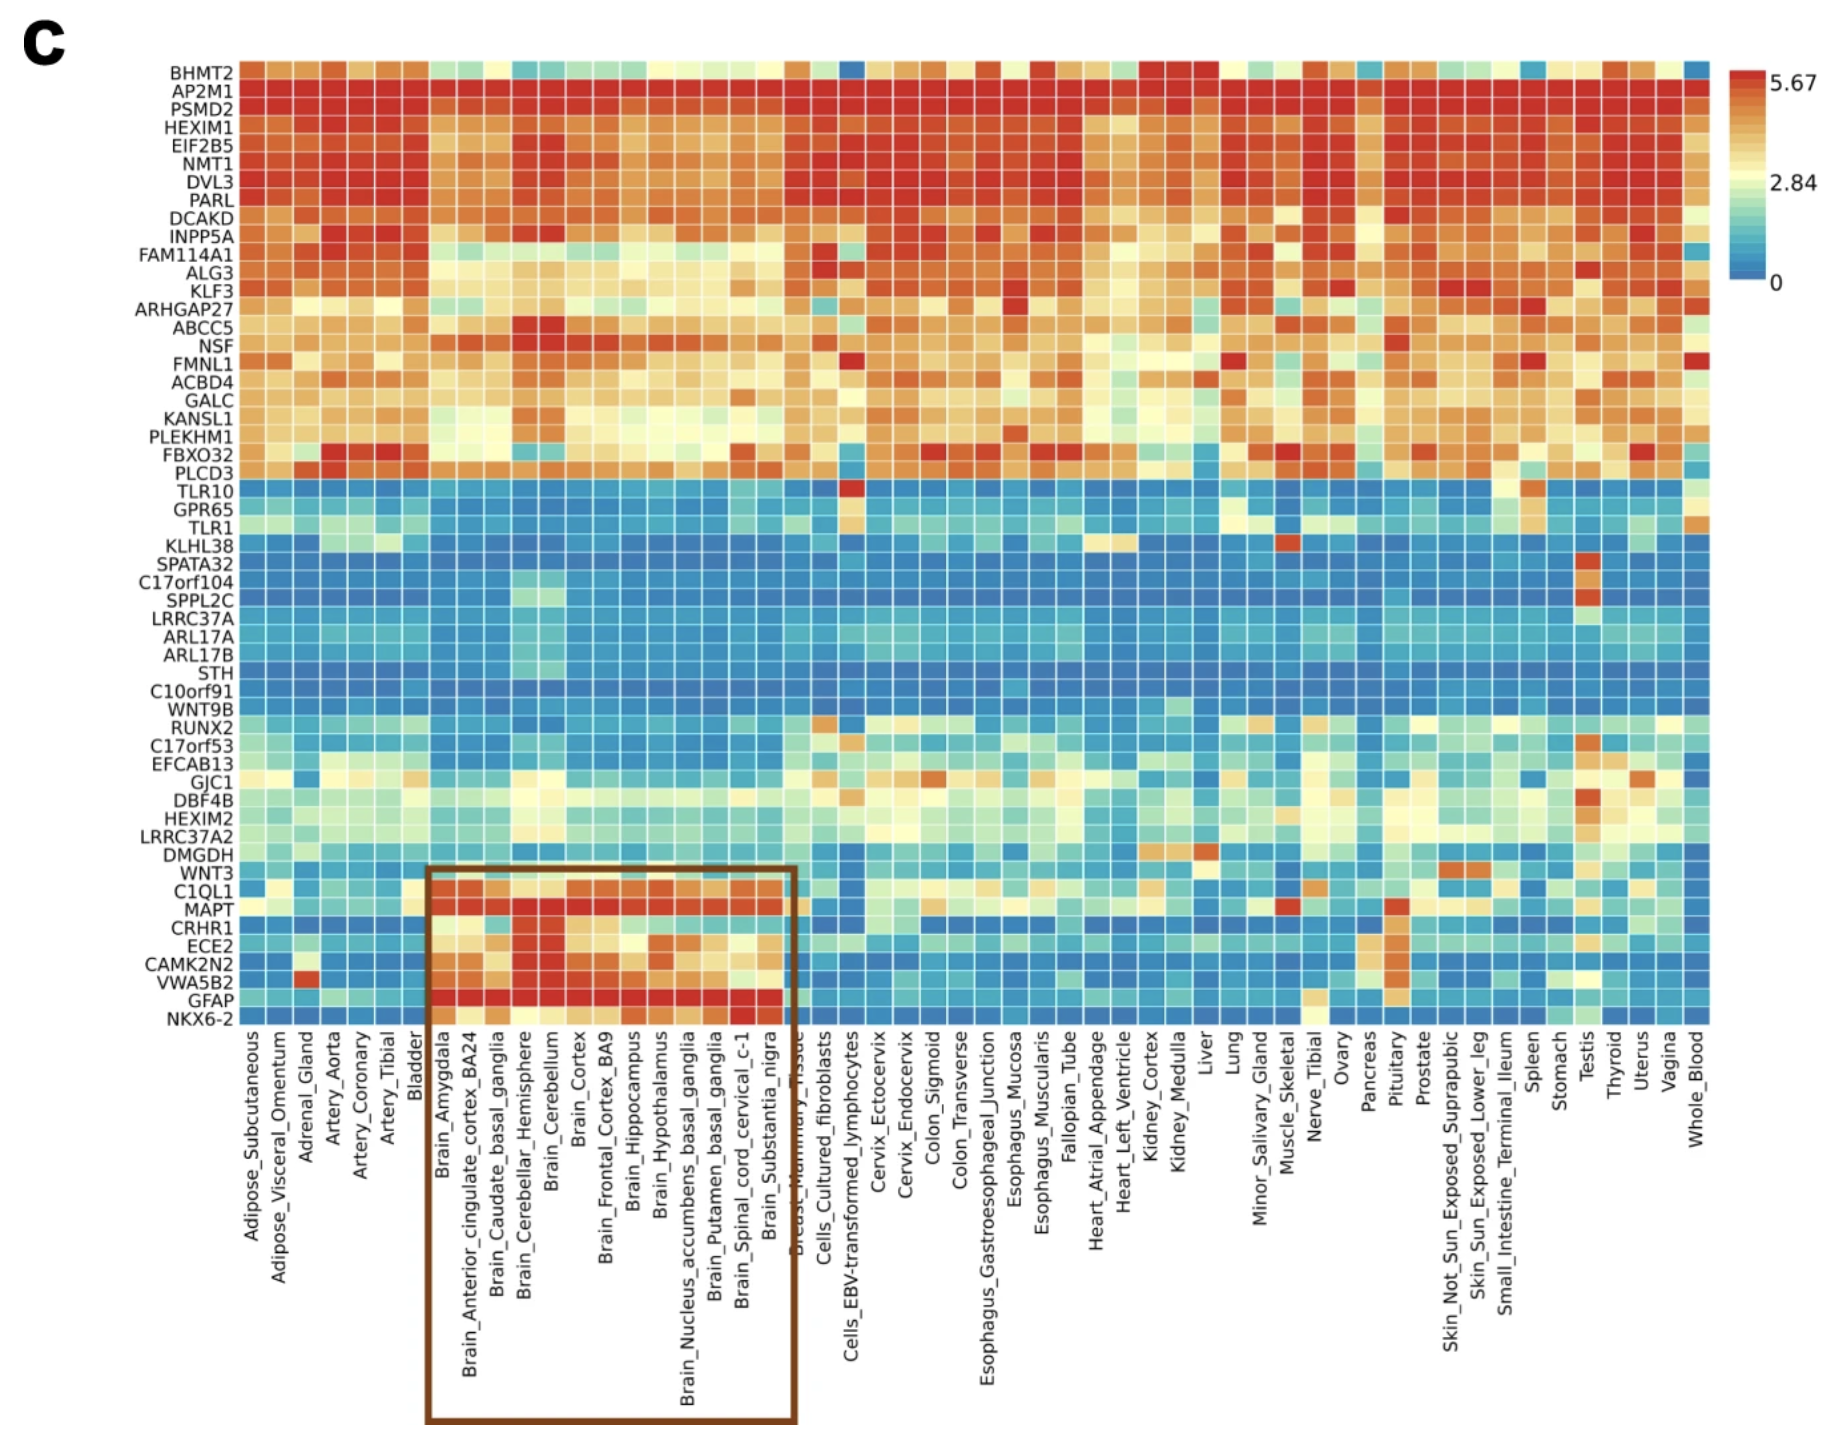
\includegraphics[width=8cm]{data/expression.png}
			};
		\end{tikzpicture}
		\vfill
        54 genes implicated, expressed in all tissue types
	\end{frame}

	\begin{frame}{Brain age: Genetic correlations}
		\centering
		\vfill
		\begin{tikzpicture}
			\node[inner sep=1pt, fill=white, draw=black] {
				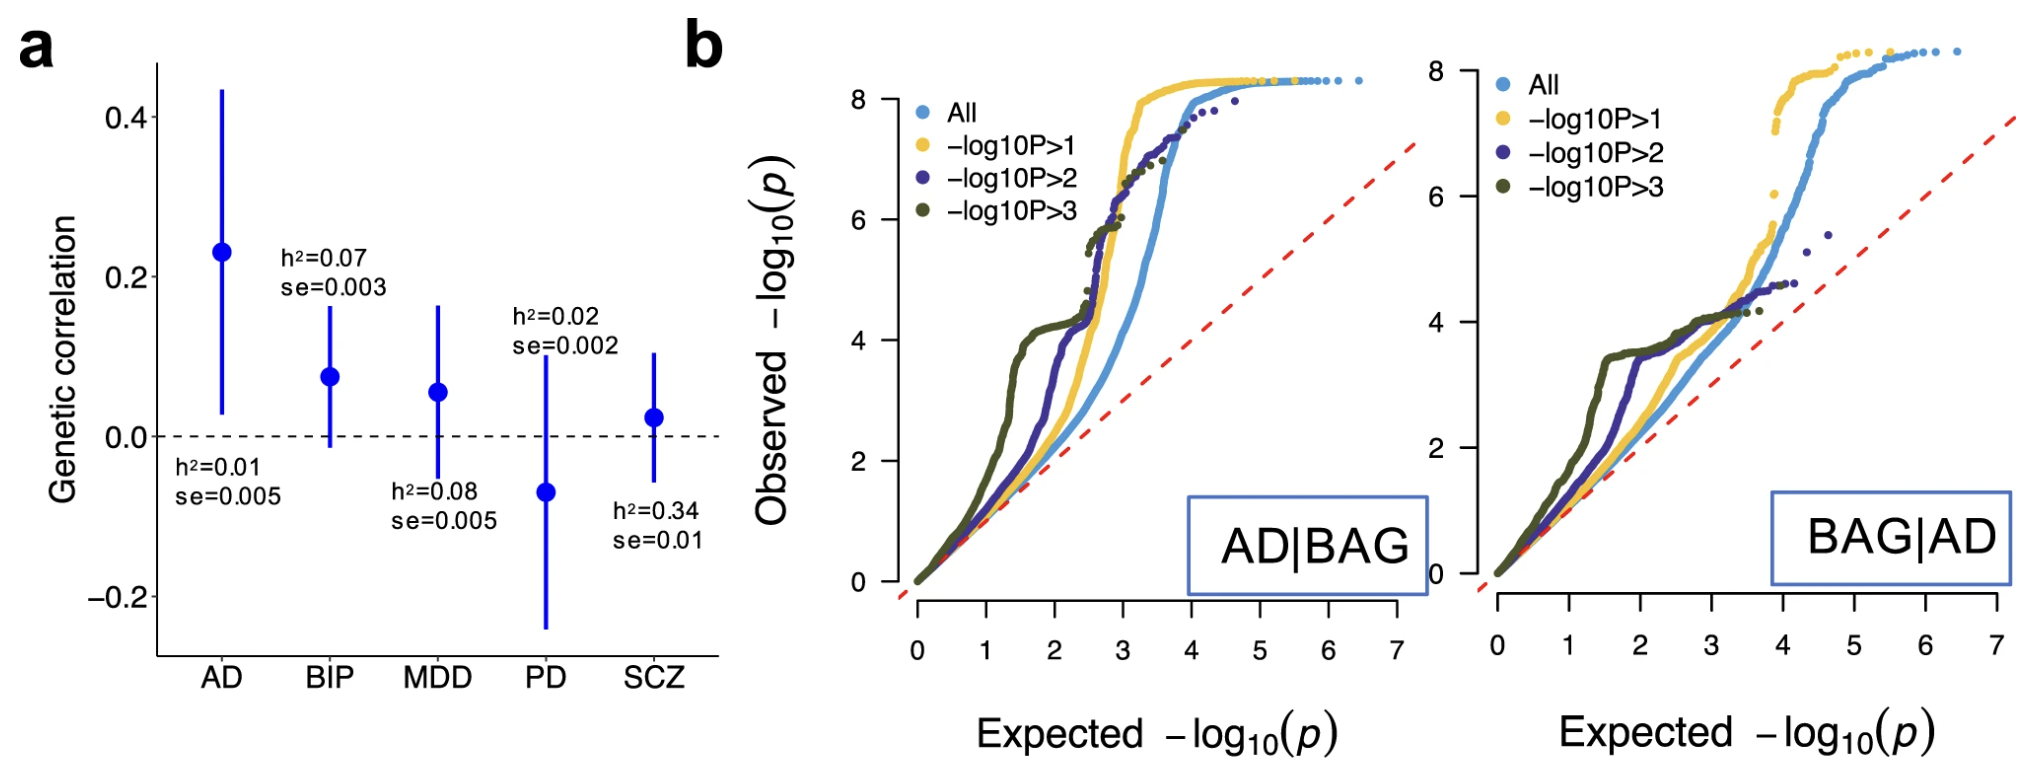
\includegraphics[width=10.5cm]{data/correlation.png}
			};
		\end{tikzpicture}
		\vfill
        Brain age gap (BAG) nominally genetically correlated with AD, no others
	\end{frame}

	\begin{frame}{Brain age: Causal effects}
		\centering
		\vfill
		\begin{tikzpicture}
			\node[inner sep=1pt, fill=white, draw=black] {
				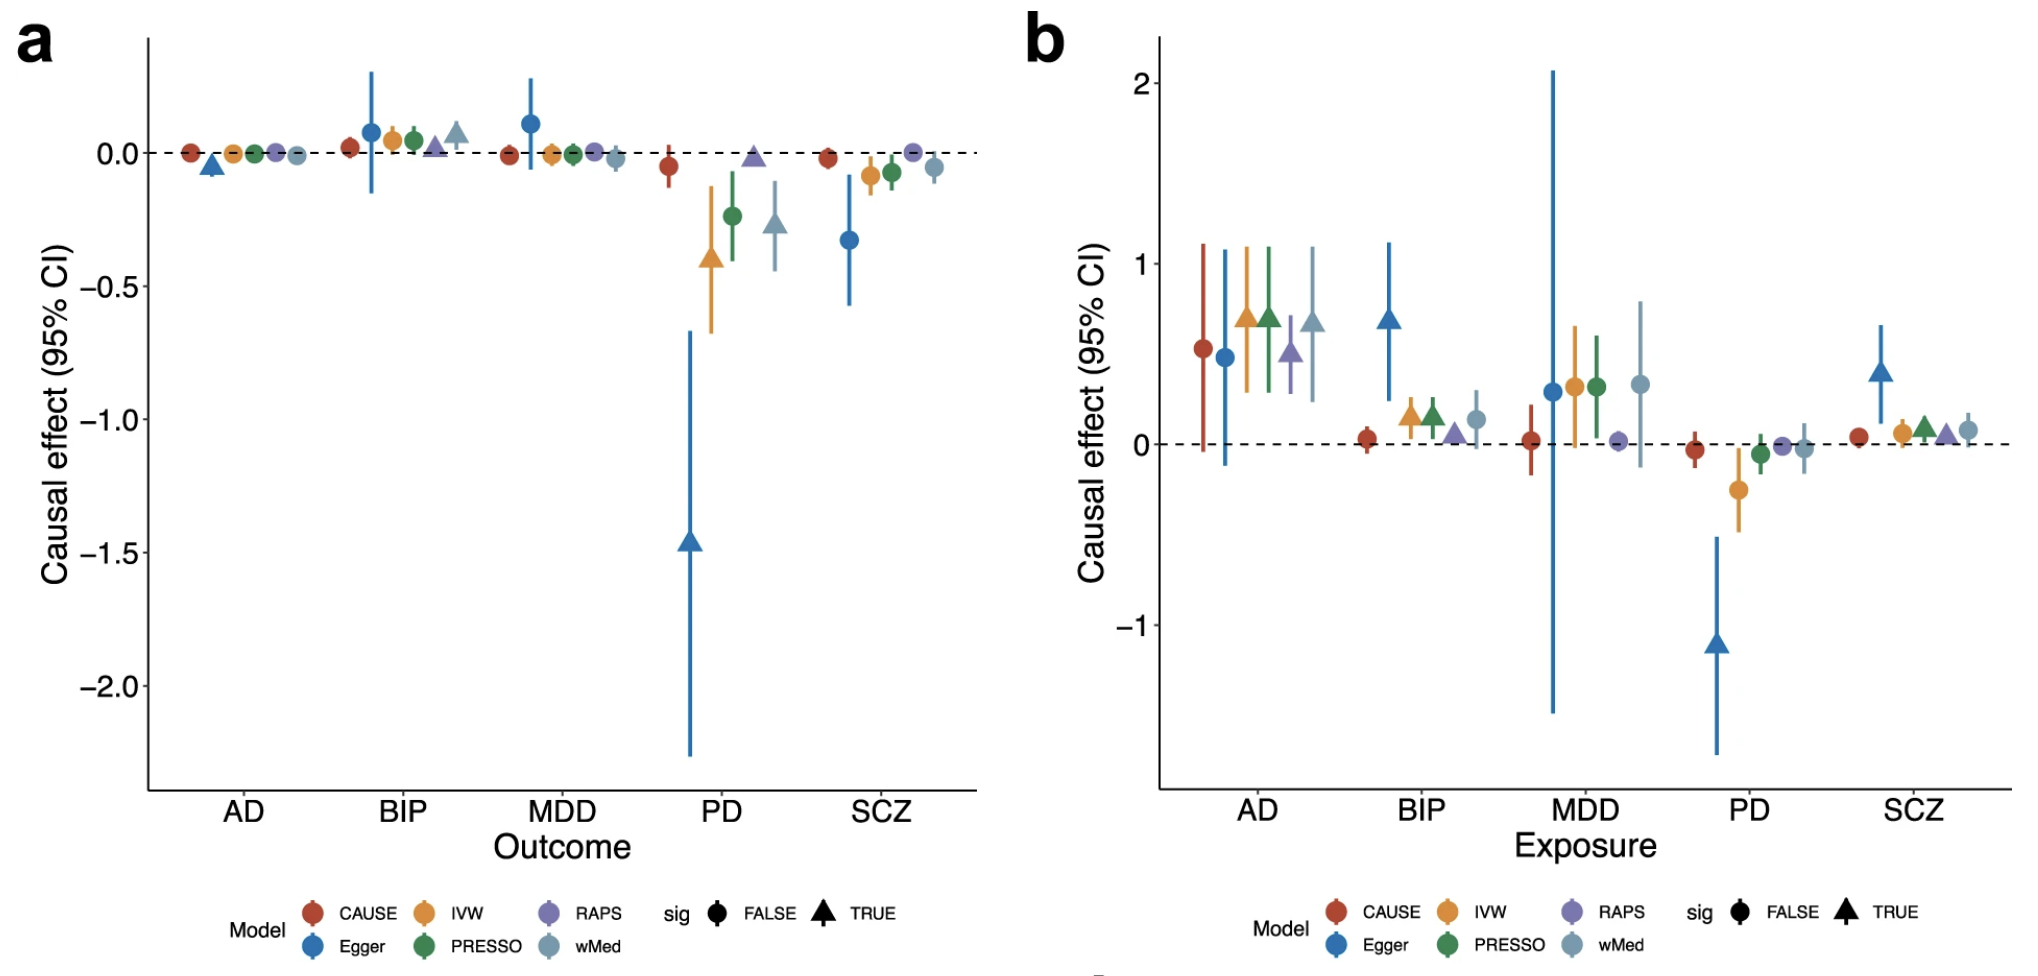
\includegraphics[width=10.5cm]{data/causality.png}
			};
		\end{tikzpicture}
		\vfill
        Evidence for causal effect of BAG on PD, BIP and AD on BAG
	\end{frame}

	\begin{frame}{Brain age: Causal effects}
		\centering
		\vfill
		\begin{tikzpicture}
			\node[inner sep=1pt, fill=white, draw=black] {
				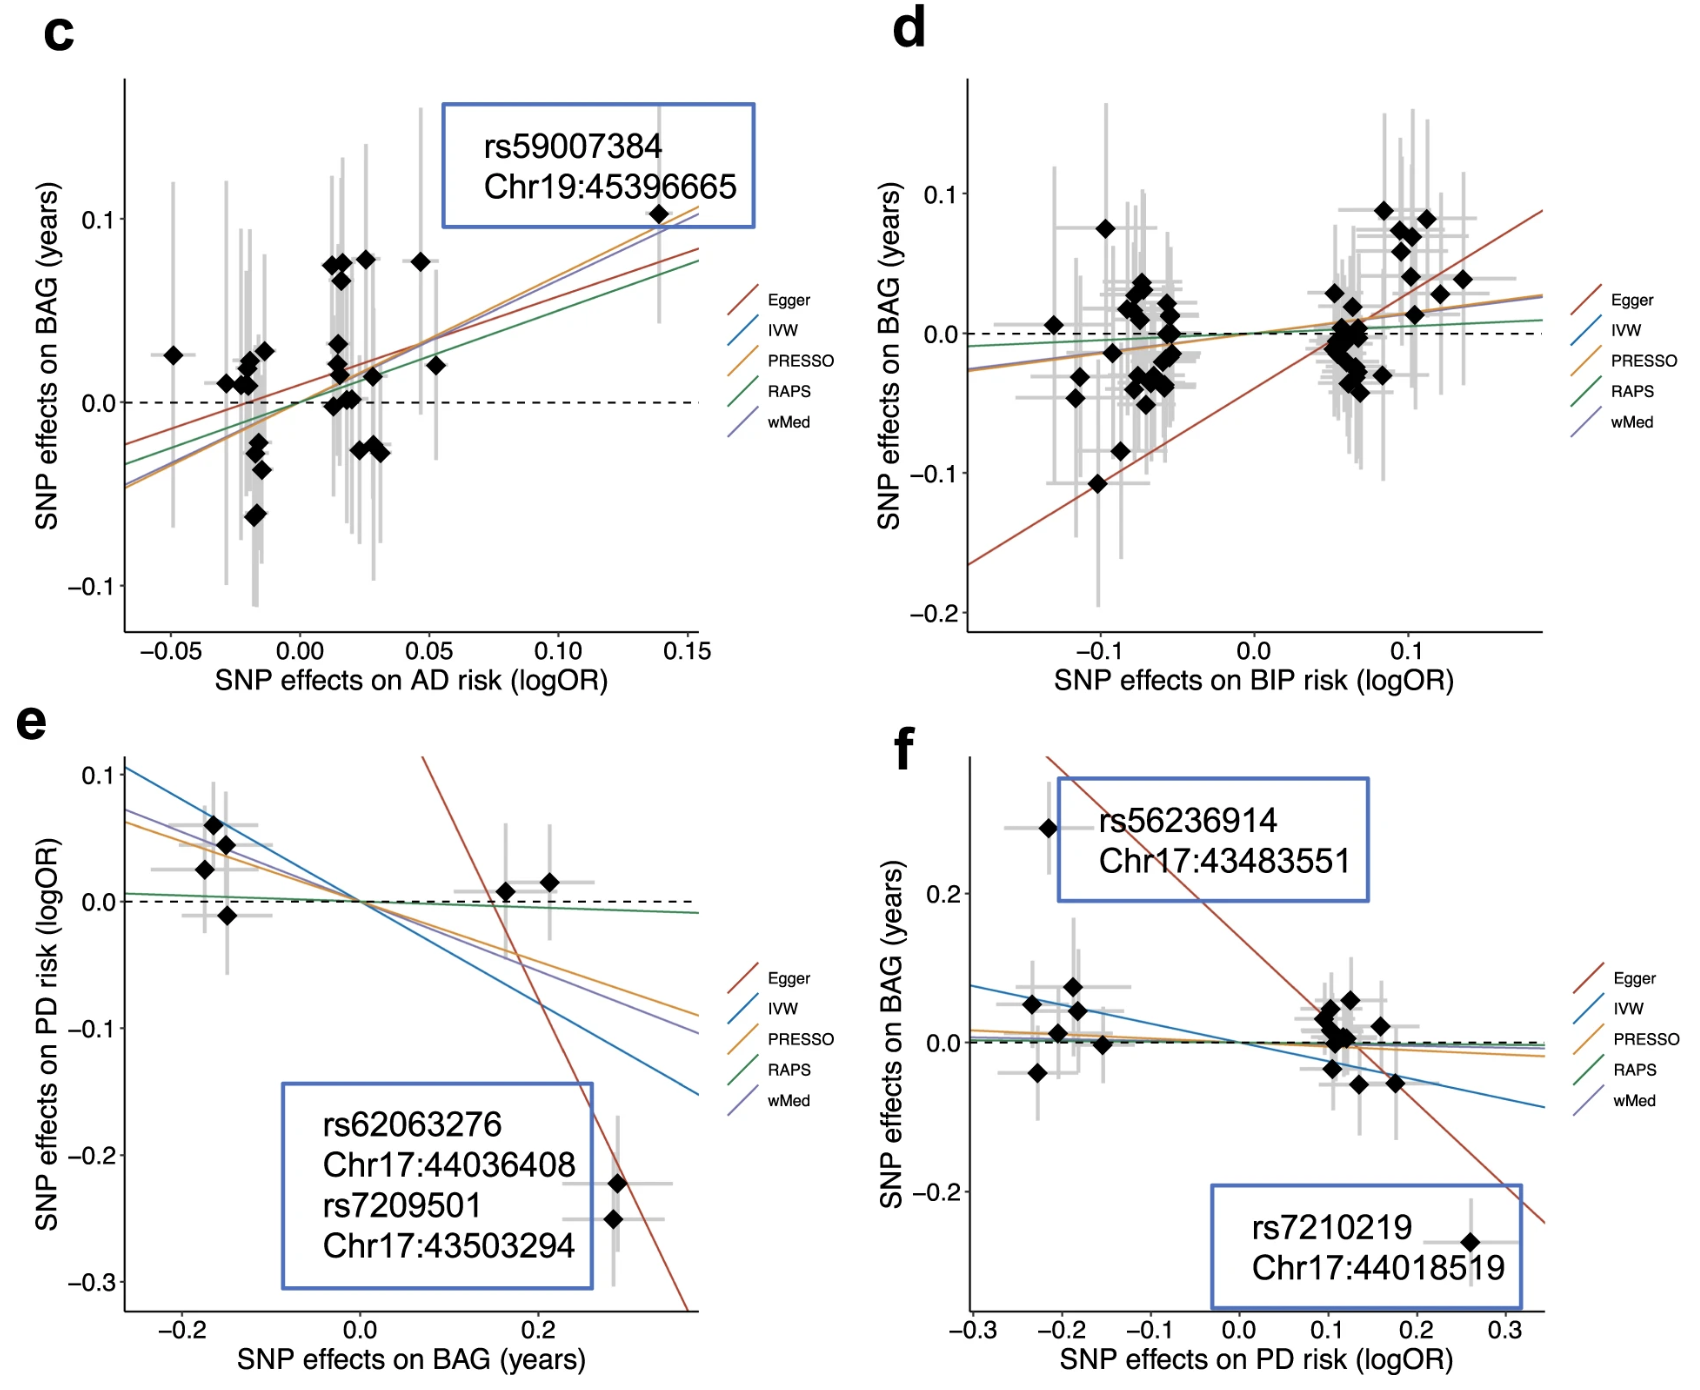
\includegraphics[width=8cm]{data/snp_effects.png}
			};
		\end{tikzpicture}
		\vfill
        BAG->PD driven by 2 SNPs (chr17), AD->BAG 1 SNP (APOE), horizontal pleiotropy identified for BIP->BAG
	\end{frame}

	\setbeamertemplate{footline}[didac]
	\begin{frame}{Brain age: Issues with interpretation}
		\centering
		\vfill
		\begin{tikzpicture}
			\node[inner sep=1pt, fill=white, draw=black] at (0, 0) {
				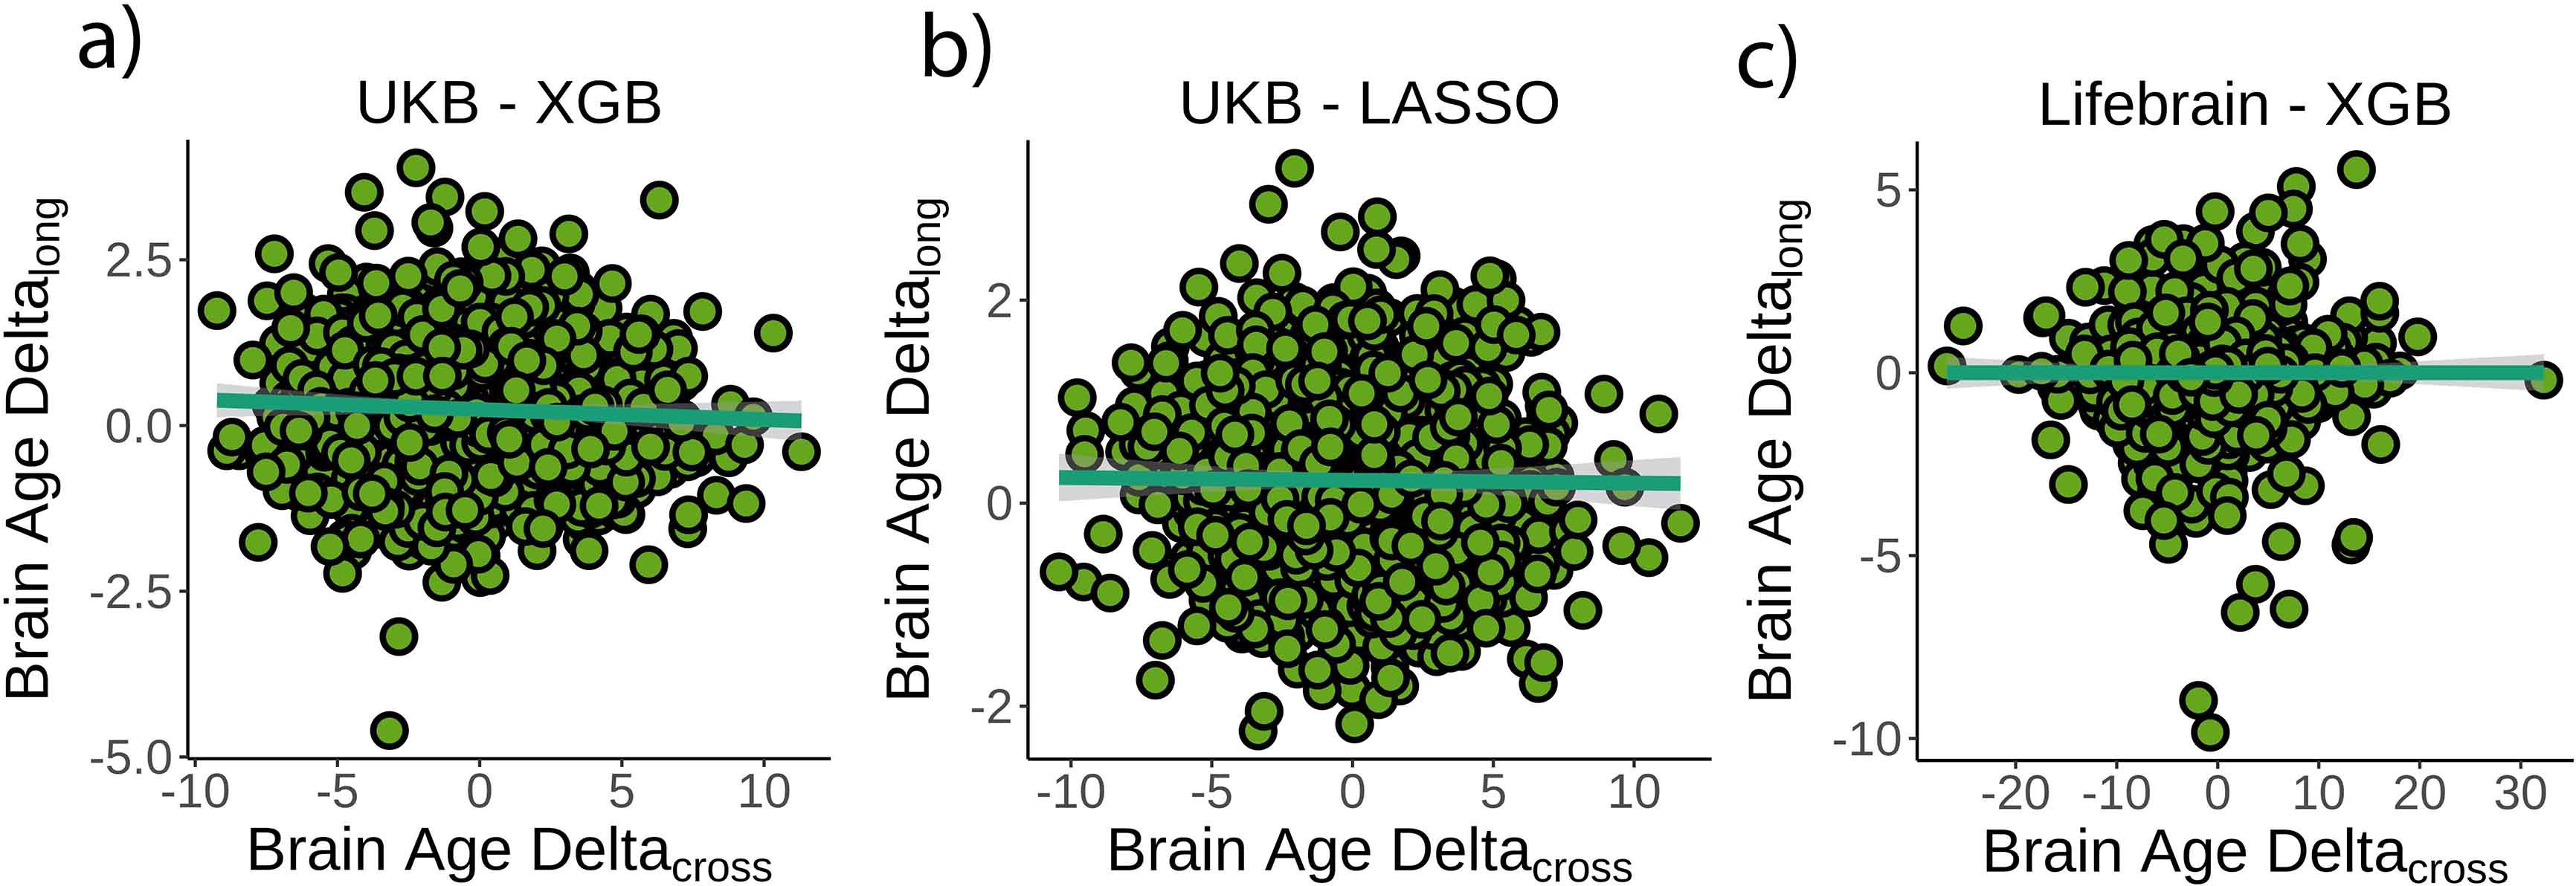
\includegraphics[width=5.5cm]{data/didac1.jpeg}
			};
			\node[inner sep=1pt, fill=white, draw=black] at (5.5, 0) {
				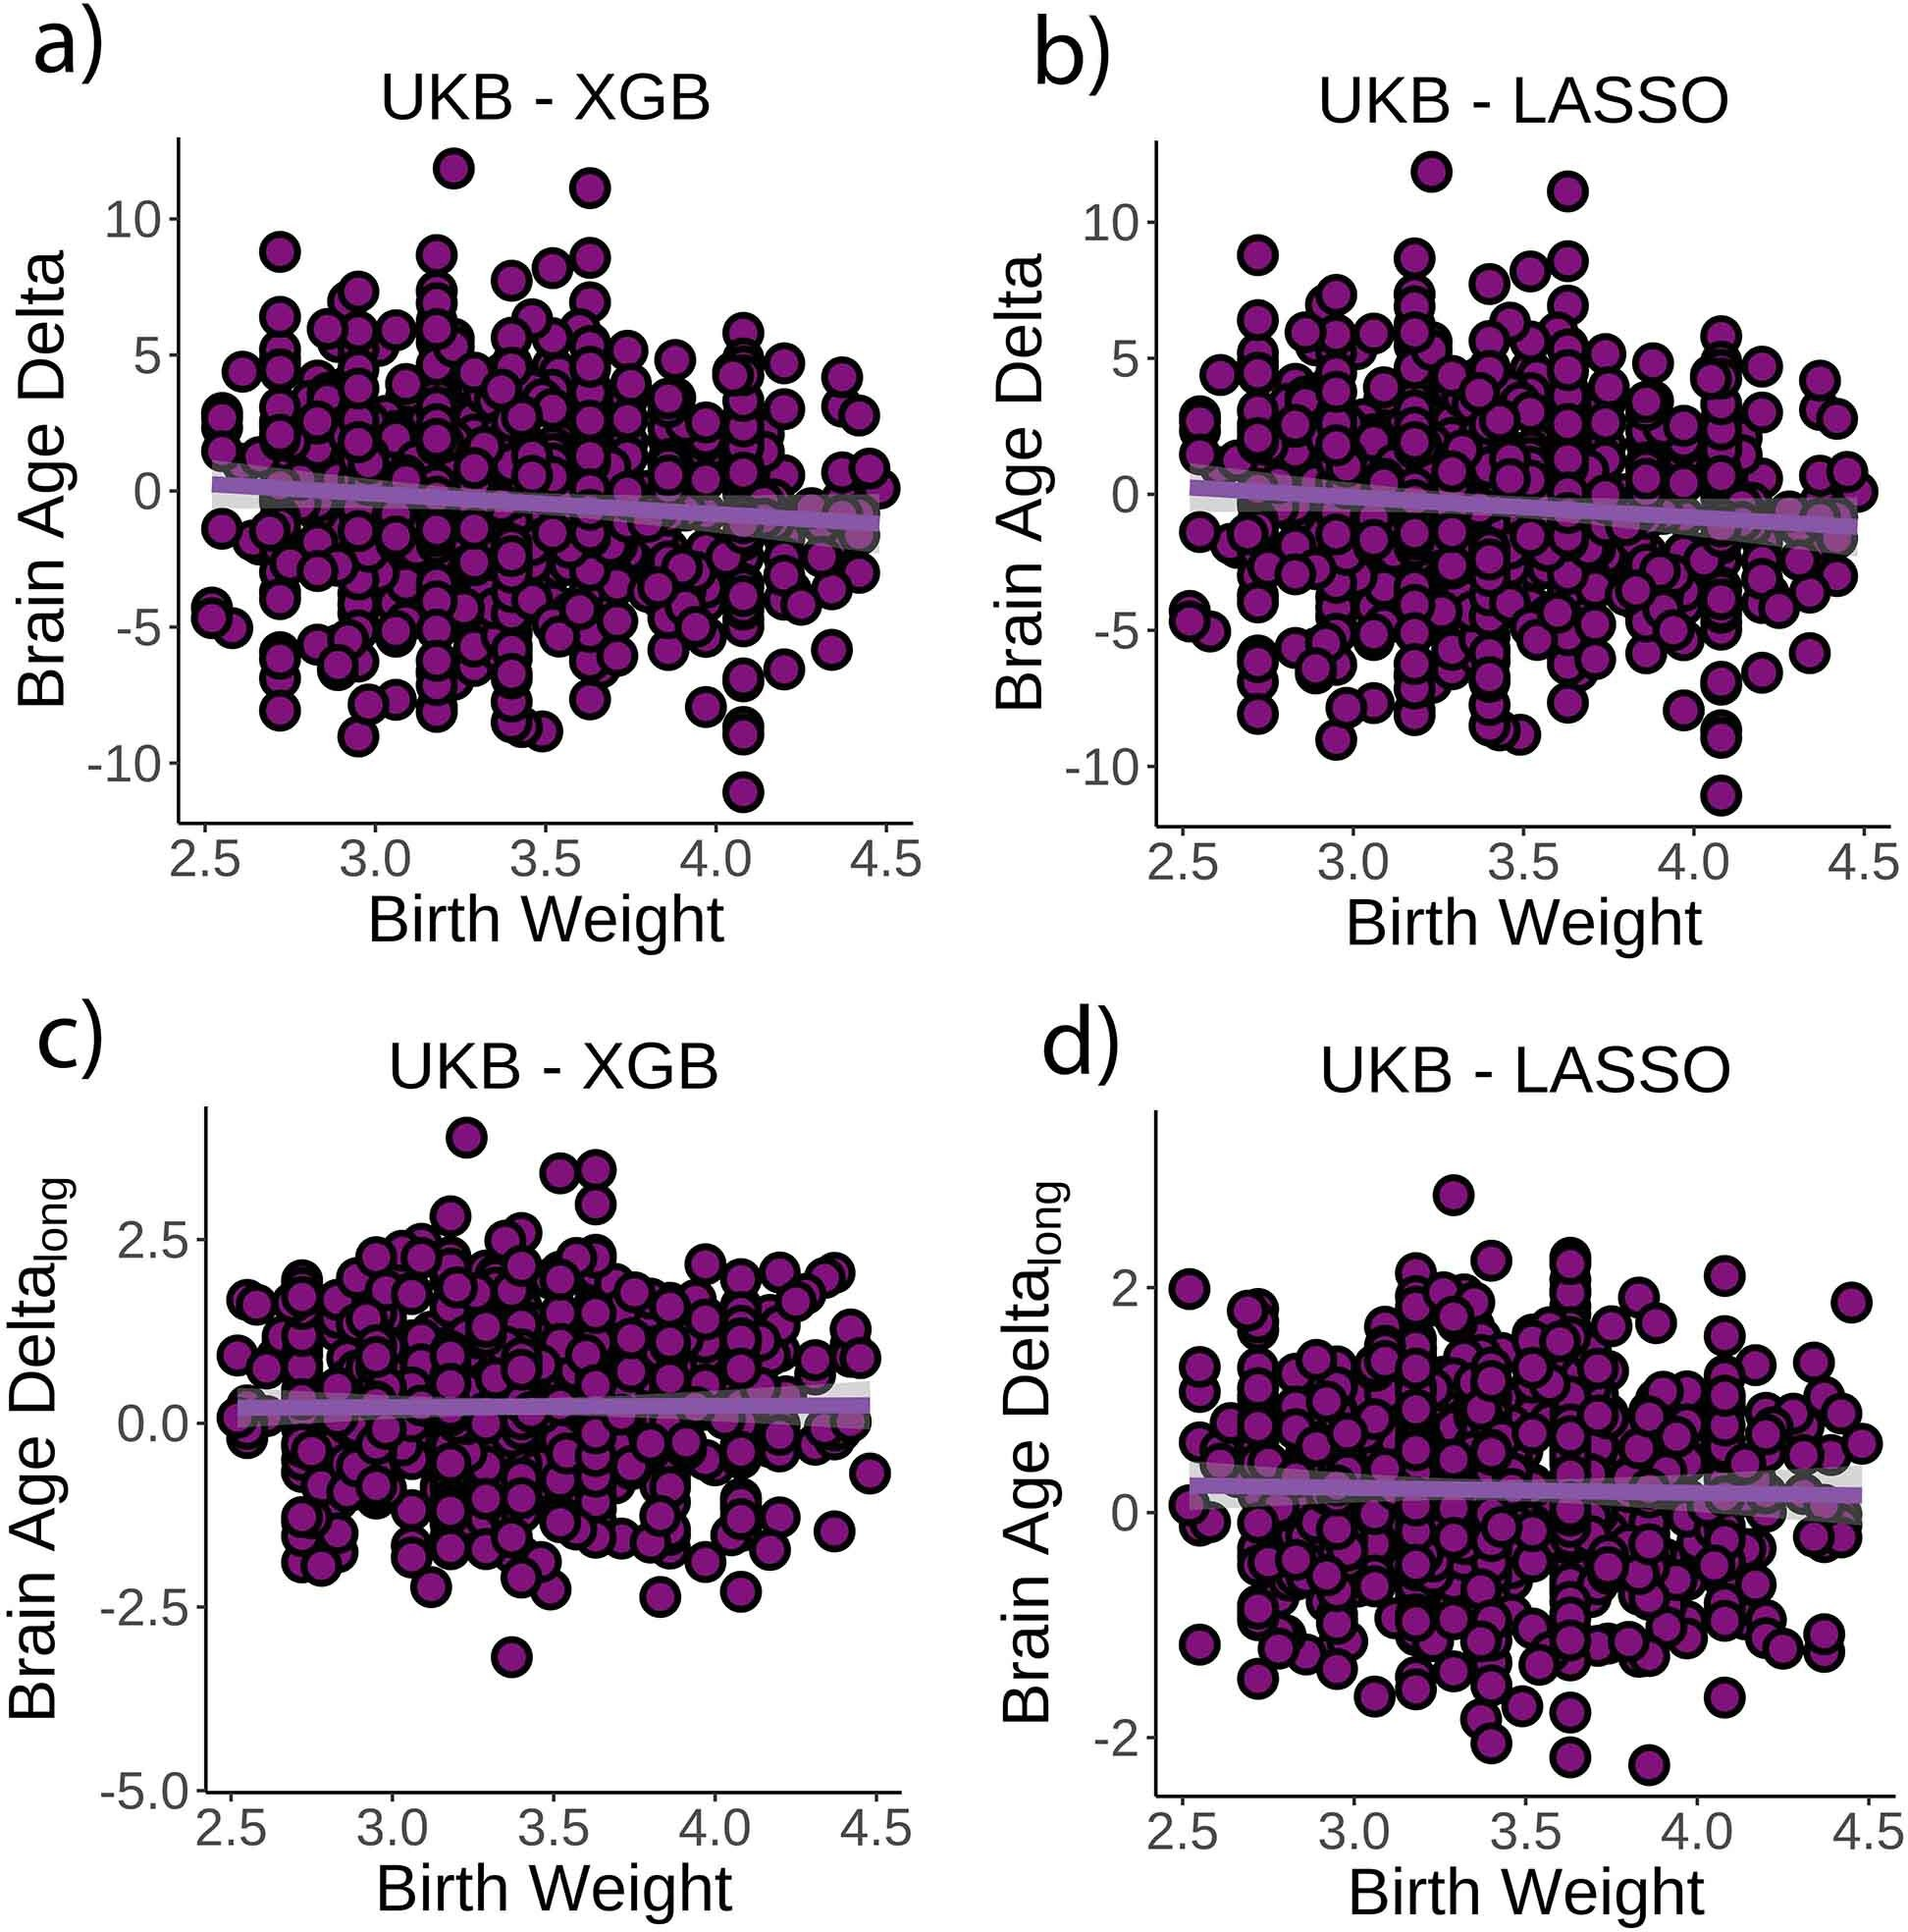
\includegraphics[width=4.5cm]{data/didac2.jpeg}
			};
		\end{tikzpicture}
		\vfill
        Cross-sectional BAG not associated with changes in BAG ($r^2=0.002$), but weakly with birth weight ($r^2=0.009$)
	\end{frame}

	\setbeamertemplate{footline}[max]
	\begin{frame}{Brain age: Issues with interpretation}
		\centering
		\vfill
		\begin{tikzpicture}
			\node[inner sep=1pt, fill=white, draw=black] {
				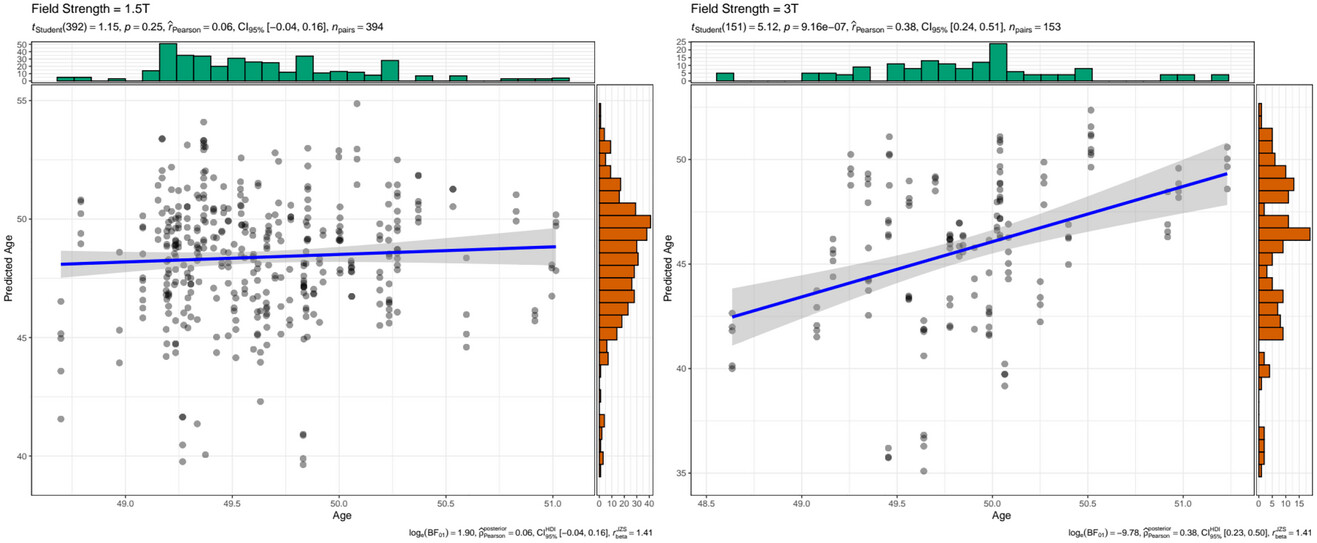
\includegraphics[width=10cm]{data/max.jpeg}
			};
		\end{tikzpicture}
		\vfill
        Within-subject variability in BAG associated with field strength (1.94 years mean difference)
	\end{frame}

    \setbeamertemplate{footline}[madde]
	\begin{frame}{Brain age: Association with pubertal development}
		\centering
		\vfill
		\begin{tikzpicture}
			\node[inner sep=1pt, fill=white, draw=black] {
				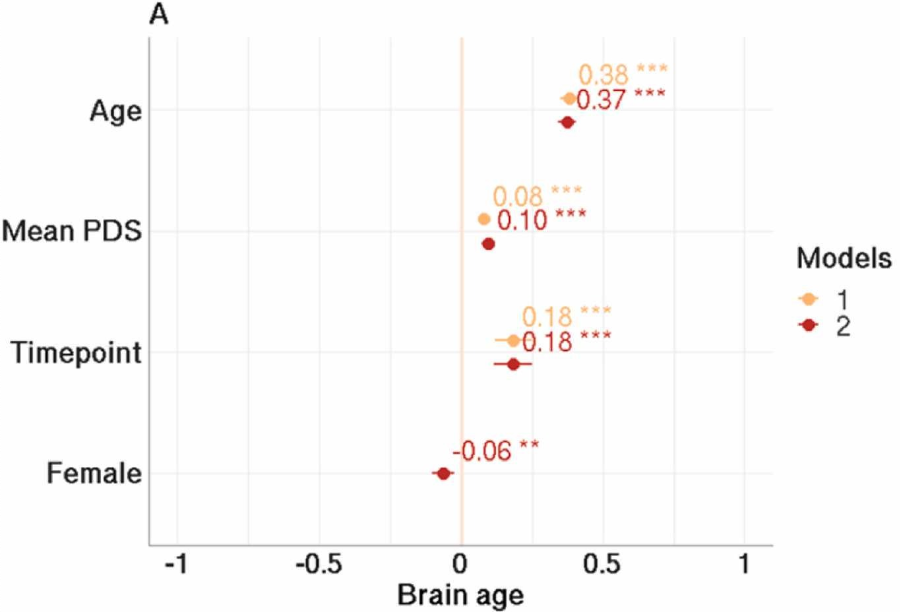
\includegraphics[width=7cm]{data/madelene.png}
			};
		\end{tikzpicture}
		\vfill
        Higher brain age associated with advanced pubertal development
	\end{frame}

	\setbeamertemplate{footline}[explainable]
	\begin{frame}{Brain age: Updated sample}
        \centering
        \vfill
		\begin{tikzpicture}
			\pgfplotstableread[col sep=comma]{/Users/esten/phd/papers/2023-explainable-brain-age/data/full_data_distributions.csv}\data
			\begin{axis}[
				width=0.8\textwidth,
				height=0.85\textwidth,
				xmin=0,
				xmax=100,
				ytick=\empty,
				axis x line=middle,
				axis y line=none,
				xtick={10,20,30,40,50,60,70,80},
				x axis line style={|-stealth},
				clip=false
			]
				\addplot[
					name path=zero,
				] coordinates {(0,0) (100,0)};
				\addplot [
					draw=none,
					line width=0pt,
					name path={female_ds002424},
				] table [
					x=age,
					y expr=1 * \thisrow{female_ds002424}
				]{\data};
				\addplot [
					draw=none,
					line width=0pt,
					name path={female_HBN},
				] table [
					x=age,
					y expr=1 * \thisrow{female_HBN}
				]{\data};
				\addplot [
					draw=none,
					line width=0pt,
					name path={female_ABCD},
				] table [
					x=age,
					y expr=1 * \thisrow{female_ABCD}
				]{\data};
				\addplot [
					draw=none,
					line width=0pt,
					name path={female_QTAB},
				] table [
					x=age,
					y expr=1 * \thisrow{female_QTAB}
				]{\data};
				\addplot [
					draw=none,
					line width=0pt,
					name path={female_PING},
				] table [
					x=age,
					y expr=1 * \thisrow{female_PING}
				]{\data};
				\addplot [
					draw=none,
					line width=0pt,
					name path={female_ADHD200},
				] table [
					x=age,
					y expr=1 * \thisrow{female_ADHD200}
				]{\data};
				\addplot [
					draw=none,
					line width=0pt,
					name path={female_PNC},
				] table [
					x=age,
					y expr=1 * \thisrow{female_PNC}
				]{\data};
				\addplot [
					draw=none,
					line width=0pt,
					name path={female_ABIDE II},
				] table [
					x=age,
					y expr=1 * \thisrow{female_ABIDE II}
				]{\data};
				\addplot [
					draw=none,
					line width=0pt,
					name path={female_ds000119},
				] table [
					x=age,
					y expr=1 * \thisrow{female_ds000119}
				]{\data};
				\addplot [
					draw=none,
					line width=0pt,
					name path={female_ABIDE I},
				] table [
					x=age,
					y expr=1 * \thisrow{female_ABIDE I}
				]{\data};
				\addplot [
					draw=none,
					line width=0pt,
					name path={female_BRAINMINT},
				] table [
					x=age,
					y expr=1 * \thisrow{female_BRAINMINT}
				]{\data};
				\addplot [
					draw=none,
					line width=0pt,
					name path={female_SLIM},
				] table [
					x=age,
					y expr=1 * \thisrow{female_SLIM}
				]{\data};
				\addplot [
					draw=none,
					line width=0pt,
					name path={female_QTIM},
				] table [
					x=age,
					y expr=1 * \thisrow{female_QTIM}
				]{\data};
				\addplot [
					draw=none,
					line width=0pt,
					name path={female_Beijing},
				] table [
					x=age,
					y expr=1 * \thisrow{female_Beijing}
				]{\data};
				\addplot [
					draw=none,
					line width=0pt,
					name path={female_AOMIC-PIOP2},
				] table [
					x=age,
					y expr=1 * \thisrow{female_AOMIC-PIOP2}
				]{\data};
				\addplot [
					draw=none,
					line width=0pt,
					name path={female_ds000202},
				] table [
					x=age,
					y expr=1 * \thisrow{female_ds000202}
				]{\data};
				\addplot [
					draw=none,
					line width=0pt,
					name path={female_AOMIC-PIOP1},
				] table [
					x=age,
					y expr=1 * \thisrow{female_AOMIC-PIOP1}
				]{\data};
				\addplot [
					draw=none,
					line width=0pt,
					name path={female_AOMIC-ID1000},
				] table [
					x=age,
					y expr=1 * \thisrow{female_AOMIC-ID1000}
				]{\data};
				\addplot [
					draw=none,
					line width=0pt,
					name path={female_CoRR},
				] table [
					x=age,
					y expr=1 * \thisrow{female_CoRR}
				]{\data};
				\addplot [
					draw=none,
					line width=0pt,
					name path={female_HCP},
				] table [
					x=age,
					y expr=1 * \thisrow{female_HCP}
				]{\data};
				\addplot [
					draw=none,
					line width=0pt,
					name path={female_FCON1000},
				] table [
					x=age,
					y expr=1 * \thisrow{female_FCON1000}
				]{\data};
				\addplot [
					draw=none,
					line width=0pt,
					name path={female_ds000171},
				] table [
					x=age,
					y expr=1 * \thisrow{female_ds000171}
				]{\data};
				\addplot [
					draw=none,
					line width=0pt,
					name path={female_TOP},
				] table [
					x=age,
					y expr=1 * \thisrow{female_TOP}
				]{\data};
				\addplot [
					draw=none,
					line width=0pt,
					name path={female_SCZ-Z},
				] table [
					x=age,
					y expr=1 * \thisrow{female_SCZ-Z}
				]{\data};
				\addplot [
					draw=none,
					line width=0pt,
					name path={female_NIMH},
				] table [
					x=age,
					y expr=1 * \thisrow{female_NIMH}
				]{\data};
				\addplot [
					draw=none,
					line width=0pt,
					name path={female_NKI-RS},
				] table [
					x=age,
					y expr=1 * \thisrow{female_NKI-RS}
				]{\data};
				\addplot [
					draw=none,
					line width=0pt,
					name path={female_MPI-LEMON},
				] table [
					x=age,
					y expr=1 * \thisrow{female_MPI-LEMON}
				]{\data};
				\addplot [
					draw=none,
					line width=0pt,
					name path={female_ds003592},
				] table [
					x=age,
					y expr=1 * \thisrow{female_ds003592}
				]{\data};
				\addplot [
					draw=none,
					line width=0pt,
					name path={female_ds004302},
				] table [
					x=age,
					y expr=1 * \thisrow{female_ds004302}
				]{\data};
				\addplot [
					draw=none,
					line width=0pt,
					name path={female_ds000222},
				] table [
					x=age,
					y expr=1 * \thisrow{female_ds000222}
				]{\data};
				\addplot [
					draw=none,
					line width=0pt,
					name path={female_SALD},
				] table [
					x=age,
					y expr=1 * \thisrow{female_SALD}
				]{\data};
				\addplot [
					draw=none,
					line width=0pt,
					name path={female_IXI},
				] table [
					x=age,
					y expr=1 * \thisrow{female_IXI}
				]{\data};
				\addplot [
					draw=none,
					line width=0pt,
					name path={female_DLBS},
				] table [
					x=age,
					y expr=1 * \thisrow{female_DLBS}
				]{\data};
				\addplot [
					draw=none,
					line width=0pt,
					name path={female_Cam-CAN},
				] table [
					x=age,
					y expr=1 * \thisrow{female_Cam-CAN}
				]{\data};
				\addplot [
					draw=none,
					line width=0pt,
					name path={female_StrokeMRI},
				] table [
					x=age,
					y expr=1 * \thisrow{female_StrokeMRI}
				]{\data};
				\addplot [
					draw=none,
					line width=0pt,
					name path={female_PPMI},
				] table [
					x=age,
					y expr=1 * \thisrow{female_PPMI}
				]{\data};
				\addplot [
					draw=none,
					line width=0pt,
					name path={female_UKBB},
				] table [
					x=age,
					y expr=1 * \thisrow{female_UKBB}
				]{\data};
				\addplot [
					draw=none,
					line width=0pt,
					name path={female_Tao-Wu},
				] table [
					x=age,
					y expr=1 * \thisrow{female_Tao-Wu}
				]{\data};
				\addplot [
					draw=none,
					line width=0pt,
					name path={female_ds000245},
				] table [
					x=age,
					y expr=1 * \thisrow{female_ds000245}
				]{\data};
				\addplot [
					draw=none,
					line width=0pt,
					name path={female_OASIS3},
				] table [
					x=age,
					y expr=1 * \thisrow{female_OASIS3}
				]{\data};
				\addplot [
					draw=none,
					line width=0pt,
					name path={female_Demgen},
				] table [
					x=age,
					y expr=1 * \thisrow{female_Demgen}
				]{\data};
				\addplot [
					draw=none,
					line width=0pt,
					name path={female_NEUROCON},
				] table [
					x=age,
					y expr=1 * \thisrow{female_NEUROCON}
				]{\data};
				\addplot [
					draw=none,
					line width=0pt,
					name path={female_MIRIAD},
				] table [
					x=age,
					y expr=1 * \thisrow{female_MIRIAD}
				]{\data};
				\addplot [
					draw=none,
					line width=0pt,
					name path={female_ds004392},
				] table [
					x=age,
					y expr=1 * \thisrow{female_ds004392}
				]{\data};
				\addplot [
					draw=none,
					line width=0pt,
					name path={female_AIBL},
				] table [
					x=age,
					y expr=1 * \thisrow{female_AIBL}
				]{\data};
				\addplot [
					draw=none,
					line width=0pt,
					name path={female_ANM},
				] table [
					x=age,
					y expr=1 * \thisrow{female_ANM}
				]{\data};
				\addplot [
					draw=none,
					line width=0pt,
					name path={female_ADNI},
				] table [
					x=age,
					y expr=1 * \thisrow{female_ADNI}
				]{\data};
				\addplot [
					draw=none,
					line width=0pt,
					name path={male_ds002424},
				] table [
					x=age,
					y expr=-1 * \thisrow{male_ds002424}
				]{\data};
				\addplot [
					draw=none,
					line width=0pt,
					name path={male_HBN},
				] table [
					x=age,
					y expr=-1 * \thisrow{male_HBN}
				]{\data};
				\addplot [
					draw=none,
					line width=0pt,
					name path={male_ABCD},
				] table [
					x=age,
					y expr=-1 * \thisrow{male_ABCD}
				]{\data};
				\addplot [
					draw=none,
					line width=0pt,
					name path={male_QTAB},
				] table [
					x=age,
					y expr=-1 * \thisrow{male_QTAB}
				]{\data};
				\addplot [
					draw=none,
					line width=0pt,
					name path={male_PING},
				] table [
					x=age,
					y expr=-1 * \thisrow{male_PING}
				]{\data};
				\addplot [
					draw=none,
					line width=0pt,
					name path={male_ADHD200},
				] table [
					x=age,
					y expr=-1 * \thisrow{male_ADHD200}
				]{\data};
				\addplot [
					draw=none,
					line width=0pt,
					name path={male_PNC},
				] table [
					x=age,
					y expr=-1 * \thisrow{male_PNC}
				]{\data};
				\addplot [
					draw=none,
					line width=0pt,
					name path={male_ABIDE II},
				] table [
					x=age,
					y expr=-1 * \thisrow{male_ABIDE II}
				]{\data};
				\addplot [
					draw=none,
					line width=0pt,
					name path={male_ds000119},
				] table [
					x=age,
					y expr=-1 * \thisrow{male_ds000119}
				]{\data};
				\addplot [
					draw=none,
					line width=0pt,
					name path={male_ABIDE I},
				] table [
					x=age,
					y expr=-1 * \thisrow{male_ABIDE I}
				]{\data};
				\addplot [
					draw=none,
					line width=0pt,
					name path={male_BRAINMINT},
				] table [
					x=age,
					y expr=-1 * \thisrow{male_BRAINMINT}
				]{\data};
				\addplot [
					draw=none,
					line width=0pt,
					name path={male_SLIM},
				] table [
					x=age,
					y expr=-1 * \thisrow{male_SLIM}
				]{\data};
				\addplot [
					draw=none,
					line width=0pt,
					name path={male_QTIM},
				] table [
					x=age,
					y expr=-1 * \thisrow{male_QTIM}
				]{\data};
				\addplot [
					draw=none,
					line width=0pt,
					name path={male_Beijing},
				] table [
					x=age,
					y expr=-1 * \thisrow{male_Beijing}
				]{\data};
				\addplot [
					draw=none,
					line width=0pt,
					name path={male_AOMIC-PIOP2},
				] table [
					x=age,
					y expr=-1 * \thisrow{male_AOMIC-PIOP2}
				]{\data};
				\addplot [
					draw=none,
					line width=0pt,
					name path={male_ds000202},
				] table [
					x=age,
					y expr=-1 * \thisrow{male_ds000202}
				]{\data};
				\addplot [
					draw=none,
					line width=0pt,
					name path={male_AOMIC-PIOP1},
				] table [
					x=age,
					y expr=-1 * \thisrow{male_AOMIC-PIOP1}
				]{\data};
				\addplot [
					draw=none,
					line width=0pt,
					name path={male_AOMIC-ID1000},
				] table [
					x=age,
					y expr=-1 * \thisrow{male_AOMIC-ID1000}
				]{\data};
				\addplot [
					draw=none,
					line width=0pt,
					name path={male_CoRR},
				] table [
					x=age,
					y expr=-1 * \thisrow{male_CoRR}
				]{\data};
				\addplot [
					draw=none,
					line width=0pt,
					name path={male_HCP},
				] table [
					x=age,
					y expr=-1 * \thisrow{male_HCP}
				]{\data};
				\addplot [
					draw=none,
					line width=0pt,
					name path={male_FCON1000},
				] table [
					x=age,
					y expr=-1 * \thisrow{male_FCON1000}
				]{\data};
				\addplot [
					draw=none,
					line width=0pt,
					name path={male_ds000171},
				] table [
					x=age,
					y expr=-1 * \thisrow{male_ds000171}
				]{\data};
				\addplot [
					draw=none,
					line width=0pt,
					name path={male_TOP},
				] table [
					x=age,
					y expr=-1 * \thisrow{male_TOP}
				]{\data};
				\addplot [
					draw=none,
					line width=0pt,
					name path={male_SCZ-Z},
				] table [
					x=age,
					y expr=-1 * \thisrow{male_SCZ-Z}
				]{\data};
				\addplot [
					draw=none,
					line width=0pt,
					name path={male_NIMH},
				] table [
					x=age,
					y expr=-1 * \thisrow{male_NIMH}
				]{\data};
				\addplot [
					draw=none,
					line width=0pt,
					name path={male_NKI-RS},
				] table [
					x=age,
					y expr=-1 * \thisrow{male_NKI-RS}
				]{\data};
				\addplot [
					draw=none,
					line width=0pt,
					name path={male_MPI-LEMON},
				] table [
					x=age,
					y expr=-1 * \thisrow{male_MPI-LEMON}
				]{\data};
				\addplot [
					draw=none,
					line width=0pt,
					name path={male_ds003592},
				] table [
					x=age,
					y expr=-1 * \thisrow{male_ds003592}
				]{\data};
				\addplot [
					draw=none,
					line width=0pt,
					name path={male_ds004302},
				] table [
					x=age,
					y expr=-1 * \thisrow{male_ds004302}
				]{\data};
				\addplot [
					draw=none,
					line width=0pt,
					name path={male_ds000222},
				] table [
					x=age,
					y expr=-1 * \thisrow{male_ds000222}
				]{\data};
				\addplot [
					draw=none,
					line width=0pt,
					name path={male_SALD},
				] table [
					x=age,
					y expr=-1 * \thisrow{male_SALD}
				]{\data};
				\addplot [
					draw=none,
					line width=0pt,
					name path={male_IXI},
				] table [
					x=age,
					y expr=-1 * \thisrow{male_IXI}
				]{\data};
				\addplot [
					draw=none,
					line width=0pt,
					name path={male_DLBS},
				] table [
					x=age,
					y expr=-1 * \thisrow{male_DLBS}
				]{\data};
				\addplot [
					draw=none,
					line width=0pt,
					name path={male_Cam-CAN},
				] table [
					x=age,
					y expr=-1 * \thisrow{male_Cam-CAN}
				]{\data};
				\addplot [
					draw=none,
					line width=0pt,
					name path={male_StrokeMRI},
				] table [
					x=age,
					y expr=-1 * \thisrow{male_StrokeMRI}
				]{\data};
				\addplot [
					draw=none,
					line width=0pt,
					name path={male_PPMI},
				] table [
					x=age,
					y expr=-1 * \thisrow{male_PPMI}
				]{\data};
				\addplot [
					draw=none,
					line width=0pt,
					name path={male_UKBB},
				] table [
					x=age,
					y expr=-1 * \thisrow{male_UKBB}
				]{\data};
				\addplot [
					draw=none,
					line width=0pt,
					name path={male_Tao-Wu},
				] table [
					x=age,
					y expr=-1 * \thisrow{male_Tao-Wu}
				]{\data};
				\addplot [
					draw=none,
					line width=0pt,
					name path={male_ds000245},
				] table [
					x=age,
					y expr=-1 * \thisrow{male_ds000245}
				]{\data};
				\addplot [
					draw=none,
					line width=0pt,
					name path={male_OASIS3},
				] table [
					x=age,
					y expr=-1 * \thisrow{male_OASIS3}
				]{\data};
				\addplot [
					draw=none,
					line width=0pt,
					name path={male_Demgen},
				] table [
					x=age,
					y expr=-1 * \thisrow{male_Demgen}
				]{\data};
				\addplot [
					draw=none,
					line width=0pt,
					name path={male_NEUROCON},
				] table [
					x=age,
					y expr=-1 * \thisrow{male_NEUROCON}
				]{\data};
				\addplot [
					draw=none,
					line width=0pt,
					name path={male_MIRIAD},
				] table [
					x=age,
					y expr=-1 * \thisrow{male_MIRIAD}
				]{\data};
				\addplot [
					draw=none,
					line width=0pt,
					name path={male_ds004392},
				] table [
					x=age,
					y expr=-1 * \thisrow{male_ds004392}
				]{\data};
				\addplot [
					draw=none,
					line width=0pt,
					name path={male_AIBL},
				] table [
					x=age,
					y expr=-1 * \thisrow{male_AIBL}
				]{\data};
				\addplot [
					draw=none,
					line width=0pt,
					name path={male_ANM},
				] table [
					x=age,
					y expr=-1 * \thisrow{male_ANM}
				]{\data};
				\addplot [
					draw=none,
					line width=0pt,
					name path={male_ADNI},
				] table [
					x=age,
					y expr=-1 * \thisrow{male_ADNI}
				]{\data};
				\addplot[
					ds002424!50
				] fill between [
					of=zero and female_ds002424
				];
				\addplot[
					ds002424!50
				] fill between [
					of=zero and male_ds002424
				];
				\addplot[
					HBN!50
				] fill between [
					of=female_ds002424 and female_HBN
				];
				\addplot[
					HBN!50
				] fill between [
					of=male_ds002424 and male_HBN
				];
				\addplot[
					ABCD!50
				] fill between [
					of=zero and female_ABCD
				];
				\addplot[
					ABCD!50
				] fill between [
					of=zero and male_ABCD
				];
				\addplot[
					QTAB!50
				] fill between [
					of=female_ABCD and female_QTAB
				];
				\addplot[
					QTAB!50
				] fill between [
					of=male_ABCD and male_QTAB
				];
				\addplot[
					PING!50
				] fill between [
					of=female_QTAB and female_PING
				];
				\addplot[
					PING!50
				] fill between [
					of=male_QTAB and male_PING
				];
				\addplot[
					ADHD200!50
				] fill between [
					of=female_PING and female_ADHD200
				];
				\addplot[
					ADHD200!50
				] fill between [
					of=male_PING and male_ADHD200
				];
				\addplot[
					PNC!50
				] fill between [
					of=female_ADHD200 and female_PNC
				];
				\addplot[
					PNC!50
				] fill between [
					of=male_ADHD200 and male_PNC
				];
				\addplot[
					ABIDE II!50
				] fill between [
					of=female_PNC and female_ABIDE II
				];
				\addplot[
					ABIDE II!50
				] fill between [
					of=male_PNC and male_ABIDE II
				];
				\addplot[
					ds000119!50
				] fill between [
					of=female_ABIDE II and female_ds000119
				];
				\addplot[
					ds000119!50
				] fill between [
					of=male_ABIDE II and male_ds000119
				];
				\addplot[
					ABIDE I!50
				] fill between [
					of=female_ds000119 and female_ABIDE I
				];
				\addplot[
					ABIDE I!50
				] fill between [
					of=male_ds000119 and male_ABIDE I
				];
				\addplot[
					BRAINMINT!50
				] fill between [
					of=female_ABIDE I and female_BRAINMINT
				];
				\addplot[
					BRAINMINT!50
				] fill between [
					of=male_ABIDE I and male_BRAINMINT
				];
				\addplot[
					SLIM!50
				] fill between [
					of=female_BRAINMINT and female_SLIM
				];
				\addplot[
					SLIM!50
				] fill between [
					of=male_BRAINMINT and male_SLIM
				];
				\addplot[
					QTIM!50
				] fill between [
					of=female_SLIM and female_QTIM
				];
				\addplot[
					QTIM!50
				] fill between [
					of=male_SLIM and male_QTIM
				];
				\addplot[
					Beijing!50
				] fill between [
					of=female_QTIM and female_Beijing
				];
				\addplot[
					Beijing!50
				] fill between [
					of=male_QTIM and male_Beijing
				];
				\addplot[
					AOMIC-PIOP2!50
				] fill between [
					of=female_Beijing and female_AOMIC-PIOP2
				];
				\addplot[
					AOMIC-PIOP2!50
				] fill between [
					of=male_Beijing and male_AOMIC-PIOP2
				];
				\addplot[
					ds000202!50
				] fill between [
					of=female_AOMIC-PIOP2 and female_ds000202
				];
				\addplot[
					ds000202!50
				] fill between [
					of=male_AOMIC-PIOP2 and male_ds000202
				];
				\addplot[
					AOMIC-PIOP1!50
				] fill between [
					of=female_ds000202 and female_AOMIC-PIOP1
				];
				\addplot[
					AOMIC-PIOP1!50
				] fill between [
					of=male_ds000202 and male_AOMIC-PIOP1
				];
				\addplot[
					AOMIC-ID1000!50
				] fill between [
					of=female_AOMIC-PIOP1 and female_AOMIC-ID1000
				];
				\addplot[
					AOMIC-ID1000!50
				] fill between [
					of=male_AOMIC-PIOP1 and male_AOMIC-ID1000
				];
				\addplot[
					CoRR!50
				] fill between [
					of=female_AOMIC-ID1000 and female_CoRR
				];
				\addplot[
					CoRR!50
				] fill between [
					of=male_AOMIC-ID1000 and male_CoRR
				];
				\addplot[
					HCP!50
				] fill between [
					of=female_CoRR and female_HCP
				];
				\addplot[
					HCP!50
				] fill between [
					of=male_CoRR and male_HCP
				];
				\addplot[
					FCON1000!50
				] fill between [
					of=female_HCP and female_FCON1000
				];
				\addplot[
					FCON1000!50
				] fill between [
					of=male_HCP and male_FCON1000
				];
				\addplot[
					ds000171!50
				] fill between [
					of=female_FCON1000 and female_ds000171
				];
				\addplot[
					ds000171!50
				] fill between [
					of=male_FCON1000 and male_ds000171
				];
				\addplot[
					TOP!50
				] fill between [
					of=female_ds000171 and female_TOP
				];
				\addplot[
					TOP!50
				] fill between [
					of=male_ds000171 and male_TOP
				];
				\addplot[
					SCZ-Z!50
				] fill between [
					of=female_TOP and female_SCZ-Z
				];
				\addplot[
					SCZ-Z!50
				] fill between [
					of=male_TOP and male_SCZ-Z
				];
				\addplot[
					NIMH!50
				] fill between [
					of=female_SCZ-Z and female_NIMH
				];
				\addplot[
					NIMH!50
				] fill between [
					of=male_SCZ-Z and male_NIMH
				];
				\addplot[
					NKI-RS!50
				] fill between [
					of=female_NIMH and female_NKI-RS
				];
				\addplot[
					NKI-RS!50
				] fill between [
					of=male_NIMH and male_NKI-RS
				];
				\addplot[
					MPI-LEMON!50
				] fill between [
					of=female_NKI-RS and female_MPI-LEMON
				];
				\addplot[
					MPI-LEMON!50
				] fill between [
					of=male_NKI-RS and male_MPI-LEMON
				];
				\addplot[
					ds003592!50
				] fill between [
					of=female_MPI-LEMON and female_ds003592
				];
				\addplot[
					ds003592!50
				] fill between [
					of=male_MPI-LEMON and male_ds003592
				];
				\addplot[
					ds004302!50
				] fill between [
					of=female_ds003592 and female_ds004302
				];
				\addplot[
					ds004302!50
				] fill between [
					of=male_ds003592 and male_ds004302
				];
				\addplot[
					ds000222!50
				] fill between [
					of=female_ds004302 and female_ds000222
				];
				\addplot[
					ds000222!50
				] fill between [
					of=male_ds004302 and male_ds000222
				];
				\addplot[
					SALD!50
				] fill between [
					of=female_ds000222 and female_SALD
				];
				\addplot[
					SALD!50
				] fill between [
					of=male_ds000222 and male_SALD
				];
				\addplot[
					IXI!50
				] fill between [
					of=female_SALD and female_IXI
				];
				\addplot[
					IXI!50
				] fill between [
					of=male_SALD and male_IXI
				];
				\addplot[
					DLBS!50
				] fill between [
					of=female_IXI and female_DLBS
				];
				\addplot[
					DLBS!50
				] fill between [
					of=male_IXI and male_DLBS
				];
				\addplot[
					Cam-CAN!50
				] fill between [
					of=female_DLBS and female_Cam-CAN
				];
				\addplot[
					Cam-CAN!50
				] fill between [
					of=male_DLBS and male_Cam-CAN
				];
				\addplot[
					StrokeMRI!50
				] fill between [
					of=female_Cam-CAN and female_StrokeMRI
				];
				\addplot[
					StrokeMRI!50
				] fill between [
					of=male_Cam-CAN and male_StrokeMRI
				];
				\addplot[
					PPMI!50
				] fill between [
					of=female_StrokeMRI and female_PPMI
				];
				\addplot[
					PPMI!50
				] fill between [
					of=male_StrokeMRI and male_PPMI
				];
				\addplot[
					UKBB!50
				] fill between [
					of=female_PPMI and female_UKBB
				];
				\addplot[
					UKBB!50
				] fill between [
					of=male_PPMI and male_UKBB
				];
				\addplot[
					Tao-Wu!50
				] fill between [
					of=female_UKBB and female_Tao-Wu
				];
				\addplot[
					Tao-Wu!50
				] fill between [
					of=male_UKBB and male_Tao-Wu
				];
				\addplot[
					ds000245!50
				] fill between [
					of=female_Tao-Wu and female_ds000245
				];
				\addplot[
					ds000245!50
				] fill between [
					of=male_Tao-Wu and male_ds000245
				];
				\addplot[
					OASIS3!50
				] fill between [
					of=female_ds000245 and female_OASIS3
				];
				\addplot[
					OASIS3!50
				] fill between [
					of=male_ds000245 and male_OASIS3
				];
				\addplot[
					Demgen!50
				] fill between [
					of=female_OASIS3 and female_Demgen
				];
				\addplot[
					Demgen!50
				] fill between [
					of=male_OASIS3 and male_Demgen
				];
				\addplot[
					NEUROCON!50
				] fill between [
					of=female_Demgen and female_NEUROCON
				];
				\addplot[
					NEUROCON!50
				] fill between [
					of=male_Demgen and male_NEUROCON
				];
				\addplot[
					MIRIAD!50
				] fill between [
					of=female_NEUROCON and female_MIRIAD
				];
				\addplot[
					MIRIAD!50
				] fill between [
					of=male_NEUROCON and male_MIRIAD
				];
				\addplot[
					ds004392!50
				] fill between [
					of=female_MIRIAD and female_ds004392
				];
				\addplot[
					ds004392!50
				] fill between [
					of=male_MIRIAD and male_ds004392
				];
				\addplot[
					AIBL!50
				] fill between [
					of=female_ds004392 and female_AIBL
				];
				\addplot[
					AIBL!50
				] fill between [
					of=male_ds004392 and male_AIBL
				];
				\addplot[
					ANM!50
				] fill between [
					of=female_AIBL and female_ANM
				];
				\addplot[
					ANM!50
				] fill between [
					of=male_AIBL and male_ANM
				];
				\addplot[
					ADNI!50
				] fill between [
					of=female_ANM and female_ADNI
				];
				\addplot[
					ADNI!50
				] fill between [
					of=male_ANM and male_ADNI
				];
				\node[
					anchor=south east
				] at (axis cs: 99, 0.0){FEMALE};
				\node[
					anchor=north east
				] at (axis cs: 99, -0.0){MALE};
				\node[
                    circle,
                    anchor=west,
                    draw=ds002424,
                    fill=ds002424!50,
                    label={[text depth=0]right:\footnotesize{ds002424}},
                    inner sep=2pt
                ] (legend1)
                at (axis cs: 102, 1){};
                \node[
                    circle,
                    anchor=north,
                    draw=HBN,
                    fill=HBN!50,
                    label={[text depth=0]right:\footnotesize{HBN}},
                    inner sep=2pt
                ] (legend2)
                at ($ (legend1.south) - (0, 1) $){};
                \node[
                    circle,
                    anchor=north,
                    draw=ABCD,
                    fill=ABCD!50,
                    label={[text depth=0]right:\footnotesize{ABCD}},
                    inner sep=2pt
                ] (legend3)
                at ($ (legend2.south) - (0, 1) $){};
                \node[
                    circle,
                    anchor=north,
                    draw=QTAB,
                    fill=QTAB!50,
                    label={[text depth=0]right:\footnotesize{QTAB}},
                    inner sep=2pt
                ] (legend4)
                at ($ (legend3.south) - (0, 1) $){};
                \node[
                    circle,
                    anchor=north,
                    draw=PING,
                    fill=PING!50,
                    label={[text depth=0]right:\footnotesize{PING}},
                    inner sep=2pt
                ] (legend5)
                at ($ (legend4.south) - (0, 1) $){};
                \node[
                    circle,
                    anchor=north,
                    draw=ADHD200,
                    fill=ADHD200!50,
                    label={[text depth=0]right:\footnotesize{ADHD200}},
                    inner sep=2pt
                ] (legend6)
                at ($ (legend5.south) - (0, 1) $){};
                \node[
                    circle,
                    anchor=north,
                    draw=PNC,
                    fill=PNC!50,
                    label={[text depth=0]right:\footnotesize{PNC}},
                    inner sep=2pt
                ] (legend7)
                at ($ (legend6.south) - (0, 1) $){};
                \node[
                    circle,
                    anchor=north,
                    draw=ABIDE II,
                    fill=ABIDE II!50,
                    label={[text depth=0]right:\footnotesize{ABIDE II}},
                    inner sep=2pt
                ] (legend8)
                at ($ (legend7.south) - (0, 1) $){};
                \node[
                    circle,
                    anchor=north,
                    draw=ds000119,
                    fill=ds000119!50,
                    label={[text depth=0]right:\footnotesize{ds000119}},
                    inner sep=2pt
                ] (legend9)
                at ($ (legend8.south) - (0, 1) $){};
                \node[
                    circle,
                    anchor=north,
                    draw=ABIDE I,
                    fill=ABIDE I!50,
                    label={[text depth=0]right:\footnotesize{ABIDE I}},
                    inner sep=2pt
                ] (legend10)
                at ($ (legend9.south) - (0, 1) $){};
                \node[
                    circle,
                    anchor=north,
                    draw=BRAINMINT,
                    fill=BRAINMINT!50,
                    label={[text depth=0]right:\footnotesize{BRAINMINT}},
                    inner sep=2pt
                ] (legend11)
                at ($ (legend10.south) - (0, 1) $){};
                \node[
                    circle,
                    anchor=north,
                    draw=SLIM,
                    fill=SLIM!50,
                    label={[text depth=0]right:\footnotesize{SLIM}},
                    inner sep=2pt
                ] (legend12)
                at ($ (legend11.south) - (0, 1) $){};
                \node[
                    circle,
                    anchor=north,
                    draw=QTIM,
                    fill=QTIM!50,
                    label={[text depth=0]right:\footnotesize{QTIM}},
                    inner sep=2pt
                ] (legend13)
                at ($ (legend12.south) - (0, 1) $){};
                \node[
                    circle,
                    anchor=north,
                    draw=Beijing,
                    fill=Beijing!50,
                    label={[text depth=0]right:\footnotesize{Beijing}},
                    inner sep=2pt
                ] (legend14)
                at ($ (legend13.south) - (0, 1) $){};
                \node[
                    circle,
                    anchor=north,
                    draw=AOMIC-PIOP2,
                    fill=AOMIC-PIOP2!50,
                    label={[text depth=0]right:\footnotesize{AOMIC-PIOP2}},
                    inner sep=2pt
                ] (legend15)
                at ($ (legend14.south) - (0, 1) $){};
                \node[
                    circle,
                    anchor=north,
                    draw=ds000202,
                    fill=ds000202!50,
                    label={[text depth=0]right:\footnotesize{ds000202}},
                    inner sep=2pt
                ] (legend16)
                at ($ (legend15.south) - (0, 1) $){};
                \node[
                    circle,
                    anchor=north,
                    draw=AOMIC-PIOP1,
                    fill=AOMIC-PIOP1!50,
                    label={[text depth=0]right:\footnotesize{AOMIC-PIOP1}},
                    inner sep=2pt
                ] (legend17)
                at ($ (legend16.south) - (0, 1) $){};
                \node[
                    circle,
                    anchor=north,
                    draw=AOMIC-ID1000,
                    fill=AOMIC-ID1000!50,
                    label={[text depth=0]right:\footnotesize{AOMIC-ID1000}},
                    inner sep=2pt
                ] (legend18)
                at ($ (legend17.south) - (0, 1) $){};
                \node[
                    circle,
                    anchor=north,
                    draw=CoRR,
                    fill=CoRR!50,
                    label={[text depth=0]right:\footnotesize{CoRR}},
                    inner sep=2pt
                ] (legend19)
                at ($ (legend18.south) - (0, 1) $){};
                \node[
                    circle,
                    anchor=north,
                    draw=HCP,
                    fill=HCP!50,
                    label={[text depth=0]right:\footnotesize{HCP}},
                    inner sep=2pt
                ] (legend20)
                at ($ (legend19.south) - (0, 1) $){};
                \node[
                    circle,
                    anchor=north,
                    draw=FCON1000,
                    fill=FCON1000!50,
                    label={[text depth=0]right:\footnotesize{FCON1000}},
                    inner sep=2pt
                ] (legend21)
                at ($ (legend20.south) - (0, 1) $){};
                \node[
                    circle,
                    anchor=north,
                    draw=ds000171,
                    fill=ds000171!50,
                    label={[text depth=0]right:\footnotesize{ds000171}},
                    inner sep=2pt
                ] (legend22)
                at ($ (legend21.south) - (0, 1) $){};
                \node[
                    circle,
                    anchor=north,
                    draw=TOP,
                    fill=TOP!50,
                    label={[text depth=0]right:\footnotesize{TOP}},
                    inner sep=2pt
                ] (legend23)
                at ($ (legend22.south) - (0, 1) $){};
                \node[
                    circle,
                    anchor=north,
                    draw=SCZ-Z,
                    fill=SCZ-Z!50,
                    label={[text depth=0]right:\footnotesize{SCZ-Z}},
                    inner sep=2pt
                ] (legend24)
                at ($ (legend23.south) - (0, 1) $){};
                \node[
                    circle,
                    anchor=north,
                    draw=NIMH,
                    fill=NIMH!50,
                    label={[text depth=0]right:\footnotesize{NIMH}},
                    inner sep=2pt
                ] (legend25)
                at ($ (legend24.south) - (0, 1) $){};
                \node[
                    circle,
                    anchor=north,
                    draw=NKI-RS,
                    fill=NKI-RS!50,
                    label={[text depth=0]right:\footnotesize{NKI-RS}},
                    inner sep=2pt
                ] (legend26)
                at ($ (legend25.south) - (0, 1) $){};
                \node[
                    circle,
                    anchor=north,
                    draw=MPI-LEMON,
                    fill=MPI-LEMON!50,
                    label={[text depth=0]right:\footnotesize{MPI-LEMON}},
                    inner sep=2pt
                ] (legend27)
                at ($ (legend26.south) - (0, 1) $){};
                \node[
                    circle,
                    anchor=north,
                    draw=ds003592,
                    fill=ds003592!50,
                    label={[text depth=0]right:\footnotesize{ds003592}},
                    inner sep=2pt
                ] (legend28)
                at ($ (legend27.south) - (0, 1) $){};
                \node[
                    circle,
                    anchor=west,
                    draw=ds004302,
                    fill=ds004302!50,
                    label={[text depth=0]right:\footnotesize{ds004302}},
                    inner sep=2pt
                ] (legend29)
                at ($ (legend1.west) + (30, 0) $){};
                \node[
                    circle,
                    anchor=north,
                    draw=ds000222,
                    fill=ds000222!50,
                    label={[text depth=0]right:\footnotesize{ds000222}},
                    inner sep=2pt
                ] (legend30)
                at ($ (legend29.south) - (0, 1) $){};
                \node[
                    circle,
                    anchor=north,
                    draw=SALD,
                    fill=SALD!50,
                    label={[text depth=0]right:\footnotesize{SALD}},
                    inner sep=2pt
                ] (legend31)
                at ($ (legend30.south) - (0, 1) $){};
                \node[
                    circle,
                    anchor=north,
                    draw=IXI,
                    fill=IXI!50,
                    label={[text depth=0]right:\footnotesize{IXI}},
                    inner sep=2pt
                ] (legend32)
                at ($ (legend31.south) - (0, 1) $){};
                \node[
                    circle,
                    anchor=north,
                    draw=DLBS,
                    fill=DLBS!50,
                    label={[text depth=0]right:\footnotesize{DLBS}},
                    inner sep=2pt
                ] (legend33)
                at ($ (legend32.south) - (0, 1) $){};
                \node[
                    circle,
                    anchor=north,
                    draw=Cam-CAN,
                    fill=Cam-CAN!50,
                    label={[text depth=0]right:\footnotesize{Cam-CAN}},
                    inner sep=2pt
                ] (legend34)
                at ($ (legend33.south) - (0, 1) $){};
                \node[
                    circle,
                    anchor=north,
                    draw=StrokeMRI,
                    fill=StrokeMRI!50,
                    label={[text depth=0]right:\footnotesize{StrokeMRI}},
                    inner sep=2pt
                ] (legend35)
                at ($ (legend34.south) - (0, 1) $){};
                \node[
                    circle,
                    anchor=north,
                    draw=PPMI,
                    fill=PPMI!50,
                    label={[text depth=0]right:\footnotesize{PPMI}},
                    inner sep=2pt
                ] (legend36)
                at ($ (legend35.south) - (0, 1) $){};
                \node[
                    circle,
                    anchor=north,
                    draw=UKBB,
                    fill=UKBB!50,
                    label={[text depth=0]right:\footnotesize{UKBB}},
                    inner sep=2pt
                ] (legend37)
                at ($ (legend36.south) - (0, 1) $){};
                \node[
                    circle,
                    anchor=north,
                    draw=Tao-Wu,
                    fill=Tao-Wu!50,
                    label={[text depth=0]right:\footnotesize{Tao-Wu}},
                    inner sep=2pt
                ] (legend38)
                at ($ (legend37.south) - (0, 1) $){};
                \node[
                    circle,
                    anchor=north,
                    draw=ds000245,
                    fill=ds000245!50,
                    label={[text depth=0]right:\footnotesize{ds000245}},
                    inner sep=2pt
                ] (legend39)
                at ($ (legend38.south) - (0, 1) $){};
                \node[
                    circle,
                    anchor=north,
                    draw=OASIS3,
                    fill=OASIS3!50,
                    label={[text depth=0]right:\footnotesize{OASIS3}},
                    inner sep=2pt
                ] (legend40)
                at ($ (legend39.south) - (0, 1) $){};
                \node[
                    circle,
                    anchor=north,
                    draw=Demgen,
                    fill=Demgen!50,
                    label={[text depth=0]right:\footnotesize{Demgen}},
                    inner sep=2pt
                ] (legend41)
                at ($ (legend40.south) - (0, 1) $){};
                \node[
                    circle,
                    anchor=north,
                    draw=NEUROCON,
                    fill=NEUROCON!50,
                    label={[text depth=0]right:\footnotesize{NEUROCON}},
                    inner sep=2pt
                ] (legend42)
                at ($ (legend41.south) - (0, 1) $){};
                \node[
                    circle,
                    anchor=north,
                    draw=MIRIAD,
                    fill=MIRIAD!50,
                    label={[text depth=0]right:\footnotesize{MIRIAD}},
                    inner sep=2pt
                ] (legend43)
                at ($ (legend42.south) - (0, 1) $){};
                \node[
                    circle,
                    anchor=north,
                    draw=ds004392,
                    fill=ds004392!50,
                    label={[text depth=0]right:\footnotesize{ds004392}},
                    inner sep=2pt
                ] (legend44)
                at ($ (legend43.south) - (0, 1) $){};
                \node[
                    circle,
                    anchor=north,
                    draw=AIBL,
                    fill=AIBL!50,
                    label={[text depth=0]right:\footnotesize{AIBL}},
                    inner sep=2pt
                ] (legend45)
                at ($ (legend44.south) - (0, 1) $){};
                \node[
                    circle,
                    anchor=north,
                    draw=ANM,
                    fill=ANM!50,
                    label={[text depth=0]right:\footnotesize{ANM}},
                    inner sep=2pt
                ] (legend46)
                at ($ (legend45.south) - (0, 1) $){};
                \node[
                    circle,
                    anchor=north,
                    draw=ADNI,
                    fill=ADNI!50,
                    label={[text depth=0]right:\footnotesize{ADNI}},
                    inner sep=2pt
                ] (legend47)
                at ($ (legend46.south) - (0, 1) $){};
			\end{axis}
		\end{tikzpicture}
        \vfill
        47 sources, 83401 subjects, 114289 scans, 3-97 years old
	\end{frame}

	\begin{frame}{Brain age: Updated patient cohorts}
		\centering
		\vfill
		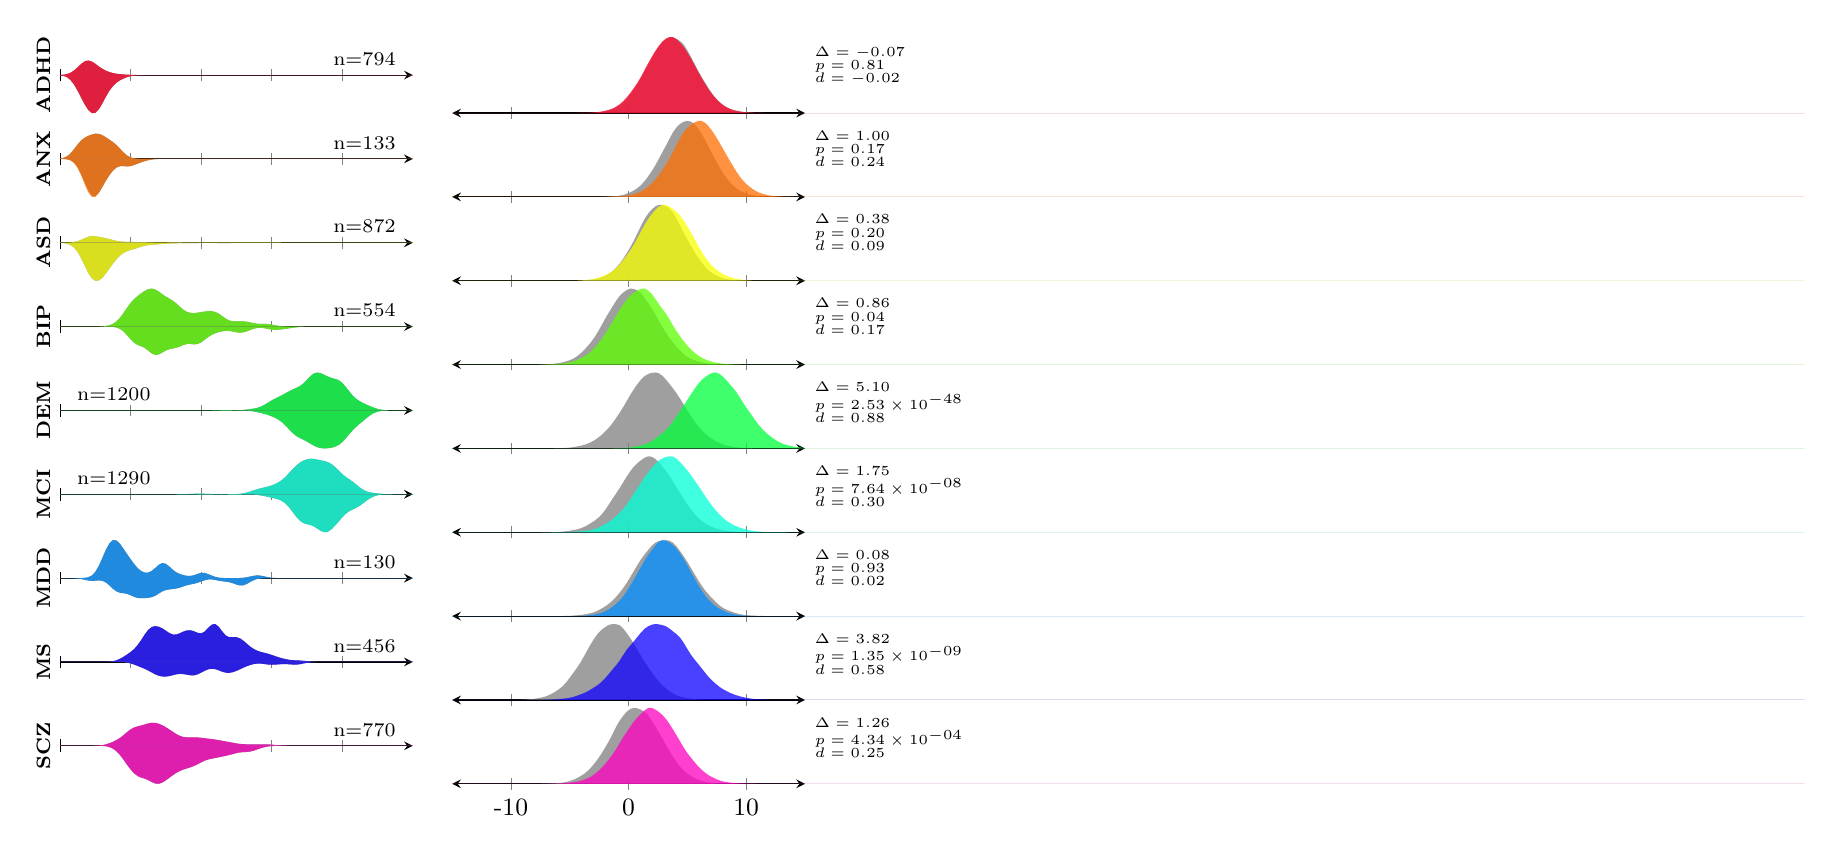
\begin{tikzpicture}
            \begin{groupplot}[
                group style={
					group name=my plots,
                    group size=2 by 10,vertical sep=0.1cm,
                    horizontal sep=0.5cm
                },
                height=0.21\textwidth,
                width=0.5\textwidth,
            ]
                \nextgroupplot[
                    xmin=0,
                    xmax=100,
                    ymax=1,
                    ymin=-1,
                    ytick=\empty,
                    axis x line=middle,
                    axis y line=none,
                    xtick={0,20,40,60,80},
                    xticklabels={,,},
                    x axis line style={|-stealth},
                ]
                \addplot [
                    draw=none,
                    line width=0pt,
                    name path=zero,
                ] coordinates {(0,0) (100,0)};
                \addplot [
                    draw=none,
                    line width=0pt,
                    name path=F-HC,
                ] coordinates {
                    (0, 0.0033541139760089413)
                    (1, 0.009542710951373334)
                    (2, 0.026638639702573137)
                    (3, 0.06225635133778601)
                    (4, 0.1223768433957306)
                    (5, 0.20458466423390595)
                    (6, 0.29295534922585925)
                    (7, 0.36081713703044793)
                    (8, 0.38432145659124356)
                    (9, 0.3582026574879411)
                    (10, 0.2984240261603108)
                    (11, 0.22887076162513767)
                    (12, 0.16639923507989107)
                    (13, 0.11684878661079422)
                    (14, 0.07983356868385313)
                    (15, 0.053561581273473546)
                    (16, 0.036026629827481844)
                    (17, 0.024682787870863795)
                    (18, 0.016840084119417422)
                    (19, 0.010752773976533406)
                    (20, 0.0060124321726787704)
                    (21, 0.002806523300465741)
                    (22, 0.001063031357289528)
                    (23, 0.000321925793893992)
                    (24, 7.682562687224758e-05)
                    (25, 1.4577346147426665e-05)
                    (26, 1.9382657545933396e-06)
                    (27, 0.0)
                    (28, 0.0)
                    (29, 0.0)
                    (30, 0.0)
                    (31, 0.0)
                    (32, 0.0)
                    (33, 0.0)
                    (34, 0.0)
                    (35, 0.0)
                    (36, 0.0)
                    (37, 0.0)
                    (38, 0.0)
                    (39, 0.0)
                    (40, 0.0)
                    (41, 0.0)
                    (42, 0.0)
                    (43, 0.0)
                    (44, 0.0)
                    (45, 0.0)
                    (46, 0.0)
                    (47, 0.0)
                    (48, 0.0)
                    (49, 0.0)
                    (50, 0.0)
                    (51, 0.0)
                    (52, 0.0)
                    (53, 0.0)
                    (54, 0.0)
                    (55, 0.0)
                    (56, 0.0)
                    (57, 0.0)
                    (58, 0.0)
                    (59, 0.0)
                    (60, 0.0)
                    (61, 0.0)
                    (62, 0.0)
                    (63, 0.0)
                    (64, 0.0)
                    (65, 0.0)
                    (66, 0.0)
                    (67, 0.0)
                    (68, 0.0)
                    (69, 0.0)
                    (70, 0.0)
                    (71, 0.0)
                    (72, 0.0)
                    (73, 0.0)
                    (74, 0.0)
                    (75, 0.0)
                    (76, 0.0)
                    (77, 0.0)
                    (78, 0.0)
                    (79, 0.0)
                    (80, 0.0)
                    (81, 0.0)
                    (82, 0.0)
                    (83, 0.0)
                    (84, 0.0)
                    (85, 0.0)
                    (86, 0.0)
                    (87, 0.0)
                    (88, 0.0)
                    (89, 0.0)
                    (90, 0.0)
                    (91, 0.0)
                    (92, 0.0)
                    (93, 0.0)
                    (94, 0.0)
                    (95, 0.0)
                    (96, 0.0)
                    (97, 0.0)
                    (98, 0.0)
                    (99, 0.0)
                };
                \addplot[
                    HC,
                    opacity=1,
                ] fill between [
                    of=zero and F-HC
                ];
                \addplot [
                    draw=none,
                    line width=0pt,
                    name path=F-ADHD,
                ] coordinates {
                    (0, 0.0033541139760089413)
                    (1, 0.009542710951373334)
                    (2, 0.026638639702573137)
                    (3, 0.06225635133778601)
                    (4, 0.1223768433957306)
                    (5, 0.20458466423390595)
                    (6, 0.29295534922585925)
                    (7, 0.36081713703044793)
                    (8, 0.38432145659124356)
                    (9, 0.3582026574879411)
                    (10, 0.2984240261603108)
                    (11, 0.22887076162513767)
                    (12, 0.16639923507989107)
                    (13, 0.11684878661079422)
                    (14, 0.07983356868385313)
                    (15, 0.053561581273473546)
                    (16, 0.036026629827481844)
                    (17, 0.024682787870863795)
                    (18, 0.016840084119417422)
                    (19, 0.010752773976533406)
                    (20, 0.0060124321726787704)
                    (21, 0.002806523300465741)
                    (22, 0.001063031357289528)
                    (23, 0.000321925793893992)
                    (24, 7.682562687224758e-05)
                    (25, 1.4577346147426665e-05)
                    (26, 1.9382657545933396e-06)
                    (27, 0.0)
                    (28, 0.0)
                    (29, 0.0)
                    (30, 0.0)
                    (31, 0.0)
                    (32, 0.0)
                    (33, 0.0)
                    (34, 0.0)
                    (35, 0.0)
                    (36, 0.0)
                    (37, 0.0)
                    (38, 0.0)
                    (39, 0.0)
                    (40, 0.0)
                    (41, 0.0)
                    (42, 0.0)
                    (43, 0.0)
                    (44, 0.0)
                    (45, 0.0)
                    (46, 0.0)
                    (47, 0.0)
                    (48, 0.0)
                    (49, 0.0)
                    (50, 0.0)
                    (51, 0.0)
                    (52, 0.0)
                    (53, 0.0)
                    (54, 0.0)
                    (55, 0.0)
                    (56, 0.0)
                    (57, 0.0)
                    (58, 0.0)
                    (59, 0.0)
                    (60, 0.0)
                    (61, 0.0)
                    (62, 0.0)
                    (63, 0.0)
                    (64, 0.0)
                    (65, 0.0)
                    (66, 0.0)
                    (67, 0.0)
                    (68, 0.0)
                    (69, 0.0)
                    (70, 0.0)
                    (71, 0.0)
                    (72, 0.0)
                    (73, 0.0)
                    (74, 0.0)
                    (75, 0.0)
                    (76, 0.0)
                    (77, 0.0)
                    (78, 0.0)
                    (79, 0.0)
                    (80, 0.0)
                    (81, 0.0)
                    (82, 0.0)
                    (83, 0.0)
                    (84, 0.0)
                    (85, 0.0)
                    (86, 0.0)
                    (87, 0.0)
                    (88, 0.0)
                    (89, 0.0)
                    (90, 0.0)
                    (91, 0.0)
                    (92, 0.0)
                    (93, 0.0)
                    (94, 0.0)
                    (95, 0.0)
                    (96, 0.0)
                    (97, 0.0)
                    (98, 0.0)
                    (99, 0.0)
                };
                \addplot[
                    ADHD,
                    opacity=0.75,
                ] fill between [
                    of=zero and F-ADHD
                ];
                \addplot [
                    draw=none,
                    line width=0pt,
                    name path=M-HC,
                ] coordinates {
                    (0, -0.007163570434233723)
                    (1, -0.02054246336366265)
                    (2, -0.05707201782883754)
                    (3, -0.13116685929022828)
                    (4, -0.25144620461565376)
                    (5, -0.4119122679537567)
                    (6, -0.5932379854799491)
                    (7, -0.7705632926880278)
                    (8, -0.9163074364723206)
                    (9, -1.0)
                    (10, -0.997275646643908)
                    (11, -0.9056019134115912)
                    (12, -0.750404821007498)
                    (13, -0.5737761878923834)
                    (14, -0.41403398067171043)
                    (15, -0.2905822153308525)
                    (16, -0.20261554134590265)
                    (17, -0.13928257720802226)
                    (18, -0.09125376614336109)
                    (19, -0.054957013730298494)
                    (20, -0.0296854615441586)
                    (21, -0.01416027499395819)
                    (22, -0.005860157610643177)
                    (23, -0.002057889414725279)
                    (24, -0.0005990660402045287)
                    (25, -0.00014000268748638853)
                    (26, -2.527816078566665e-05)
                    (27, -3.876531509186679e-06)
                    (28, -0.0)
                    (29, -0.0)
                    (30, -0.0)
                    (31, -0.0)
                    (32, -0.0)
                    (33, -0.0)
                    (34, -0.0)
                    (35, -0.0)
                    (36, -0.0)
                    (37, -0.0)
                    (38, -0.0)
                    (39, -0.0)
                    (40, -0.0)
                    (41, -0.0)
                    (42, -0.0)
                    (43, -0.0)
                    (44, -0.0)
                    (45, -0.0)
                    (46, -0.0)
                    (47, -0.0)
                    (48, -0.0)
                    (49, -0.0)
                    (50, -0.0)
                    (51, -0.0)
                    (52, -0.0)
                    (53, -0.0)
                    (54, -0.0)
                    (55, -0.0)
                    (56, -0.0)
                    (57, -0.0)
                    (58, -0.0)
                    (59, -0.0)
                    (60, -0.0)
                    (61, -0.0)
                    (62, -0.0)
                    (63, -0.0)
                    (64, -0.0)
                    (65, -0.0)
                    (66, -0.0)
                    (67, -0.0)
                    (68, -0.0)
                    (69, -0.0)
                    (70, -0.0)
                    (71, -0.0)
                    (72, -0.0)
                    (73, -0.0)
                    (74, -0.0)
                    (75, -0.0)
                    (76, -0.0)
                    (77, -0.0)
                    (78, -0.0)
                    (79, -0.0)
                    (80, -0.0)
                    (81, -0.0)
                    (82, -0.0)
                    (83, -0.0)
                    (84, -0.0)
                    (85, -0.0)
                    (86, -0.0)
                    (87, -0.0)
                    (88, -0.0)
                    (89, -0.0)
                    (90, -0.0)
                    (91, -0.0)
                    (92, -0.0)
                    (93, -0.0)
                    (94, -0.0)
                    (95, -0.0)
                    (96, -0.0)
                    (97, -0.0)
                    (98, -0.0)
                    (99, -0.0)
                };
                \addplot[
                    HC,
                    opacity=1,
                ] fill between [
                    of=zero and M-HC
                ];
                \addplot [
                    draw=none,
                    line width=0pt,
                    name path=M-ADHD,
                ] coordinates {
                    (0, -0.007163570434233723)
                    (1, -0.02054246336366265)
                    (2, -0.05707201782883754)
                    (3, -0.13116685929022828)
                    (4, -0.25144620461565376)
                    (5, -0.4119122679537567)
                    (6, -0.5932379854799491)
                    (7, -0.7705632926880278)
                    (8, -0.9163074364723206)
                    (9, -1.0)
                    (10, -0.997275646643908)
                    (11, -0.9056019134115912)
                    (12, -0.750404821007498)
                    (13, -0.5737761878923834)
                    (14, -0.41403398067171043)
                    (15, -0.2905822153308525)
                    (16, -0.20261554134590265)
                    (17, -0.13928257720802226)
                    (18, -0.09125376614336109)
                    (19, -0.054957013730298494)
                    (20, -0.0296854615441586)
                    (21, -0.01416027499395819)
                    (22, -0.005860157610643177)
                    (23, -0.002057889414725279)
                    (24, -0.0005990660402045287)
                    (25, -0.00014000268748638853)
                    (26, -2.527816078566665e-05)
                    (27, -3.876531509186679e-06)
                    (28, -0.0)
                    (29, -0.0)
                    (30, -0.0)
                    (31, -0.0)
                    (32, -0.0)
                    (33, -0.0)
                    (34, -0.0)
                    (35, -0.0)
                    (36, -0.0)
                    (37, -0.0)
                    (38, -0.0)
                    (39, -0.0)
                    (40, -0.0)
                    (41, -0.0)
                    (42, -0.0)
                    (43, -0.0)
                    (44, -0.0)
                    (45, -0.0)
                    (46, -0.0)
                    (47, -0.0)
                    (48, -0.0)
                    (49, -0.0)
                    (50, -0.0)
                    (51, -0.0)
                    (52, -0.0)
                    (53, -0.0)
                    (54, -0.0)
                    (55, -0.0)
                    (56, -0.0)
                    (57, -0.0)
                    (58, -0.0)
                    (59, -0.0)
                    (60, -0.0)
                    (61, -0.0)
                    (62, -0.0)
                    (63, -0.0)
                    (64, -0.0)
                    (65, -0.0)
                    (66, -0.0)
                    (67, -0.0)
                    (68, -0.0)
                    (69, -0.0)
                    (70, -0.0)
                    (71, -0.0)
                    (72, -0.0)
                    (73, -0.0)
                    (74, -0.0)
                    (75, -0.0)
                    (76, -0.0)
                    (77, -0.0)
                    (78, -0.0)
                    (79, -0.0)
                    (80, -0.0)
                    (81, -0.0)
                    (82, -0.0)
                    (83, -0.0)
                    (84, -0.0)
                    (85, -0.0)
                    (86, -0.0)
                    (87, -0.0)
                    (88, -0.0)
                    (89, -0.0)
                    (90, -0.0)
                    (91, -0.0)
                    (92, -0.0)
                    (93, -0.0)
                    (94, -0.0)
                    (95, -0.0)
                    (96, -0.0)
                    (97, -0.0)
                    (98, -0.0)
                    (99, -0.0)
                };
                \addplot[
                    ADHD,
                    opacity=0.75,
                ] fill between [
                    of=zero and M-ADHD
                ];
                \node[
                    anchor=south east
                ] at (axis cs: 100, 0) {
                    \scriptsize{
                    n=794
                    }
                };
                \nextgroupplot[
                    xmin=-15,
                    xmax=15,
                    ymax=1,
                    ymin=0,
                    ytick=\empty,
                    axis x line=bottom,
                    xtick={-10,0,10},
                    xticklabels=\empty,
                    axis y line=none,
                    x axis line style={stealth-stealth},
					clip=false
                ]
                \addplot [
                    draw=none,
                    line width=0pt,
                    name path=zero,
                ] coordinates {(0,0) (100,0)};
                \addplot [
                    draw=none,
                    line width=0pt,
                    name path=HC,
                ] coordinates {
                    (-15.0, 0.0)
                    (-14.696969696969697, 0.0)
                    (-14.393939393939394, 0.0)
                    (-14.09090909090909, 0.0)
                    (-13.787878787878787, 0.0)
                    (-13.484848484848484, 0.0)
                    (-13.181818181818182, 0.0)
                    (-12.878787878787879, 0.0)
                    (-12.575757575757576, 0.0)
                    (-12.272727272727273, 0.0)
                    (-11.969696969696969, 0.0)
                    (-11.666666666666666, 0.0)
                    (-11.363636363636363, 0.0)
                    (-11.06060606060606, 0.0)
                    (-10.757575757575758, 0.0)
                    (-10.454545454545453, 0.0)
                    (-10.151515151515152, 0.0)
                    (-9.848484848484848, 0.0)
                    (-9.545454545454545, 0.0)
                    (-9.242424242424242, 0.0)
                    (-8.93939393939394, 0.0)
                    (-8.636363636363637, 0.0)
                    (-8.333333333333332, 0.0)
                    (-8.030303030303031, 0.0)
                    (-7.727272727272727, 0.0)
                    (-7.424242424242424, 0.0)
                    (-7.121212121212121, 0.0)
                    (-6.818181818181818, 0.0)
                    (-6.515151515151516, 0.0)
                    (-6.212121212121211, 0.0)
                    (-5.909090909090908, 0.0)
                    (-5.6060606060606055, 0.0)
                    (-5.303030303030303, 0.00017319016279875303)
                    (-5.0, 0.00034638032559750607)
                    (-4.696969696969697, 0.0005195704883962591)
                    (-4.3939393939393945, 0.0005195704883962591)
                    (-4.09090909090909, 0.0006927606511950121)
                    (-3.787878787878787, 0.0013855213023900243)
                    (-3.4848484848484844, 0.0020782819535850364)
                    (-3.1818181818181817, 0.0032906130931763078)
                    (-2.878787878787879, 0.005542085209560097)
                    (-2.575757575757576, 0.009698649116730169)
                    (-2.2727272727272716, 0.016453065465881538)
                    (-1.9696969696969688, 0.024939383443020435)
                    (-1.666666666666666, 0.03654312435053689)
                    (-1.3636363636363633, 0.05351576030481469)
                    (-1.0606060606060606, 0.07603048146865259)
                    (-0.7575757575757578, 0.10408728784205057)
                    (-0.45454545454545325, 0.14028403186698996)
                    (-0.1515151515151505, 0.1891236577762383)
                    (0.15151515151515227, 0.24627641149982682)
                    (0.45454545454545503, 0.3115691028749567)
                    (0.7575757575757578, 0.3860408728784205)
                    (1.0606060606060623, 0.4683062002078282)
                    (1.3636363636363633, 0.5549012816072048)
                    (1.6666666666666679, 0.638205749913405)
                    (1.9696969696969688, 0.7209906477312089)
                    (2.2727272727272734, 0.803602355386214)
                    (2.575757575757578, 0.8782473155524766)
                    (2.878787878787879, 0.9348804987876689)
                    (3.1818181818181834, 0.9755801870453759)
                    (3.4848484848484844, 1.0)
                    (3.787878787878789, 0.99722895739522)
                    (4.09090909090909, 0.9748874263941808)
                    (4.3939393939393945, 0.9457914790439903)
                    (4.696969696969699, 0.8978178039487357)
                    (5.0, 0.824731555247662)
                    (5.3030303030303045, 0.7388292344994805)
                    (5.6060606060606055, 0.6485971596813301)
                    (5.90909090909091, 0.557499134049186)
                    (6.212121212121211, 0.4741946657429858)
                    (6.515151515151516, 0.3981641842743332)
                    (6.81818181818182, 0.3238656044336682)
                    (7.121212121212121, 0.2530308278489782)
                    (7.424242424242426, 0.19189470038101836)
                    (7.727272727272727, 0.14478697609975755)
                    (8.030303030303031, 0.10720471077242813)
                    (8.333333333333336, 0.07724281260824385)
                    (8.636363636363637, 0.05576723242119848)
                    (8.939393939393941, 0.0398337374437132)
                    (9.242424242424242, 0.02805680637339799)
                    (9.545454545454547, 0.019397298233460338)
                    (9.848484848484848, 0.012642881884308971)
                    (10.151515151515152, 0.007793557325943886)
                    (10.454545454545457, 0.004676134395566332)
                    (10.757575757575758, 0.0027710426047800486)
                    (11.060606060606062, 0.0015587114651887772)
                    (11.363636363636363, 0.0006927606511950121)
                    (11.666666666666668, 0.00034638032559750607)
                    (11.969696969696969, 0.00017319016279875303)
                    (12.272727272727273, 0.00017319016279875303)
                    (12.575757575757578, 0.0)
                    (12.878787878787879, 0.0)
                    (13.181818181818183, 0.0)
                    (13.484848484848484, 0.0)
                    (13.787878787878789, 0.0)
                    (14.090909090909093, 0.0)
                    (14.393939393939394, 0.0)
                    (14.696969696969699, 0.0)
                    (15.0, 0.0)
                };
                \addplot[
                    HC,
                    opacity=0.75,
                ] fill between [
                    of=zero and HC
                ];
                \addplot [
                    draw=none,
                    line width=0pt,
                    name path=ADHD,
                ] coordinates {
                    (-15.0, 0.0)
                    (-14.696969696969697, 0.0)
                    (-14.393939393939394, 0.0)
                    (-14.09090909090909, 0.0)
                    (-13.787878787878787, 0.0)
                    (-13.484848484848484, 0.0)
                    (-13.181818181818182, 0.0)
                    (-12.878787878787879, 0.0)
                    (-12.575757575757576, 0.0)
                    (-12.272727272727273, 0.0)
                    (-11.969696969696969, 0.0)
                    (-11.666666666666666, 0.0)
                    (-11.363636363636363, 0.0)
                    (-11.06060606060606, 0.0)
                    (-10.757575757575758, 0.0)
                    (-10.454545454545453, 0.0)
                    (-10.151515151515152, 0.0)
                    (-9.848484848484848, 0.0)
                    (-9.545454545454545, 0.0)
                    (-9.242424242424242, 0.0)
                    (-8.93939393939394, 0.0)
                    (-8.636363636363637, 0.0)
                    (-8.333333333333332, 0.0)
                    (-8.030303030303031, 0.0)
                    (-7.727272727272727, 0.0)
                    (-7.424242424242424, 0.0)
                    (-7.121212121212121, 0.0)
                    (-6.818181818181818, 0.0)
                    (-6.515151515151516, 0.0)
                    (-6.212121212121211, 0.0)
                    (-5.909090909090908, 0.0)
                    (-5.6060606060606055, 0.0)
                    (-5.303030303030303, 0.0)
                    (-5.0, 0.00017358097552508245)
                    (-4.696969696969697, 0.0005207429265752473)
                    (-4.3939393939393945, 0.0006943239021003298)
                    (-4.09090909090909, 0.0010414858531504947)
                    (-3.787878787878787, 0.0020829717063009894)
                    (-3.4848484848484844, 0.0032980385349765666)
                    (-3.1818181818181817, 0.005033848290227391)
                    (-2.878787878787879, 0.008331886825203957)
                    (-2.575757575757576, 0.013712897066481513)
                    (-2.2727272727272716, 0.021176879014060058)
                    (-1.9696969696969688, 0.030723832667939596)
                    (-1.666666666666666, 0.04304808193022045)
                    (-1.3636363636363633, 0.05988543655615344)
                    (-1.0606060606060606, 0.08383961117861483)
                    (-0.7575757575757578, 0.11629925360180524)
                    (-0.45454545454545325, 0.15761152577677487)
                    (-0.1515151515151505, 0.20847075160562403)
                    (0.15151515151515227, 0.2678354452352022)
                    (0.45454545454545503, 0.3318868252039576)
                    (0.7575757575757578, 0.40010414858531507)
                    (1.0606060606060623, 0.4796042353758028)
                    (1.3636363636363633, 0.5681305328935948)
                    (1.6666666666666679, 0.656830411386912)
                    (1.9696969696969688, 0.7404964415900017)
                    (2.2727272727272734, 0.8170456517965631)
                    (2.575757575757578, 0.8845686512758202)
                    (2.878787878787879, 0.9420239541746225)
                    (3.1818181818181834, 0.9814268356188162)
                    (3.4848484848484844, 1.0)
                    (3.787878787878789, 0.9980906092692241)
                    (4.09090909090909, 0.9703176531852109)
                    (4.3939393939393945, 0.9244922756465891)
                    (4.696969696969699, 0.8680784586009374)
                    (5.0, 0.7969102586356536)
                    (5.3030303030303045, 0.7175837528206909)
                    (5.6060606060606055, 0.6325290748134005)
                    (5.90909090909091, 0.5448706821732339)
                    (6.212121212121211, 0.4612046519701441)
                    (6.515151515151516, 0.38031591737545567)
                    (6.81818181818182, 0.3065440027772956)
                    (7.121212121212121, 0.24474917549036626)
                    (7.424242424242426, 0.19250130185731643)
                    (7.727272727272727, 0.14424579066134352)
                    (8.030303030303031, 0.10449574726609964)
                    (8.333333333333336, 0.07568130532893595)
                    (8.636363636363637, 0.05328935948620031)
                    (8.939393939393941, 0.03679916681131748)
                    (9.242424242424242, 0.02603714632876237)
                    (9.545454545454547, 0.018226002430133656)
                    (9.848484848484848, 0.01197708731123069)
                    (10.151515151515152, 0.007637562923103628)
                    (10.454545454545457, 0.004686686339177226)
                    (10.757575757575758, 0.0027772956084013193)
                    (11.060606060606062, 0.0013886478042006596)
                    (11.363636363636363, 0.0006943239021003298)
                    (11.666666666666668, 0.0003471619510501649)
                    (11.969696969696969, 0.00017358097552508245)
                    (12.272727272727273, 0.00017358097552508245)
                    (12.575757575757578, 0.0)
                    (12.878787878787879, 0.0)
                    (13.181818181818183, 0.0)
                    (13.484848484848484, 0.0)
                    (13.787878787878789, 0.0)
                    (14.090909090909093, 0.0)
                    (14.393939393939394, 0.0)
                    (14.696969696969699, 0.0)
                    (15.0, 0.0)
                };
                \addplot[
                    ADHD,
                    opacity=0.75,
                ] fill between [
                    of=zero and ADHD
                ];
                \node[
                    anchor=north west,
                    align=left,
                    font=\tiny\linespread{0.8}\selectfont
                ] at (axis cs: 15, 1.0) {
                    $\Delta=-0.07$\\
                    $p=0.81$\\
                    $d=-0.02$\\
                };

                \nextgroupplot[
                    xmin=0,
                    xmax=100,
                    ymax=1,
                    ymin=-1,
                    ytick=\empty,
                    axis x line=middle,
                    axis y line=none,
                    xtick={0,20,40,60,80},
                    xticklabels={,,},
                    x axis line style={|-stealth},
                ]
                \addplot [
                    draw=none,
                    line width=0pt,
                    name path=zero,
                ] coordinates {(0,0) (100,0)};
                \addplot [
                    draw=none,
                    line width=0pt,
                    name path=F-HC,
                ] coordinates {
                    (0, 0.009783668179707621)
                    (1, 0.026411059679050938)
                    (2, 0.06881676719760994)
                    (3, 0.14679150172521743)
                    (4, 0.25744111117145974)
                    (5, 0.37942728222108857)
                    (6, 0.48467449339158303)
                    (7, 0.5583244465811767)
                    (8, 0.6060688030360811)
                    (9, 0.6407306634319166)
                    (10, 0.6631927666009042)
                    (11, 0.6606092144512344)
                    (12, 0.6254355627315347)
                    (13, 0.5687463618384394)
                    (14, 0.5072019158298345)
                    (15, 0.44287425805124836)
                    (16, 0.36507619139272307)
                    (17, 0.27011968234160566)
                    (18, 0.17184424993453615)
                    (19, 0.0912525450995273)
                    (20, 0.03966788519895719)
                    (21, 0.013951266639772843)
                    (22, 0.003936441793869958)
                    (23, 0.000880998980588512)
                    (24, 0.00015626226963170463)
                    (25, 1.6412691771239807e-05)
                    (26, 0.0)
                    (27, 0.0)
                    (28, 0.0)
                    (29, 0.0)
                    (30, 0.0)
                    (31, 0.0)
                    (32, 0.0)
                    (33, 0.0)
                    (34, 0.0)
                    (35, 0.0)
                    (36, 0.0)
                    (37, 0.0)
                    (38, 0.0)
                    (39, 0.0)
                    (40, 0.0)
                    (41, 0.0)
                    (42, 0.0)
                    (43, 0.0)
                    (44, 0.0)
                    (45, 0.0)
                    (46, 0.0)
                    (47, 0.0)
                    (48, 0.0)
                    (49, 0.0)
                    (50, 0.0)
                    (51, 0.0)
                    (52, 0.0)
                    (53, 0.0)
                    (54, 0.0)
                    (55, 0.0)
                    (56, 0.0)
                    (57, 0.0)
                    (58, 0.0)
                    (59, 0.0)
                    (60, 0.0)
                    (61, 0.0)
                    (62, 0.0)
                    (63, 0.0)
                    (64, 0.0)
                    (65, 0.0)
                    (66, 0.0)
                    (67, 0.0)
                    (68, 0.0)
                    (69, 0.0)
                    (70, 0.0)
                    (71, 0.0)
                    (72, 0.0)
                    (73, 0.0)
                    (74, 0.0)
                    (75, 0.0)
                    (76, 0.0)
                    (77, 0.0)
                    (78, 0.0)
                    (79, 0.0)
                    (80, 0.0)
                    (81, 0.0)
                    (82, 0.0)
                    (83, 0.0)
                    (84, 0.0)
                    (85, 0.0)
                    (86, 0.0)
                    (87, 0.0)
                    (88, 0.0)
                    (89, 0.0)
                    (90, 0.0)
                    (91, 0.0)
                    (92, 0.0)
                    (93, 0.0)
                    (94, 0.0)
                    (95, 0.0)
                    (96, 0.0)
                    (97, 0.0)
                    (98, 0.0)
                    (99, 0.0)
                };
                \addplot[
                    HC,
                    opacity=1,
                ] fill between [
                    of=zero and F-HC
                ];
                \addplot [
                    draw=none,
                    line width=0pt,
                    name path=F-ANX,
                ] coordinates {
                    (0, 0.009783668179707621)
                    (1, 0.026411059679050938)
                    (2, 0.06881676719760994)
                    (3, 0.14679150172521743)
                    (4, 0.25744111117145974)
                    (5, 0.37942728222108857)
                    (6, 0.48467449339158303)
                    (7, 0.5583244465811767)
                    (8, 0.6060688030360811)
                    (9, 0.6407306634319166)
                    (10, 0.6631927666009042)
                    (11, 0.6606092144512344)
                    (12, 0.6254355627315347)
                    (13, 0.5687463618384394)
                    (14, 0.5072019158298345)
                    (15, 0.44287425805124836)
                    (16, 0.36507619139272307)
                    (17, 0.27011968234160566)
                    (18, 0.17184424993453615)
                    (19, 0.0912525450995273)
                    (20, 0.03966788519895719)
                    (21, 0.013951266639772843)
                    (22, 0.003936441793869958)
                    (23, 0.000880998980588512)
                    (24, 0.00015626226963170463)
                    (25, 1.6412691771239807e-05)
                    (26, 0.0)
                    (27, 0.0)
                    (28, 0.0)
                    (29, 0.0)
                    (30, 0.0)
                    (31, 0.0)
                    (32, 0.0)
                    (33, 0.0)
                    (34, 0.0)
                    (35, 0.0)
                    (36, 0.0)
                    (37, 0.0)
                    (38, 0.0)
                    (39, 0.0)
                    (40, 0.0)
                    (41, 0.0)
                    (42, 0.0)
                    (43, 0.0)
                    (44, 0.0)
                    (45, 0.0)
                    (46, 0.0)
                    (47, 0.0)
                    (48, 0.0)
                    (49, 0.0)
                    (50, 0.0)
                    (51, 0.0)
                    (52, 0.0)
                    (53, 0.0)
                    (54, 0.0)
                    (55, 0.0)
                    (56, 0.0)
                    (57, 0.0)
                    (58, 0.0)
                    (59, 0.0)
                    (60, 0.0)
                    (61, 0.0)
                    (62, 0.0)
                    (63, 0.0)
                    (64, 0.0)
                    (65, 0.0)
                    (66, 0.0)
                    (67, 0.0)
                    (68, 0.0)
                    (69, 0.0)
                    (70, 0.0)
                    (71, 0.0)
                    (72, 0.0)
                    (73, 0.0)
                    (74, 0.0)
                    (75, 0.0)
                    (76, 0.0)
                    (77, 0.0)
                    (78, 0.0)
                    (79, 0.0)
                    (80, 0.0)
                    (81, 0.0)
                    (82, 0.0)
                    (83, 0.0)
                    (84, 0.0)
                    (85, 0.0)
                    (86, 0.0)
                    (87, 0.0)
                    (88, 0.0)
                    (89, 0.0)
                    (90, 0.0)
                    (91, 0.0)
                    (92, 0.0)
                    (93, 0.0)
                    (94, 0.0)
                    (95, 0.0)
                    (96, 0.0)
                    (97, 0.0)
                    (98, 0.0)
                    (99, 0.0)
                };
                \addplot[
                    ANX,
                    opacity=0.75,
                ] fill between [
                    of=zero and F-ANX
                ];
                \addplot [
                    draw=none,
                    line width=0pt,
                    name path=M-HC,
                ] coordinates {
                    (0, -0.0005265729278993798)
                    (1, -0.002502992054487915)
                    (2, -0.010533226549173184)
                    (3, -0.03529707844429036)
                    (4, -0.09553096054580092)
                    (5, -0.21204458359711348)
                    (6, -0.3924669234569095)
                    (7, -0.6155782047148125)
                    (8, -0.8286427182478311)
                    (9, -0.9658813345545971)
                    (10, -0.9841162012208597)
                    (11, -0.8914524923917861)
                    (12, -0.7381557906262715)
                    (13, -0.5757135648140971)
                    (14, -0.4299164195045541)
                    (15, -0.31047553117039106)
                    (16, -0.22834907739576218)
                    (17, -0.1915498206823786)
                    (18, -0.19024701584613432)
                    (19, -0.19780066715981018)
                    (20, -0.19016052356693547)
                    (21, -0.16239356784101805)
                    (22, -0.1251713281000681)
                    (23, -0.08948054572027075)
                    (24, -0.05911249857922728)
                    (25, -0.03462465757127349)
                    (26, -0.017094263076956075)
                    (27, -0.006851813519646628)
                    (28, -0.002182463790190784)
                    (29, -0.0005435137058633164)
                    (30, -0.00010702419431798523)
                    (31, -1.6412691771239807e-05)
                    (32, -0.0)
                    (33, -0.0)
                    (34, -0.0)
                    (35, -0.0)
                    (36, -0.0)
                    (37, -0.0)
                    (38, -0.0)
                    (39, -0.0)
                    (40, -0.0)
                    (41, -0.0)
                    (42, -0.0)
                    (43, -0.0)
                    (44, -0.0)
                    (45, -0.0)
                    (46, -0.0)
                    (47, -0.0)
                    (48, -0.0)
                    (49, -0.0)
                    (50, -0.0)
                    (51, -0.0)
                    (52, -0.0)
                    (53, -0.0)
                    (54, -0.0)
                    (55, -0.0)
                    (56, -0.0)
                    (57, -0.0)
                    (58, -0.0)
                    (59, -0.0)
                    (60, -0.0)
                    (61, -0.0)
                    (62, -0.0)
                    (63, -0.0)
                    (64, -0.0)
                    (65, -0.0)
                    (66, -0.0)
                    (67, -0.0)
                    (68, -0.0)
                    (69, -0.0)
                    (70, -0.0)
                    (71, -0.0)
                    (72, -0.0)
                    (73, -0.0)
                    (74, -0.0)
                    (75, -0.0)
                    (76, -0.0)
                    (77, -0.0)
                    (78, -0.0)
                    (79, -0.0)
                    (80, -0.0)
                    (81, -0.0)
                    (82, -0.0)
                    (83, -0.0)
                    (84, -0.0)
                    (85, -0.0)
                    (86, -0.0)
                    (87, -0.0)
                    (88, -0.0)
                    (89, -0.0)
                    (90, -0.0)
                    (91, -0.0)
                    (92, -0.0)
                    (93, -0.0)
                    (94, -0.0)
                    (95, -0.0)
                    (96, -0.0)
                    (97, -0.0)
                    (98, -0.0)
                    (99, -0.0)
                };
                \addplot[
                    HC,
                    opacity=1,
                ] fill between [
                    of=zero and M-HC
                ];
                \addplot [
                    draw=none,
                    line width=0pt,
                    name path=M-ANX,
                ] coordinates {
                    (0, -0.0006500098139886048)
                    (1, -0.0030465057603512313)
                    (2, -0.01268286495582149)
                    (3, -0.041918430883529784)
                    (4, -0.11141475932494115)
                    (5, -0.24171942645490907)
                    (6, -0.4356435650451463)
                    (7, -0.6645037493391439)
                    (8, -0.8718193598360678)
                    (9, -0.9955561774123929)
                    (10, -1.0)
                    (11, -0.8980738448310256)
                    (12, -0.7403054290329197)
                    (13, -0.5762570785199603)
                    (14, -0.43002344369887197)
                    (15, -0.31049194386216233)
                    (16, -0.22834907739576218)
                    (17, -0.1915498206823786)
                    (18, -0.19024701584613432)
                    (19, -0.19780066715981018)
                    (20, -0.19016052356693547)
                    (21, -0.16239356784101805)
                    (22, -0.1251713281000681)
                    (23, -0.08948054572027075)
                    (24, -0.05911249857922728)
                    (25, -0.03462465757127349)
                    (26, -0.017094263076956075)
                    (27, -0.006851813519646628)
                    (28, -0.002182463790190784)
                    (29, -0.0005435137058633164)
                    (30, -0.00010702419431798523)
                    (31, -1.6412691771239807e-05)
                    (32, -0.0)
                    (33, -0.0)
                    (34, -0.0)
                    (35, -0.0)
                    (36, -0.0)
                    (37, -0.0)
                    (38, -0.0)
                    (39, -0.0)
                    (40, -0.0)
                    (41, -0.0)
                    (42, -0.0)
                    (43, -0.0)
                    (44, -0.0)
                    (45, -0.0)
                    (46, -0.0)
                    (47, -0.0)
                    (48, -0.0)
                    (49, -0.0)
                    (50, -0.0)
                    (51, -0.0)
                    (52, -0.0)
                    (53, -0.0)
                    (54, -0.0)
                    (55, -0.0)
                    (56, -0.0)
                    (57, -0.0)
                    (58, -0.0)
                    (59, -0.0)
                    (60, -0.0)
                    (61, -0.0)
                    (62, -0.0)
                    (63, -0.0)
                    (64, -0.0)
                    (65, -0.0)
                    (66, -0.0)
                    (67, -0.0)
                    (68, -0.0)
                    (69, -0.0)
                    (70, -0.0)
                    (71, -0.0)
                    (72, -0.0)
                    (73, -0.0)
                    (74, -0.0)
                    (75, -0.0)
                    (76, -0.0)
                    (77, -0.0)
                    (78, -0.0)
                    (79, -0.0)
                    (80, -0.0)
                    (81, -0.0)
                    (82, -0.0)
                    (83, -0.0)
                    (84, -0.0)
                    (85, -0.0)
                    (86, -0.0)
                    (87, -0.0)
                    (88, -0.0)
                    (89, -0.0)
                    (90, -0.0)
                    (91, -0.0)
                    (92, -0.0)
                    (93, -0.0)
                    (94, -0.0)
                    (95, -0.0)
                    (96, -0.0)
                    (97, -0.0)
                    (98, -0.0)
                    (99, -0.0)
                };
                \addplot[
                    ANX,
                    opacity=0.75,
                ] fill between [
                    of=zero and M-ANX
                ];
                \node[
                    anchor=south east
                ] at (axis cs: 100, 0) {
                    \scriptsize{
                    n=133
                    }
                };
                \nextgroupplot[
                    xmin=-15,
                    xmax=15,
                    ymax=1,
                    ymin=0,
                    ytick=\empty,
                    axis x line=bottom,
                    xtick={-10,0,10},
                    xticklabels=\empty,
                    axis y line=none,
                    x axis line style={stealth-stealth},
					clip=false
                ]
                \addplot [
                    draw=none,
                    line width=0pt,
                    name path=zero,
                ] coordinates {(0,0) (100,0)};
                \addplot [
                    draw=none,
                    line width=0pt,
                    name path=HC,
                ] coordinates {
                    (-15.0, 0.0)
                    (-14.696969696969697, 0.0)
                    (-14.393939393939394, 0.0)
                    (-14.09090909090909, 0.0)
                    (-13.787878787878787, 0.0)
                    (-13.484848484848484, 0.0)
                    (-13.181818181818182, 0.0)
                    (-12.878787878787879, 0.0)
                    (-12.575757575757576, 0.0)
                    (-12.272727272727273, 0.0)
                    (-11.969696969696969, 0.0)
                    (-11.666666666666666, 0.0)
                    (-11.363636363636363, 0.0)
                    (-11.06060606060606, 0.0)
                    (-10.757575757575758, 0.0)
                    (-10.454545454545453, 0.0)
                    (-10.151515151515152, 0.0)
                    (-9.848484848484848, 0.0)
                    (-9.545454545454545, 0.0)
                    (-9.242424242424242, 0.0)
                    (-8.93939393939394, 0.0)
                    (-8.636363636363637, 0.0)
                    (-8.333333333333332, 0.0)
                    (-8.030303030303031, 0.0)
                    (-7.727272727272727, 0.0)
                    (-7.424242424242424, 0.0)
                    (-7.121212121212121, 0.0)
                    (-6.818181818181818, 0.0)
                    (-6.515151515151516, 0.0)
                    (-6.212121212121211, 0.0)
                    (-5.909090909090908, 0.0)
                    (-5.6060606060606055, 0.0)
                    (-5.303030303030303, 0.0)
                    (-5.0, 0.0)
                    (-4.696969696969697, 0.0)
                    (-4.3939393939393945, 0.0)
                    (-4.09090909090909, 0.0)
                    (-3.787878787878787, 0.0)
                    (-3.4848484848484844, 0.0)
                    (-3.1818181818181817, 0.00016775708773695687)
                    (-2.878787878787879, 0.0005032712632108706)
                    (-2.575757575757576, 0.0011742996141586982)
                    (-2.2727272727272716, 0.001677570877369569)
                    (-1.9696969696969688, 0.002851870491528267)
                    (-1.666666666666666, 0.004529441368897836)
                    (-1.3636363636363633, 0.007213554772689146)
                    (-1.0606060606060606, 0.010904210702902198)
                    (-0.7575757575757578, 0.016775708773695688)
                    (-0.45454545454545325, 0.02700889112565006)
                    (-0.1515151515151505, 0.042274786109713136)
                    (0.15151515151515227, 0.061566851199463174)
                    (0.45454545454545503, 0.08538835765811105)
                    (0.7575757575757578, 0.11625566180171112)
                    (1.0606060606060623, 0.15618184868310686)
                    (1.3636363636363633, 0.2081865458815635)
                    (1.6666666666666679, 0.2704244254319745)
                    (1.9696969696969688, 0.3392048314041268)
                    (2.2727272727272734, 0.4158698204999161)
                    (2.575757575757578, 0.5014259352457642)
                    (2.878787878787879, 0.5898339204831404)
                    (3.1818181818181834, 0.677067606106358)
                    (3.4848484848484844, 0.7678241905720516)
                    (3.787878787878789, 0.8528770340546888)
                    (4.09090909090909, 0.9186378124475759)
                    (4.3939393939393945, 0.9625901694346586)
                    (4.696969696969699, 0.9904378459989934)
                    (5.0, 1.0)
                    (5.3030303030303045, 0.9911088743499413)
                    (5.6060606060606055, 0.9594027847676564)
                    (5.90909090909091, 0.9025331320248281)
                    (6.212121212121211, 0.8309008555611475)
                    (6.515151515151516, 0.7478610971313538)
                    (6.81818181818182, 0.6550914276128167)
                    (7.121212121212121, 0.5624895151820164)
                    (7.424242424242426, 0.474584801207851)
                    (7.727272727272727, 0.3903707431638987)
                    (8.030303030303031, 0.3132024828048985)
                    (8.333333333333336, 0.24559637644690488)
                    (8.636363636363637, 0.18922999496728737)
                    (8.939393939393941, 0.14259352457641336)
                    (9.242424242424242, 0.10501593692333501)
                    (9.545454545454547, 0.07582620365710452)
                    (9.848484848484848, 0.05385002516356316)
                    (10.151515151515152, 0.03724207347760443)
                    (10.454545454545457, 0.02432477772185875)
                    (10.757575757575758, 0.01560140915953699)
                    (11.060606060606062, 0.0097299110887435)
                    (11.363636363636363, 0.0062070122462674045)
                    (11.666666666666668, 0.0038584130179500084)
                    (11.969696969696969, 0.0023485992283173965)
                    (12.272727272727273, 0.001342056701895655)
                    (12.575757575757578, 0.0006710283509478275)
                    (12.878787878787879, 0.00033551417547391375)
                    (13.181818181818183, 0.00016775708773695687)
                    (13.484848484848484, 0.00016775708773695687)
                    (13.787878787878789, 0.00016775708773695687)
                    (14.090909090909093, 0.0)
                    (14.393939393939394, 0.0)
                    (14.696969696969699, 0.0)
                    (15.0, 0.0)
                };
                \addplot[
                    HC,
                    opacity=0.75,
                ] fill between [
                    of=zero and HC
                ];
                \addplot [
                    draw=none,
                    line width=0pt,
                    name path=ANX,
                ] coordinates {
                    (-15.0, 0.0)
                    (-14.696969696969697, 0.0)
                    (-14.393939393939394, 0.0)
                    (-14.09090909090909, 0.0)
                    (-13.787878787878787, 0.0)
                    (-13.484848484848484, 0.0)
                    (-13.181818181818182, 0.0)
                    (-12.878787878787879, 0.0)
                    (-12.575757575757576, 0.0)
                    (-12.272727272727273, 0.0)
                    (-11.969696969696969, 0.0)
                    (-11.666666666666666, 0.0)
                    (-11.363636363636363, 0.0)
                    (-11.06060606060606, 0.0)
                    (-10.757575757575758, 0.0)
                    (-10.454545454545453, 0.0)
                    (-10.151515151515152, 0.0)
                    (-9.848484848484848, 0.0)
                    (-9.545454545454545, 0.0)
                    (-9.242424242424242, 0.0)
                    (-8.93939393939394, 0.0)
                    (-8.636363636363637, 0.0)
                    (-8.333333333333332, 0.0)
                    (-8.030303030303031, 0.0)
                    (-7.727272727272727, 0.0)
                    (-7.424242424242424, 0.0)
                    (-7.121212121212121, 0.0)
                    (-6.818181818181818, 0.0)
                    (-6.515151515151516, 0.0)
                    (-6.212121212121211, 0.0)
                    (-5.909090909090908, 0.0)
                    (-5.6060606060606055, 0.0)
                    (-5.303030303030303, 0.0)
                    (-5.0, 0.0)
                    (-4.696969696969697, 0.0)
                    (-4.3939393939393945, 0.0)
                    (-4.09090909090909, 0.0)
                    (-3.787878787878787, 0.0)
                    (-3.4848484848484844, 0.0)
                    (-3.1818181818181817, 0.0)
                    (-2.878787878787879, 0.00017809439002671417)
                    (-2.575757575757576, 0.00035618878005342833)
                    (-2.2727272727272716, 0.0007123775601068567)
                    (-1.9696969696969688, 0.0014247551202137133)
                    (-1.666666666666666, 0.0021371326803205698)
                    (-1.3636363636363633, 0.003027604630454141)
                    (-1.0606060606060606, 0.004096170970614425)
                    (-0.7575757575757578, 0.006411398040961709)
                    (-0.45454545454545325, 0.010507569011576135)
                    (-0.1515151515151505, 0.01674087266251113)
                    (0.15151515151515227, 0.024933214603739984)
                    (0.45454545454545503, 0.0365093499554764)
                    (0.7575757575757578, 0.05182546749777382)
                    (1.0606060606060623, 0.07248441674087266)
                    (1.3636363636363633, 0.10008904719501335)
                    (1.6666666666666679, 0.13535173642030277)
                    (1.9696969696969688, 0.17773820124666073)
                    (2.2727272727272734, 0.2276046304541407)
                    (2.575757575757578, 0.2869100623330365)
                    (2.878787878787879, 0.35565449688334816)
                    (3.1818181818181834, 0.42831700801424755)
                    (3.4848484848484844, 0.5081032947462155)
                    (3.787878787878789, 0.5982190560997328)
                    (4.09090909090909, 0.6899376669634907)
                    (4.3939393939393945, 0.776313446126447)
                    (4.696969696969699, 0.8507569011576135)
                    (5.0, 0.9075690115761353)
                    (5.3030303030303045, 0.9481745325022262)
                    (5.6060606060606055, 0.980053428317008)
                    (5.90909090909091, 1.0)
                    (6.212121212121211, 0.9998219056099733)
                    (6.515151515151516, 0.9745325022261799)
                    (6.81818181818182, 0.9268032056990205)
                    (7.121212121212121, 0.8644701691896706)
                    (7.424242424242426, 0.7921638468388246)
                    (7.727272727272727, 0.7141585040071238)
                    (8.030303030303031, 0.6322350845948352)
                    (8.333333333333336, 0.5499554764024933)
                    (8.636363636363637, 0.46821015138023153)
                    (8.939393939393941, 0.38913624220837045)
                    (9.242424242424242, 0.31522707034728403)
                    (9.545454545454547, 0.24826357969723953)
                    (9.848484848484848, 0.19376669634906502)
                    (10.151515151515152, 0.15066785396260018)
                    (10.454545454545457, 0.11415850400712378)
                    (10.757575757575758, 0.08210151380231523)
                    (11.060606060606062, 0.05841495992876224)
                    (11.363636363636363, 0.04203027604630454)
                    (11.666666666666668, 0.02902938557435441)
                    (11.969696969696969, 0.019056099732858416)
                    (12.272727272727273, 0.013000890471950133)
                    (12.575757575757578, 0.008726625111308993)
                    (12.878787878787879, 0.005520926090828139)
                    (13.181818181818183, 0.003561887800534283)
                    (13.484848484848484, 0.002493321460373998)
                    (13.787878787878789, 0.0017809439002671415)
                    (14.090909090909093, 0.001246660730186999)
                    (14.393939393939394, 0.0007123775601068567)
                    (14.696969696969699, 0.00035618878005342833)
                    (15.0, 0.00017809439002671417)
                };
                \addplot[
                    ANX,
                    opacity=0.75,
                ] fill between [
                    of=zero and ANX
                ];
                \node[
                    anchor=north west,
                    align=left,
                    font=\tiny\linespread{0.8}\selectfont
                ] at (axis cs: 15, 1.0) {
                    $\Delta=1.00$\\
                    $p=0.17$\\
                    $d=0.24$\\
                };

                \nextgroupplot[
                    xmin=0,
                    xmax=100,
                    ymax=1,
                    ymin=-1,
                    ytick=\empty,
                    axis x line=middle,
                    axis y line=none,
                    xtick={0,20,40,60,80},
                    xticklabels={,,},
                    x axis line style={|-stealth},
                ]
                \addplot [
                    draw=none,
                    line width=0pt,
                    name path=zero,
                ] coordinates {(0,0) (100,0)};
                \addplot [
                    draw=none,
                    line width=0pt,
                    name path=F-HC,
                ] coordinates {
                    (0, 0.00034767859694427697)
                    (1, 0.0010140490778018161)
                    (2, 0.0030270532538809684)
                    (3, 0.008104358611665788)
                    (4, 0.019528053407895287)
                    (5, 0.041665181137739385)
                    (6, 0.07655969470246099)
                    (7, 0.11878423875141733)
                    (8, 0.15513562721824065)
                    (9, 0.173160964648492)
                    (10, 0.17076541153772865)
                    (11, 0.15578682526029644)
                    (12, 0.13685086411313502)
                    (13, 0.11685551975633188)
                    (14, 0.09489465067793403)
                    (15, 0.07155302430644277)
                    (16, 0.050442597719612764)
                    (17, 0.03525113679126226)
                    (18, 0.026728742421048574)
                    (19, 0.02280380423100914)
                    (20, 0.020918440877968673)
                    (21, 0.019626908700041492)
                    (22, 0.018373525642288516)
                    (23, 0.01672806896646497)
                    (24, 0.014308967748466107)
                    (25, 0.011117048788060833)
                    (26, 0.0076465568787799)
                    (27, 0.00470923651766336)
                    (28, 0.0031230647335126053)
                    (29, 0.0033984221552800483)
                    (30, 0.005458983096871945)
                    (31, 0.008378366419552166)
                    (32, 0.010523739336541061)
                    (33, 0.010513397941907202)
                    (34, 0.008314462613952345)
                    (35, 0.0051995594257707)
                    (36, 0.002568489027360544)
                    (37, 0.0010010238779619457)
                    (38, 0.0003073665927803089)
                    (39, 7.424520023367994e-05)
                    (40, 1.4087720825123836e-05)
                    (41, 1.873163095631727e-06)
                    (42, 0.0)
                    (43, 0.0)
                    (44, 0.0)
                    (45, 0.0)
                    (46, 1.873163095631727e-06)
                    (47, 1.2214557729492109e-05)
                    (48, 6.203064250418782e-05)
                    (49, 0.0002453359502761211)
                    (50, 0.0007556879276858245)
                    (51, 0.0018128010996747194)
                    (52, 0.0033867583260959815)
                    (53, 0.004927704287856364)
                    (54, 0.005583820490955205)
                    (55, 0.004927704287856364)
                    (56, 0.0033867583260959815)
                    (57, 0.0018128010996747194)
                    (58, 0.0007556879276858245)
                    (59, 0.0002453359502761211)
                    (60, 6.203064250418782e-05)
                    (61, 1.2214557729492109e-05)
                    (62, 1.873163095631727e-06)
                    (63, 0.0)
                    (64, 0.0)
                    (65, 0.0)
                    (66, 0.0)
                    (67, 0.0)
                    (68, 0.0)
                    (69, 0.0)
                    (70, 0.0)
                    (71, 0.0)
                    (72, 0.0)
                    (73, 0.0)
                    (74, 0.0)
                    (75, 0.0)
                    (76, 0.0)
                    (77, 0.0)
                    (78, 0.0)
                    (79, 0.0)
                    (80, 0.0)
                    (81, 0.0)
                    (82, 0.0)
                    (83, 0.0)
                    (84, 0.0)
                    (85, 0.0)
                    (86, 0.0)
                    (87, 0.0)
                    (88, 0.0)
                    (89, 0.0)
                    (90, 0.0)
                    (91, 0.0)
                    (92, 0.0)
                    (93, 0.0)
                    (94, 0.0)
                    (95, 0.0)
                    (96, 0.0)
                    (97, 0.0)
                    (98, 0.0)
                    (99, 0.0)
                };
                \addplot[
                    HC,
                    opacity=1,
                ] fill between [
                    of=zero and F-HC
                ];
                \addplot [
                    draw=none,
                    line width=0pt,
                    name path=F-ASD,
                ] coordinates {
                    (0, 0.00034767859694427697)
                    (1, 0.0010140490778018161)
                    (2, 0.0030270532538809684)
                    (3, 0.008104358611665788)
                    (4, 0.019528053407895287)
                    (5, 0.041665181137739385)
                    (6, 0.07655969470246099)
                    (7, 0.11878423875141733)
                    (8, 0.15513562721824065)
                    (9, 0.173160964648492)
                    (10, 0.17076541153772865)
                    (11, 0.15578682526029644)
                    (12, 0.13685086411313502)
                    (13, 0.11685551975633188)
                    (14, 0.09489465067793403)
                    (15, 0.07155302430644277)
                    (16, 0.050442597719612764)
                    (17, 0.03525113679126226)
                    (18, 0.026728742421048574)
                    (19, 0.02280380423100914)
                    (20, 0.020918440877968673)
                    (21, 0.019626908700041492)
                    (22, 0.018373525642288516)
                    (23, 0.01672806896646497)
                    (24, 0.014308967748466107)
                    (25, 0.011117048788060833)
                    (26, 0.0076465568787799)
                    (27, 0.00470923651766336)
                    (28, 0.0031230647335126053)
                    (29, 0.0033984221552800483)
                    (30, 0.005458983096871945)
                    (31, 0.008378366419552166)
                    (32, 0.010523739336541061)
                    (33, 0.010513397941907202)
                    (34, 0.008314462613952345)
                    (35, 0.0051995594257707)
                    (36, 0.002568489027360544)
                    (37, 0.0010010238779619457)
                    (38, 0.0003073665927803089)
                    (39, 7.424520023367994e-05)
                    (40, 1.4087720825123836e-05)
                    (41, 1.873163095631727e-06)
                    (42, 0.0)
                    (43, 0.0)
                    (44, 0.0)
                    (45, 0.0)
                    (46, 1.873163095631727e-06)
                    (47, 1.2214557729492109e-05)
                    (48, 6.203064250418782e-05)
                    (49, 0.0002453359502761211)
                    (50, 0.0007556879276858245)
                    (51, 0.0018128010996747194)
                    (52, 0.0033867583260959815)
                    (53, 0.004927704287856364)
                    (54, 0.005583820490955205)
                    (55, 0.004927704287856364)
                    (56, 0.0033867583260959815)
                    (57, 0.0018128010996747194)
                    (58, 0.0007556879276858245)
                    (59, 0.0002453359502761211)
                    (60, 6.203064250418782e-05)
                    (61, 1.2214557729492109e-05)
                    (62, 1.873163095631727e-06)
                    (63, 0.0)
                    (64, 0.0)
                    (65, 0.0)
                    (66, 0.0)
                    (67, 0.0)
                    (68, 0.0)
                    (69, 0.0)
                    (70, 0.0)
                    (71, 0.0)
                    (72, 0.0)
                    (73, 0.0)
                    (74, 0.0)
                    (75, 0.0)
                    (76, 0.0)
                    (77, 0.0)
                    (78, 0.0)
                    (79, 0.0)
                    (80, 0.0)
                    (81, 0.0)
                    (82, 0.0)
                    (83, 0.0)
                    (84, 0.0)
                    (85, 0.0)
                    (86, 0.0)
                    (87, 0.0)
                    (88, 0.0)
                    (89, 0.0)
                    (90, 0.0)
                    (91, 0.0)
                    (92, 0.0)
                    (93, 0.0)
                    (94, 0.0)
                    (95, 0.0)
                    (96, 0.0)
                    (97, 0.0)
                    (98, 0.0)
                    (99, 0.0)
                };
                \addplot[
                    ASD,
                    opacity=0.75,
                ] fill between [
                    of=zero and F-ASD
                ];
                \addplot [
                    draw=none,
                    line width=0pt,
                    name path=M-HC,
                ] coordinates {
                    (0, -0.0028306148600403397)
                    (1, -0.008212473982564644)
                    (2, -0.023674962669969747)
                    (3, -0.05857590252123645)
                    (4, -0.12604558679676436)
                    (5, -0.23920407092816268)
                    (6, -0.4020006259971605)
                    (7, -0.5976889189536916)
                    (8, -0.7880460496304132)
                    (9, -0.9306899976046176)
                    (10, -1.0)
                    (11, -0.9929731940068834)
                    (12, -0.922543741731014)
                    (13, -0.8103759599931174)
                    (14, -0.6801876378605368)
                    (15, -0.5507663339397006)
                    (16, -0.43404306056555914)
                    (17, -0.338117670886144)
                    (18, -0.2677972946433147)
                    (19, -0.2214249410716361)
                    (20, -0.1903671582841238)
                    (21, -0.16375668736018073)
                    (22, -0.13489120983740666)
                    (23, -0.10455204561354271)
                    (24, -0.07865428413148312)
                    (25, -0.06164641022448252)
                    (26, -0.0521736800466134)
                    (27, -0.04543704501061482)
                    (28, -0.038395751836472855)
                    (29, -0.03130525776860923)
                    (30, -0.025316492819158123)
                    (31, -0.020613313704686068)
                    (32, -0.016807000907743862)
                    (33, -0.013821813658159241)
                    (34, -0.011926238681750207)
                    (35, -0.011195937723380093)
                    (36, -0.011102961067235706)
                    (37, -0.010689088029823495)
                    (38, -0.009242217045881924)
                    (39, -0.00686643983563509)
                    (40, -0.0044018699248830504)
                    (41, -0.002827912698461789)
                    (42, -0.0026925503123689195)
                    (43, -0.0038896447843777163)
                    (44, -0.005747296021142008)
                    (45, -0.007408836148359416)
                    (46, -0.008316335777047977)
                    (47, -0.008314462613952345)
                    (48, -0.007396621590629925)
                    (49, -0.005685265378637821)
                    (50, -0.0036443088341015944)
                    (51, -0.001936862384683095)
                    (52, -0.0010132384356914376)
                    (53, -0.0010028970410575775)
                    (54, -0.001874831742178907)
                    (55, -0.003398972883825474)
                    (56, -0.004929577450951996)
                    (57, -0.005583820490955205)
                    (58, -0.004927704287856364)
                    (59, -0.0033867583260959815)
                    (60, -0.0018128010996747194)
                    (61, -0.0007556879276858245)
                    (62, -0.0002453359502761211)
                    (63, -6.203064250418782e-05)
                    (64, -1.2214557729492109e-05)
                    (65, -1.873163095631727e-06)
                    (66, -0.0)
                    (67, -0.0)
                    (68, -0.0)
                    (69, -0.0)
                    (70, -0.0)
                    (71, -0.0)
                    (72, -0.0)
                    (73, -0.0)
                    (74, -0.0)
                    (75, -0.0)
                    (76, -0.0)
                    (77, -0.0)
                    (78, -0.0)
                    (79, -0.0)
                    (80, -0.0)
                    (81, -0.0)
                    (82, -0.0)
                    (83, -0.0)
                    (84, -0.0)
                    (85, -0.0)
                    (86, -0.0)
                    (87, -0.0)
                    (88, -0.0)
                    (89, -0.0)
                    (90, -0.0)
                    (91, -0.0)
                    (92, -0.0)
                    (93, -0.0)
                    (94, -0.0)
                    (95, -0.0)
                    (96, -0.0)
                    (97, -0.0)
                    (98, -0.0)
                    (99, -0.0)
                };
                \addplot[
                    HC,
                    opacity=1,
                ] fill between [
                    of=zero and M-HC
                ];
                \addplot [
                    draw=none,
                    line width=0pt,
                    name path=M-ASD,
                ] coordinates {
                    (0, -0.0028306148600403397)
                    (1, -0.008212473982564644)
                    (2, -0.023674962669969747)
                    (3, -0.05857590252123645)
                    (4, -0.12604558679676436)
                    (5, -0.23920407092816268)
                    (6, -0.4020006259971605)
                    (7, -0.5976889189536916)
                    (8, -0.7880460496304132)
                    (9, -0.9306899976046176)
                    (10, -1.0)
                    (11, -0.9929731940068834)
                    (12, -0.922543741731014)
                    (13, -0.8103759599931174)
                    (14, -0.6801876378605368)
                    (15, -0.5507663339397006)
                    (16, -0.43404306056555914)
                    (17, -0.338117670886144)
                    (18, -0.2677972946433147)
                    (19, -0.2214249410716361)
                    (20, -0.1903671582841238)
                    (21, -0.16375668736018073)
                    (22, -0.13489120983740666)
                    (23, -0.10455204561354271)
                    (24, -0.07865428413148312)
                    (25, -0.06164641022448252)
                    (26, -0.0521736800466134)
                    (27, -0.04543704501061482)
                    (28, -0.038395751836472855)
                    (29, -0.03130525776860923)
                    (30, -0.025316492819158123)
                    (31, -0.020613313704686068)
                    (32, -0.016807000907743862)
                    (33, -0.013821813658159241)
                    (34, -0.011926238681750207)
                    (35, -0.011195937723380093)
                    (36, -0.011102961067235706)
                    (37, -0.010689088029823495)
                    (38, -0.009242217045881924)
                    (39, -0.00686643983563509)
                    (40, -0.0044018699248830504)
                    (41, -0.002827912698461789)
                    (42, -0.0026925503123689195)
                    (43, -0.0038896447843777163)
                    (44, -0.005747296021142008)
                    (45, -0.007408836148359416)
                    (46, -0.008316335777047977)
                    (47, -0.008314462613952345)
                    (48, -0.007396621590629925)
                    (49, -0.005685265378637821)
                    (50, -0.0036443088341015944)
                    (51, -0.001936862384683095)
                    (52, -0.0010132384356914376)
                    (53, -0.0010028970410575775)
                    (54, -0.001874831742178907)
                    (55, -0.003398972883825474)
                    (56, -0.004929577450951996)
                    (57, -0.005583820490955205)
                    (58, -0.004927704287856364)
                    (59, -0.0033867583260959815)
                    (60, -0.0018128010996747194)
                    (61, -0.0007556879276858245)
                    (62, -0.0002453359502761211)
                    (63, -6.203064250418782e-05)
                    (64, -1.2214557729492109e-05)
                    (65, -1.873163095631727e-06)
                    (66, -0.0)
                    (67, -0.0)
                    (68, -0.0)
                    (69, -0.0)
                    (70, -0.0)
                    (71, -0.0)
                    (72, -0.0)
                    (73, -0.0)
                    (74, -0.0)
                    (75, -0.0)
                    (76, -0.0)
                    (77, -0.0)
                    (78, -0.0)
                    (79, -0.0)
                    (80, -0.0)
                    (81, -0.0)
                    (82, -0.0)
                    (83, -0.0)
                    (84, -0.0)
                    (85, -0.0)
                    (86, -0.0)
                    (87, -0.0)
                    (88, -0.0)
                    (89, -0.0)
                    (90, -0.0)
                    (91, -0.0)
                    (92, -0.0)
                    (93, -0.0)
                    (94, -0.0)
                    (95, -0.0)
                    (96, -0.0)
                    (97, -0.0)
                    (98, -0.0)
                    (99, -0.0)
                };
                \addplot[
                    ASD,
                    opacity=0.75,
                ] fill between [
                    of=zero and M-ASD
                ];
                \node[
                    anchor=south east
                ] at (axis cs: 100, 0) {
                    \scriptsize{
                    n=872
                    }
                };
                \nextgroupplot[
                    xmin=-15,
                    xmax=15,
                    ymax=1,
                    ymin=0,
                    ytick=\empty,
                    axis x line=bottom,
                    xtick={-10,0,10},
                    xticklabels=\empty,
                    axis y line=none,
                    x axis line style={stealth-stealth},
					clip=false
                ]
                \addplot [
                    draw=none,
                    line width=0pt,
                    name path=zero,
                ] coordinates {(0,0) (100,0)};
                \addplot [
                    draw=none,
                    line width=0pt,
                    name path=HC,
                ] coordinates {
                    (-15.0, 0.0)
                    (-14.696969696969697, 0.0)
                    (-14.393939393939394, 0.0)
                    (-14.09090909090909, 0.0)
                    (-13.787878787878787, 0.0)
                    (-13.484848484848484, 0.0)
                    (-13.181818181818182, 0.0)
                    (-12.878787878787879, 0.0)
                    (-12.575757575757576, 0.0)
                    (-12.272727272727273, 0.0)
                    (-11.969696969696969, 0.0)
                    (-11.666666666666666, 0.0)
                    (-11.363636363636363, 0.0)
                    (-11.06060606060606, 0.0)
                    (-10.757575757575758, 0.0)
                    (-10.454545454545453, 0.0)
                    (-10.151515151515152, 0.0)
                    (-9.848484848484848, 0.0)
                    (-9.545454545454545, 0.0)
                    (-9.242424242424242, 0.0)
                    (-8.93939393939394, 0.0)
                    (-8.636363636363637, 0.0)
                    (-8.333333333333332, 0.0)
                    (-8.030303030303031, 0.0)
                    (-7.727272727272727, 0.0)
                    (-7.424242424242424, 0.0)
                    (-7.121212121212121, 0.0)
                    (-6.818181818181818, 0.0)
                    (-6.515151515151516, 0.0)
                    (-6.212121212121211, 0.0)
                    (-5.909090909090908, 0.0)
                    (-5.6060606060606055, 0.0003389256058295204)
                    (-5.303030303030303, 0.0003389256058295204)
                    (-5.0, 0.0005083884087442806)
                    (-4.696969696969697, 0.0010167768174885613)
                    (-4.3939393939393945, 0.002203016437891883)
                    (-4.09090909090909, 0.003897644467039485)
                    (-3.787878787878787, 0.006100660904931368)
                    (-3.4848484848484844, 0.008812065751567531)
                    (-3.1818181818181817, 0.013726487036095577)
                    (-2.878787878787879, 0.021352313167259787)
                    (-2.575757575757576, 0.03253685815963396)
                    (-2.2727272727272716, 0.04677173360447382)
                    (-1.9696969696969688, 0.06558210472801221)
                    (-1.666666666666666, 0.09252669039145907)
                    (-1.3636363636363633, 0.12794441620064395)
                    (-1.0606060606060606, 0.1721742077613964)
                    (-0.7575757575757578, 0.22504660227080156)
                    (-0.45454545454545325, 0.2887646161667514)
                    (-0.1515151515151505, 0.3631587866463311)
                    (0.15151515151515227, 0.4428063040162684)
                    (0.45454545454545503, 0.5302491103202847)
                    (0.7575757575757578, 0.6263345195729537)
                    (1.0606060606060623, 0.7242840196576852)
                    (1.3636363636363633, 0.8142687680054228)
                    (1.6666666666666679, 0.8852736824267073)
                    (1.9696969696969688, 0.9379766141331978)
                    (2.2727272727272734, 0.9779698356210812)
                    (2.575757575757578, 1.0)
                    (2.878787878787879, 0.9991526859854262)
                    (3.1818181818181834, 0.9805117776648026)
                    (3.4848484848484844, 0.9457719030672768)
                    (3.787878787878789, 0.892560582952042)
                    (4.09090909090909, 0.8156244704287409)
                    (4.3939393939393945, 0.7212336892052195)
                    (4.696969696969699, 0.6283680732079309)
                    (5.0, 0.5432977461447213)
                    (5.3030303030303045, 0.45805795627859686)
                    (5.6060606060606055, 0.3760379596678529)
                    (5.90909090909091, 0.3033384172174208)
                    (6.212121212121211, 0.23843416370106763)
                    (6.515151515151516, 0.18234197593628199)
                    (6.81818181818182, 0.13557024233180817)
                    (7.121212121212121, 0.09811896288764616)
                    (7.424242424242426, 0.0698186748008812)
                    (7.727272727272727, 0.04880528723945094)
                    (8.030303030303031, 0.03338417217420776)
                    (8.333333333333336, 0.022030164378918828)
                    (8.636363636363637, 0.014404338247754618)
                    (8.939393939393941, 0.009150991357397052)
                    (9.242424242424242, 0.005253346890357566)
                    (9.545454545454547, 0.003219793255380444)
                    (9.848484848484848, 0.0018640908320623623)
                    (10.151515151515152, 0.0011862396204033216)
                    (10.454545454545457, 0.0006778512116590408)
                    (10.757575757575758, 0.0005083884087442806)
                    (11.060606060606062, 0.0001694628029147602)
                    (11.363636363636363, 0.0)
                    (11.666666666666668, 0.0)
                    (11.969696969696969, 0.0)
                    (12.272727272727273, 0.0)
                    (12.575757575757578, 0.0)
                    (12.878787878787879, 0.0)
                    (13.181818181818183, 0.0)
                    (13.484848484848484, 0.0)
                    (13.787878787878789, 0.0)
                    (14.090909090909093, 0.0)
                    (14.393939393939394, 0.0)
                    (14.696969696969699, 0.0)
                    (15.0, 0.0)
                };
                \addplot[
                    HC,
                    opacity=0.75,
                ] fill between [
                    of=zero and HC
                ];
                \addplot [
                    draw=none,
                    line width=0pt,
                    name path=ASD,
                ] coordinates {
                    (-15.0, 0.0)
                    (-14.696969696969697, 0.0)
                    (-14.393939393939394, 0.0)
                    (-14.09090909090909, 0.0)
                    (-13.787878787878787, 0.0)
                    (-13.484848484848484, 0.0)
                    (-13.181818181818182, 0.0)
                    (-12.878787878787879, 0.0)
                    (-12.575757575757576, 0.0)
                    (-12.272727272727273, 0.0)
                    (-11.969696969696969, 0.0)
                    (-11.666666666666666, 0.0)
                    (-11.363636363636363, 0.0)
                    (-11.06060606060606, 0.0)
                    (-10.757575757575758, 0.0)
                    (-10.454545454545453, 0.0)
                    (-10.151515151515152, 0.0)
                    (-9.848484848484848, 0.0)
                    (-9.545454545454545, 0.0)
                    (-9.242424242424242, 0.0)
                    (-8.93939393939394, 0.0)
                    (-8.636363636363637, 0.0)
                    (-8.333333333333332, 0.0)
                    (-8.030303030303031, 0.0)
                    (-7.727272727272727, 0.0)
                    (-7.424242424242424, 0.0)
                    (-7.121212121212121, 0.0)
                    (-6.818181818181818, 0.0)
                    (-6.515151515151516, 0.0001840264998159735)
                    (-6.212121212121211, 0.0001840264998159735)
                    (-5.909090909090908, 0.0001840264998159735)
                    (-5.6060606060606055, 0.000368052999631947)
                    (-5.303030303030303, 0.0005520794994479205)
                    (-5.0, 0.0009201324990798675)
                    (-4.696969696969697, 0.001472211998527788)
                    (-4.3939393939393945, 0.0027603974972396023)
                    (-4.09090909090909, 0.0049687154950312845)
                    (-3.787878787878787, 0.008097165991902834)
                    (-3.4848484848484844, 0.012145748987854251)
                    (-3.1818181818181817, 0.017482517482517484)
                    (-2.878787878787879, 0.025395656974604344)
                    (-2.575757575757576, 0.038093485461906516)
                    (-2.2727272727272716, 0.05465587044534413)
                    (-1.9696969696969688, 0.07471475892528524)
                    (-1.666666666666666, 0.09900625690099374)
                    (-1.3636363636363633, 0.12826647037173353)
                    (-1.0606060606060606, 0.16635995583364005)
                    (-0.7575757575757578, 0.21567905778432095)
                    (-0.45454545454545325, 0.2727272727272727)
                    (-0.1515151515151505, 0.33437615016562383)
                    (0.15151515151515227, 0.402465955097534)
                    (0.45454545454545503, 0.47828487302171513)
                    (0.7575757575757578, 0.562753036437247)
                    (1.0606060606060623, 0.6509017298490982)
                    (1.3636363636363633, 0.735737946264262)
                    (1.6666666666666679, 0.8121089436878911)
                    (1.9696969696969688, 0.8765182186234818)
                    (2.2727272727272734, 0.9313581155686419)
                    (2.575757575757578, 0.9762605815237394)
                    (2.878787878787879, 1.0)
                    (3.1818181818181834, 0.9970555760029445)
                    (3.4848484848484844, 0.9760765550239234)
                    (3.787878787878789, 0.9429517850570482)
                    (4.09090909090909, 0.9048582995951417)
                    (4.3939393939393945, 0.8557232241442768)
                    (4.696969696969699, 0.7889216047110784)
                    (5.0, 0.7138387927861612)
                    (5.3030303030303045, 0.6341553183658447)
                    (5.6060606060606055, 0.5476628634523372)
                    (5.90909090909091, 0.4609863820390136)
                    (6.212121212121211, 0.3811188811188811)
                    (6.515151515151516, 0.30806036069193965)
                    (6.81818181818182, 0.2451232977548767)
                    (7.121212121212121, 0.1935958778064041)
                    (7.424242424242426, 0.1514538093485462)
                    (7.727272727272727, 0.11685682738314317)
                    (8.030303030303031, 0.08741258741258741)
                    (8.333333333333336, 0.06440927493559072)
                    (8.636363636363637, 0.047110783952889215)
                    (8.939393939393941, 0.03312476996687523)
                    (9.242424242424242, 0.022451232977548766)
                    (9.545454545454547, 0.015090172984909826)
                    (9.848484848484848, 0.009569377990430622)
                    (10.151515151515152, 0.005520794994479205)
                    (10.454545454545457, 0.0031284504968715496)
                    (10.757575757575758, 0.0020242914979757085)
                    (11.060606060606062, 0.001472211998527788)
                    (11.363636363636363, 0.0009201324990798675)
                    (11.666666666666668, 0.000368052999631947)
                    (11.969696969696969, 0.0001840264998159735)
                    (12.272727272727273, 0.0001840264998159735)
                    (12.575757575757578, 0.0)
                    (12.878787878787879, 0.0)
                    (13.181818181818183, 0.0)
                    (13.484848484848484, 0.0)
                    (13.787878787878789, 0.0)
                    (14.090909090909093, 0.0)
                    (14.393939393939394, 0.0)
                    (14.696969696969699, 0.0)
                    (15.0, 0.0)
                };
                \addplot[
                    ASD,
                    opacity=0.75,
                ] fill between [
                    of=zero and ASD
                ];
                \node[
                    anchor=north west,
                    align=left,
                    font=\tiny\linespread{0.8}\selectfont
                ] at (axis cs: 15, 1.0) {
                    $\Delta=0.38$\\
                    $p=0.20$\\
                    $d=0.09$\\
                };

                \nextgroupplot[
                    xmin=0,
                    xmax=100,
                    ymax=1,
                    ymin=-1,
                    ytick=\empty,
                    axis x line=middle,
                    axis y line=none,
                    xtick={0,20,40,60,80},
                    xticklabels={,,},
                    x axis line style={|-stealth},
                ]
                \addplot [
                    draw=none,
                    line width=0pt,
                    name path=zero,
                ] coordinates {(0,0) (100,0)};
                \addplot [
                    draw=none,
                    line width=0pt,
                    name path=F-HC,
                ] coordinates {
                    (0, 0.0)
                    (1, 0.0)
                    (2, 0.0)
                    (3, 0.0)
                    (4, 0.0)
                    (5, 0.0)
                    (6, 0.0)
                    (7, 0.0)
                    (8, 8.305701072764408e-06)
                    (9, 5.4159974363028474e-05)
                    (10, 0.0003082698491494465)
                    (11, 0.0013127777633523843)
                    (12, 0.004588164127420889)
                    (13, 0.013247556845294136)
                    (14, 0.032570726663528275)
                    (15, 0.06994346599726144)
                    (16, 0.13368694920925725)
                    (17, 0.2295308060069392)
                    (18, 0.35439071043606063)
                    (19, 0.49205622395192555)
                    (20, 0.6194049298594134)
                    (21, 0.7221597501251789)
                    (22, 0.8036204413375024)
                    (23, 0.8747028822843619)
                    (24, 0.9382095635757925)
                    (25, 0.9847373727677311)
                    (26, 1.0)
                    (27, 0.9761249736500133)
                    (28, 0.9201189767603409)
                    (29, 0.8517816594682652)
                    (30, 0.7895478699028221)
                    (31, 0.7361721449143431)
                    (32, 0.6791486789226904)
                    (33, 0.6060658638827063)
                    (34, 0.5204885118103987)
                    (35, 0.44132263114625875)
                    (36, 0.386259900838228)
                    (37, 0.35952868740924504)
                    (38, 0.3553187738371715)
                    (39, 0.36538150083509646)
                    (40, 0.3814142887973879)
                    (41, 0.39610352619310046)
                    (42, 0.40494999680662364)
                    (43, 0.4040411523030113)
                    (44, 0.38525871431675635)
                    (45, 0.3403471791176029)
                    (46, 0.27371702971980644)
                    (47, 0.20616315364694524)
                    (48, 0.15965494446805703)
                    (49, 0.14019323386817048)
                    (50, 0.13818851951471597)
                    (51, 0.14064043365467144)
                    (52, 0.13846851959580256)
                    (53, 0.12702461027340384)
                    (54, 0.1072701968065529)
                    (55, 0.08662912861229377)
                    (56, 0.0738409226240604)
                    (57, 0.07096628699766006)
                    (58, 0.07141301535146799)
                    (59, 0.06623534365300757)
                    (60, 0.05212911181253691)
                    (61, 0.03345564998210777)
                    (62, 0.0171722436501635)
                    (63, 0.006976564970651711)
                    (64, 0.0022298243040180404)
                    (65, 0.0005583997907895421)
                    (66, 0.00010831994872605695)
                    (67, 1.6611402145528816e-05)
                    (68, 0.0)
                    (69, 0.0)
                    (70, 0.0)
                    (71, 0.0)
                    (72, 0.0)
                    (73, 0.0)
                    (74, 0.0)
                    (75, 0.0)
                    (76, 0.0)
                    (77, 0.0)
                    (78, 0.0)
                    (79, 0.0)
                    (80, 0.0)
                    (81, 0.0)
                    (82, 0.0)
                    (83, 0.0)
                    (84, 0.0)
                    (85, 0.0)
                    (86, 0.0)
                    (87, 0.0)
                    (88, 0.0)
                    (89, 0.0)
                    (90, 0.0)
                    (91, 0.0)
                    (92, 0.0)
                    (93, 0.0)
                    (94, 0.0)
                    (95, 0.0)
                    (96, 0.0)
                    (97, 0.0)
                    (98, 0.0)
                    (99, 0.0)
                };
                \addplot[
                    HC,
                    opacity=1,
                ] fill between [
                    of=zero and F-HC
                ];
                \addplot [
                    draw=none,
                    line width=0pt,
                    name path=F-BIP,
                ] coordinates {
                    (0, 0.0)
                    (1, 0.0)
                    (2, 0.0)
                    (3, 0.0)
                    (4, 0.0)
                    (5, 0.0)
                    (6, 0.0)
                    (7, 0.0)
                    (8, 8.305701072764408e-06)
                    (9, 5.4159974363028474e-05)
                    (10, 0.0003082698491494465)
                    (11, 0.0013127777633523843)
                    (12, 0.004588164127420889)
                    (13, 0.013247556845294136)
                    (14, 0.032570726663528275)
                    (15, 0.06994346599726144)
                    (16, 0.13368694920925725)
                    (17, 0.2295308060069392)
                    (18, 0.35439071043606063)
                    (19, 0.49205622395192555)
                    (20, 0.6194049298594134)
                    (21, 0.7221597501251789)
                    (22, 0.8036204413375024)
                    (23, 0.8747028822843619)
                    (24, 0.9382095635757925)
                    (25, 0.9847373727677311)
                    (26, 1.0)
                    (27, 0.9761249736500133)
                    (28, 0.9201189767603409)
                    (29, 0.8517816594682652)
                    (30, 0.7895478699028221)
                    (31, 0.7361721449143431)
                    (32, 0.6791486789226904)
                    (33, 0.6060658638827063)
                    (34, 0.5204885118103987)
                    (35, 0.44132263114625875)
                    (36, 0.386259900838228)
                    (37, 0.35952868740924504)
                    (38, 0.3553187738371715)
                    (39, 0.36538150083509646)
                    (40, 0.3814142887973879)
                    (41, 0.39610352619310046)
                    (42, 0.40494999680662364)
                    (43, 0.4040411523030113)
                    (44, 0.38525871431675635)
                    (45, 0.3403471791176029)
                    (46, 0.27371702971980644)
                    (47, 0.20616315364694524)
                    (48, 0.15965494446805703)
                    (49, 0.14019323386817048)
                    (50, 0.13818851951471597)
                    (51, 0.14064043365467144)
                    (52, 0.13846851959580256)
                    (53, 0.12702461027340384)
                    (54, 0.1072701968065529)
                    (55, 0.08662912861229377)
                    (56, 0.0738409226240604)
                    (57, 0.07096628699766006)
                    (58, 0.07141301535146799)
                    (59, 0.06623534365300757)
                    (60, 0.05212911181253691)
                    (61, 0.03345564998210777)
                    (62, 0.0171722436501635)
                    (63, 0.006976564970651711)
                    (64, 0.0022298243040180404)
                    (65, 0.0005583997907895421)
                    (66, 0.00010831994872605695)
                    (67, 1.6611402145528816e-05)
                    (68, 0.0)
                    (69, 0.0)
                    (70, 0.0)
                    (71, 0.0)
                    (72, 0.0)
                    (73, 0.0)
                    (74, 0.0)
                    (75, 0.0)
                    (76, 0.0)
                    (77, 0.0)
                    (78, 0.0)
                    (79, 0.0)
                    (80, 0.0)
                    (81, 0.0)
                    (82, 0.0)
                    (83, 0.0)
                    (84, 0.0)
                    (85, 0.0)
                    (86, 0.0)
                    (87, 0.0)
                    (88, 0.0)
                    (89, 0.0)
                    (90, 0.0)
                    (91, 0.0)
                    (92, 0.0)
                    (93, 0.0)
                    (94, 0.0)
                    (95, 0.0)
                    (96, 0.0)
                    (97, 0.0)
                    (98, 0.0)
                    (99, 0.0)
                };
                \addplot[
                    BIP,
                    opacity=0.75,
                ] fill between [
                    of=zero and F-BIP
                ];
                \addplot [
                    draw=none,
                    line width=0pt,
                    name path=M-HC,
                ] coordinates {
                    (0, -0.0)
                    (1, -0.0)
                    (2, -0.0)
                    (3, -0.0)
                    (4, -0.0)
                    (5, -0.0)
                    (6, -0.0)
                    (7, -0.0)
                    (8, -0.0)
                    (9, -0.0)
                    (10, -0.0)
                    (11, -8.305701072764408e-06)
                    (12, -7.077137650855729e-05)
                    (13, -0.00044150690109379673)
                    (14, -0.002050268879376541)
                    (15, -0.007701615308303567)
                    (16, -0.023696141151821445)
                    (17, -0.06017908650986933)
                    (18, -0.12691275990435066)
                    (19, -0.22350878000927968)
                    (20, -0.33176822055530175)
                    (21, -0.42289830300748027)
                    (22, -0.48026260385239683)
                    (23, -0.5164026512230777)
                    (24, -0.5616258092566769)
                    (25, -0.6310070317977182)
                    (26, -0.7045456071036879)
                    (27, -0.7446716034565861)
                    (28, -0.7326032945894241)
                    (29, -0.68361809358214)
                    (30, -0.6299197532339719)
                    (31, -0.5939854879308667)
                    (32, -0.5751220401293654)
                    (33, -0.5559584318010599)
                    (34, -0.5230264649144986)
                    (35, -0.48329599758476455)
                    (36, -0.4579194189127513)
                    (37, -0.4576067571944806)
                    (38, -0.4672933772054428)
                    (39, -0.4584310245446991)
                    (40, -0.4154593641960813)
                    (41, -0.3474791653994369)
                    (42, -0.2760129371661181)
                    (43, -0.21708472810895263)
                    (44, -0.17473718862438775)
                    (45, -0.14504297521302317)
                    (46, -0.12369033313092655)
                    (47, -0.11167185658271396)
                    (48, -0.11367247715704416)
                    (49, -0.12963791242016745)
                    (50, -0.14976269076743534)
                    (51, -0.1595757012786404)
                    (52, -0.1498449344888719)
                    (53, -0.122075948319605)
                    (54, -0.08625839386386971)
                    (55, -0.05422433920226512)
                    (56, -0.03460493300393243)
                    (57, -0.03140343957436238)
                    (58, -0.04346083614800508)
                    (59, -0.06360086984384376)
                    (60, -0.08079343421958607)
                    (61, -0.08688031093519716)
                    (62, -0.08177986446165503)
                    (63, -0.0708691713778039)
                    (64, -0.05843895704367303)
                    (65, -0.04530242906474106)
                    (66, -0.03152567225954994)
                    (67, -0.018751185777832382)
                    (68, -0.009196656433467678)
                    (69, -0.003634111708827814)
                    (70, -0.0011419921391905344)
                    (71, -0.00028335274593115333)
                    (72, -5.4159974363028474e-05)
                    (73, -8.305701072764408e-06)
                    (74, -0.0)
                    (75, -0.0)
                    (76, -0.0)
                    (77, -0.0)
                    (78, -0.0)
                    (79, -0.0)
                    (80, -0.0)
                    (81, -0.0)
                    (82, -0.0)
                    (83, -0.0)
                    (84, -0.0)
                    (85, -0.0)
                    (86, -0.0)
                    (87, -0.0)
                    (88, -0.0)
                    (89, -0.0)
                    (90, -0.0)
                    (91, -0.0)
                    (92, -0.0)
                    (93, -0.0)
                    (94, -0.0)
                    (95, -0.0)
                    (96, -0.0)
                    (97, -0.0)
                    (98, -0.0)
                    (99, -0.0)
                };
                \addplot[
                    HC,
                    opacity=1,
                ] fill between [
                    of=zero and M-HC
                ];
                \addplot [
                    draw=none,
                    line width=0pt,
                    name path=M-BIP,
                ] coordinates {
                    (0, -0.0)
                    (1, -0.0)
                    (2, -0.0)
                    (3, -0.0)
                    (4, -0.0)
                    (5, -0.0)
                    (6, -0.0)
                    (7, -0.0)
                    (8, -0.0)
                    (9, -0.0)
                    (10, -0.0)
                    (11, -8.305701072764408e-06)
                    (12, -7.077137650855729e-05)
                    (13, -0.00044150690109379673)
                    (14, -0.002050268879376541)
                    (15, -0.007701615308303567)
                    (16, -0.023696141151821445)
                    (17, -0.06017908650986933)
                    (18, -0.12691275990435066)
                    (19, -0.22350878000927968)
                    (20, -0.33176822055530175)
                    (21, -0.42289830300748027)
                    (22, -0.48026260385239683)
                    (23, -0.5164026512230777)
                    (24, -0.5616258092566769)
                    (25, -0.6310070317977182)
                    (26, -0.7045456071036879)
                    (27, -0.7446716034565861)
                    (28, -0.7326032945894241)
                    (29, -0.68361809358214)
                    (30, -0.6299197532339719)
                    (31, -0.5939854879308667)
                    (32, -0.5751220401293654)
                    (33, -0.5559584318010599)
                    (34, -0.5230264649144986)
                    (35, -0.48329599758476455)
                    (36, -0.4579194189127513)
                    (37, -0.4576067571944806)
                    (38, -0.4672933772054428)
                    (39, -0.4584310245446991)
                    (40, -0.4154593641960813)
                    (41, -0.3474791653994369)
                    (42, -0.2760129371661181)
                    (43, -0.21708472810895263)
                    (44, -0.17473718862438775)
                    (45, -0.14504297521302317)
                    (46, -0.12369033313092655)
                    (47, -0.11167185658271396)
                    (48, -0.11367247715704416)
                    (49, -0.12963791242016745)
                    (50, -0.14976269076743534)
                    (51, -0.1595757012786404)
                    (52, -0.1498449344888719)
                    (53, -0.122075948319605)
                    (54, -0.08625839386386971)
                    (55, -0.05422433920226512)
                    (56, -0.03460493300393243)
                    (57, -0.03140343957436238)
                    (58, -0.04346083614800508)
                    (59, -0.06360086984384376)
                    (60, -0.08079343421958607)
                    (61, -0.08688031093519716)
                    (62, -0.08177986446165503)
                    (63, -0.0708691713778039)
                    (64, -0.05843895704367303)
                    (65, -0.04530242906474106)
                    (66, -0.03152567225954994)
                    (67, -0.018751185777832382)
                    (68, -0.009196656433467678)
                    (69, -0.003634111708827814)
                    (70, -0.0011419921391905344)
                    (71, -0.00028335274593115333)
                    (72, -5.4159974363028474e-05)
                    (73, -8.305701072764408e-06)
                    (74, -0.0)
                    (75, -0.0)
                    (76, -0.0)
                    (77, -0.0)
                    (78, -0.0)
                    (79, -0.0)
                    (80, -0.0)
                    (81, -0.0)
                    (82, -0.0)
                    (83, -0.0)
                    (84, -0.0)
                    (85, -0.0)
                    (86, -0.0)
                    (87, -0.0)
                    (88, -0.0)
                    (89, -0.0)
                    (90, -0.0)
                    (91, -0.0)
                    (92, -0.0)
                    (93, -0.0)
                    (94, -0.0)
                    (95, -0.0)
                    (96, -0.0)
                    (97, -0.0)
                    (98, -0.0)
                    (99, -0.0)
                };
                \addplot[
                    BIP,
                    opacity=0.75,
                ] fill between [
                    of=zero and M-BIP
                ];
                \node[
                    anchor=south east
                ] at (axis cs: 100, 0) {
                    \scriptsize{
                    n=554
                    }
                };
                \nextgroupplot[
                    xmin=-15,
                    xmax=15,
                    ymax=1,
                    ymin=0,
                    ytick=\empty,
                    axis x line=bottom,
                    xtick={-10,0,10},
                    xticklabels=\empty,
                    axis y line=none,
                    x axis line style={stealth-stealth},
					clip=false
                ]
                \addplot [
                    draw=none,
                    line width=0pt,
                    name path=zero,
                ] coordinates {(0,0) (100,0)};
                \addplot [
                    draw=none,
                    line width=0pt,
                    name path=HC,
                ] coordinates {
                    (-15.0, 0.0)
                    (-14.696969696969697, 0.0)
                    (-14.393939393939394, 0.0)
                    (-14.09090909090909, 0.0)
                    (-13.787878787878787, 0.0)
                    (-13.484848484848484, 0.0)
                    (-13.181818181818182, 0.0)
                    (-12.878787878787879, 0.0)
                    (-12.575757575757576, 0.0)
                    (-12.272727272727273, 0.0)
                    (-11.969696969696969, 0.0)
                    (-11.666666666666666, 0.0)
                    (-11.363636363636363, 0.0)
                    (-11.06060606060606, 0.0)
                    (-10.757575757575758, 0.0)
                    (-10.454545454545453, 0.0)
                    (-10.151515151515152, 0.0)
                    (-9.848484848484848, 0.0)
                    (-9.545454545454545, 0.0)
                    (-9.242424242424242, 0.0)
                    (-8.93939393939394, 0.00018355359765051394)
                    (-8.636363636363637, 0.0003671071953010279)
                    (-8.333333333333332, 0.0005506607929515419)
                    (-8.030303030303031, 0.0005506607929515419)
                    (-7.727272727272727, 0.0009177679882525697)
                    (-7.424242424242424, 0.0016519823788546256)
                    (-7.121212121212121, 0.003120411160058737)
                    (-6.818181818181818, 0.0056901615271659324)
                    (-6.515151515151516, 0.009177679882525698)
                    (-6.212121212121211, 0.013766519823788546)
                    (-5.909090909090908, 0.020374449339207047)
                    (-5.6060606060606055, 0.0302863436123348)
                    (-5.303030303030303, 0.042951541850220265)
                    (-5.0, 0.05781938325991189)
                    (-4.696969696969697, 0.07837738619676946)
                    (-4.3939393939393945, 0.10829662261380323)
                    (-4.09090909090909, 0.1459251101321586)
                    (-3.787878787878787, 0.19089574155653452)
                    (-3.4848484848484844, 0.24174008810572686)
                    (-3.1818181818181817, 0.29845814977973567)
                    (-2.878787878787879, 0.3641703377386197)
                    (-2.575757575757576, 0.43942731277533037)
                    (-2.2727272727272716, 0.5247797356828194)
                    (-1.9696969696969688, 0.6103157121879589)
                    (-1.666666666666666, 0.6881424375917768)
                    (-1.3636363636363633, 0.7650513950073421)
                    (-1.0606060606060606, 0.8408590308370044)
                    (-0.7575757575757578, 0.9034508076358296)
                    (-0.45454545454545325, 0.9487885462555066)
                    (-0.1515151515151505, 0.9821953010279001)
                    (0.15151515151515227, 1.0)
                    (0.45454545454545503, 0.9957782672540382)
                    (0.7575757575757578, 0.9744860499265786)
                    (1.0606060606060623, 0.9368575624082232)
                    (1.3636363636363633, 0.8786710719530103)
                    (1.6666666666666679, 0.8087371512481645)
                    (1.9696969696969688, 0.7386196769456681)
                    (2.2727272727272734, 0.6626284875183553)
                    (2.575757575757578, 0.577826725403818)
                    (2.878787878787879, 0.493942731277533)
                    (3.1818181818181834, 0.4177679882525698)
                    (3.4848484848484844, 0.3491189427312775)
                    (3.787878787878789, 0.2879955947136564)
                    (4.09090909090909, 0.2329295154185022)
                    (4.3939393939393945, 0.18098384728340675)
                    (4.696969696969699, 0.13509544787077826)
                    (5.0, 0.09966960352422907)
                    (5.3030303030303045, 0.0750734214390602)
                    (5.6060606060606055, 0.05800293685756241)
                    (5.90909090909091, 0.042951541850220265)
                    (6.212121212121211, 0.02936857562408223)
                    (6.515151515151516, 0.01908957415565345)
                    (6.81818181818182, 0.012114537444933921)
                    (7.121212121212121, 0.0078928046989721)
                    (7.424242424242426, 0.005506607929515419)
                    (7.727272727272727, 0.003671071953010279)
                    (8.030303030303031, 0.0023861967694566812)
                    (8.333333333333336, 0.0014684287812041115)
                    (8.636363636363637, 0.0009177679882525697)
                    (8.939393939393941, 0.0007342143906020558)
                    (9.242424242424242, 0.0003671071953010279)
                    (9.545454545454547, 0.00018355359765051394)
                    (9.848484848484848, 0.0)
                    (10.151515151515152, 0.0)
                    (10.454545454545457, 0.0)
                    (10.757575757575758, 0.0)
                    (11.060606060606062, 0.0)
                    (11.363636363636363, 0.0)
                    (11.666666666666668, 0.0)
                    (11.969696969696969, 0.0)
                    (12.272727272727273, 0.0)
                    (12.575757575757578, 0.0)
                    (12.878787878787879, 0.0)
                    (13.181818181818183, 0.0)
                    (13.484848484848484, 0.0)
                    (13.787878787878789, 0.0)
                    (14.090909090909093, 0.0)
                    (14.393939393939394, 0.0)
                    (14.696969696969699, 0.0)
                    (15.0, 0.0)
                };
                \addplot[
                    HC,
                    opacity=0.75,
                ] fill between [
                    of=zero and HC
                ];
                \addplot [
                    draw=none,
                    line width=0pt,
                    name path=BIP,
                ] coordinates {
                    (-15.0, 0.0)
                    (-14.696969696969697, 0.0)
                    (-14.393939393939394, 0.0)
                    (-14.09090909090909, 0.0)
                    (-13.787878787878787, 0.0)
                    (-13.484848484848484, 0.0)
                    (-13.181818181818182, 0.0)
                    (-12.878787878787879, 0.0)
                    (-12.575757575757576, 0.0)
                    (-12.272727272727273, 0.0)
                    (-11.969696969696969, 0.0)
                    (-11.666666666666666, 0.0)
                    (-11.363636363636363, 0.0)
                    (-11.06060606060606, 0.0)
                    (-10.757575757575758, 0.0)
                    (-10.454545454545453, 0.0)
                    (-10.151515151515152, 0.0)
                    (-9.848484848484848, 0.0)
                    (-9.545454545454545, 0.0)
                    (-9.242424242424242, 0.0)
                    (-8.93939393939394, 0.0)
                    (-8.636363636363637, 0.0)
                    (-8.333333333333332, 0.0001905850962454736)
                    (-8.030303030303031, 0.0003811701924909472)
                    (-7.727272727272727, 0.0005717552887364208)
                    (-7.424242424242424, 0.000952925481227368)
                    (-7.121212121212121, 0.0015246807699637887)
                    (-6.818181818181818, 0.0026681913474366306)
                    (-6.515151515151516, 0.00476462740613684)
                    (-6.212121212121211, 0.0072422336573279966)
                    (-5.909090909090908, 0.010482180293501049)
                    (-5.6060606060606055, 0.014484467314655993)
                    (-5.303030303030303, 0.020773775490756624)
                    (-5.0, 0.030303030303030304)
                    (-4.696969696969697, 0.043072231751477036)
                    (-4.3939393939393945, 0.05965313512483324)
                    (-4.09090909090909, 0.07928340003811701)
                    (-3.787878787878787, 0.10348770726129217)
                    (-3.4848484848484844, 0.13531541833428626)
                    (-3.1818181818181817, 0.17438536306460833)
                    (-2.878787878787879, 0.22279397751095864)
                    (-2.575757575757576, 0.27882599580712786)
                    (-2.2727272727272716, 0.339241471316943)
                    (-1.9696969696969688, 0.4078521059653135)
                    (-1.666666666666666, 0.48484848484848486)
                    (-1.3636363636363633, 0.5631789594053745)
                    (-1.0606060606060606, 0.6434152849247189)
                    (-0.7575757575757578, 0.7217457594816086)
                    (-0.45454545454545325, 0.79073756432247)
                    (-0.1515151515151505, 0.8538212311797218)
                    (0.15151515151515227, 0.9081379836096817)
                    (0.45454545454545503, 0.9475890985324947)
                    (0.7575757575757578, 0.9765580331618068)
                    (1.0606060606060623, 0.9980941490375452)
                    (1.3636363636363633, 1.0)
                    (1.6666666666666679, 0.9754145225843339)
                    (1.9696969696969688, 0.9291023441966838)
                    (2.2727272727272734, 0.8656375071469411)
                    (2.575757575757578, 0.7958833619210978)
                    (2.878787878787879, 0.7312750142938822)
                    (3.1818181818181834, 0.6685725176291214)
                    (3.4848484848484844, 0.5934819897084048)
                    (3.787878787878789, 0.5111492281303602)
                    (4.09090909090909, 0.4360587002096436)
                    (4.3939393939393945, 0.368210405946255)
                    (4.696969696969699, 0.30493615399275775)
                    (5.0, 0.24890413569658854)
                    (5.3030303030303045, 0.19916142557651992)
                    (5.6060606060606055, 0.1558986087287974)
                    (5.90909090909091, 0.12006861063464837)
                    (6.212121212121211, 0.09129026110158185)
                    (6.515151515151516, 0.06842004955212502)
                    (6.81818181818182, 0.050505050505050504)
                    (7.121212121212121, 0.03640175338288546)
                    (7.424242424242426, 0.025538402896893464)
                    (7.727272727272727, 0.017724413950829045)
                    (8.030303030303031, 0.011816275967219363)
                    (8.333333333333336, 0.007432818753573471)
                    (8.636363636363637, 0.005145797598627788)
                    (8.939393939393941, 0.0036211168286639983)
                    (9.242424242424242, 0.0020964360587002098)
                    (9.545454545454547, 0.0011435105774728416)
                    (9.848484848484848, 0.0005717552887364208)
                    (10.151515151515152, 0.0001905850962454736)
                    (10.454545454545457, 0.0001905850962454736)
                    (10.757575757575758, 0.0)
                    (11.060606060606062, 0.0)
                    (11.363636363636363, 0.0)
                    (11.666666666666668, 0.0)
                    (11.969696969696969, 0.0)
                    (12.272727272727273, 0.0)
                    (12.575757575757578, 0.0)
                    (12.878787878787879, 0.0)
                    (13.181818181818183, 0.0)
                    (13.484848484848484, 0.0)
                    (13.787878787878789, 0.0)
                    (14.090909090909093, 0.0)
                    (14.393939393939394, 0.0)
                    (14.696969696969699, 0.0)
                    (15.0, 0.0)
                };
                \addplot[
                    BIP,
                    opacity=0.75,
                ] fill between [
                    of=zero and BIP
                ];
                \node[
                    anchor=north west,
                    align=left,
                    font=\tiny\linespread{0.8}\selectfont
                ] at (axis cs: 15, 1.0) {
                    $\Delta=0.86$\\
                    $p=0.04$\\
                    $d=0.17$\\
                };

                \nextgroupplot[
                    xmin=0,
                    xmax=100,
                    ymax=1,
                    ymin=-1,
                    ytick=\empty,
                    axis x line=middle,
                    axis y line=none,
                    xtick={0,20,40,60,80},
                    xticklabels={,,},
                    x axis line style={|-stealth},
                ]
                \addplot [
                    draw=none,
                    line width=0pt,
                    name path=zero,
                ] coordinates {(0,0) (100,0)};
                \addplot [
                    draw=none,
                    line width=0pt,
                    name path=F-HC,
                ] coordinates {
                    (0, 0.0)
                    (1, 0.0)
                    (2, 0.0)
                    (3, 0.0)
                    (4, 0.0)
                    (5, 0.0)
                    (6, 0.0)
                    (7, 0.0)
                    (8, 0.0)
                    (9, 0.0)
                    (10, 0.0)
                    (11, 0.0)
                    (12, 0.0)
                    (13, 0.0)
                    (14, 0.0)
                    (15, 0.0)
                    (16, 0.0)
                    (17, 0.0)
                    (18, 0.0)
                    (19, 0.0)
                    (20, 0.0)
                    (21, 0.0)
                    (22, 0.0)
                    (23, 0.0)
                    (24, 0.0)
                    (25, 0.0)
                    (26, 0.0)
                    (27, 0.0)
                    (28, 0.0)
                    (29, 0.0)
                    (30, 0.0)
                    (31, 0.0)
                    (32, 0.0)
                    (33, 0.0)
                    (34, 0.0)
                    (35, 0.0)
                    (36, 0.0)
                    (37, 0.0)
                    (38, 0.0)
                    (39, 0.0)
                    (40, 0.0)
                    (41, 0.0)
                    (42, 0.0)
                    (43, 0.0)
                    (44, 0.0)
                    (45, 0.0)
                    (46, 4.061405303200237e-06)
                    (47, 3.0545094659718465e-05)
                    (48, 0.00016504036686262408)
                    (49, 0.000692918081992003)
                    (50, 0.0023089836392937526)
                    (51, 0.006147745679752321)
                    (52, 0.013199429639431536)
                    (53, 0.023315144851657213)
                    (54, 0.03526180115514203)
                    (55, 0.04911385400586468)
                    (56, 0.0689806873536717)
                    (57, 0.1014381755133825)
                    (58, 0.14911933130910582)
                    (59, 0.20631443043497993)
                    (60, 0.26300272898915134)
                    (61, 0.31319900219215047)
                    (62, 0.3585480598314019)
                    (63, 0.4046835901766725)
                    (64, 0.45506597978371344)
                    (65, 0.507018359735121)
                    (66, 0.5537639266138403)
                    (67, 0.5938950518012162)
                    (68, 0.6397524473327625)
                    (69, 0.709728506418872)
                    (70, 0.8063089159831325)
                    (71, 0.90570248930585)
                    (72, 0.9751095143116258)
                    (73, 0.9974539385593929)
                    (74, 0.9774885772604667)
                    (75, 0.9333434111838853)
                    (76, 0.8873526626853002)
                    (77, 0.8546050411977286)
                    (78, 0.8308555628197133)
                    (79, 0.7941626103828126)
                    (80, 0.7237875966168171)
                    (81, 0.6185984624353896)
                    (82, 0.4981502573817816)
                    (83, 0.3878996472170068)
                    (84, 0.3025953275131075)
                    (85, 0.24074068186174633)
                    (86, 0.19212906222478207)
                    (87, 0.14848425942617513)
                    (88, 0.10751867460550016)
                    (89, 0.07093364085140529)
                    (90, 0.04145680747502136)
                    (91, 0.0208676374330252)
                    (92, 0.008823531810271557)
                    (93, 0.0030711147212115933)
                    (94, 0.0008660812594610275)
                    (95, 0.00019558546152234255)
                    (96, 3.46064999629187e-05)
                    (97, 4.061405303200237e-06)
                    (98, 0.0)
                    (99, 0.0)
                };
                \addplot[
                    HC,
                    opacity=1,
                ] fill between [
                    of=zero and F-HC
                ];
                \addplot [
                    draw=none,
                    line width=0pt,
                    name path=F-DEM,
                ] coordinates {
                    (0, 0.0)
                    (1, 0.0)
                    (2, 0.0)
                    (3, 0.0)
                    (4, 0.0)
                    (5, 0.0)
                    (6, 0.0)
                    (7, 0.0)
                    (8, 0.0)
                    (9, 0.0)
                    (10, 0.0)
                    (11, 0.0)
                    (12, 0.0)
                    (13, 0.0)
                    (14, 0.0)
                    (15, 0.0)
                    (16, 0.0)
                    (17, 0.0)
                    (18, 0.0)
                    (19, 0.0)
                    (20, 0.0)
                    (21, 0.0)
                    (22, 0.0)
                    (23, 0.0)
                    (24, 0.0)
                    (25, 0.0)
                    (26, 0.0)
                    (27, 0.0)
                    (28, 0.0)
                    (29, 0.0)
                    (30, 0.0)
                    (31, 0.0)
                    (32, 0.0)
                    (33, 0.0)
                    (34, 0.0)
                    (35, 0.0)
                    (36, 0.0)
                    (37, 0.0)
                    (38, 0.0)
                    (39, 0.0)
                    (40, 0.0)
                    (41, 0.0)
                    (42, 0.0)
                    (43, 0.0)
                    (44, 0.0)
                    (45, 0.0)
                    (46, 4.061405303200237e-06)
                    (47, 3.0545094659718465e-05)
                    (48, 0.00016504036686262408)
                    (49, 0.000692918081992003)
                    (50, 0.0023089836392937526)
                    (51, 0.006147745679752321)
                    (52, 0.013199429639431536)
                    (53, 0.023315144851657213)
                    (54, 0.03526180115514203)
                    (55, 0.04911385400586468)
                    (56, 0.0689806873536717)
                    (57, 0.1014381755133825)
                    (58, 0.14911933130910582)
                    (59, 0.20631443043497993)
                    (60, 0.26300272898915134)
                    (61, 0.31319900219215047)
                    (62, 0.3585480598314019)
                    (63, 0.4046835901766725)
                    (64, 0.45506597978371344)
                    (65, 0.507018359735121)
                    (66, 0.5537639266138403)
                    (67, 0.5938950518012162)
                    (68, 0.6397524473327625)
                    (69, 0.709728506418872)
                    (70, 0.8063089159831325)
                    (71, 0.90570248930585)
                    (72, 0.9751095143116258)
                    (73, 0.9974539385593929)
                    (74, 0.9774885772604667)
                    (75, 0.9333434111838853)
                    (76, 0.8873526626853002)
                    (77, 0.8546050411977286)
                    (78, 0.8308555628197133)
                    (79, 0.7941626103828126)
                    (80, 0.7237875966168171)
                    (81, 0.6185984624353896)
                    (82, 0.4981502573817816)
                    (83, 0.3878996472170068)
                    (84, 0.3025953275131075)
                    (85, 0.24074068186174633)
                    (86, 0.19212906222478207)
                    (87, 0.14848425942617513)
                    (88, 0.10751867460550016)
                    (89, 0.07093364085140529)
                    (90, 0.04145680747502136)
                    (91, 0.0208676374330252)
                    (92, 0.008823531810271557)
                    (93, 0.0030711147212115933)
                    (94, 0.0008660812594610275)
                    (95, 0.00019558546152234255)
                    (96, 3.46064999629187e-05)
                    (97, 4.061405303200237e-06)
                    (98, 0.0)
                    (99, 0.0)
                };
                \addplot[
                    DEM,
                    opacity=0.75,
                ] fill between [
                    of=zero and F-DEM
                ];
                \addplot [
                    draw=none,
                    line width=0pt,
                    name path=M-HC,
                ] coordinates {
                    (0, -0.0)
                    (1, -0.0)
                    (2, -0.0)
                    (3, -0.0)
                    (4, -0.0)
                    (5, -0.0)
                    (6, -0.0)
                    (7, -0.0)
                    (8, -0.0)
                    (9, -0.0)
                    (10, -0.0)
                    (11, -0.0)
                    (12, -0.0)
                    (13, -0.0)
                    (14, -0.0)
                    (15, -0.0)
                    (16, -0.0)
                    (17, -0.0)
                    (18, -0.0)
                    (19, -0.0)
                    (20, -0.0)
                    (21, -0.0)
                    (22, -0.0)
                    (23, -0.0)
                    (24, -0.0)
                    (25, -0.0)
                    (26, -0.0)
                    (27, -0.0)
                    (28, -0.0)
                    (29, -0.0)
                    (30, -0.0)
                    (31, -0.0)
                    (32, -0.0)
                    (33, -0.0)
                    (34, -0.0)
                    (35, -0.0)
                    (36, -0.0)
                    (37, -0.0)
                    (38, -0.0)
                    (39, -4.061405303200237e-06)
                    (40, -2.6483689356518226e-05)
                    (41, -0.00013449527220290563)
                    (42, -0.0005319391204325791)
                    (43, -0.001638487841355068)
                    (44, -0.0039305280020921545)
                    (45, -0.007343193050482816)
                    (46, -0.01068428284433654)
                    (47, -0.012106878577188378)
                    (48, -0.01068428284433654)
                    (49, -0.007355377266392417)
                    (50, -0.004009979070161709)
                    (51, -0.002050096468570185)
                    (52, -0.002188846671049753)
                    (53, -0.005388162340599759)
                    (54, -0.013269055454239622)
                    (55, -0.027012233663724128)
                    (56, -0.045866725180935285)
                    (57, -0.06781038804554917)
                    (58, -0.09212619243636055)
                    (59, -0.1202943695074749)
                    (60, -0.15410230862872362)
                    (61, -0.19504529791404385)
                    (62, -0.2469223354250474)
                    (63, -0.31624616871396577)
                    (64, -0.4057411802709527)
                    (65, -0.5067134716039696)
                    (66, -0.6010918289699165)
                    (67, -0.6742802934128586)
                    (68, -0.726283650971527)
                    (69, -0.7701673492046509)
                    (70, -0.8192068069478602)
                    (71, -0.8751411855999829)
                    (72, -0.9286671933559671)
                    (73, -0.9693748230928528)
                    (74, -0.9927750211216227)
                    (75, -1.0)
                    (76, -0.9947486928405953)
                    (77, -0.9799488336170689)
                    (78, -0.9535291481918567)
                    (79, -0.9071009327889389)
                    (80, -0.832634796327814)
                    (81, -0.7325158776540411)
                    (82, -0.6215499925813505)
                    (83, -0.5172444058777701)
                    (84, -0.4273318671387959)
                    (85, -0.34710347806818925)
                    (86, -0.26859143034515826)
                    (87, -0.19104232684563519)
                    (88, -0.12164106169842263)
                    (89, -0.06818859474236037)
                    (90, -0.03320032510065811)
                    (91, -0.0138199774468167)
                    (92, -0.004825640693674978)
                    (93, -0.001385705486329575)
                    (94, -0.00031984266558153095)
                    (95, -5.702878401623669e-05)
                    (96, -8.122810606400474e-06)
                    (97, -0.0)
                    (98, -0.0)
                    (99, -0.0)
                };
                \addplot[
                    HC,
                    opacity=1,
                ] fill between [
                    of=zero and M-HC
                ];
                \addplot [
                    draw=none,
                    line width=0pt,
                    name path=M-DEM,
                ] coordinates {
                    (0, -0.0)
                    (1, -0.0)
                    (2, -0.0)
                    (3, -0.0)
                    (4, -0.0)
                    (5, -0.0)
                    (6, -0.0)
                    (7, -0.0)
                    (8, -0.0)
                    (9, -0.0)
                    (10, -0.0)
                    (11, -0.0)
                    (12, -0.0)
                    (13, -0.0)
                    (14, -0.0)
                    (15, -0.0)
                    (16, -0.0)
                    (17, -0.0)
                    (18, -0.0)
                    (19, -0.0)
                    (20, -0.0)
                    (21, -0.0)
                    (22, -0.0)
                    (23, -0.0)
                    (24, -0.0)
                    (25, -0.0)
                    (26, -0.0)
                    (27, -0.0)
                    (28, -0.0)
                    (29, -0.0)
                    (30, -0.0)
                    (31, -0.0)
                    (32, -0.0)
                    (33, -0.0)
                    (34, -0.0)
                    (35, -0.0)
                    (36, -0.0)
                    (37, -0.0)
                    (38, -0.0)
                    (39, -4.061405303200237e-06)
                    (40, -2.6483689356518226e-05)
                    (41, -0.00013449527220290563)
                    (42, -0.0005319391204325791)
                    (43, -0.001638487841355068)
                    (44, -0.0039305280020921545)
                    (45, -0.007343193050482816)
                    (46, -0.01068428284433654)
                    (47, -0.012106878577188378)
                    (48, -0.01068428284433654)
                    (49, -0.007355377266392417)
                    (50, -0.004009979070161709)
                    (51, -0.002050096468570185)
                    (52, -0.002188846671049753)
                    (53, -0.005388162340599759)
                    (54, -0.013269055454239622)
                    (55, -0.027012233663724128)
                    (56, -0.045866725180935285)
                    (57, -0.06781038804554917)
                    (58, -0.09212619243636055)
                    (59, -0.1202943695074749)
                    (60, -0.15410230862872362)
                    (61, -0.19504529791404385)
                    (62, -0.2469223354250474)
                    (63, -0.31624616871396577)
                    (64, -0.4057411802709527)
                    (65, -0.5067134716039696)
                    (66, -0.6010918289699165)
                    (67, -0.6742802934128586)
                    (68, -0.726283650971527)
                    (69, -0.7701673492046509)
                    (70, -0.8192068069478602)
                    (71, -0.8751411855999829)
                    (72, -0.9286671933559671)
                    (73, -0.9693748230928528)
                    (74, -0.9927750211216227)
                    (75, -1.0)
                    (76, -0.9947486928405953)
                    (77, -0.9799488336170689)
                    (78, -0.9535291481918567)
                    (79, -0.9071009327889389)
                    (80, -0.832634796327814)
                    (81, -0.7325158776540411)
                    (82, -0.6215499925813505)
                    (83, -0.5172444058777701)
                    (84, -0.4273318671387959)
                    (85, -0.34710347806818925)
                    (86, -0.26859143034515826)
                    (87, -0.19104232684563519)
                    (88, -0.12164106169842263)
                    (89, -0.06818859474236037)
                    (90, -0.03320032510065811)
                    (91, -0.0138199774468167)
                    (92, -0.004825640693674978)
                    (93, -0.001385705486329575)
                    (94, -0.00031984266558153095)
                    (95, -5.702878401623669e-05)
                    (96, -8.122810606400474e-06)
                    (97, -0.0)
                    (98, -0.0)
                    (99, -0.0)
                };
                \addplot[
                    DEM,
                    opacity=0.75,
                ] fill between [
                    of=zero and M-DEM
                ];
                \node[
                    anchor=south west
                ] at (axis cs: 0, 0) {
                    \scriptsize{
                    n=1200
                    }
                };
                \nextgroupplot[
                    xmin=-15,
                    xmax=15,
                    ymax=1,
                    ymin=0,
                    ytick=\empty,
                    axis x line=bottom,
                    xtick={-10,0,10},
                    xticklabels=\empty,
                    axis y line=none,
                    x axis line style={stealth-stealth},
					clip=false
                ]
                \addplot [
                    draw=none,
                    line width=0pt,
                    name path=zero,
                ] coordinates {(0,0) (100,0)};
                \addplot [
                    draw=none,
                    line width=0pt,
                    name path=HC,
                ] coordinates {
                    (-15.0, 0.0)
                    (-14.696969696969697, 0.0)
                    (-14.393939393939394, 0.0)
                    (-14.09090909090909, 0.0)
                    (-13.787878787878787, 0.0)
                    (-13.484848484848484, 0.0)
                    (-13.181818181818182, 0.0)
                    (-12.878787878787879, 0.0)
                    (-12.575757575757576, 0.0)
                    (-12.272727272727273, 0.0)
                    (-11.969696969696969, 0.0)
                    (-11.666666666666666, 0.0)
                    (-11.363636363636363, 0.0)
                    (-11.06060606060606, 0.0)
                    (-10.757575757575758, 0.0)
                    (-10.454545454545453, 0.0)
                    (-10.151515151515152, 0.0)
                    (-9.848484848484848, 0.0)
                    (-9.545454545454545, 0.0)
                    (-9.242424242424242, 0.0)
                    (-8.93939393939394, 0.0)
                    (-8.636363636363637, 0.0)
                    (-8.333333333333332, 0.0)
                    (-8.030303030303031, 0.00019860973187686197)
                    (-7.727272727272727, 0.00019860973187686197)
                    (-7.424242424242424, 0.00019860973187686197)
                    (-7.121212121212121, 0.00039721946375372393)
                    (-6.818181818181818, 0.0009930486593843098)
                    (-6.515151515151516, 0.0017874875868917578)
                    (-6.212121212121211, 0.0027805362462760674)
                    (-5.909090909090908, 0.0037735849056603774)
                    (-5.6060606060606055, 0.004766633565044687)
                    (-5.303030303030303, 0.006752730883813307)
                    (-5.0, 0.010526315789473684)
                    (-4.696969696969697, 0.01747765640516385)
                    (-4.3939393939393945, 0.02601787487586892)
                    (-4.09090909090909, 0.0349553128103277)
                    (-3.787878787878787, 0.04627606752730884)
                    (-3.4848484848484844, 0.06256206554121152)
                    (-3.1818181818181817, 0.08381330685203575)
                    (-2.878787878787879, 0.11002979145978153)
                    (-2.575757575757576, 0.14240317775571004)
                    (-2.2727272727272716, 0.1811320754716981)
                    (-1.9696969696969688, 0.22542204568023833)
                    (-1.666666666666666, 0.2756703078450844)
                    (-1.3636363636363633, 0.333862959285005)
                    (-1.0606060606060606, 0.40039721946375373)
                    (-0.7575757575757578, 0.4701092353525323)
                    (-0.45454545454545325, 0.5447864945382324)
                    (-0.1515151515151505, 0.6254220456802383)
                    (0.15151515151515227, 0.7074478649453824)
                    (0.45454545454545503, 0.7811320754716982)
                    (0.7575757575757578, 0.8490566037735849)
                    (1.0606060606060623, 0.9074478649453823)
                    (1.3636363636363633, 0.9519364448857994)
                    (1.6666666666666679, 0.9795431976166832)
                    (1.9696969696969688, 0.9952333664349553)
                    (2.2727272727272734, 1.0)
                    (2.575757575757578, 0.9886792452830189)
                    (2.878787878787879, 0.9559086395233366)
                    (3.1818181818181834, 0.9054617676266137)
                    (3.4848484848484844, 0.8470705064548163)
                    (3.787878787878789, 0.7868917576961271)
                    (4.09090909090909, 0.7219463753723933)
                    (4.3939393939393945, 0.6504468718967229)
                    (4.696969696969699, 0.5747765640516386)
                    (5.0, 0.49731876861966234)
                    (5.3030303030303045, 0.42542204568023834)
                    (5.6060606060606055, 0.35829195630585897)
                    (5.90909090909091, 0.29572989076464745)
                    (6.212121212121211, 0.2407149950347567)
                    (6.515151515151516, 0.19503475670307846)
                    (6.81818181818182, 0.15551142005958293)
                    (7.121212121212121, 0.1221449851042701)
                    (7.424242424242426, 0.09493545183714001)
                    (7.727272727272727, 0.07229394240317775)
                    (8.030303030303031, 0.053227408142999005)
                    (8.333333333333336, 0.0381330685203575)
                    (8.636363636363637, 0.027606752730883814)
                    (8.939393939393941, 0.019860973187686197)
                    (9.242424242424242, 0.013902681231380337)
                    (9.545454545454547, 0.009533267130089375)
                    (9.848484848484848, 0.006355511420059583)
                    (10.151515151515152, 0.004170804369414101)
                    (10.454545454545457, 0.0025819265143992055)
                    (10.757575757575758, 0.0013902681231380337)
                    (11.060606060606062, 0.0009930486593843098)
                    (11.363636363636363, 0.0007944389275074479)
                    (11.666666666666668, 0.0007944389275074479)
                    (11.969696969696969, 0.0005958291956305859)
                    (12.272727272727273, 0.00019860973187686197)
                    (12.575757575757578, 0.0)
                    (12.878787878787879, 0.0)
                    (13.181818181818183, 0.0)
                    (13.484848484848484, 0.0)
                    (13.787878787878789, 0.0)
                    (14.090909090909093, 0.0)
                    (14.393939393939394, 0.0)
                    (14.696969696969699, 0.0)
                    (15.0, 0.0)
                };
                \addplot[
                    HC,
                    opacity=0.75,
                ] fill between [
                    of=zero and HC
                ];
                \addplot [
                    draw=none,
                    line width=0pt,
                    name path=DEM,
                ] coordinates {
                    (-15.0, 0.0)
                    (-14.696969696969697, 0.0)
                    (-14.393939393939394, 0.0)
                    (-14.09090909090909, 0.0)
                    (-13.787878787878787, 0.0)
                    (-13.484848484848484, 0.0)
                    (-13.181818181818182, 0.0)
                    (-12.878787878787879, 0.0)
                    (-12.575757575757576, 0.0)
                    (-12.272727272727273, 0.0)
                    (-11.969696969696969, 0.0)
                    (-11.666666666666666, 0.0)
                    (-11.363636363636363, 0.0)
                    (-11.06060606060606, 0.0)
                    (-10.757575757575758, 0.0)
                    (-10.454545454545453, 0.0)
                    (-10.151515151515152, 0.0)
                    (-9.848484848484848, 0.0)
                    (-9.545454545454545, 0.0)
                    (-9.242424242424242, 0.0)
                    (-8.93939393939394, 0.0)
                    (-8.636363636363637, 0.0)
                    (-8.333333333333332, 0.0)
                    (-8.030303030303031, 0.0)
                    (-7.727272727272727, 0.0)
                    (-7.424242424242424, 0.0)
                    (-7.121212121212121, 0.0)
                    (-6.818181818181818, 0.0)
                    (-6.515151515151516, 0.0)
                    (-6.212121212121211, 0.0)
                    (-5.909090909090908, 0.0)
                    (-5.6060606060606055, 0.0)
                    (-5.303030303030303, 0.0)
                    (-5.0, 0.0)
                    (-4.696969696969697, 0.0)
                    (-4.3939393939393945, 0.0)
                    (-4.09090909090909, 0.0)
                    (-3.787878787878787, 0.0)
                    (-3.4848484848484844, 0.0)
                    (-3.1818181818181817, 0.0)
                    (-2.878787878787879, 0.0)
                    (-2.575757575757576, 0.00020214271275520516)
                    (-2.2727272727272716, 0.0004042854255104103)
                    (-1.9696969696969688, 0.0008085708510208206)
                    (-1.666666666666666, 0.0014149989892864362)
                    (-1.3636363636363633, 0.002223569840307257)
                    (-1.0606060606060606, 0.0036385688295936932)
                    (-0.7575757575757578, 0.00505356781888013)
                    (-0.45454545454545325, 0.006468566808166565)
                    (-0.1515151515151505, 0.008894279361229027)
                    (0.15151515151515227, 0.012734990903577926)
                    (0.45454545454545503, 0.019405700424499697)
                    (0.7575757575757578, 0.02890640792399434)
                    (1.0606060606060623, 0.04022639983828583)
                    (1.3636363636363633, 0.053365676167374164)
                    (1.6666666666666679, 0.0705478067515666)
                    (1.9696969696969688, 0.09621993127147767)
                    (2.2727272727272734, 0.12876490802506568)
                    (2.575757575757578, 0.163533454618961)
                    (2.878787878787879, 0.20072771376591875)
                    (3.1818181818181834, 0.24358196887002223)
                    (3.4848484848484844, 0.2933090762078027)
                    (3.787878787878789, 0.3555690317364059)
                    (4.09090909090909, 0.4275318374772589)
                    (4.3939393939393945, 0.49747321609055994)
                    (4.696969696969699, 0.5676167374166161)
                    (5.0, 0.6401859712957347)
                    (5.3030303030303045, 0.7137659187386295)
                    (5.6060606060606055, 0.7841115827774409)
                    (5.90909090909091, 0.8487972508591065)
                    (6.212121212121211, 0.9007479280371943)
                    (6.515151515151516, 0.9403678997372145)
                    (6.81818181818182, 0.9719021629270265)
                    (7.121212121212121, 0.9947442894683647)
                    (7.424242424242426, 1.0)
                    (7.727272727272727, 0.9818071558520315)
                    (8.030303030303031, 0.9436021831412977)
                    (8.333333333333336, 0.8942793612290277)
                    (8.636363636363637, 0.8403072569233879)
                    (8.939393939393941, 0.7861330099049929)
                    (9.242424242424242, 0.7234687689508793)
                    (9.545454545454547, 0.6494845360824743)
                    (9.848484848484848, 0.5748938750758035)
                    (10.151515151515152, 0.5065696381645441)
                    (10.454545454545457, 0.44067111380634727)
                    (10.757575757575758, 0.37355973317161917)
                    (11.060606060606062, 0.31008692136648475)
                    (11.363636363636363, 0.2551041034970689)
                    (11.666666666666668, 0.20921770770163736)
                    (11.969696969696969, 0.17020416413988276)
                    (12.272727272727273, 0.13563776025874266)
                    (12.575757575757578, 0.10410349706893067)
                    (12.878787878787879, 0.07762280169799879)
                    (13.181818181818183, 0.05801495856074389)
                    (13.484848484848484, 0.04346068324236911)
                    (13.787878787878789, 0.03173640590256721)
                    (14.090909090909093, 0.02263998382858298)
                    (14.393939393939394, 0.016171417020416416)
                    (14.696969696969699, 0.0117242773398019)
                    (15.0, 0)
                };
                \addplot[
                    DEM,
                    opacity=0.75,
                ] fill between [
                    of=zero and DEM
                ];
                \node[
                    anchor=north west,
                    align=left,
                    font=\tiny\linespread{0.8}\selectfont
                ] at (axis cs: 15, 1.0) {
                    $\Delta=5.10$\\
                    $p=2.53 \times 10^{-48}$\\
                    $d=0.88$\\
                };

                \nextgroupplot[
                    xmin=0,
                    xmax=100,
                    ymax=1,
                    ymin=-1,
                    ytick=\empty,
                    axis x line=middle,
                    axis y line=none,
                    xtick={0,20,40,60,80},
                    xticklabels={,,},
                    x axis line style={|-stealth},
                ]
                \addplot [
                    draw=none,
                    line width=0pt,
                    name path=zero,
                ] coordinates {(0,0) (100,0)};
                \addplot [
                    draw=none,
                    line width=0pt,
                    name path=F-HC,
                ] coordinates {
                    (0, 0.0)
                    (1, 0.0)
                    (2, 0.0)
                    (3, 0.0)
                    (4, 0.0)
                    (5, 0.0)
                    (6, 0.0)
                    (7, 0.0)
                    (8, 0.0)
                    (9, 0.0)
                    (10, 0.0)
                    (11, 0.0)
                    (12, 0.0)
                    (13, 0.0)
                    (14, 0.0)
                    (15, 0.0)
                    (16, 0.0)
                    (17, 0.0)
                    (18, 0.0)
                    (19, 0.0)
                    (20, 0.0)
                    (21, 0.0)
                    (22, 0.0)
                    (23, 0.0)
                    (24, 0.0)
                    (25, 0.0)
                    (26, 0.0)
                    (27, 0.0)
                    (28, 0.0)
                    (29, 0.0)
                    (30, 3.4518078665927978e-06)
                    (31, 2.250861473618421e-05)
                    (32, 0.00011430817757679)
                    (33, 0.00045554942024002683)
                    (34, 0.001415067297724449)
                    (35, 0.0034548827975966977)
                    (36, 0.006693112641726309)
                    (37, 0.01047318196919986)
                    (38, 0.013630268849673178)
                    (39, 0.01532163831556447)
                    (40, 0.01532163831556447)
                    (41, 0.013630268849673178)
                    (42, 0.01047318196919986)
                    (43, 0.006693112641726309)
                    (44, 0.0034548827975966977)
                    (45, 0.0014185191055910416)
                    (46, 0.000478058034976211)
                    (47, 0.00023897177875335836)
                    (48, 0.0005524874949179492)
                    (49, 0.0018202680992601514)
                    (50, 0.005140181872415095)
                    (51, 0.012310097893553463)
                    (52, 0.025512671253135142)
                    (53, 0.04641811239358624)
                    (54, 0.07457040584399656)
                    (55, 0.10623472060205903)
                    (56, 0.13587705794866994)
                    (57, 0.16032270988223174)
                    (58, 0.18155994836449596)
                    (59, 0.20467577088449784)
                    (60, 0.23358697506732387)
                    (61, 0.27035112155504226)
                    (62, 0.3182526510878449)
                    (63, 0.3824723117455408)
                    (64, 0.4658831708146203)
                    (65, 0.5645489598753953)
                    (66, 0.6671594734019575)
                    (67, 0.7595447180121153)
                    (68, 0.8325335992680368)
                    (69, 0.8855755252595892)
                    (70, 0.9207132343134092)
                    (71, 0.9361039959910975)
                    (72, 0.9307716488886211)
                    (73, 0.9122423322047)
                    (74, 0.8919744704276852)
                    (75, 0.8728057655546994)
                    (76, 0.8443785176172106)
                    (77, 0.792503146784166)
                    (78, 0.7136388288979526)
                    (79, 0.6203014786909318)
                    (80, 0.5316088637356949)
                    (81, 0.45782284490518327)
                    (82, 0.3938683602812018)
                    (83, 0.3274172202802028)
                    (84, 0.25276089800048596)
                    (85, 0.177160021443084)
                    (86, 0.11446686729369343)
                    (87, 0.07290929353137178)
                    (88, 0.04945449959078114)
                    (89, 0.03507424445159672)
                    (90, 0.023360381015947174)
                    (91, 0.013313446775896118)
                    (92, 0.006191420062668362)
                    (93, 0.0023036575234683184)
                    (94, 0.000680713967527014)
                    (95, 0.00015932540704915841)
                    (96, 2.9412230469369807e-05)
                    (97, 3.4518078665927978e-06)
                    (98, 0.0)
                    (99, 0.0)
                };
                \addplot[
                    HC,
                    opacity=1,
                ] fill between [
                    of=zero and F-HC
                ];
                \addplot [
                    draw=none,
                    line width=0pt,
                    name path=F-MCI,
                ] coordinates {
                    (0, 0.0)
                    (1, 0.0)
                    (2, 0.0)
                    (3, 0.0)
                    (4, 0.0)
                    (5, 0.0)
                    (6, 0.0)
                    (7, 0.0)
                    (8, 0.0)
                    (9, 0.0)
                    (10, 0.0)
                    (11, 0.0)
                    (12, 0.0)
                    (13, 0.0)
                    (14, 0.0)
                    (15, 0.0)
                    (16, 0.0)
                    (17, 0.0)
                    (18, 0.0)
                    (19, 0.0)
                    (20, 0.0)
                    (21, 0.0)
                    (22, 0.0)
                    (23, 0.0)
                    (24, 0.0)
                    (25, 0.0)
                    (26, 0.0)
                    (27, 0.0)
                    (28, 0.0)
                    (29, 0.0)
                    (30, 3.4518078665927978e-06)
                    (31, 2.250861473618421e-05)
                    (32, 0.00011430817757679)
                    (33, 0.00045554942024002683)
                    (34, 0.001415067297724449)
                    (35, 0.0034548827975966977)
                    (36, 0.006693112641726309)
                    (37, 0.01047318196919986)
                    (38, 0.013630268849673178)
                    (39, 0.01532163831556447)
                    (40, 0.01532163831556447)
                    (41, 0.013630268849673178)
                    (42, 0.01047318196919986)
                    (43, 0.006693112641726309)
                    (44, 0.0034548827975966977)
                    (45, 0.0014185191055910416)
                    (46, 0.000478058034976211)
                    (47, 0.00023897177875335836)
                    (48, 0.0005524874949179492)
                    (49, 0.0018202680992601514)
                    (50, 0.005140181872415095)
                    (51, 0.012310097893553463)
                    (52, 0.025512671253135142)
                    (53, 0.04641811239358624)
                    (54, 0.07457040584399656)
                    (55, 0.10623472060205903)
                    (56, 0.13587705794866994)
                    (57, 0.16032270988223174)
                    (58, 0.18155994836449596)
                    (59, 0.20467577088449784)
                    (60, 0.23358697506732387)
                    (61, 0.27035112155504226)
                    (62, 0.3182526510878449)
                    (63, 0.3824723117455408)
                    (64, 0.4658831708146203)
                    (65, 0.5645489598753953)
                    (66, 0.6671594734019575)
                    (67, 0.7595447180121153)
                    (68, 0.8325335992680368)
                    (69, 0.8855755252595892)
                    (70, 0.9207132343134092)
                    (71, 0.9361039959910975)
                    (72, 0.9307716488886211)
                    (73, 0.9122423322047)
                    (74, 0.8919744704276852)
                    (75, 0.8728057655546994)
                    (76, 0.8443785176172106)
                    (77, 0.792503146784166)
                    (78, 0.7136388288979526)
                    (79, 0.6203014786909318)
                    (80, 0.5316088637356949)
                    (81, 0.45782284490518327)
                    (82, 0.3938683602812018)
                    (83, 0.3274172202802028)
                    (84, 0.25276089800048596)
                    (85, 0.177160021443084)
                    (86, 0.11446686729369343)
                    (87, 0.07290929353137178)
                    (88, 0.04945449959078114)
                    (89, 0.03507424445159672)
                    (90, 0.023360381015947174)
                    (91, 0.013313446775896118)
                    (92, 0.006191420062668362)
                    (93, 0.0023036575234683184)
                    (94, 0.000680713967527014)
                    (95, 0.00015932540704915841)
                    (96, 2.9412230469369807e-05)
                    (97, 3.4518078665927978e-06)
                    (98, 0.0)
                    (99, 0.0)
                };
                \addplot[
                    MCI,
                    opacity=0.75,
                ] fill between [
                    of=zero and F-MCI
                ];
                \addplot [
                    draw=none,
                    line width=0pt,
                    name path=M-HC,
                ] coordinates {
                    (0, -0.0)
                    (1, -0.0)
                    (2, -0.0)
                    (3, -0.0)
                    (4, -0.0)
                    (5, -0.0)
                    (6, -0.0)
                    (7, -0.0)
                    (8, -0.0)
                    (9, -0.0)
                    (10, -0.0)
                    (11, -0.0)
                    (12, -0.0)
                    (13, -0.0)
                    (14, -0.0)
                    (15, -0.0)
                    (16, -0.0)
                    (17, -0.0)
                    (18, -0.0)
                    (19, -0.0)
                    (20, -0.0)
                    (21, -0.0)
                    (22, -0.0)
                    (23, -0.0)
                    (24, -0.0)
                    (25, -0.0)
                    (26, -0.0)
                    (27, -0.0)
                    (28, -0.0)
                    (29, -0.0)
                    (30, -0.0)
                    (31, -0.0)
                    (32, -0.0)
                    (33, -3.4518078665927978e-06)
                    (34, -2.250861473618421e-05)
                    (35, -0.00011430817757679)
                    (36, -0.000452097612373434)
                    (37, -0.0013925586829882646)
                    (38, -0.003340574620019908)
                    (39, -0.006241015029352875)
                    (40, -0.009084075094078188)
                    (41, -0.010312202844389454)
                    (42, -0.009194931463788386)
                    (43, -0.0066965644495929014)
                    (44, -0.004755641917744357)
                    (45, -0.0048474414805849625)
                    (46, -0.007145210254099744)
                    (47, -0.010587490146776651)
                    (48, -0.013652777464409361)
                    (49, -0.015328541931297658)
                    (50, -0.015344146930300657)
                    (51, -0.013748028835116562)
                    (52, -0.010958143619909258)
                    (53, -0.008274408962233101)
                    (54, -0.0076424004079259636)
                    (55, -0.010688922855411618)
                    (56, -0.01826166441527851)
                    (57, -0.030761254688901757)
                    (58, -0.04810503722585508)
                    (59, -0.06885222661187648)
                    (60, -0.09043809059468529)
                    (61, -0.11215252546583684)
                    (62, -0.1388243150206858)
                    (63, -0.18097983741085222)
                    (64, -0.2499492459072737)
                    (65, -0.3501036400520789)
                    (66, -0.4726481403635623)
                    (67, -0.59596851041052)
                    (68, -0.6950816028341907)
                    (69, -0.7564104668239409)
                    (70, -0.7870267085144329)
                    (71, -0.809971986768723)
                    (72, -0.8483373522212775)
                    (73, -0.9077772829563933)
                    (74, -0.9689712775372494)
                    (75, -1.0)
                    (76, -0.981204829476778)
                    (77, -0.916851990440655)
                    (78, -0.8234101069427211)
                    (79, -0.715430034403414)
                    (80, -0.60626073830768)
                    (81, -0.5119903835272924)
                    (82, -0.4440985365749745)
                    (83, -0.39816101097333284)
                    (84, -0.3556114561587731)
                    (85, -0.30002617299205286)
                    (86, -0.23054101243443614)
                    (87, -0.1591389297261304)
                    (88, -0.09851357884498983)
                    (89, -0.05451306061665352)
                    (90, -0.026608008627944883)
                    (91, -0.011203454712546154)
                    (92, -0.003962720634313948)
                    (93, -0.0011483055153375431)
                    (94, -0.0002683840092227282)
                    (95, -4.846903733896122e-05)
                    (96, -6.9036157331855956e-06)
                    (97, -0.0)
                    (98, -0.0)
                    (99, -0.0)
                };
                \addplot[
                    HC,
                    opacity=1,
                ] fill between [
                    of=zero and M-HC
                ];
                \addplot [
                    draw=none,
                    line width=0pt,
                    name path=M-MCI,
                ] coordinates {
                    (0, -0.0)
                    (1, -0.0)
                    (2, -0.0)
                    (3, -0.0)
                    (4, -0.0)
                    (5, -0.0)
                    (6, -0.0)
                    (7, -0.0)
                    (8, -0.0)
                    (9, -0.0)
                    (10, -0.0)
                    (11, -0.0)
                    (12, -0.0)
                    (13, -0.0)
                    (14, -0.0)
                    (15, -0.0)
                    (16, -0.0)
                    (17, -0.0)
                    (18, -0.0)
                    (19, -0.0)
                    (20, -0.0)
                    (21, -0.0)
                    (22, -0.0)
                    (23, -0.0)
                    (24, -0.0)
                    (25, -0.0)
                    (26, -0.0)
                    (27, -0.0)
                    (28, -0.0)
                    (29, -0.0)
                    (30, -0.0)
                    (31, -0.0)
                    (32, -0.0)
                    (33, -3.4518078665927978e-06)
                    (34, -2.250861473618421e-05)
                    (35, -0.00011430817757679)
                    (36, -0.000452097612373434)
                    (37, -0.0013925586829882646)
                    (38, -0.003340574620019908)
                    (39, -0.006241015029352875)
                    (40, -0.009084075094078188)
                    (41, -0.010312202844389454)
                    (42, -0.009194931463788386)
                    (43, -0.0066965644495929014)
                    (44, -0.004755641917744357)
                    (45, -0.0048474414805849625)
                    (46, -0.007145210254099744)
                    (47, -0.010587490146776651)
                    (48, -0.013652777464409361)
                    (49, -0.015328541931297658)
                    (50, -0.015344146930300657)
                    (51, -0.013748028835116562)
                    (52, -0.010958143619909258)
                    (53, -0.008274408962233101)
                    (54, -0.0076424004079259636)
                    (55, -0.010688922855411618)
                    (56, -0.01826166441527851)
                    (57, -0.030761254688901757)
                    (58, -0.04810503722585508)
                    (59, -0.06885222661187648)
                    (60, -0.09043809059468529)
                    (61, -0.11215252546583684)
                    (62, -0.1388243150206858)
                    (63, -0.18097983741085222)
                    (64, -0.2499492459072737)
                    (65, -0.3501036400520789)
                    (66, -0.4726481403635623)
                    (67, -0.59596851041052)
                    (68, -0.6950816028341907)
                    (69, -0.7564104668239409)
                    (70, -0.7870267085144329)
                    (71, -0.809971986768723)
                    (72, -0.8483373522212775)
                    (73, -0.9077772829563933)
                    (74, -0.9689712775372494)
                    (75, -1.0)
                    (76, -0.981204829476778)
                    (77, -0.916851990440655)
                    (78, -0.8234101069427211)
                    (79, -0.715430034403414)
                    (80, -0.60626073830768)
                    (81, -0.5119903835272924)
                    (82, -0.4440985365749745)
                    (83, -0.39816101097333284)
                    (84, -0.3556114561587731)
                    (85, -0.30002617299205286)
                    (86, -0.23054101243443614)
                    (87, -0.1591389297261304)
                    (88, -0.09851357884498983)
                    (89, -0.05451306061665352)
                    (90, -0.026608008627944883)
                    (91, -0.011203454712546154)
                    (92, -0.003962720634313948)
                    (93, -0.0011483055153375431)
                    (94, -0.0002683840092227282)
                    (95, -4.846903733896122e-05)
                    (96, -6.9036157331855956e-06)
                    (97, -0.0)
                    (98, -0.0)
                    (99, -0.0)
                };
                \addplot[
                    MCI,
                    opacity=0.75,
                ] fill between [
                    of=zero and M-MCI
                ];
                \node[
                    anchor=south west
                ] at (axis cs: 0, 0) {
                    \scriptsize{
                    n=1290
                    }
                };
                \nextgroupplot[
                    xmin=-15,
                    xmax=15,
                    ymax=1,
                    ymin=0,
                    ytick=\empty,
                    axis x line=bottom,
                    xtick={-10,0,10},
                    xticklabels=\empty,
                    axis y line=none,
                    x axis line style={stealth-stealth},
					clip=false
                ]
                \addplot [
                    draw=none,
                    line width=0pt,
                    name path=zero,
                ] coordinates {(0,0) (100,0)};
                \addplot [
                    draw=none,
                    line width=0pt,
                    name path=HC,
                ] coordinates {
                    (-15.0, 0.0)
                    (-14.696969696969697, 0.0)
                    (-14.393939393939394, 0.0)
                    (-14.09090909090909, 0.0)
                    (-13.787878787878787, 0.0)
                    (-13.484848484848484, 0.0)
                    (-13.181818181818182, 0.0)
                    (-12.878787878787879, 0.0)
                    (-12.575757575757576, 0.0)
                    (-12.272727272727273, 0.0)
                    (-11.969696969696969, 0.0)
                    (-11.666666666666666, 0.0)
                    (-11.363636363636363, 0.0)
                    (-11.06060606060606, 0.0)
                    (-10.757575757575758, 0.0)
                    (-10.454545454545453, 0.0)
                    (-10.151515151515152, 0.0)
                    (-9.848484848484848, 0.0)
                    (-9.545454545454545, 0.0)
                    (-9.242424242424242, 0.0)
                    (-8.93939393939394, 0.0)
                    (-8.636363636363637, 0.0)
                    (-8.333333333333332, 0.0)
                    (-8.030303030303031, 0.0)
                    (-7.727272727272727, 0.0)
                    (-7.424242424242424, 0.00038677238445175013)
                    (-7.121212121212121, 0.0007735447689035003)
                    (-6.818181818181818, 0.0011603171533552505)
                    (-6.515151515151516, 0.0017404757300328757)
                    (-6.212121212121211, 0.0029007928833881262)
                    (-5.909090909090908, 0.0050280409978727516)
                    (-5.6060606060606055, 0.008895764842390253)
                    (-5.303030303030303, 0.01373041964803713)
                    (-5.0, 0.020112163991491006)
                    (-4.696969696969697, 0.028427770257203635)
                    (-4.3939393939393945, 0.03829046606072326)
                    (-4.09090909090909, 0.051634113324308645)
                    (-3.787878787878787, 0.07019918777799265)
                    (-3.4848484848484844, 0.09475923419067879)
                    (-3.1818181818181817, 0.12299361825565655)
                    (-2.878787878787879, 0.1537420228195707)
                    (-2.575757575757576, 0.19048539934248696)
                    (-2.2727272727272716, 0.23844517501450396)
                    (-1.9696969696969688, 0.2989750531812029)
                    (-1.666666666666666, 0.369947785728099)
                    (-1.3636363636363633, 0.4428543801972539)
                    (-1.0606060606060606, 0.512280023206343)
                    (-0.7575757575757578, 0.5826725971765616)
                    (-0.45454545454545325, 0.659446915490234)
                    (-0.1515151515151505, 0.7356410752272288)
                    (0.15151515151515227, 0.8050667182363179)
                    (0.45454545454545503, 0.8646296654418875)
                    (0.7575757575757578, 0.9114291239605492)
                    (1.0606060606060623, 0.948946045252369)
                    (1.3636363636363633, 0.9820150841229937)
                    (1.6666666666666679, 1.0)
                    (1.9696969696969688, 0.9940050280409979)
                    (2.2727272727272734, 0.9653838715915684)
                    (2.575757575757578, 0.9205182749951654)
                    (2.878787878787879, 0.8650164378263392)
                    (3.1818181818181834, 0.8056468768129955)
                    (3.4848484848484844, 0.739895571456198)
                    (3.787878787878789, 0.6627344807580738)
                    (4.09090909090909, 0.5838329143299168)
                    (4.3939393939393945, 0.5095726165151808)
                    (4.696969696969699, 0.43647263585380003)
                    (5.0, 0.3651131309224521)
                    (5.3030303030303045, 0.29994198414233225)
                    (5.6060606060606055, 0.24153935409011795)
                    (5.90909090909091, 0.1899052407658093)
                    (6.212121212121211, 0.14948752659060144)
                    (6.515151515151516, 0.1171920324888803)
                    (6.81818181818182, 0.08973119319280604)
                    (7.121212121212121, 0.06729839489460453)
                    (7.424242424242426, 0.05028040997872752)
                    (7.727272727272727, 0.03693676271514214)
                    (8.030303030303031, 0.02668729452717076)
                    (8.333333333333336, 0.019532005414813383)
                    (8.636363636363637, 0.01373041964803713)
                    (8.939393939393941, 0.008895764842390253)
                    (9.242424242424242, 0.005414813382324502)
                    (9.545454545454547, 0.0036743376522916263)
                    (9.848484848484848, 0.002320634306710501)
                    (10.151515151515152, 0.0013537033455811255)
                    (10.454545454545457, 0.0007735447689035003)
                    (10.757575757575758, 0.0005801585766776252)
                    (11.060606060606062, 0.00038677238445175013)
                    (11.363636363636363, 0.00019338619222587506)
                    (11.666666666666668, 0.0)
                    (11.969696969696969, 0.0)
                    (12.272727272727273, 0.0)
                    (12.575757575757578, 0.0)
                    (12.878787878787879, 0.0)
                    (13.181818181818183, 0.0)
                    (13.484848484848484, 0.0)
                    (13.787878787878789, 0.0)
                    (14.090909090909093, 0.0)
                    (14.393939393939394, 0.0)
                    (14.696969696969699, 0.0)
                    (15.0, 0.0)
                };
                \addplot[
                    HC,
                    opacity=0.75,
                ] fill between [
                    of=zero and HC
                ];
                \addplot [
                    draw=none,
                    line width=0pt,
                    name path=MCI,
                ] coordinates {
                    (-15.0, 0.0)
                    (-14.696969696969697, 0.0)
                    (-14.393939393939394, 0.0)
                    (-14.09090909090909, 0.0)
                    (-13.787878787878787, 0.0)
                    (-13.484848484848484, 0.0)
                    (-13.181818181818182, 0.0)
                    (-12.878787878787879, 0.0)
                    (-12.575757575757576, 0.0)
                    (-12.272727272727273, 0.0)
                    (-11.969696969696969, 0.0)
                    (-11.666666666666666, 0.0)
                    (-11.363636363636363, 0.0)
                    (-11.06060606060606, 0.0)
                    (-10.757575757575758, 0.0)
                    (-10.454545454545453, 0.0)
                    (-10.151515151515152, 0.0)
                    (-9.848484848484848, 0.0)
                    (-9.545454545454545, 0.0)
                    (-9.242424242424242, 0.0)
                    (-8.93939393939394, 0.0)
                    (-8.636363636363637, 0.0)
                    (-8.333333333333332, 0.0)
                    (-8.030303030303031, 0.0)
                    (-7.727272727272727, 0.0)
                    (-7.424242424242424, 0.0)
                    (-7.121212121212121, 0.0)
                    (-6.818181818181818, 0.00020968756552736424)
                    (-6.515151515151516, 0.0004193751310547285)
                    (-6.212121212121211, 0.0006290626965820927)
                    (-5.909090909090908, 0.0012581253931641854)
                    (-5.6060606060606055, 0.001887188089746278)
                    (-5.303030303030303, 0.0025162507863283707)
                    (-5.0, 0.00398406374501992)
                    (-4.696969696969697, 0.006080939400293563)
                    (-4.3939393939393945, 0.008806877752149297)
                    (-4.09090909090909, 0.01237156636611449)
                    (-3.787878787878787, 0.017194380373243865)
                    (-3.4848484848484844, 0.023065632208010067)
                    (-3.1818181818181817, 0.030824072132522543)
                    (-2.878787878787879, 0.04298595093310967)
                    (-2.575757575757576, 0.06080939400293563)
                    (-2.2727272727272716, 0.08345565107989096)
                    (-1.9696969696969688, 0.10987628433633885)
                    (-1.666666666666666, 0.13986160620675195)
                    (-1.3636363636363633, 0.1723631788634934)
                    (-1.0606060606060606, 0.21115537848605578)
                    (-0.7575757575757578, 0.25707695533654856)
                    (-0.45454545454545325, 0.3088697840218075)
                    (-0.1515151515151505, 0.36821136506605157)
                    (0.15151515151515227, 0.43656951142797235)
                    (0.45454545454545503, 0.5105892220591319)
                    (0.7575757575757578, 0.5823023694694904)
                    (1.0606060606060623, 0.6531767666177396)
                    (1.3636363636363633, 0.7248899140280981)
                    (1.6666666666666679, 0.789893059341581)
                    (1.9696969696969688, 0.8477668274271336)
                    (2.2727272727272734, 0.9006080939400294)
                    (2.575757575757578, 0.9454812329628853)
                    (2.878787878787879, 0.9742084294401342)
                    (3.1818181818181834, 0.9901446844202139)
                    (3.4848484848484844, 1.0)
                    (3.787878787878789, 0.9955965611239254)
                    (4.09090909090909, 0.9668693646466765)
                    (4.3939393939393945, 0.9194799748374921)
                    (4.696969696969699, 0.8674774585867058)
                    (5.0, 0.8148458796393374)
                    (5.3030303030303045, 0.7511008597190186)
                    (5.6060606060606055, 0.6829524009226253)
                    (5.90909090909091, 0.6175298804780877)
                    (6.212121212121211, 0.5477039211574753)
                    (6.515151515151516, 0.47452296078842526)
                    (6.81818181818182, 0.4067938771230866)
                    (7.121212121212121, 0.34430698259593207)
                    (7.424242424242426, 0.2866429020759069)
                    (7.727272727272727, 0.2350597609561753)
                    (8.030303030303031, 0.18997693436779198)
                    (8.333333333333336, 0.15118473474522962)
                    (8.636363636363637, 0.1201509750471797)
                    (8.939393939393941, 0.09477877961836863)
                    (9.242424242424242, 0.07381002306563221)
                    (9.545454545454547, 0.0574543929544978)
                    (9.848484848484848, 0.04319563849863703)
                    (10.151515151515152, 0.031662822394632)
                    (10.454545454545457, 0.022436569511427973)
                    (10.757575757575758, 0.015097504717970224)
                    (11.060606060606062, 0.010065003145313483)
                    (11.363636363636363, 0.006500314531348291)
                    (11.666666666666668, 0.00398406374501992)
                    (11.969696969696969, 0.002935625917383099)
                    (12.272727272727273, 0.0023065632208010066)
                    (12.575757575757578, 0.001887188089746278)
                    (12.878787878787879, 0.0012581253931641854)
                    (13.181818181818183, 0.000838750262109457)
                    (13.484848484848484, 0.0004193751310547285)
                    (13.787878787878789, 0.00020968756552736424)
                    (14.090909090909093, 0.00020968756552736424)
                    (14.393939393939394, 0.00020968756552736424)
                    (14.696969696969699, 0.0)
                    (15.0, 0.0)
                };
                \addplot[
                    MCI,
                    opacity=0.75,
                ] fill between [
                    of=zero and MCI
                ];
                \node[
                    anchor=north west,
                    align=left,
                    font=\tiny\linespread{0.8}\selectfont
                ] at (axis cs: 15, 1.0) {
                    $\Delta=1.75$\\
                    $p=7.64 \times 10^{-08}$\\
                    $d=0.30$\\
                };

                \nextgroupplot[
                    xmin=0,
                    xmax=100,
                    ymax=1,
                    ymin=-1,
                    ytick=\empty,
                    axis x line=middle,
                    axis y line=none,
                    xtick={0,20,40,60,80},
                    xticklabels={,,},
                    x axis line style={|-stealth},
                ]
                \addplot [
                    draw=none,
                    line width=0pt,
                    name path=zero,
                ] coordinates {(0,0) (100,0)};
                \addplot [
                    draw=none,
                    line width=0pt,
                    name path=F-HC,
                ] coordinates {
                    (0, 0.0)
                    (1, 0.0)
                    (2, 0.0)
                    (3, 0.0)
                    (4, 2.4174732624092925e-05)
                    (5, 0.00023016325659633207)
                    (6, 0.0013701733034959126)
                    (7, 0.006222667692540971)
                    (8, 0.02275649486094097)
                    (9, 0.06711386190240913)
                    (10, 0.16121626807983885)
                    (11, 0.31886328084903826)
                    (12, 0.5270971609205705)
                    (13, 0.7428678682140553)
                    (14, 0.9132380722159062)
                    (15, 1.0)
                    (16, 0.9911436323496989)
                    (17, 0.9031367985814989)
                    (18, 0.773022402979693)
                    (19, 0.6345606399899922)
                    (20, 0.5005999115595067)
                    (21, 0.3738116858465085)
                    (22, 0.2644886548073063)
                    (23, 0.1869454583035895)
                    (24, 0.14763205656988826)
                    (25, 0.1475315516961761)
                    (26, 0.18891189328820895)
                    (27, 0.2658058791302663)
                    (28, 0.34961001463298247)
                    (29, 0.39640124364396545)
                    (30, 0.3777589464669035)
                    (31, 0.3048421189159246)
                    (32, 0.21778539436951502)
                    (33, 0.15005039465392772)
                    (34, 0.10704778773077457)
                    (35, 0.07817758831763222)
                    (36, 0.059235650407034914)
                    (37, 0.0570412965307302)
                    (38, 0.07692996005910763)
                    (39, 0.11047134234540851)
                    (40, 0.13646055476559069)
                    (41, 0.13581763662748736)
                    (42, 0.10732925194349408)
                    (43, 0.06710465264568807)
                    (44, 0.03314849391874062)
                    (45, 0.012919048350085794)
                    (46, 0.003966822331365903)
                    (47, 0.0009581962555514343)
                    (48, 0.00020598852397223915)
                    (49, 0.00018181379134814623)
                    (50, 0.000800557196827381)
                    (51, 0.003166265134538522)
                    (52, 0.009752783215547272)
                    (53, 0.02339571070319334)
                    (54, 0.043708941942494736)
                    (55, 0.06359613526837525)
                    (56, 0.07206386230038804)
                    (57, 0.06359613526837525)
                    (58, 0.043708941942494736)
                    (59, 0.02339571070319334)
                    (60, 0.009752783215547272)
                    (61, 0.003166265134538522)
                    (62, 0.000800557196827381)
                    (63, 0.00015763905872405332)
                    (64, 2.4174732624092925e-05)
                    (65, 0.0)
                    (66, 0.0)
                    (67, 0.0)
                    (68, 0.0)
                    (69, 0.0)
                    (70, 0.0)
                    (71, 0.0)
                    (72, 0.0)
                    (73, 0.0)
                    (74, 0.0)
                    (75, 0.0)
                    (76, 0.0)
                    (77, 0.0)
                    (78, 0.0)
                    (79, 0.0)
                    (80, 0.0)
                    (81, 0.0)
                    (82, 0.0)
                    (83, 0.0)
                    (84, 0.0)
                    (85, 0.0)
                    (86, 0.0)
                    (87, 0.0)
                    (88, 0.0)
                    (89, 0.0)
                    (90, 0.0)
                    (91, 0.0)
                    (92, 0.0)
                    (93, 0.0)
                    (94, 0.0)
                    (95, 0.0)
                    (96, 0.0)
                    (97, 0.0)
                    (98, 0.0)
                    (99, 0.0)
                };
                \addplot[
                    HC,
                    opacity=1,
                ] fill between [
                    of=zero and F-HC
                ];
                \addplot [
                    draw=none,
                    line width=0pt,
                    name path=F-MDD,
                ] coordinates {
                    (0, 0.0)
                    (1, 0.0)
                    (2, 0.0)
                    (3, 0.0)
                    (4, 2.4174732624092925e-05)
                    (5, 0.00023016325659633207)
                    (6, 0.0013701733034959126)
                    (7, 0.006222667692540971)
                    (8, 0.02275649486094097)
                    (9, 0.06711386190240913)
                    (10, 0.16121626807983885)
                    (11, 0.31886328084903826)
                    (12, 0.5270971609205705)
                    (13, 0.7428678682140553)
                    (14, 0.9132380722159062)
                    (15, 1.0)
                    (16, 0.9911436323496989)
                    (17, 0.9031367985814989)
                    (18, 0.773022402979693)
                    (19, 0.6345606399899922)
                    (20, 0.5005999115595067)
                    (21, 0.3738116858465085)
                    (22, 0.2644886548073063)
                    (23, 0.1869454583035895)
                    (24, 0.14763205656988826)
                    (25, 0.1475315516961761)
                    (26, 0.18891189328820895)
                    (27, 0.2658058791302663)
                    (28, 0.34961001463298247)
                    (29, 0.39640124364396545)
                    (30, 0.3777589464669035)
                    (31, 0.3048421189159246)
                    (32, 0.21778539436951502)
                    (33, 0.15005039465392772)
                    (34, 0.10704778773077457)
                    (35, 0.07817758831763222)
                    (36, 0.059235650407034914)
                    (37, 0.0570412965307302)
                    (38, 0.07692996005910763)
                    (39, 0.11047134234540851)
                    (40, 0.13646055476559069)
                    (41, 0.13581763662748736)
                    (42, 0.10732925194349408)
                    (43, 0.06710465264568807)
                    (44, 0.03314849391874062)
                    (45, 0.012919048350085794)
                    (46, 0.003966822331365903)
                    (47, 0.0009581962555514343)
                    (48, 0.00020598852397223915)
                    (49, 0.00018181379134814623)
                    (50, 0.000800557196827381)
                    (51, 0.003166265134538522)
                    (52, 0.009752783215547272)
                    (53, 0.02339571070319334)
                    (54, 0.043708941942494736)
                    (55, 0.06359613526837525)
                    (56, 0.07206386230038804)
                    (57, 0.06359613526837525)
                    (58, 0.043708941942494736)
                    (59, 0.02339571070319334)
                    (60, 0.009752783215547272)
                    (61, 0.003166265134538522)
                    (62, 0.000800557196827381)
                    (63, 0.00015763905872405332)
                    (64, 2.4174732624092925e-05)
                    (65, 0.0)
                    (66, 0.0)
                    (67, 0.0)
                    (68, 0.0)
                    (69, 0.0)
                    (70, 0.0)
                    (71, 0.0)
                    (72, 0.0)
                    (73, 0.0)
                    (74, 0.0)
                    (75, 0.0)
                    (76, 0.0)
                    (77, 0.0)
                    (78, 0.0)
                    (79, 0.0)
                    (80, 0.0)
                    (81, 0.0)
                    (82, 0.0)
                    (83, 0.0)
                    (84, 0.0)
                    (85, 0.0)
                    (86, 0.0)
                    (87, 0.0)
                    (88, 0.0)
                    (89, 0.0)
                    (90, 0.0)
                    (91, 0.0)
                    (92, 0.0)
                    (93, 0.0)
                    (94, 0.0)
                    (95, 0.0)
                    (96, 0.0)
                    (97, 0.0)
                    (98, 0.0)
                    (99, 0.0)
                };
                \addplot[
                    MDD,
                    opacity=0.75,
                ] fill between [
                    of=zero and F-MDD
                ];
                \addplot [
                    draw=none,
                    line width=0pt,
                    name path=M-HC,
                ] coordinates {
                    (0, -0.0)
                    (1, -2.4174732624092925e-05)
                    (2, -0.00015763905872405332)
                    (3, -0.000800557196827381)
                    (4, -0.003166265134538522)
                    (5, -0.009752783215547272)
                    (6, -0.02339571070319334)
                    (7, -0.04373311667511883)
                    (8, -0.0638021237923475)
                    (9, -0.07320387234728763)
                    (10, -0.06854532858791668)
                    (11, -0.060776626415294584)
                    (12, -0.0704214492275712)
                    (13, -0.11404527630921416)
                    (14, -0.19099213524997866)
                    (15, -0.27952178600965566)
                    (16, -0.34922109229245385)
                    (17, -0.3845018696893106)
                    (18, -0.39734871874032535)
                    (19, -0.4142716970090262)
                    (20, -0.44952100422751634)
                    (21, -0.4924359070218651)
                    (22, -0.5218855324232334)
                    (23, -0.5298598880678589)
                    (24, -0.5258656125080257)
                    (25, -0.5188446393067867)
                    (26, -0.5023267831199504)
                    (27, -0.46374849811105645)
                    (28, -0.4058870655378354)
                    (29, -0.34961325947585276)
                    (30, -0.3133443499624907)
                    (31, -0.29711263929714127)
                    (32, -0.28797896925913735)
                    (33, -0.273553231241454)
                    (34, -0.24871132107926697)
                    (35, -0.2171747432720439)
                    (36, -0.18815351013609533)
                    (37, -0.16668868703935943)
                    (38, -0.1477043826886447)
                    (39, -0.12244478736203204)
                    (40, -0.08941769229467485)
                    (41, -0.056943268410028634)
                    (42, -0.03638728325115141)
                    (43, -0.03410669017429205)
                    (44, -0.047881752797832876)
                    (45, -0.06790241044981335)
                    (46, -0.08357539896831413)
                    (47, -0.09334855097326973)
                    (48, -0.10692345031608401)
                    (49, -0.13378326737795526)
                    (50, -0.1692345294009248)
                    (51, -0.1939546709396643)
                    (52, -0.1886372237400982)
                    (53, -0.1507456202986679)
                    (54, -0.09719484183316084)
                    (55, -0.0499576865409252)
                    (56, -0.020306123627921925)
                    (57, -0.0064901693278010975)
                    (58, -0.0016252891262788548)
                    (59, -0.00031527811744810663)
                    (60, -4.834946524818585e-05)
                    (61, -0.0)
                    (62, -0.0)
                    (63, -0.0)
                    (64, -0.0)
                    (65, -0.0)
                    (66, -0.0)
                    (67, -0.0)
                    (68, -0.0)
                    (69, -0.0)
                    (70, -0.0)
                    (71, -0.0)
                    (72, -0.0)
                    (73, -0.0)
                    (74, -0.0)
                    (75, -0.0)
                    (76, -0.0)
                    (77, -0.0)
                    (78, -0.0)
                    (79, -0.0)
                    (80, -0.0)
                    (81, -0.0)
                    (82, -0.0)
                    (83, -0.0)
                    (84, -0.0)
                    (85, -0.0)
                    (86, -0.0)
                    (87, -0.0)
                    (88, -0.0)
                    (89, -0.0)
                    (90, -0.0)
                    (91, -0.0)
                    (92, -0.0)
                    (93, -0.0)
                    (94, -0.0)
                    (95, -0.0)
                    (96, -0.0)
                    (97, -0.0)
                    (98, -0.0)
                    (99, -0.0)
                };
                \addplot[
                    HC,
                    opacity=1,
                ] fill between [
                    of=zero and M-HC
                ];
                \addplot [
                    draw=none,
                    line width=0pt,
                    name path=M-MDD,
                ] coordinates {
                    (0, -0.0)
                    (1, -2.4174732624092925e-05)
                    (2, -0.00015763905872405332)
                    (3, -0.000800557196827381)
                    (4, -0.003166265134538522)
                    (5, -0.009752783215547272)
                    (6, -0.02339571070319334)
                    (7, -0.04373311667511883)
                    (8, -0.0638021237923475)
                    (9, -0.07320387234728763)
                    (10, -0.06854532858791668)
                    (11, -0.060776626415294584)
                    (12, -0.0704214492275712)
                    (13, -0.11404527630921416)
                    (14, -0.19099213524997866)
                    (15, -0.27952178600965566)
                    (16, -0.34922109229245385)
                    (17, -0.3845018696893106)
                    (18, -0.39734871874032535)
                    (19, -0.4142716970090262)
                    (20, -0.44952100422751634)
                    (21, -0.4924359070218651)
                    (22, -0.5218855324232334)
                    (23, -0.5298598880678589)
                    (24, -0.5258656125080257)
                    (25, -0.5188446393067867)
                    (26, -0.5023267831199504)
                    (27, -0.46374849811105645)
                    (28, -0.4058870655378354)
                    (29, -0.34961325947585276)
                    (30, -0.3133443499624907)
                    (31, -0.29711263929714127)
                    (32, -0.28797896925913735)
                    (33, -0.273553231241454)
                    (34, -0.24871132107926697)
                    (35, -0.2171747432720439)
                    (36, -0.18815351013609533)
                    (37, -0.16668868703935943)
                    (38, -0.1477043826886447)
                    (39, -0.12244478736203204)
                    (40, -0.08941769229467485)
                    (41, -0.056943268410028634)
                    (42, -0.03638728325115141)
                    (43, -0.03410669017429205)
                    (44, -0.047881752797832876)
                    (45, -0.06790241044981335)
                    (46, -0.08357539896831413)
                    (47, -0.09334855097326973)
                    (48, -0.10692345031608401)
                    (49, -0.13378326737795526)
                    (50, -0.1692345294009248)
                    (51, -0.1939546709396643)
                    (52, -0.1886372237400982)
                    (53, -0.1507456202986679)
                    (54, -0.09719484183316084)
                    (55, -0.0499576865409252)
                    (56, -0.020306123627921925)
                    (57, -0.0064901693278010975)
                    (58, -0.0016252891262788548)
                    (59, -0.00031527811744810663)
                    (60, -4.834946524818585e-05)
                    (61, -0.0)
                    (62, -0.0)
                    (63, -0.0)
                    (64, -0.0)
                    (65, -0.0)
                    (66, -0.0)
                    (67, -0.0)
                    (68, -0.0)
                    (69, -0.0)
                    (70, -0.0)
                    (71, -0.0)
                    (72, -0.0)
                    (73, -0.0)
                    (74, -0.0)
                    (75, -0.0)
                    (76, -0.0)
                    (77, -0.0)
                    (78, -0.0)
                    (79, -0.0)
                    (80, -0.0)
                    (81, -0.0)
                    (82, -0.0)
                    (83, -0.0)
                    (84, -0.0)
                    (85, -0.0)
                    (86, -0.0)
                    (87, -0.0)
                    (88, -0.0)
                    (89, -0.0)
                    (90, -0.0)
                    (91, -0.0)
                    (92, -0.0)
                    (93, -0.0)
                    (94, -0.0)
                    (95, -0.0)
                    (96, -0.0)
                    (97, -0.0)
                    (98, -0.0)
                    (99, -0.0)
                };
                \addplot[
                    MDD,
                    opacity=0.75,
                ] fill between [
                    of=zero and M-MDD
                ];
                \node[
                    anchor=south east
                ] at (axis cs: 100, 0) {
                    \scriptsize{
                    n=130
                    }
                };
                \nextgroupplot[
                    xmin=-15,
                    xmax=15,
                    ymax=1,
                    ymin=0,
                    ytick=\empty,
                    axis x line=bottom,
                    xtick={-10,0,10},
                    xticklabels=\empty,
                    axis y line=none,
                    x axis line style={stealth-stealth},
					clip=false
                ]
                \addplot [
                    draw=none,
                    line width=0pt,
                    name path=zero,
                ] coordinates {(0,0) (100,0)};
                \addplot [
                    draw=none,
                    line width=0pt,
                    name path=HC,
                ] coordinates {
                    (-15.0, 0.0)
                    (-14.696969696969697, 0.0)
                    (-14.393939393939394, 0.0)
                    (-14.09090909090909, 0.0)
                    (-13.787878787878787, 0.0)
                    (-13.484848484848484, 0.0)
                    (-13.181818181818182, 0.0)
                    (-12.878787878787879, 0.0)
                    (-12.575757575757576, 0.0)
                    (-12.272727272727273, 0.0)
                    (-11.969696969696969, 0.0)
                    (-11.666666666666666, 0.0)
                    (-11.363636363636363, 0.0)
                    (-11.06060606060606, 0.0)
                    (-10.757575757575758, 0.0)
                    (-10.454545454545453, 0.0)
                    (-10.151515151515152, 0.0)
                    (-9.848484848484848, 0.0)
                    (-9.545454545454545, 0.0)
                    (-9.242424242424242, 0.0)
                    (-8.93939393939394, 0.0)
                    (-8.636363636363637, 0.0)
                    (-8.333333333333332, 0.0)
                    (-8.030303030303031, 0.0)
                    (-7.727272727272727, 0.0)
                    (-7.424242424242424, 0.0)
                    (-7.121212121212121, 0.0002021018593371059)
                    (-6.818181818181818, 0.0004042037186742118)
                    (-6.515151515151516, 0.0004042037186742118)
                    (-6.212121212121211, 0.0008084074373484236)
                    (-5.909090909090908, 0.0012126111560226355)
                    (-5.6060606060606055, 0.0016168148746968471)
                    (-5.303030303030303, 0.002223120452708165)
                    (-5.0, 0.004042037186742118)
                    (-4.696969696969697, 0.007073565076798707)
                    (-4.3939393939393945, 0.010711398544866612)
                    (-4.09090909090909, 0.015359741309620048)
                    (-3.787878787878787, 0.021624898949070333)
                    (-3.4848484848484844, 0.029708973322554566)
                    (-3.1818181818181817, 0.039611964430072755)
                    (-2.878787878787879, 0.05436540016168149)
                    (-2.575757575757576, 0.07578819725141471)
                    (-2.2727272727272716, 0.10185933710590138)
                    (-1.9696969696969688, 0.1305578011317704)
                    (-1.666666666666666, 0.1639046079223929)
                    (-1.3636363636363633, 0.20452708164915118)
                    (-1.0606060606060606, 0.2528294260307195)
                    (-0.7575757575757578, 0.30941794664510913)
                    (-0.45454545454545325, 0.3708569118835893)
                    (-0.1515151515151505, 0.4385610347615198)
                    (0.15151515151515227, 0.5157639450282943)
                    (0.45454545454545503, 0.5947857720291027)
                    (0.7575757575757578, 0.6740097008892482)
                    (1.0606060606060623, 0.7491915925626516)
                    (1.3636363636363633, 0.8128536782538399)
                    (1.6666666666666679, 0.8710590137429264)
                    (1.9696969696969688, 0.9262328213419564)
                    (2.2727272727272734, 0.9668552950687146)
                    (2.575757575757578, 0.9882780921584479)
                    (2.878787878787879, 0.9971705739692805)
                    (3.1818181818181834, 1.0)
                    (3.4848484848484844, 0.9929264349232013)
                    (3.787878787878789, 0.9640258690379951)
                    (4.09090909090909, 0.9159256265157639)
                    (4.3939393939393945, 0.8522635408245756)
                    (4.696969696969699, 0.7839531123686337)
                    (5.0, 0.7122069523039612)
                    (5.3030303030303045, 0.6333872271624899)
                    (5.6060606060606055, 0.5523443815683104)
                    (5.90909090909091, 0.475141471301536)
                    (6.212121212121211, 0.4021827000808407)
                    (6.515151515151516, 0.3367016976556184)
                    (6.81818181818182, 0.2813257881972514)
                    (7.121212121212121, 0.23120452708164915)
                    (7.424242424242426, 0.18330638641875505)
                    (7.727272727272727, 0.1404607922392886)
                    (8.030303030303031, 0.10751818916734034)
                    (8.333333333333336, 0.08346806790622474)
                    (8.636363636363637, 0.06487469684721099)
                    (8.939393939393941, 0.048100242522231204)
                    (9.242424242424242, 0.03354890864995958)
                    (9.545454545454547, 0.02324171382376718)
                    (9.848484848484848, 0.016572352465642683)
                    (10.151515151515152, 0.01131770412287793)
                    (10.454545454545457, 0.0074777687954729185)
                    (10.757575757575758, 0.005254648342764754)
                    (11.060606060606062, 0.003839935327405012)
                    (11.363636363636363, 0.002425222312045271)
                    (11.666666666666668, 0.0014147130153597412)
                    (11.969696969696969, 0.0008084074373484236)
                    (12.272727272727273, 0.0008084074373484236)
                    (12.575757575757578, 0.0008084074373484236)
                    (12.878787878787879, 0.0004042037186742118)
                    (13.181818181818183, 0.0002021018593371059)
                    (13.484848484848484, 0.0)
                    (13.787878787878789, 0.0)
                    (14.090909090909093, 0.0)
                    (14.393939393939394, 0.0)
                    (14.696969696969699, 0.0)
                    (15.0, 0.0)
                };
                \addplot[
                    HC,
                    opacity=0.75,
                ] fill between [
                    of=zero and HC
                ];
                \addplot [
                    draw=none,
                    line width=0pt,
                    name path=MDD,
                ] coordinates {
                    (-15.0, 0.0)
                    (-14.696969696969697, 0.0)
                    (-14.393939393939394, 0.0)
                    (-14.09090909090909, 0.0)
                    (-13.787878787878787, 0.0)
                    (-13.484848484848484, 0.0)
                    (-13.181818181818182, 0.0)
                    (-12.878787878787879, 0.0)
                    (-12.575757575757576, 0.0)
                    (-12.272727272727273, 0.0)
                    (-11.969696969696969, 0.0)
                    (-11.666666666666666, 0.0)
                    (-11.363636363636363, 0.0)
                    (-11.06060606060606, 0.0)
                    (-10.757575757575758, 0.0)
                    (-10.454545454545453, 0.0)
                    (-10.151515151515152, 0.0)
                    (-9.848484848484848, 0.0)
                    (-9.545454545454545, 0.0)
                    (-9.242424242424242, 0.0)
                    (-8.93939393939394, 0.0)
                    (-8.636363636363637, 0.0)
                    (-8.333333333333332, 0.0)
                    (-8.030303030303031, 0.0)
                    (-7.727272727272727, 0.0)
                    (-7.424242424242424, 0.0)
                    (-7.121212121212121, 0.0)
                    (-6.818181818181818, 0.0)
                    (-6.515151515151516, 0.0)
                    (-6.212121212121211, 0.0)
                    (-5.909090909090908, 0.0)
                    (-5.6060606060606055, 0.00017739932588256165)
                    (-5.303030303030303, 0.00017739932588256165)
                    (-5.0, 0.0005321979776476849)
                    (-4.696969696969697, 0.0012417952811779316)
                    (-4.3939393939393945, 0.0021287919105907396)
                    (-4.09090909090909, 0.0033705871917686712)
                    (-3.787878787878787, 0.005321979776476849)
                    (-3.4848484848484844, 0.009047365620010643)
                    (-3.1818181818181817, 0.014546744722370055)
                    (-2.878787878787879, 0.02164271775767252)
                    (-2.575757575757576, 0.031044882029448287)
                    (-2.2727272727272716, 0.04559162675181834)
                    (-1.9696969696969688, 0.06528295192478269)
                    (-1.666666666666666, 0.09029625687422388)
                    (-1.3636363636363633, 0.12293773283661522)
                    (-1.0606060606060606, 0.16214298385666134)
                    (-0.7575757575757578, 0.20507362072024127)
                    (-0.45454545454545325, 0.2591804151144226)
                    (-0.1515151515151505, 0.3287209508603867)
                    (0.15151515151515227, 0.4048252616640057)
                    (0.45454545454545503, 0.48270356572645023)
                    (0.7575757575757578, 0.565371651587724)
                    (1.0606060606060623, 0.6508781266631187)
                    (1.3636363636363633, 0.7321270179173319)
                    (1.6666666666666679, 0.8045059428774171)
                    (1.9696969696969688, 0.8687244988469044)
                    (2.2727272727272734, 0.9299272662763881)
                    (2.575757575757578, 0.979776476849388)
                    (2.878787878787879, 1.0)
                    (3.1818181818181834, 0.9916622316835196)
                    (3.4848484848484844, 0.9678907220152564)
                    (3.787878787878789, 0.9331204541422743)
                    (4.09090909090909, 0.8839808408728047)
                    (4.3939393939393945, 0.8220684761397906)
                    (4.696969696969699, 0.7488025545502927)
                    (5.0, 0.6661344686890189)
                    (5.3030303030303045, 0.5797409969842114)
                    (5.6060606060606055, 0.4944119212346993)
                    (5.90909090909091, 0.41334042930636866)
                    (6.212121212121211, 0.33936491041334044)
                    (6.515151515151516, 0.27177576725208447)
                    (6.81818181818182, 0.21305659038495653)
                    (7.121212121212121, 0.16551357104843)
                    (7.424242424242426, 0.1280823132872095)
                    (7.727272727272727, 0.09721483058364379)
                    (8.030303030303031, 0.07273372361185028)
                    (8.333333333333336, 0.05268759978712081)
                    (8.636363636363637, 0.03636686180592514)
                    (8.939393939393941, 0.025013304949441192)
                    (9.242424242424242, 0.017030335284725917)
                    (9.545454545454547, 0.01082135887883626)
                    (9.848484848484848, 0.006563775057654781)
                    (10.151515151515152, 0.004080184495298918)
                    (10.454545454545457, 0.002483590562355863)
                    (10.757575757575758, 0.0015965939329430547)
                    (11.060606060606062, 0.0010643959552953698)
                    (11.363636363636363, 0.0005321979776476849)
                    (11.666666666666668, 0.0003547986517651233)
                    (11.969696969696969, 0.0)
                    (12.272727272727273, 0.0)
                    (12.575757575757578, 0.0)
                    (12.878787878787879, 0.0)
                    (13.181818181818183, 0.0)
                    (13.484848484848484, 0.0)
                    (13.787878787878789, 0.0)
                    (14.090909090909093, 0.0)
                    (14.393939393939394, 0.0)
                    (14.696969696969699, 0.0)
                    (15.0, 0.0)
                };
                \addplot[
                    MDD,
                    opacity=0.75,
                ] fill between [
                    of=zero and MDD
                ];
                \node[
                    anchor=north west,
                    align=left,
                    font=\tiny\linespread{0.8}\selectfont
                ] at (axis cs: 15, 1.0) {
                    $\Delta=0.08$\\
                    $p=0.93$\\
                    $d=0.02$\\
                };

                \nextgroupplot[
                    xmin=0,
                    xmax=100,
                    ymax=1,
                    ymin=-1,
                    ytick=\empty,
                    axis x line=middle,
                    axis y line=none,
                    xtick={0,20,40,60,80},
                    xticklabels={,,},
                    x axis line style={|-stealth},
                ]
                \addplot [
                    draw=none,
                    line width=0pt,
                    name path=zero,
                ] coordinates {(0,0) (100,0)};
                \addplot [
                    draw=none,
                    line width=0pt,
                    name path=F-HC,
                ] coordinates {
                    (0, 0.0)
                    (1, 0.0)
                    (2, 0.0)
                    (3, 0.0)
                    (4, 0.0)
                    (5, 0.0)
                    (6, 0.0)
                    (7, 0.0)
                    (8, 0.0)
                    (9, 0.0)
                    (10, 1.1126106303970622e-05)
                    (11, 8.367743302572765e-05)
                    (12, 0.0004632495781261411)
                    (13, 0.0019930332565440013)
                    (14, 0.006838944831519257)
                    (15, 0.01901344966496069)
                    (16, 0.04341742224002436)
                    (17, 0.08289017652718345)
                    (18, 0.1354195466555339)
                    (19, 0.1955120827185581)
                    (20, 0.2609328656042053)
                    (21, 0.3389733512310952)
                    (22, 0.4426473553161317)
                    (23, 0.5755634814216833)
                    (24, 0.7199974317532475)
                    (25, 0.8433778797831857)
                    (26, 0.9194959048150948)
                    (27, 0.9436469792776575)
                    (28, 0.9276807302433545)
                    (29, 0.8844455944605787)
                    (30, 0.8235698433261656)
                    (31, 0.7613730156604386)
                    (32, 0.7225195766030706)
                    (33, 0.7232868435645716)
                    (34, 0.7571456517251124)
                    (35, 0.801162954030437)
                    (36, 0.8320342822759633)
                    (37, 0.8348280072018972)
                    (38, 0.8071576312653891)
                    (39, 0.7672476823239358)
                    (40, 0.753475896070722)
                    (41, 0.7986694410072632)
                    (42, 0.8940765174834007)
                    (43, 0.9827842148610705)
                    (44, 1.0)
                    (45, 0.9261121966360955)
                    (46, 0.80258989026139)
                    (47, 0.6972857523315524)
                    (48, 0.6508685110072217)
                    (49, 0.6507654600080837)
                    (50, 0.6525263338173579)
                    (51, 0.6223943059054948)
                    (52, 0.5579861065533926)
                    (53, 0.4773695155559774)
                    (54, 0.3998502984985842)
                    (55, 0.3370691783539687)
                    (56, 0.2923237212783331)
                    (57, 0.26232641096552967)
                    (58, 0.23935472484357728)
                    (59, 0.2149207840009952)
                    (60, 0.18516108803087353)
                    (61, 0.15264986466697542)
                    (62, 0.12206232742037124)
                    (63, 0.09557110105232568)
                    (64, 0.0733740374283788)
                    (65, 0.056482044589271814)
                    (66, 0.04640754829129987)
                    (67, 0.04189592251091928)
                    (68, 0.03809604445949753)
                    (69, 0.030810203990377507)
                    (70, 0.020496044250426285)
                    (71, 0.010840122922580903)
                    (72, 0.004499717748786753)
                    (73, 0.001457232351696103)
                    (74, 0.0003684460387964428)
                    (75, 7.255132672175703e-05)
                    (76, 1.1126106303970622e-05)
                    (77, 0.0)
                    (78, 0.0)
                    (79, 0.0)
                    (80, 0.0)
                    (81, 0.0)
                    (82, 0.0)
                    (83, 0.0)
                    (84, 0.0)
                    (85, 0.0)
                    (86, 0.0)
                    (87, 0.0)
                    (88, 0.0)
                    (89, 0.0)
                    (90, 0.0)
                    (91, 0.0)
                    (92, 0.0)
                    (93, 0.0)
                    (94, 0.0)
                    (95, 0.0)
                    (96, 0.0)
                    (97, 0.0)
                    (98, 0.0)
                    (99, 0.0)
                };
                \addplot[
                    HC,
                    opacity=1,
                ] fill between [
                    of=zero and F-HC
                ];
                \addplot [
                    draw=none,
                    line width=0pt,
                    name path=F-MS,
                ] coordinates {
                    (0, 0.0)
                    (1, 0.0)
                    (2, 0.0)
                    (3, 0.0)
                    (4, 0.0)
                    (5, 0.0)
                    (6, 0.0)
                    (7, 0.0)
                    (8, 0.0)
                    (9, 0.0)
                    (10, 1.1126106303970622e-05)
                    (11, 8.367743302572765e-05)
                    (12, 0.0004632495781261411)
                    (13, 0.0019930332565440013)
                    (14, 0.006838944831519257)
                    (15, 0.01901344966496069)
                    (16, 0.04341742224002436)
                    (17, 0.08289017652718345)
                    (18, 0.1354195466555339)
                    (19, 0.1955120827185581)
                    (20, 0.2609328656042053)
                    (21, 0.3389733512310952)
                    (22, 0.4426473553161317)
                    (23, 0.5755634814216833)
                    (24, 0.7199974317532475)
                    (25, 0.8433778797831857)
                    (26, 0.9194959048150948)
                    (27, 0.9436469792776575)
                    (28, 0.9276807302433545)
                    (29, 0.8844455944605787)
                    (30, 0.8235698433261656)
                    (31, 0.7613730156604386)
                    (32, 0.7225195766030706)
                    (33, 0.7232868435645716)
                    (34, 0.7571456517251124)
                    (35, 0.801162954030437)
                    (36, 0.8320342822759633)
                    (37, 0.8348280072018972)
                    (38, 0.8071576312653891)
                    (39, 0.7672476823239358)
                    (40, 0.753475896070722)
                    (41, 0.7986694410072632)
                    (42, 0.8940765174834007)
                    (43, 0.9827842148610705)
                    (44, 1.0)
                    (45, 0.9261121966360955)
                    (46, 0.80258989026139)
                    (47, 0.6972857523315524)
                    (48, 0.6508685110072217)
                    (49, 0.6507654600080837)
                    (50, 0.6525263338173579)
                    (51, 0.6223943059054948)
                    (52, 0.5579861065533926)
                    (53, 0.4773695155559774)
                    (54, 0.3998502984985842)
                    (55, 0.3370691783539687)
                    (56, 0.2923237212783331)
                    (57, 0.26232641096552967)
                    (58, 0.23935472484357728)
                    (59, 0.2149207840009952)
                    (60, 0.18516108803087353)
                    (61, 0.15264986466697542)
                    (62, 0.12206232742037124)
                    (63, 0.09557110105232568)
                    (64, 0.0733740374283788)
                    (65, 0.056482044589271814)
                    (66, 0.04640754829129987)
                    (67, 0.04189592251091928)
                    (68, 0.03809604445949753)
                    (69, 0.030810203990377507)
                    (70, 0.020496044250426285)
                    (71, 0.010840122922580903)
                    (72, 0.004499717748786753)
                    (73, 0.001457232351696103)
                    (74, 0.0003684460387964428)
                    (75, 7.255132672175703e-05)
                    (76, 1.1126106303970622e-05)
                    (77, 0.0)
                    (78, 0.0)
                    (79, 0.0)
                    (80, 0.0)
                    (81, 0.0)
                    (82, 0.0)
                    (83, 0.0)
                    (84, 0.0)
                    (85, 0.0)
                    (86, 0.0)
                    (87, 0.0)
                    (88, 0.0)
                    (89, 0.0)
                    (90, 0.0)
                    (91, 0.0)
                    (92, 0.0)
                    (93, 0.0)
                    (94, 0.0)
                    (95, 0.0)
                    (96, 0.0)
                    (97, 0.0)
                    (98, 0.0)
                    (99, 0.0)
                };
                \addplot[
                    MS,
                    opacity=0.75,
                ] fill between [
                    of=zero and F-MS
                ];
                \addplot [
                    draw=none,
                    line width=0pt,
                    name path=M-HC,
                ] coordinates {
                    (0, -0.0)
                    (1, -0.0)
                    (2, -0.0)
                    (3, -0.0)
                    (4, -0.0)
                    (5, -0.0)
                    (6, -0.0)
                    (7, -0.0)
                    (8, -0.0)
                    (9, -0.0)
                    (10, -0.0)
                    (11, -0.0)
                    (12, -0.0)
                    (13, -0.0)
                    (14, -1.1126106303970622e-05)
                    (15, -8.367743302572765e-05)
                    (16, -0.00045212347182217044)
                    (17, -0.0019093558235182733)
                    (18, -0.0063979474660010565)
                    (19, -0.017187771274468144)
                    (20, -0.03744934603323753)
                    (21, -0.06743328010387815)
                    (22, -0.10339134981793134)
                    (23, -0.14105716399070717)
                    (24, -0.1805592535634579)
                    (25, -0.22560866983921676)
                    (26, -0.2762567399503258)
                    (27, -0.3249801059910297)
                    (28, -0.3621020575706231)
                    (29, -0.38256804649475273)
                    (30, -0.38546676102161104)
                    (31, -0.37201898674572687)
                    (32, -0.3483147074728031)
                    (33, -0.32565408361788967)
                    (34, -0.31456161422645407)
                    (35, -0.31924526170114953)
                    (36, -0.3358255227063392)
                    (37, -0.35219738130302397)
                    (38, -0.35237509484085755)
                    (39, -0.3272572498353308)
                    (40, -0.28225172325901654)
                    (41, -0.23274853315034935)
                    (42, -0.19438959160149183)
                    (43, -0.17820206964902588)
                    (44, -0.18865464618406977)
                    (45, -0.2202670074985293)
                    (46, -0.25754739998527243)
                    (47, -0.2830391822014241)
                    (48, -0.2869329780952501)
                    (49, -0.26921410453986433)
                    (50, -0.23560023568612007)
                    (51, -0.19341208350620145)
                    (52, -0.14973731172427027)
                    (53, -0.11008871589671049)
                    (54, -0.07752186094185878)
                    (55, -0.05399409837313835)
                    (56, -0.042233832387795)
                    (57, -0.04400196848608063)
                    (58, -0.05579483988328658)
                    (59, -0.06848750329696478)
                    (60, -0.0737279960515553)
                    (61, -0.07031168182062206)
                    (62, -0.06307892871653688)
                    (63, -0.05739980197480404)
                    (64, -0.056750261391552856)
                    (65, -0.06217509470647017)
                    (66, -0.06974715737268869)
                    (67, -0.07090517997850161)
                    (68, -0.060006946869311434)
                    (69, -0.040601390249448185)
                    (70, -0.021607694518440048)
                    (71, -0.008988309391269537)
                    (72, -0.002914464703392206)
                    (73, -0.0007368920775928856)
                    (74, -0.00014510265344351407)
                    (75, -2.2252212607941245e-05)
                    (76, -0.0)
                    (77, -0.0)
                    (78, -0.0)
                    (79, -0.0)
                    (80, -0.0)
                    (81, -0.0)
                    (82, -0.0)
                    (83, -0.0)
                    (84, -0.0)
                    (85, -0.0)
                    (86, -0.0)
                    (87, -0.0)
                    (88, -0.0)
                    (89, -0.0)
                    (90, -0.0)
                    (91, -0.0)
                    (92, -0.0)
                    (93, -0.0)
                    (94, -0.0)
                    (95, -0.0)
                    (96, -0.0)
                    (97, -0.0)
                    (98, -0.0)
                    (99, -0.0)
                };
                \addplot[
                    HC,
                    opacity=1,
                ] fill between [
                    of=zero and M-HC
                ];
                \addplot [
                    draw=none,
                    line width=0pt,
                    name path=M-MS,
                ] coordinates {
                    (0, -0.0)
                    (1, -0.0)
                    (2, -0.0)
                    (3, -0.0)
                    (4, -0.0)
                    (5, -0.0)
                    (6, -0.0)
                    (7, -0.0)
                    (8, -0.0)
                    (9, -0.0)
                    (10, -0.0)
                    (11, -0.0)
                    (12, -0.0)
                    (13, -0.0)
                    (14, -1.1126106303970622e-05)
                    (15, -8.367743302572765e-05)
                    (16, -0.00045212347182217044)
                    (17, -0.0019093558235182733)
                    (18, -0.0063979474660010565)
                    (19, -0.017187771274468144)
                    (20, -0.03744934603323753)
                    (21, -0.06743328010387815)
                    (22, -0.10339134981793134)
                    (23, -0.14105716399070717)
                    (24, -0.1805592535634579)
                    (25, -0.22560866983921676)
                    (26, -0.2762567399503258)
                    (27, -0.3249801059910297)
                    (28, -0.3621020575706231)
                    (29, -0.38256804649475273)
                    (30, -0.38546676102161104)
                    (31, -0.37201898674572687)
                    (32, -0.3483147074728031)
                    (33, -0.32565408361788967)
                    (34, -0.31456161422645407)
                    (35, -0.31924526170114953)
                    (36, -0.3358255227063392)
                    (37, -0.35219738130302397)
                    (38, -0.35237509484085755)
                    (39, -0.3272572498353308)
                    (40, -0.28225172325901654)
                    (41, -0.23274853315034935)
                    (42, -0.19438959160149183)
                    (43, -0.17820206964902588)
                    (44, -0.18865464618406977)
                    (45, -0.2202670074985293)
                    (46, -0.25754739998527243)
                    (47, -0.2830391822014241)
                    (48, -0.2869329780952501)
                    (49, -0.26921410453986433)
                    (50, -0.23560023568612007)
                    (51, -0.19341208350620145)
                    (52, -0.14973731172427027)
                    (53, -0.11008871589671049)
                    (54, -0.07752186094185878)
                    (55, -0.05399409837313835)
                    (56, -0.042233832387795)
                    (57, -0.04400196848608063)
                    (58, -0.05579483988328658)
                    (59, -0.06848750329696478)
                    (60, -0.0737279960515553)
                    (61, -0.07031168182062206)
                    (62, -0.06307892871653688)
                    (63, -0.05739980197480404)
                    (64, -0.056750261391552856)
                    (65, -0.06217509470647017)
                    (66, -0.06974715737268869)
                    (67, -0.07090517997850161)
                    (68, -0.060006946869311434)
                    (69, -0.040601390249448185)
                    (70, -0.021607694518440048)
                    (71, -0.008988309391269537)
                    (72, -0.002914464703392206)
                    (73, -0.0007368920775928856)
                    (74, -0.00014510265344351407)
                    (75, -2.2252212607941245e-05)
                    (76, -0.0)
                    (77, -0.0)
                    (78, -0.0)
                    (79, -0.0)
                    (80, -0.0)
                    (81, -0.0)
                    (82, -0.0)
                    (83, -0.0)
                    (84, -0.0)
                    (85, -0.0)
                    (86, -0.0)
                    (87, -0.0)
                    (88, -0.0)
                    (89, -0.0)
                    (90, -0.0)
                    (91, -0.0)
                    (92, -0.0)
                    (93, -0.0)
                    (94, -0.0)
                    (95, -0.0)
                    (96, -0.0)
                    (97, -0.0)
                    (98, -0.0)
                    (99, -0.0)
                };
                \addplot[
                    MS,
                    opacity=0.75,
                ] fill between [
                    of=zero and M-MS
                ];
                \node[
                    anchor=south east
                ] at (axis cs: 100, 0) {
                    \scriptsize{
                    n=456
                    }
                };
                \nextgroupplot[
                    xmin=-15,
                    xmax=15,
                    ymax=1,
                    ymin=0,
                    ytick=\empty,
                    axis x line=bottom,
                    xtick={-10,0,10},
                    xticklabels=\empty,
                    axis y line=none,
                    x axis line style={stealth-stealth},
					clip=false
                ]
                \addplot [
                    draw=none,
                    line width=0pt,
                    name path=zero,
                ] coordinates {(0,0) (100,0)};
                \addplot [
                    draw=none,
                    line width=0pt,
                    name path=HC,
                ] coordinates {
                    (-15.0, 0.0)
                    (-14.696969696969697, 0.0)
                    (-14.393939393939394, 0.0)
                    (-14.09090909090909, 0.0)
                    (-13.787878787878787, 0.0)
                    (-13.484848484848484, 0.0)
                    (-13.181818181818182, 0.0)
                    (-12.878787878787879, 0.0)
                    (-12.575757575757576, 0.0)
                    (-12.272727272727273, 0.0)
                    (-11.969696969696969, 0.0)
                    (-11.666666666666666, 0.0)
                    (-11.363636363636363, 0.0001926040061633282)
                    (-11.06060606060606, 0.0001926040061633282)
                    (-10.757575757575758, 0.0003852080123266564)
                    (-10.454545454545453, 0.0005778120184899846)
                    (-10.151515151515152, 0.0007704160246533128)
                    (-9.848484848484848, 0.000963020030816641)
                    (-9.545454545454545, 0.0013482280431432975)
                    (-9.242424242424242, 0.0025038520801232665)
                    (-8.93939393939394, 0.004044684129429892)
                    (-8.636363636363637, 0.006741140215716487)
                    (-8.333333333333332, 0.010978428351309707)
                    (-8.030303030303031, 0.016178736517719568)
                    (-7.727272727272727, 0.02234206471494607)
                    (-7.424242424242424, 0.031201848998459167)
                    (-7.121212121212121, 0.04352850539291217)
                    (-6.818181818181818, 0.06105546995377504)
                    (-6.515151515151516, 0.08359013867488443)
                    (-6.212121212121211, 0.1113251155624037)
                    (-5.909090909090908, 0.14310477657935286)
                    (-5.6060606060606055, 0.18124036979969183)
                    (-5.303030303030303, 0.23189522342064714)
                    (-5.0, 0.2935285053929122)
                    (-4.696969696969697, 0.3578582434514638)
                    (-4.3939393939393945, 0.4231510015408321)
                    (-4.09090909090909, 0.4946070878274268)
                    (-3.787878787878787, 0.5753081664098614)
                    (-3.4848484848484844, 0.661402157164869)
                    (-3.1818181818181817, 0.7434514637904468)
                    (-2.878787878787879, 0.8179892141756548)
                    (-2.575757575757576, 0.8805855161787365)
                    (-2.2727272727272716, 0.9262326656394453)
                    (-1.9696969696969688, 0.9612865947611711)
                    (-1.666666666666666, 0.9888289676425269)
                    (-1.3636363636363633, 1.0)
                    (-1.0606060606060606, 0.99768875192604)
                    (-0.7575757575757578, 0.9836286594761171)
                    (-0.45454545454545325, 0.9404853620955316)
                    (-0.1515151515151505, 0.8782742681047766)
                    (0.15151515151515227, 0.8125963020030816)
                    (0.45454545454545503, 0.7372881355932204)
                    (0.7575757575757578, 0.6565870570107858)
                    (1.0606060606060623, 0.5787750385208013)
                    (1.3636363636363633, 0.5034668721109399)
                    (1.6666666666666679, 0.4322033898305085)
                    (1.9696969696969688, 0.3640215716486903)
                    (2.2727272727272734, 0.2981510015408321)
                    (2.575757575757578, 0.24017719568567025)
                    (2.878787878787879, 0.19164098613251154)
                    (3.1818181818181834, 0.14984591679506934)
                    (3.4848484848484844, 0.11459938366718028)
                    (3.787878787878789, 0.0847457627118644)
                    (4.09090909090909, 0.060477657935285055)
                    (4.3939393939393945, 0.04391371340523883)
                    (4.696969696969699, 0.03293528505392912)
                    (5.0, 0.02446070878274268)
                    (5.3030303030303045, 0.016563944530046226)
                    (5.6060606060606055, 0.01078582434514638)
                    (5.90909090909091, 0.0075115562403697995)
                    (6.212121212121211, 0.00539291217257319)
                    (6.515151515151516, 0.0034668721109399076)
                    (6.81818181818182, 0.0023112480739599386)
                    (7.121212121212121, 0.0017334360554699538)
                    (7.424242424242426, 0.0011556240369799693)
                    (7.727272727272727, 0.0005778120184899846)
                    (8.030303030303031, 0.0001926040061633282)
                    (8.333333333333336, 0.0)
                    (8.636363636363637, 0.0)
                    (8.939393939393941, 0.0)
                    (9.242424242424242, 0.0)
                    (9.545454545454547, 0.0)
                    (9.848484848484848, 0.0)
                    (10.151515151515152, 0.0)
                    (10.454545454545457, 0.0)
                    (10.757575757575758, 0.0)
                    (11.060606060606062, 0.0)
                    (11.363636363636363, 0.0)
                    (11.666666666666668, 0.0)
                    (11.969696969696969, 0.0)
                    (12.272727272727273, 0.0)
                    (12.575757575757578, 0.0)
                    (12.878787878787879, 0.0)
                    (13.181818181818183, 0.0)
                    (13.484848484848484, 0.0)
                    (13.787878787878789, 0.0)
                    (14.090909090909093, 0.0)
                    (14.393939393939394, 0.0)
                    (14.696969696969699, 0.0)
                    (15.0, 0.0)
                };
                \addplot[
                    HC,
                    opacity=0.75,
                ] fill between [
                    of=zero and HC
                ];
                \addplot [
                    draw=none,
                    line width=0pt,
                    name path=MS,
                ] coordinates {
                    (-15.0, 0.0)
                    (-14.696969696969697, 0.0)
                    (-14.393939393939394, 0.0)
                    (-14.09090909090909, 0.0)
                    (-13.787878787878787, 0.0)
                    (-13.484848484848484, 0.0)
                    (-13.181818181818182, 0.0)
                    (-12.878787878787879, 0.0)
                    (-12.575757575757576, 0.0)
                    (-12.272727272727273, 0.0)
                    (-11.969696969696969, 0.0)
                    (-11.666666666666666, 0.0)
                    (-11.363636363636363, 0.0)
                    (-11.06060606060606, 0.0)
                    (-10.757575757575758, 0.0)
                    (-10.454545454545453, 0.0)
                    (-10.151515151515152, 0.0)
                    (-9.848484848484848, 0.0)
                    (-9.545454545454545, 0.0)
                    (-9.242424242424242, 0.0)
                    (-8.93939393939394, 0.0)
                    (-8.636363636363637, 0.00046948356807511736)
                    (-8.333333333333332, 0.0007042253521126761)
                    (-8.030303030303031, 0.0011737089201877935)
                    (-7.727272727272727, 0.0014084507042253522)
                    (-7.424242424242424, 0.002112676056338028)
                    (-7.121212121212121, 0.003051643192488263)
                    (-6.818181818181818, 0.004225352112676056)
                    (-6.515151515151516, 0.005868544600938967)
                    (-6.212121212121211, 0.00868544600938967)
                    (-5.909090909090908, 0.01267605633802817)
                    (-5.6060606060606055, 0.016901408450704224)
                    (-5.303030303030303, 0.021830985915492956)
                    (-5.0, 0.029342723004694836)
                    (-4.696969696969697, 0.04061032863849765)
                    (-4.3939393939393945, 0.05516431924882629)
                    (-4.09090909090909, 0.07253521126760563)
                    (-3.787878787878787, 0.09131455399061032)
                    (-3.4848484848484844, 0.1136150234741784)
                    (-3.1818181818181817, 0.14084507042253522)
                    (-2.878787878787879, 0.1704225352112676)
                    (-2.575757575757576, 0.20258215962441314)
                    (-2.2727272727272716, 0.2415492957746479)
                    (-1.9696969696969688, 0.2908450704225352)
                    (-1.666666666666666, 0.3457746478873239)
                    (-1.3636363636363633, 0.4014084507042254)
                    (-1.0606060606060606, 0.4565727699530516)
                    (-0.7575757575757578, 0.5192488262910798)
                    (-0.45454545454545325, 0.5931924882629108)
                    (-0.1515151515151505, 0.6633802816901408)
                    (0.15151515151515227, 0.718075117370892)
                    (0.45454545454545503, 0.7730046948356808)
                    (0.7575757575757578, 0.8321596244131455)
                    (1.0606060606060623, 0.8880281690140845)
                    (1.3636363636363633, 0.9368544600938967)
                    (1.6666666666666679, 0.9706572769953051)
                    (1.9696969696969688, 0.9903755868544601)
                    (2.2727272727272734, 1.0)
                    (2.575757575757578, 0.9953051643192489)
                    (2.878787878787879, 0.9852112676056338)
                    (3.1818181818181834, 0.9694835680751174)
                    (3.4848484848484844, 0.9380281690140845)
                    (3.787878787878789, 0.9004694835680751)
                    (4.09090909090909, 0.8650234741784038)
                    (4.3939393939393945, 0.8176056338028169)
                    (4.696969696969699, 0.7492957746478873)
                    (5.0, 0.6697183098591549)
                    (5.3030303030303045, 0.5946009389671362)
                    (5.6060606060606055, 0.5326291079812207)
                    (5.90909090909091, 0.4751173708920188)
                    (6.212121212121211, 0.4169014084507042)
                    (6.515151515151516, 0.3572769953051643)
                    (6.81818181818182, 0.3004694835680751)
                    (7.121212121212121, 0.25305164319248824)
                    (7.424242424242426, 0.21056338028169014)
                    (7.727272727272727, 0.17300469483568076)
                    (8.030303030303031, 0.1415492957746479)
                    (8.333333333333336, 0.115962441314554)
                    (8.636363636363637, 0.0931924882629108)
                    (8.939393939393941, 0.07417840375586854)
                    (9.242424242424242, 0.05845070422535211)
                    (9.545454545454547, 0.04460093896713615)
                    (9.848484848484848, 0.03380281690140845)
                    (10.151515151515152, 0.024178403755868546)
                    (10.454545454545457, 0.016666666666666666)
                    (10.757575757575758, 0.011502347417840376)
                    (11.060606060606062, 0.008215962441314555)
                    (11.363636363636363, 0.006572769953051643)
                    (11.666666666666668, 0.004694835680751174)
                    (11.969696969696969, 0.0032863849765258214)
                    (12.272727272727273, 0.002347417840375587)
                    (12.575757575757578, 0.0016431924882629107)
                    (12.878787878787879, 0.0009389671361502347)
                    (13.181818181818183, 0.0007042253521126761)
                    (13.484848484848484, 0.00023474178403755868)
                    (13.787878787878789, 0.00023474178403755868)
                    (14.090909090909093, 0.00023474178403755868)
                    (14.393939393939394, 0.00023474178403755868)
                    (14.696969696969699, 0.00023474178403755868)
                    (15.0, 0.0)
                };
                \addplot[
                    MS,
                    opacity=0.75,
                ] fill between [
                    of=zero and MS
                ];
                \node[
                    anchor=north west,
                    align=left,
                    font=\tiny\linespread{0.8}\selectfont
                ] at (axis cs: 15, 1.0) {
                    $\Delta=3.82$\\
                    $p=1.35 \times 10^{-09}$\\
                    $d=0.58$\\
                };

                \nextgroupplot[
                    xmin=0,
                    xmax=100,
                    ymax=1,
                    ymin=-1,
                    ytick=\empty,
                    axis x line=middle,
                    axis y line=none,
                    xtick={0,20,40,60,80},
                    xticklabels={,,},
                    x axis line style={|-stealth},
                ]
                \addplot [
                    draw=none,
                    line width=0pt,
                    name path=zero,
                ] coordinates {(0,0) (100,0)};
                \addplot [
                    draw=none,
                    line width=0pt,
                    name path=F-HC,
                ] coordinates {
                    (0, 0.0)
                    (1, 0.0)
                    (2, 0.0)
                    (3, 0.0)
                    (4, 0.0)
                    (5, 0.0)
                    (6, 0.0)
                    (7, 1.1364202495008693e-05)
                    (8, 8.546811141176455e-05)
                    (9, 0.0004561167119365719)
                    (10, 0.001913163657425734)
                    (11, 0.006363743066308956)
                    (12, 0.01692821530790057)
                    (13, 0.03655429633298969)
                    (14, 0.06580085293495926)
                    (15, 0.10300575174181498)
                    (16, 0.14836767560391104)
                    (17, 0.20613418846609988)
                    (18, 0.2788832345684286)
                    (19, 0.359275982422394)
                    (20, 0.43123316791068894)
                    (21, 0.48186313914297063)
                    (22, 0.5120763322245689)
                    (23, 0.5345909025954207)
                    (24, 0.5606420091300854)
                    (25, 0.5887304404524405)
                    (26, 0.6070457380809994)
                    (27, 0.6051179354647546)
                    (28, 0.5811542696102838)
                    (29, 0.5400998437548549)
                    (30, 0.4879277419638955)
                    (31, 0.4288145527648998)
                    (32, 0.36671841042710956)
                    (33, 0.30784106107371073)
                    (34, 0.2604076046655998)
                    (35, 0.2310126101356814)
                    (36, 0.220041886345305)
                    (37, 0.22056270230940492)
                    (38, 0.22261041643258866)
                    (39, 0.21947810923426198)
                    (40, 0.21058104283641746)
                    (41, 0.19922901538335058)
                    (42, 0.18823527316437633)
                    (43, 0.17725633088783385)
                    (44, 0.16402848185164942)
                    (45, 0.14784917248859278)
                    (46, 0.1306508634495801)
                    (47, 0.11421189807186201)
                    (48, 0.09789550807795698)
                    (49, 0.08050374475521006)
                    (50, 0.06325204866293165)
                    (51, 0.04951627800977251)
                    (52, 0.04189589283873126)
                    (53, 0.039888437660230446)
                    (54, 0.04003661794823994)
                    (55, 0.039030851494022176)
                    (56, 0.03701192512290148)
                    (57, 0.03651328524039103)
                    (58, 0.03772402338471764)
                    (59, 0.036918423945237464)
                    (60, 0.03082802431761853)
                    (61, 0.020772177422787672)
                    (62, 0.011040729279891215)
                    (63, 0.004590328602815992)
                    (64, 0.0014884167987000356)
                    (65, 0.00037633070177231167)
                    (66, 7.410390891675586e-05)
                    (67, 1.1364202495008693e-05)
                    (68, 0.0)
                    (69, 0.0)
                    (70, 0.0)
                    (71, 0.0)
                    (72, 0.0)
                    (73, 0.0)
                    (74, 0.0)
                    (75, 0.0)
                    (76, 0.0)
                    (77, 0.0)
                    (78, 0.0)
                    (79, 0.0)
                    (80, 0.0)
                    (81, 0.0)
                    (82, 0.0)
                    (83, 0.0)
                    (84, 0.0)
                    (85, 0.0)
                    (86, 0.0)
                    (87, 0.0)
                    (88, 0.0)
                    (89, 0.0)
                    (90, 0.0)
                    (91, 0.0)
                    (92, 0.0)
                    (93, 0.0)
                    (94, 0.0)
                    (95, 0.0)
                    (96, 0.0)
                    (97, 0.0)
                    (98, 0.0)
                    (99, 0.0)
                };
                \addplot[
                    HC,
                    opacity=1,
                ] fill between [
                    of=zero and F-HC
                ];
                \addplot [
                    draw=none,
                    line width=0pt,
                    name path=F-SCZ,
                ] coordinates {
                    (0, 0.0)
                    (1, 0.0)
                    (2, 0.0)
                    (3, 0.0)
                    (4, 0.0)
                    (5, 0.0)
                    (6, 0.0)
                    (7, 1.1364202495008693e-05)
                    (8, 8.546811141176455e-05)
                    (9, 0.0004561167119365719)
                    (10, 0.001913163657425734)
                    (11, 0.006363743066308956)
                    (12, 0.01692821530790057)
                    (13, 0.03655429633298969)
                    (14, 0.06580085293495926)
                    (15, 0.10300575174181498)
                    (16, 0.14836767560391104)
                    (17, 0.20613418846609988)
                    (18, 0.2788832345684286)
                    (19, 0.359275982422394)
                    (20, 0.43123316791068894)
                    (21, 0.48186313914297063)
                    (22, 0.5120763322245689)
                    (23, 0.5345909025954207)
                    (24, 0.5606420091300854)
                    (25, 0.5887304404524405)
                    (26, 0.6070457380809994)
                    (27, 0.6051179354647546)
                    (28, 0.5811542696102838)
                    (29, 0.5400998437548549)
                    (30, 0.4879277419638955)
                    (31, 0.4288145527648998)
                    (32, 0.36671841042710956)
                    (33, 0.30784106107371073)
                    (34, 0.2604076046655998)
                    (35, 0.2310126101356814)
                    (36, 0.220041886345305)
                    (37, 0.22056270230940492)
                    (38, 0.22261041643258866)
                    (39, 0.21947810923426198)
                    (40, 0.21058104283641746)
                    (41, 0.19922901538335058)
                    (42, 0.18823527316437633)
                    (43, 0.17725633088783385)
                    (44, 0.16402848185164942)
                    (45, 0.14784917248859278)
                    (46, 0.1306508634495801)
                    (47, 0.11421189807186201)
                    (48, 0.09789550807795698)
                    (49, 0.08050374475521006)
                    (50, 0.06325204866293165)
                    (51, 0.04951627800977251)
                    (52, 0.04189589283873126)
                    (53, 0.039888437660230446)
                    (54, 0.04003661794823994)
                    (55, 0.039030851494022176)
                    (56, 0.03701192512290148)
                    (57, 0.03651328524039103)
                    (58, 0.03772402338471764)
                    (59, 0.036918423945237464)
                    (60, 0.03082802431761853)
                    (61, 0.020772177422787672)
                    (62, 0.011040729279891215)
                    (63, 0.004590328602815992)
                    (64, 0.0014884167987000356)
                    (65, 0.00037633070177231167)
                    (66, 7.410390891675586e-05)
                    (67, 1.1364202495008693e-05)
                    (68, 0.0)
                    (69, 0.0)
                    (70, 0.0)
                    (71, 0.0)
                    (72, 0.0)
                    (73, 0.0)
                    (74, 0.0)
                    (75, 0.0)
                    (76, 0.0)
                    (77, 0.0)
                    (78, 0.0)
                    (79, 0.0)
                    (80, 0.0)
                    (81, 0.0)
                    (82, 0.0)
                    (83, 0.0)
                    (84, 0.0)
                    (85, 0.0)
                    (86, 0.0)
                    (87, 0.0)
                    (88, 0.0)
                    (89, 0.0)
                    (90, 0.0)
                    (91, 0.0)
                    (92, 0.0)
                    (93, 0.0)
                    (94, 0.0)
                    (95, 0.0)
                    (96, 0.0)
                    (97, 0.0)
                    (98, 0.0)
                    (99, 0.0)
                };
                \addplot[
                    SCZ,
                    opacity=0.75,
                ] fill between [
                    of=zero and F-SCZ
                ];
                \addplot [
                    draw=none,
                    line width=0pt,
                    name path=M-HC,
                ] coordinates {
                    (0, -0.0)
                    (1, -0.0)
                    (2, -0.0)
                    (3, -0.0)
                    (4, -0.0)
                    (5, -0.0)
                    (6, -0.0)
                    (7, -0.0)
                    (8, -5.6821012475043465e-06)
                    (9, -4.273405570588228e-05)
                    (10, -0.0002479457103345511)
                    (11, -0.0011317204792972244)
                    (12, -0.0041397069475468)
                    (13, -0.012652347899092581)
                    (14, -0.032762644391909665)
                    (15, -0.07305405825697155)
                    (16, -0.1416537401974402)
                    (17, -0.240939404296602)
                    (18, -0.3637597254748925)
                    (19, -0.4956211528184134)
                    (20, -0.62040070169442)
                    (21, -0.7235591105908536)
                    (22, -0.7949577470193249)
                    (23, -0.8360829250432461)
                    (24, -0.8646351399951901)
                    (25, -0.9025354279083022)
                    (26, -0.9528659665251381)
                    (27, -0.9935913266796668)
                    (28, -1.0)
                    (29, -0.9678668123679754)
                    (30, -0.9102593587968644)
                    (31, -0.8414789442142202)
                    (32, -0.7718733383658591)
                    (33, -0.7102629285911977)
                    (34, -0.6616414538189557)
                    (35, -0.6246239169855599)
                    (36, -0.5942697433080274)
                    (37, -0.5649716318463472)
                    (38, -0.5304718882879356)
                    (39, -0.48651710096193734)
                    (40, -0.4366350244183373)
                    (41, -0.39156512327633536)
                    (42, -0.35955241166392043)
                    (43, -0.33866758084795956)
                    (44, -0.3210535353928923)
                    (45, -0.3021745157129383)
                    (46, -0.2828269842695693)
                    (47, -0.263650366929743)
                    (48, -0.24210216080604285)
                    (49, -0.21668481239258194)
                    (50, -0.1916901328427661)
                    (51, -0.17430330078979814)
                    (52, -0.1665070684131135)
                    (53, -0.1615419987319019)
                    (54, -0.1492556120345353)
                    (55, -0.12489181617132276)
                    (56, -0.09246961126926867)
                    (57, -0.06032875481321543)
                    (58, -0.03473595391765497)
                    (59, -0.01754686847027668)
                    (60, -0.0076373785748629335)
                    (61, -0.0027911740184266977)
                    (62, -0.0008353586120092867)
                    (63, -0.00019952955338116453)
                    (64, -3.705195445837793e-05)
                    (65, -5.6821012475043465e-06)
                    (66, -0.0)
                    (67, -0.0)
                    (68, -0.0)
                    (69, -0.0)
                    (70, -0.0)
                    (71, -0.0)
                    (72, -0.0)
                    (73, -0.0)
                    (74, -0.0)
                    (75, -0.0)
                    (76, -0.0)
                    (77, -0.0)
                    (78, -0.0)
                    (79, -0.0)
                    (80, -0.0)
                    (81, -0.0)
                    (82, -0.0)
                    (83, -0.0)
                    (84, -0.0)
                    (85, -0.0)
                    (86, -0.0)
                    (87, -0.0)
                    (88, -0.0)
                    (89, -0.0)
                    (90, -0.0)
                    (91, -0.0)
                    (92, -0.0)
                    (93, -0.0)
                    (94, -0.0)
                    (95, -0.0)
                    (96, -0.0)
                    (97, -0.0)
                    (98, -0.0)
                    (99, -0.0)
                };
                \addplot[
                    HC,
                    opacity=1,
                ] fill between [
                    of=zero and M-HC
                ];
                \addplot [
                    draw=none,
                    line width=0pt,
                    name path=M-SCZ,
                ] coordinates {
                    (0, -0.0)
                    (1, -0.0)
                    (2, -0.0)
                    (3, -0.0)
                    (4, -0.0)
                    (5, -0.0)
                    (6, -0.0)
                    (7, -0.0)
                    (8, -5.6821012475043465e-06)
                    (9, -4.273405570588228e-05)
                    (10, -0.0002479457103345511)
                    (11, -0.0011317204792972244)
                    (12, -0.0041397069475468)
                    (13, -0.012652347899092581)
                    (14, -0.032762644391909665)
                    (15, -0.07305405825697155)
                    (16, -0.1416537401974402)
                    (17, -0.240939404296602)
                    (18, -0.3637597254748925)
                    (19, -0.4956211528184134)
                    (20, -0.62040070169442)
                    (21, -0.7235591105908536)
                    (22, -0.7949577470193249)
                    (23, -0.8360829250432461)
                    (24, -0.8646351399951901)
                    (25, -0.9025354279083022)
                    (26, -0.9528659665251381)
                    (27, -0.9935913266796668)
                    (28, -1.0)
                    (29, -0.9678668123679754)
                    (30, -0.9102593587968644)
                    (31, -0.8414789442142202)
                    (32, -0.7718733383658591)
                    (33, -0.7102629285911977)
                    (34, -0.6616414538189557)
                    (35, -0.6246239169855599)
                    (36, -0.5942697433080274)
                    (37, -0.5649716318463472)
                    (38, -0.5304718882879356)
                    (39, -0.48651710096193734)
                    (40, -0.4366350244183373)
                    (41, -0.39156512327633536)
                    (42, -0.35955241166392043)
                    (43, -0.33866758084795956)
                    (44, -0.3210535353928923)
                    (45, -0.3021745157129383)
                    (46, -0.2828269842695693)
                    (47, -0.263650366929743)
                    (48, -0.24210216080604285)
                    (49, -0.21668481239258194)
                    (50, -0.1916901328427661)
                    (51, -0.17430330078979814)
                    (52, -0.1665070684131135)
                    (53, -0.1615419987319019)
                    (54, -0.1492556120345353)
                    (55, -0.12489181617132276)
                    (56, -0.09246961126926867)
                    (57, -0.06032875481321543)
                    (58, -0.03473595391765497)
                    (59, -0.01754686847027668)
                    (60, -0.0076373785748629335)
                    (61, -0.0027911740184266977)
                    (62, -0.0008353586120092867)
                    (63, -0.00019952955338116453)
                    (64, -3.705195445837793e-05)
                    (65, -5.6821012475043465e-06)
                    (66, -0.0)
                    (67, -0.0)
                    (68, -0.0)
                    (69, -0.0)
                    (70, -0.0)
                    (71, -0.0)
                    (72, -0.0)
                    (73, -0.0)
                    (74, -0.0)
                    (75, -0.0)
                    (76, -0.0)
                    (77, -0.0)
                    (78, -0.0)
                    (79, -0.0)
                    (80, -0.0)
                    (81, -0.0)
                    (82, -0.0)
                    (83, -0.0)
                    (84, -0.0)
                    (85, -0.0)
                    (86, -0.0)
                    (87, -0.0)
                    (88, -0.0)
                    (89, -0.0)
                    (90, -0.0)
                    (91, -0.0)
                    (92, -0.0)
                    (93, -0.0)
                    (94, -0.0)
                    (95, -0.0)
                    (96, -0.0)
                    (97, -0.0)
                    (98, -0.0)
                    (99, -0.0)
                };
                \addplot[
                    SCZ,
                    opacity=0.75,
                ] fill between [
                    of=zero and M-SCZ
                ];
                \node[
                    anchor=south east
                ] at (axis cs: 100, 0) {
                    \scriptsize{
                    n=770
                    }
                };
                \nextgroupplot[
                    xmin=-15,
                    xmax=15,
                    ymax=1,
                    ymin=0,
                    ytick=\empty,
                    axis x line=bottom,
                    xtick={-10,0,10},
                    xticklabels={\small{-10},\small{0},\small{10}},
                    axis y line=none,
                    x axis line style={stealth-stealth},
					clip=false
                ]
                \addplot [
                    draw=none,
                    line width=0pt,
                    name path=zero,
                ] coordinates {(0,0) (100,0)};
                \addplot [
                    draw=none,
                    line width=0pt,
                    name path=HC,
                ] coordinates {
                    (-15.0, 0.0)
                    (-14.696969696969697, 0.0)
                    (-14.393939393939394, 0.0)
                    (-14.09090909090909, 0.0)
                    (-13.787878787878787, 0.0)
                    (-13.484848484848484, 0.0)
                    (-13.181818181818182, 0.0)
                    (-12.878787878787879, 0.0)
                    (-12.575757575757576, 0.0)
                    (-12.272727272727273, 0.0)
                    (-11.969696969696969, 0.0)
                    (-11.666666666666666, 0.0)
                    (-11.363636363636363, 0.0)
                    (-11.06060606060606, 0.0)
                    (-10.757575757575758, 0.0)
                    (-10.454545454545453, 0.0)
                    (-10.151515151515152, 0.0)
                    (-9.848484848484848, 0.0)
                    (-9.545454545454545, 0.0)
                    (-9.242424242424242, 0.0)
                    (-8.93939393939394, 0.0)
                    (-8.636363636363637, 0.0)
                    (-8.333333333333332, 0.0)
                    (-8.030303030303031, 0.0)
                    (-7.727272727272727, 0.0003619254433586681)
                    (-7.424242424242424, 0.0009048136083966703)
                    (-7.121212121212121, 0.0016286644951140066)
                    (-6.818181818181818, 0.0027144408251900108)
                    (-6.515151515151516, 0.004524068041983352)
                    (-6.212121212121211, 0.006876583423814694)
                    (-5.909090909090908, 0.010133912414042706)
                    (-5.6060606060606055, 0.015924719507781397)
                    (-5.303030303030303, 0.024791892870068766)
                    (-5.0, 0.03637350705754615)
                    (-4.696969696969697, 0.052298226565327545)
                    (-4.3939393939393945, 0.07473760405356497)
                    (-4.09090909090909, 0.10025334781035107)
                    (-3.787878787878787, 0.12993123416576186)
                    (-3.4848484848484844, 0.169019182048498)
                    (-3.1818181818181817, 0.21697430329352155)
                    (-2.878787878787879, 0.2725298588490771)
                    (-2.575757575757576, 0.3360477741585233)
                    (-2.2727272727272716, 0.40608034744842564)
                    (-1.9696969696969688, 0.4829895041621426)
                    (-1.666666666666666, 0.5647846543612016)
                    (-1.3636363636363633, 0.6549040897575099)
                    (-1.0606060606060606, 0.749728555917481)
                    (-0.7575757575757578, 0.8311617806731814)
                    (-0.45454545454545325, 0.8966702859211002)
                    (-0.1515151515151505, 0.9504162142598624)
                    (0.15151515151515227, 0.9855229822656533)
                    (0.45454545454545503, 1.0)
                    (0.7575757575757578, 0.9936663047412233)
                    (1.0606060606060623, 0.9739413680781759)
                    (1.3636363636363633, 0.9467969598262758)
                    (1.6666666666666679, 0.9004705030763662)
                    (1.9696969696969688, 0.8307998552298227)
                    (2.2727272727272734, 0.7538906985161057)
                    (2.575757575757578, 0.6762576909156713)
                    (2.878787878787879, 0.5931958016648571)
                    (3.1818181818181834, 0.5083242851972494)
                    (3.4848484848484844, 0.4292435758233804)
                    (3.787878787878789, 0.3539630836047774)
                    (4.09090909090909, 0.2821208830980818)
                    (4.3939393939393945, 0.2216793340571842)
                    (4.696969696969699, 0.1748099891422367)
                    (5.0, 0.13536011581614188)
                    (5.3030303030303045, 0.10079623597538907)
                    (5.6060606060606055, 0.0732899022801303)
                    (5.90909090909091, 0.05266015200868621)
                    (6.212121212121211, 0.037097357944263484)
                    (6.515151515151516, 0.02587766920014477)
                    (6.81818181818182, 0.01773434672457474)
                    (7.121212121212121, 0.01158161418747738)
                    (7.424242424242426, 0.007057546145494028)
                    (7.727272727272727, 0.004162142598624683)
                    (8.030303030303031, 0.0027144408251900108)
                    (8.333333333333336, 0.0018096272167933405)
                    (8.636363636363637, 0.0012667390517553383)
                    (8.939393939393941, 0.0009048136083966703)
                    (9.242424242424242, 0.0005428881650380022)
                    (9.545454545454547, 0.00018096272167933406)
                    (9.848484848484848, 0.0)
                    (10.151515151515152, 0.0)
                    (10.454545454545457, 0.0)
                    (10.757575757575758, 0.0)
                    (11.060606060606062, 0.0)
                    (11.363636363636363, 0.0)
                    (11.666666666666668, 0.0)
                    (11.969696969696969, 0.0)
                    (12.272727272727273, 0.0)
                    (12.575757575757578, 0.0)
                    (12.878787878787879, 0.0)
                    (13.181818181818183, 0.0)
                    (13.484848484848484, 0.0)
                    (13.787878787878789, 0.0)
                    (14.090909090909093, 0.0)
                    (14.393939393939394, 0.0)
                    (14.696969696969699, 0.0)
                    (15.0, 0.0)
                };
                \addplot[
                    HC,
                    opacity=0.75,
                ] fill between [
                    of=zero and HC
                ];
                \addplot [
                    draw=none,
                    line width=0pt,
                    name path=SCZ,
                ] coordinates {
                    (-15.0, 0.0)
                    (-14.696969696969697, 0.0)
                    (-14.393939393939394, 0.0)
                    (-14.09090909090909, 0.0)
                    (-13.787878787878787, 0.0)
                    (-13.484848484848484, 0.0)
                    (-13.181818181818182, 0.0)
                    (-12.878787878787879, 0.0)
                    (-12.575757575757576, 0.0)
                    (-12.272727272727273, 0.0)
                    (-11.969696969696969, 0.0)
                    (-11.666666666666666, 0.0)
                    (-11.363636363636363, 0.0)
                    (-11.06060606060606, 0.0)
                    (-10.757575757575758, 0.0)
                    (-10.454545454545453, 0.0)
                    (-10.151515151515152, 0.0)
                    (-9.848484848484848, 0.0)
                    (-9.545454545454545, 0.0)
                    (-9.242424242424242, 0.0)
                    (-8.93939393939394, 0.0)
                    (-8.636363636363637, 0.0)
                    (-8.333333333333332, 0.0)
                    (-8.030303030303031, 0.0)
                    (-7.727272727272727, 0.0)
                    (-7.424242424242424, 0.00019316206297083252)
                    (-7.121212121212121, 0.0005794861889124976)
                    (-6.818181818181818, 0.0009658103148541626)
                    (-6.515151515151516, 0.0013521344407958276)
                    (-6.212121212121211, 0.002124782692679158)
                    (-5.909090909090908, 0.0038632412594166504)
                    (-5.6060606060606055, 0.006374348078037473)
                    (-5.303030303030303, 0.010430751400424957)
                    (-5.0, 0.015066640911724938)
                    (-4.696969696969697, 0.020475178674908247)
                    (-4.3939393939393945, 0.028008499130770716)
                    (-4.09090909090909, 0.03882557465713734)
                    (-3.787878787878787, 0.05350589144292061)
                    (-3.4848484848484844, 0.07146996329920803)
                    (-3.1818181818181817, 0.09600154529650377)
                    (-2.878787878787879, 0.1294185821904578)
                    (-2.575757575757576, 0.16824415684759514)
                    (-2.2727272727272716, 0.21363724164574077)
                    (-1.9696969696969688, 0.26617732277380723)
                    (-1.666666666666666, 0.32393277960208616)
                    (-1.3636363636363633, 0.3865172880046359)
                    (-1.0606060606060606, 0.4570214409889898)
                    (-0.7575757575757578, 0.5356384006181186)
                    (-0.45454545454545325, 0.6136758740583349)
                    (-0.1515151515151505, 0.6847595132316013)
                    (0.15151515151515227, 0.7539115317751593)
                    (0.45454545454545503, 0.8207456055630674)
                    (0.7575757575757578, 0.8761831176356963)
                    (1.0606060606060623, 0.922735174811667)
                    (1.3636363636363633, 0.9673556113579294)
                    (1.6666666666666679, 0.9978752173073209)
                    (1.9696969696969688, 1.0)
                    (2.2727272727272734, 0.9772068765694417)
                    (2.575757575757578, 0.9451419741162835)
                    (2.878787878787879, 0.9047711029553795)
                    (3.1818181818181834, 0.852424183890284)
                    (3.4848484848484844, 0.7865559204172301)
                    (3.787878787878789, 0.7118022020475179)
                    (4.09090909090909, 0.6337647286073015)
                    (4.3939393939393945, 0.5539887966003477)
                    (4.696969696969699, 0.4738265404674522)
                    (5.0, 0.40332238748309834)
                    (5.3030303030303045, 0.34402163415105275)
                    (5.6060606060606055, 0.286073015259803)
                    (5.90909090909091, 0.23121498937608653)
                    (6.212121212121211, 0.18446977013714508)
                    (6.515151515151516, 0.14467838516515355)
                    (6.81818181818182, 0.11203399652308287)
                    (7.121212121212121, 0.0861502800849913)
                    (7.424242424242426, 0.06355031871740391)
                    (7.727272727272727, 0.04500676067220398)
                    (8.030303030303031, 0.03129225420127487)
                    (8.333333333333336, 0.02221363724164574)
                    (8.636363636363637, 0.01583928916360827)
                    (8.939393939393941, 0.011010237589337455)
                    (9.242424242424242, 0.007726482518833301)
                    (9.545454545454547, 0.0054085377631833105)
                    (9.848484848484848, 0.003670079196445818)
                    (10.151515151515152, 0.002511106818620823)
                    (10.454545454545457, 0.0017384585667374927)
                    (10.757575757575758, 0.0009658103148541626)
                    (11.060606060606062, 0.00038632412594166504)
                    (11.363636363636363, 0.00019316206297083252)
                    (11.666666666666668, 0.0)
                    (11.969696969696969, 0.0)
                    (12.272727272727273, 0.0)
                    (12.575757575757578, 0.0)
                    (12.878787878787879, 0.0)
                    (13.181818181818183, 0.0)
                    (13.484848484848484, 0.0)
                    (13.787878787878789, 0.0)
                    (14.090909090909093, 0.0)
                    (14.393939393939394, 0.0)
                    (14.696969696969699, 0.0)
                    (15.0, 0.0)
                };
                \addplot[
                    SCZ,
                    opacity=0.75,
                ] fill between [
                    of=zero and SCZ
                ];
                \node[
                    anchor=north west,
                    align=left,
                    font=\tiny\linespread{0.8}\selectfont
                ] at (axis cs: 15, 1.0) {
                    $\Delta=1.26$\\
                    $p=4.34 \times 10^{-04}$\\
                    $d=0.25$\\
                };

            \end{groupplot}
			\node[rotate=90, anchor=south] at (my plots c1r1.west) {\scriptsize{\textbf{ADHD}}};
			\node[rotate=90, anchor=south] at (my plots c1r2.west) {\scriptsize{\textbf{ANX}}};
			\node[rotate=90, anchor=south] at (my plots c1r3.west) {\scriptsize{\textbf{ASD}}};
			\node[rotate=90, anchor=south] at (my plots c1r4.west) {\scriptsize{\textbf{BIP}}};
			\node[rotate=90, anchor=south] at (my plots c1r5.west) {\scriptsize{\textbf{DEM}}};
			\node[rotate=90, anchor=south] at (my plots c1r6.west) {\scriptsize{\textbf{MCI}}};
			\node[rotate=90, anchor=south] at (my plots c1r7.west) {\scriptsize{\textbf{MDD}}};
			\node[rotate=90, anchor=south] at (my plots c1r8.west) {\scriptsize{\textbf{MS}}};
			\node[rotate=90, anchor=south] at (my plots c1r9.west) {\scriptsize{\textbf{SCZ}}};
        \end{tikzpicture}
		\vfill
    Significantly higher brain age in patients with MS, AD, MCI, SCZ, BIP
	\end{frame}
\end{document}
